% Options for packages loaded elsewhere
\PassOptionsToPackage{unicode}{hyperref}
\PassOptionsToPackage{hyphens}{url}
\PassOptionsToPackage{dvipsnames,svgnames,x11names}{xcolor}
%
\documentclass[
  letterpaper,
  DIV=11,
  numbers=noendperiod]{scrartcl}

\usepackage{amsmath,amssymb}
\usepackage{setspace}
\usepackage{iftex}
\ifPDFTeX
  \usepackage[T1]{fontenc}
  \usepackage[utf8]{inputenc}
  \usepackage{textcomp} % provide euro and other symbols
\else % if luatex or xetex
  \usepackage{unicode-math}
  \defaultfontfeatures{Scale=MatchLowercase}
  \defaultfontfeatures[\rmfamily]{Ligatures=TeX,Scale=1}
\fi
\usepackage{lmodern}
\ifPDFTeX\else  
    % xetex/luatex font selection
\fi
% Use upquote if available, for straight quotes in verbatim environments
\IfFileExists{upquote.sty}{\usepackage{upquote}}{}
\IfFileExists{microtype.sty}{% use microtype if available
  \usepackage[]{microtype}
  \UseMicrotypeSet[protrusion]{basicmath} % disable protrusion for tt fonts
}{}
\usepackage{xcolor}
\setlength{\emergencystretch}{3em} % prevent overfull lines
\setcounter{secnumdepth}{5}
% Make \paragraph and \subparagraph free-standing
\ifx\paragraph\undefined\else
  \let\oldparagraph\paragraph
  \renewcommand{\paragraph}[1]{\oldparagraph{#1}\mbox{}}
\fi
\ifx\subparagraph\undefined\else
  \let\oldsubparagraph\subparagraph
  \renewcommand{\subparagraph}[1]{\oldsubparagraph{#1}\mbox{}}
\fi


\providecommand{\tightlist}{%
  \setlength{\itemsep}{0pt}\setlength{\parskip}{0pt}}\usepackage{longtable,booktabs,array}
\usepackage{calc} % for calculating minipage widths
% Correct order of tables after \paragraph or \subparagraph
\usepackage{etoolbox}
\makeatletter
\patchcmd\longtable{\par}{\if@noskipsec\mbox{}\fi\par}{}{}
\makeatother
% Allow footnotes in longtable head/foot
\IfFileExists{footnotehyper.sty}{\usepackage{footnotehyper}}{\usepackage{footnote}}
\makesavenoteenv{longtable}
\usepackage{graphicx}
\makeatletter
\def\maxwidth{\ifdim\Gin@nat@width>\linewidth\linewidth\else\Gin@nat@width\fi}
\def\maxheight{\ifdim\Gin@nat@height>\textheight\textheight\else\Gin@nat@height\fi}
\makeatother
% Scale images if necessary, so that they will not overflow the page
% margins by default, and it is still possible to overwrite the defaults
% using explicit options in \includegraphics[width, height, ...]{}
\setkeys{Gin}{width=\maxwidth,height=\maxheight,keepaspectratio}
% Set default figure placement to htbp
\makeatletter
\def\fps@figure{htbp}
\makeatother

\usepackage{fontspec}
\usepackage{multirow}
\usepackage{multicol}
\usepackage{colortbl}
\usepackage{hhline}
\newlength\Oldarrayrulewidth
\newlength\Oldtabcolsep
\usepackage{longtable}
\usepackage{array}
\usepackage{hyperref}
\usepackage{float}
\usepackage{wrapfig}
% \usepackage{hyperref}
% \hypersetup{
%     colorlinks,
%     linkcolor={blue!100!black},
%     citecolor={blue!100!black},
%     urlcolor={blue!100!black}
% }
% \usepackage{apacite}
% \usepackage[round]{natbib} 
% \usepackage{graphicx}
% \usepackage{float}
% \usepackage{caption}
% \usepackage[toc,page]{appendix}
% \usepackage{booktabs,caption}
% \usepackage[flushleft]{threeparttable}
% \usepackage{tabularx}
\usepackage{sfmath}
\usepackage{fontspec}
\usepackage[utf8]{inputenc}
\usepackage{siunitx}
\usepackage{amsfonts}
\usepackage{amsmath}
% \usepackage{xcolor}
% \usepackage{scrextend}
% \deffootnote[2em]{2em}{1em}{\textsuperscript{\thefootnotemark}\,}
% \newcolumntype{Y}{>{\centering\arraybackslash}X}
% \usepackage[a4paper]{geometry}
% \usepackage{caption}
% \usepackage[bottom,flushmargin,hang,multiple]{footmisc}
% \usepackage{pdflscape}
% \usepackage[paper=portrait,pagesize]{typearea}
% \usepackage{rotating}
% \usepackage{fullpage}
% \usepackage{tabu}
\usepackage{lscape}
\newcommand{\blandscape}{\begin{landscape}}
\newcommand{\elandscape}{\end{landscape}}
\usepackage{rotating}
\newcommand{\bsideways}{\begin{sidewaystable}[htbp]}
\newcommand{\esideways}{\end{sidewaystable}}
\KOMAoption{captions}{tableheading}
\makeatletter
\@ifpackageloaded{caption}{}{\usepackage{caption}}
\AtBeginDocument{%
\ifdefined\contentsname
  \renewcommand*\contentsname{Table of contents}
\else
  \newcommand\contentsname{Table of contents}
\fi
\ifdefined\listfigurename
  \renewcommand*\listfigurename{List of Figures}
\else
  \newcommand\listfigurename{List of Figures}
\fi
\ifdefined\listtablename
  \renewcommand*\listtablename{List of Tables}
\else
  \newcommand\listtablename{List of Tables}
\fi
\ifdefined\figurename
  \renewcommand*\figurename{Figure}
\else
  \newcommand\figurename{Figure}
\fi
\ifdefined\tablename
  \renewcommand*\tablename{Table}
\else
  \newcommand\tablename{Table}
\fi
}
\@ifpackageloaded{float}{}{\usepackage{float}}
\floatstyle{ruled}
\@ifundefined{c@chapter}{\newfloat{codelisting}{h}{lop}}{\newfloat{codelisting}{h}{lop}[chapter]}
\floatname{codelisting}{Listing}
\newcommand*\listoflistings{\listof{codelisting}{List of Listings}}
\makeatother
\makeatletter
\makeatother
\makeatletter
\@ifpackageloaded{caption}{}{\usepackage{caption}}
\@ifpackageloaded{subcaption}{}{\usepackage{subcaption}}
\makeatother
\ifLuaTeX
  \usepackage{selnolig}  % disable illegal ligatures
\fi
\usepackage[round]{natbib}
\bibliographystyle{apalike}
\usepackage{bookmark}

\IfFileExists{xurl.sty}{\usepackage{xurl}}{} % add URL line breaks if available
\urlstyle{same} % disable monospaced font for URLs
\hypersetup{
  colorlinks=true,
  linkcolor={blue!000!black},
  filecolor={Maroon},
  citecolor={blue!000!black},
  urlcolor={blue!000!black},
  pdfcreator={LaTeX via pandoc}}

\author{}
\date{}

\begin{document}

\title{Regulation and bank lending in South Africa: A narrative index approach\thanks{The authors thank the South African Reserve Bank for their financial assistance. This paper is provided as part of the Bank's call for papers on the impact of prudential regulation on financial services. We also thank Sanelisiwe Hlatshwayo and Mzuvukile Skatshwa for invaluable research assistance.}}

\author {Xolani Sibande\footnote{Economic Research Department, South African Reserve Bank; Email: xolani.sibande@resbank.co.za.} \and
Dumakude Nxumalo\footnote{Department of Economics, University of Pretoria, Pretoria, South Africa; Email: dumakude.nxumalo@up.ac.za} \and
Keaoleboga Mncube\footnote{Department of Economics, University of Pretoria, Pretoria, South Africa; Email: keaolebogamncube@gmail.com} \and
Steve Koch\footnote{Department of Economics, University of Pretoria, Pretoria, South Africa; Email: steve.koch@up.ac.za} \and
Nicola Viegi\footnote{Department of Economics, University of Pretoria, Pretoria, South Africa; Email: viegin@gmail.com}}

\date{\today}
\maketitle

\begin{center}
\textbf{Abstract}
\end{center}

\begin{abstract}
An increase in affordable credit extension is key to financial inclusion but could lower finance sector stability. Macroprudential policy is well placed to respond to increases in finance sector risk. This suggests that inclusion and macroprudential regulations may oppose one another. This study estimates and contrasts the impact of these potentially contradictory regulations on the bank lending rates and volumes of South Africa's largest banks. Our results suggest that macroprudential policy is working as intended as it is associated with increases in interest rates on unsecured lending rates, decreases in short-term secured and mortgage lending rates. We observe that lending growth rates in unsecured and secured credit increase and decrease in mortage lending. Inclusion focused regulation is associated with increased bank lending rates in unsecured credit. We observe a decrease in the growth of unsecured lending for households and an increase in secured lending for corporates. As opposed to offsetting regulations, we find that the estimated impacts of financial inclusion initiatives largely overlap with those estimated for macroprudential policy.
\end{abstract}


\noindent\textbf{Keywords}: Bank lending, narrative methods, finance regulation\\
\textbf{JEL Codes}: G01, G18, G28, G32, G38
\newpage

\setstretch{1.5}
\section{Introduction}\label{introduction}

The greater extension of affordable credit is one key component to
financial inclusion.\footnote{Financial inclusion is a multi-faceted
  concept that relates to access by individuals and businesses to
  affordable transaction, payments, savings, credit and insurance
  products \citep{WBGweb}. This paper focuses on the aspect of inclusion
  related to the greater usage of affordable credit}. Owing to South
Africa's Apartheid history, levels of financial inclusion were
significant low at the dawn of democracy \citep{hawkins2004}. Increasing
financial inclusion levels has thus been a government imperative
post-1994, and has been pursued through finance sector regulatory
reforms. However, research indicates that greater financial inclusion,
achieved through credit extension, may lower financial stability
\citep{garcia2016}. Conversely, macroprudential policies are necessarily
pursued in order to achieve stability in the finance sector and consists
of policies that could increase bank capital requirements that
ultimately lower lending in order to meet said requirements. Therefore
inclusion and macroprudential policies have different objectives that
could offset one another.

In this paper we first estimate the realised impacts of separate
regulatory developments related to macroprudential policy and financial
inclusion to determine if these initiatives meet their intended goals.
Secondly, we consider whether the two regulatory approaches are
potentially contradictory. We achieve this through a panel data approach
to estimate the impact of the different regulatory developments on bank
rates and three month changes in bank lending volumes.

To measure regulatory developments, we develop narrative indices that
comprehensively measure all developments relevant to our study. This
approach is consistent with various studies that consider the effect of
macroprudential reforms on the stock of lending. However, this paper
extends this type of analysis by also considering the impact of finance
regulations geared towards financial inclusion. We also compile a
dataset comprising public and confidential bank data related to the four
largest banks in South Africa. This allows us to analyse how the largest
banks in South Africa respond to the two potentially opposing
regulations. To the best of our knowledge, this paper is the first in
South Africa to consider the impact of bank regulation on bank pricing.

Our results indicate that macroprudential policy is working as intended
to achieve financial sector stability. We find that macroprudential
regulation results in increases in interest rates in unsecured lending
and decreases in secured lending and mortgage rates. Macroprudential
regulations are also associated with positive growth in lending volumes
in unsecured and secured credit while mortgage lending growth rates
decrease. We estimate that inclusion focused initiatives result in
increased bank lending rates for unsecured credit to households and
decreased growth in the unsecured lending volumes to households. We also
observe increases in the growth of secured lending to corporates and a
decrease in secured lending rates paid by those corporates. As opposed
to these two regulatory approaches offsetting one another, we find that
the estimated impacts of financial inclusion initiatives largely overlap
with those estimated for macroprudential policy. This is likely because
inclusion focused regulation may be at odds with its own stated
objectives.

The paper is structured as follows. First, we provide a comprehensive
review of literature that indicate how banks have responded to
macroprudential and finance regulation intended for inclusion. Second,
we describe the construction of our narrative indices. Third, we
describe our data and methodology. Fourth, we discuss our results and
thereafter conclude.

\section{Literature Review}\label{literature-review}

Our paper encompasses and contributes to various strands of literature.
It firstly encompasses literature on the response of banks to
macroprudential reforms and secondly, the response of banks to efforts
aimed at enabling financial inclusion. The construction of narrative
indices on macroprudential and financial inclusion reforms relate to
literature on narrative methods of identification.

\subsection{Macroprudential regulatory
developments}\label{macroprudential-regulatory-developments}

The objective(s) of macroprudential reforms are well documented and
continue to expand with further reforms being introduced to create
resilient banking
systems\footnote{See \cite{kashyap2004cyclical}, \cite{basel06}, \cite{cohen2016banks} and \cite{cerutti2018changes} among others.}.
The ongoing debate regarding the implications of the reforms,
particularly on lending behaviour of banks provide further insight on
the costs and benefits of making banking systems resilient through the
reforms.

Evidently, work on the cost or unintended consequences of
macroprudential reforms have dominated the debate.
\cite{noss2016estimating} highlight that tightened macroprudential
capital requirements can cause banks' cost of funding to rise and in
turn, prompt banks to pass the increase in their cost of funding to
borrowers in the form of high interest on loans and/or reduction in
credit extended. \cite{deli2017real} show that higher capital
requirements would lead banks to reduce their risk-weighted assets,
implying a downward shift in lending in order to meet the capital
requirements. As evidence, the former authors use a Vector
Autoregressive (VAR) model to estimate the effect of changes in banks'
capital requirements on lending in the United Kingdom (UK) and find that
tighter capital requirements are associated with a reduction in lending,
with the effect on corporate lending more pronounced relative to
household lending.

Earlier work by \cite{aiyar2016does} study the interaction of capital
requirements and monetary policy and response of UK banks to the two
policies. Their findings show that banks reduce lending in response to
tighter capital reforms and monetary policy. They also exploit the
heterogeneity of banks and find that large banks react to tighter
capital requirements only, while small banks react to both policies.
\cite{deli2017real} and \cite{mirzaei2022effectiveness} provide
cross-country evidence on the effect of macroprudential reforms. The
former authors conduct the analysis for banks in 125 countries and find
weak negative effects of capital stringency on loan growth, especially
for well-capitalized banks. \cite{mirzaei2022effectiveness} find similar
results for banks in 91 countries, where small, less-capitalized and
less-liquid banks reduce lending more in response to stringent capital
requirements relative to banks that are well-capitalized and
highly-liquid.

With the use of various Dynamic Stochastic General Equilibrium (DSGE)
models, \cite{angelini2015b} find that a one percentage point increase
in the capital ratio translates into a 0.09 percent loss in output
relative to the level that would have prevailed in the absence of
capital tightening. \cite{berka2018basel} study the interaction between
credit activity, Basel Accords banking regulations, household saving
decisions and project returns with the use of a DSGE model, calibrated
for the Canadian economy. They find that Basel Accords in the form of
capital requirements have an impact on loans, when project returns
decline throughout the cycle as the requirements prompt banks to ration
credit during downturns where project returns are low, implying
increased default risk by borrowers (entrepreneurs).

Interestingly, work on the potential effect of macroprudential reforms
in emerging markets is limited. The exception is recent work by
\cite{fang2022bank} who study the impact of rising capital requirements
on lending in Peru. They exploit bank-level lending data and
bank-specific capital buffers. Their findings show that higher capital
requirements are associated with lower credit extension. The effects
however vary according to economic conditions and bank characteristics,
where less capitalized, less liquid and less profitable banks react more
to tighter capital requirements. The effects are also more pronounced
during economic downturns. In the case of South Africa, earlier work by
\cite{maredza2016capital} investigates the impact of increased bank
requirements and in particular those introduced under Basel II on the
cost of intermediation. Results from a panel of ten banks show that
tighter capital requirements increase the cost of intermediation, with
the net interest margin serving as a proxy for the cost of
intermediation. \cite{gumata2017bank} assess the impact of Basel III in
the form of liquidity coverage ratio and net stable funding ratios on
credit growth. Their decomposition exercise shows that Basel III
contributed to the contraction in credit post the GFC. Most recently and
similar to our work, \cite{sibande2024} study the impact of BASEL III
capital requirement on the supply of bank credit in South Africa using
data on the big four banks. Their findings indicate weaker evidence of
the impact of capital requirements on the supply of bank lending.
\cite{makrelov2024lending} study how decisions around the size of excess
capital as well as monetary and financial stability actions impact
sectoral lending in South Africa. Using data on big and small banks,
their findings indicate that banks' decisions around holding additional
capital affect their lending, especially for small banks.

\subsection{Financial inclusion regulatory
developments}\label{financial-inclusion-regulatory-developments}

Financial inclusion has been identified as key to development. Greater
access to credit, savings account and transactional services have
enabled individuals to store money safely, make and receive payments and
invest for the future \citep{demirgucc2021}. Empirical studies have also
shown that greater levels of financial inclusion are associated with
lower levels of poverty. \citet{mahalika2023} estimate such a
relationship for South Africa through the regression of poverty levels
on a meaure of derived measure of financial exclusion. On a macro-level,
there are studies, albeit limited, linking financial inclusion with
greater economic growth, employment and lower inequality
\citep{demirgucc2017}. The importance of financial inclusion is also
highlighted by its recognition as a strategy that could be used to
achieve the United Nation's sustaiable development goals
\citep{ozili2021}.\footnote{More specifically, \citet{yap2023} conduct a
  cross-country analysis examining the relationship between 7
  sustainable development goals (SDGs) and financial inclusion. They
  find statistical evidence indicating that greater financial inclusion
  is associated with SDGs 2 (ending hunger), 5 (reducing gender
  inequality) and 8 (promoting economic growth).}

The creation of, or the changes in, financial regulation has been used
as a tool to further financial inclusion in various jurisdictions to
different levels of success. In a World Bank policy working paper,
\citet{chen2019} indicates that around 2 of 3 national regulatory and
supervisory entities in the world further financial inclusion by, inter
alia, easing entry by increasing consumer protection and financial
literacy, as well as supporting the creation of non-traditional
financial service providers. \citet{chen2019} express further that a
supportive regulatory environment enables the growth of service
providers and the provision of products that meet the needs of various
customers thus furthering financial inclusion. There is a wide range of
regulatory changes that governments have pursued to further inclusion.
Our study is focused on greater access and usage to affordable credit
products. Therefore, relevant finance sector regulatory efforts pursued
in this vein by authorities worldwide include the creation of inclusive
financial institutes, credit databases, newly designed financial
products, promotion of technology as a method to deliver financial
products, lending regulations, and the provision of subsidised funding
\citep{yoshino2016}. Consumer protection measures are also touted
necessary to support financial inclusion \citep{yoshino2016}. A number
of these developments overlap with the inclusion related developments,
initiated by South African authorities, that we consider in our study. A
review of empirical analyses of these types of regulatory developments
and their impact on credit extension, are discussed further below.

Regulations that result in the creation of credit databases that include
relevant credit related information on individuals and firms reduce the
level of asymmetry that exist between lenders and borrowers. Banking
markets are characterised by informational asymmetries where a lender
may not know the credit worthiness of an potential borrower. In such
instances, banks may choose to credit ration where some customers may
receive loans and others not due to demand for loans exceeding supply
\citep{stiglitz1981}. This imbalance in information may also have an
impact on market entry in credit markets, as well. \citet{dell1999}
provide a theoretical model that predicts that when a potential entrant
bank is unable to differentiate good from bad borrowers, entry is likely
to be deterred. \citet{dell2001} show in a two period model that this
barrier to entry can be lessened when banks are able to gain proprietary
information about borrowers over time. However, gaining this information
provides banks with market power over clients where old creditworthy
clients are charged higher rates.\footnote{\citet{dell2001} indicates
  that this result is a function of their two period model. They
  indicate that over extended periods creditworthy customers may seek to
  switch credit providers thus attracting lower interest rates. However,
  we note that a lower proclivity to switching may affect this
  prediction.} A study by \citet{martinez2014} estimates the impact of
credit information sharing systems on bank lending to firms. The credit
information schemes they consider include credit bureaus and public
credit registries that capture information on borrowers, thus decreasing
the informational asymmetry that characterise credit markets.
\citet{martinez2014} find that following the introduction of a credit
bureau, firms had increased access to finance, lower interest rate,
longer maturity terms and increased working capital.

Consumer protection mechanisms are also pursued by various national
authorities to further financial inclusion. These are usefully
summarised by \citet{yoshino2016} as the creation of rgulatory agencies
that regulate credit extension. They explain further that consumer
protection initiatives implemented by these agencies include the
provision of guidelines to be followed when conducting affordability
assessments and providing consumers with information on legal recourse
following fraud. \citet{yoshino2016} indicates that consumer protection
could further financial inclusion has they increase consumer trust in
financial services, thus increasing supporting usage. A study by
\citet{chen2019} estimated that inclusion focused regulatory measures
had a causal impact on financial inclusion. Their index of regulatory
measures comprised a number of regulations, as well as consumer
protection initiatives that provided for interest rate disclosures to
customers.

In South Africa, the National Credit Act (``NCA'' hereafter) of 2006
resulted in a host of changes in credit market regulation that included
provisions increasing disclosures on the costs of credit, to protect
credit customers from reckless lending, the regulation of interest rates
and the creation of national credit institutions, such as the National
Credit Regulator \citep{groen2006}. \citet{chipeta2012} study the impact
that the announcement and actual implementation of the NCA on the growth
of credit extension in South Africa. Using regression analysis, these
authors find that the NCA was associated with greater loan growth in the
credit card, overdrafts and other conventional loans, as well as total
credit to the private sector. They make these finding for the both the
announcement and the implementation of the Act. \citet{dewet2015} assess
the impact of the NCA on levels of over-indebtedness using regression
analysis. They do not find evidence of the NCA having any impact on the
levels of over-indebtedness in South Africa. \citet{makhanya2016}
provide a qualitative analysis of Capitec's entry into the banking
industry. According to their analysis, the NCA provided certainty in
unsecured lending that enabled Capitec to provide larger loan amounts
over extended periods of time. This development is significant as
Capitec growth in the banking industry is underpinned by its growth in
the low-income market \citep{makhanya2016}.

Other initiatives such as interest rate caps applied to bank lending
volumes have also been by implemented by regulatory authorities to
support financial inclusion. \citet{yoshino2016} indicates that these
interest rate caps are applied in Bangladesh, India, Indonesia, and
Thailand. Presumably interest rate caps support inclusion by
artificially lowering the cost of lending for customers who would have
been charged interest rates above the specified caps. However, this type
of regulation can have an adverse effect on inclusion through the
restriction of credit supply \citep{yoshino2016}. This is likely to
reverse proposed gains in inclusion as a restriction in supply is likely
to affect lending rates for all customers. \citet{barua2016} indicates
that enabling banks to price risk freely is likely to support financial
inclusion in the long term.

Following the development of the NCA, there have been a number of
changes in the regulations accompanying the NCA. Whilst there is,
limited, research on the impact of the NCA on bank lending, none of the
subsequent changes in NCA changes have been subject to empirical study.
South Africa's national inclusion framework also includes fundamental
changes in financial sector regulations with a clear intent of
increasing inclusion. Furthermore, the country's financial ministry has
developed draft national policy framework specific to increasing
financial inclusion for individuals and firms. No empirical research has
assessed the impact of this suite of financial inclusion focused
regulatory developments on inclusion outcomes in South Africa.

\subsection{Methods of identification}\label{methods-of-identification}

Lastly, the construction of our narrative macroprudential reforms is
based on the literature documenting narrative methods of identification.
As outlined earlier, evidence on the response of bank lending to
macroprudential reforms is based on the assumption that an increase in
aggregate regulatory capital represents a negative credit supply shock
and in turn have a negative effect on credit extension
\citep{noss2016estimating}. As such, our narrative accounts of
macroprudential reforms implicitly proxy for credit supply shocks.
\cite{ramey2016macroeconomic} describes the narrative method of
identification as constructing a series from historical documents to
identify the reason and/or the quantities associated with a particular
change in a variable. Furthermore, the construction of narrative
accounts is particularly aimed at exclusively isolating shocks or
effects of policy intervention\citep{angelopoulou2007narrative}.
Therefore, by constructing a narrative series of macroprudential
reforms, we aim to address challenges relating to the identification of
macroprudential reforms and their impact thereof.

The application of the identification strategy has largely focused on
identifying monetary and fiscal
shocks\footnote{See \cite{romer1989does}, \cite{romer1997identification} \cite{romer2004new} \cite{romer2010macroeconomic} \cite{ramey2011identifying} ]\cite{ramey2016macroeconomic} \cite{ramey2018government}.}.
However, the approach is increasingly being applied to analyse and
identify capital reforms. For instance, \cite{budnik2020identifying}
analyse the dynamic effects of U.S macroprudential policies by
constructing a set of policy measures related to capital requirements
following the Basel III Accords. The narrative instruments take a value
of -1 and 1 in the case of tightening and easing of capital
requirements, respectively and 0 otherwise. Importantly, results from
their analysis show that tightening of capital requirements induces a
persistent decline in corporate credit. Further, the impact of a change
in capital requirements is concentrated more on corporate credit
relative to household credit. \cite{eickmeier2018macroeconomic} also
assess the dynamic effects of bank capital regulation in the U.S, where
they use the narrative approach to construct an exogenous capital
regulation index that captures exogenous changes in bank capital
regulation. Their results also show persistent declines in corporate and
investment loans and real estate loans, following changes in the capital
regulation index.

We therefore add to the growing empirical literature examining the
response of banks to regulatory reforms applying narrative methods of
identification.

\section{Narrative Indicators}\label{narrative-indicators}

\subsection{Macroprudential reforms}\label{macroprudential-reforms}

This section presents actions and events we use to construct a set of
macroprudential measures or indicators introduced following Basel II
Agreements and Accords. The indicators represent credit supply shocks,
following \cite{noss2016estimating} and \cite{deli2017real} among
others. The construction is based on historical documents containing
actions and events that lead to the implementation of macroprudential
regulations, from 2008 to 2019. We consult circulars issued by the SARB
to commercial banks in South Africa, annual reports of commercial banks
and SARB and risk and capital management reports of commercial banks. We
consider reports of only the big 4 commercial banks in South Africa as
they account for over 90 percent of banking industry
assets.\footnote{The big 4 banks include Standard Bank, ABSA, Nedbank and First Rand.}
We also consider documents published and issued by the Basel Committee
on Bank Supervision (BCBS), containing communication between BCBS and
SARB relating to the implementation of Basel regulations.\footnote{It is
  important to note that the policy indicators capturing macroprudential
  reforms are not-bank specific. For instance, banks in our panel may at
  their discretion, increase their capital buffers in addition to
  minimum requirements. However, the minimum macroprudential
  (predominantly capital requirements) reforms are applied uniformly
  across banks.}

Due to the wide variety of information contained in the documents, we
impose a criteria with which we use to identify actions and events that
are most important in the construction of our narrative indicators.
Since the set of macorprudential indicators proxy for credit shocks, the
criteria imposed is such that: (1) actions and events are specific in
their intentions and (2), actions and events might imply a change in
bank behaviour with respect to the adjustment of capital buffers and/or
the attachment of greater risk weights to certain lending products or
lending markets. From this, we are able to build a series of two
narrative indicators \(z_{t}\) defined such that \(z_{t}=1\) for dates
of events containing announcements and communication of regulation
intended to be passed and the drafting of such regulation which we call
\(Draft\). The second indicator is such that \(z_{t}=1\) for dates of
events recording the eventual implementation of the regulation, which we
call \(Implementation\). For dates where \(Draft\) and
\(Implementation\) of regulation is not recorded \(z_{t}=0\). Therefore
where possible, we also track the actions and events from the date they
are communicated and or announced, issued or published (\(Draft\)),
until the date they are introduced or implemented (\(Implementation\)).

The decomposition of the actions and events is done with the aim of
possibly identifying anticipation effects following the drafting of
regulation not yet implemented. For instance,
\cite{eickmeier2018macroeconomic} analyse the macroeconomic effects of
bank capital requirement tightenings using a narrative index of bank
regulatory capital in the U.S. They find that bank assets (loans) and
industrial production fall 6 months before new rules become effective.
The anticipation effects are captured by the banks' actions between
dates when regulation is first mentioned in proposed rules and dates
when the final rule is communicated. In effect, anticipation effects are
therefore based on the notion that banks have information on the
proposed regulation and dates which they will be implemented and as
such, they can act (expand credit for instance) before implementation
date and thereby take advantage of less stringent requirements on credit
extension due to regulation before tighter requirements are introduced.

Information contained in the documents we use to construct our narrative
indicators also contain details enabling us to exploit such anticipation
effects.

Importantly, we do not identify the impact of individual regulations and
requirements under Basel Accords and Agreements but rather, we consider
Basel regulations in their entirety. Although different Basel
regulations such as the capital and liquidity requirements target
different instruments, the entirety of Basel regulations, which both
capital and liquidity requirements fall under, is aimed at creating
resilient and robust banking systems, through higher bank capital
requirements and subsequently, increased bank capital holdings
\citep{cohen2016banks} \citep{cerutti2018changes}.

As an example to some of the actions we use to construct the two sets of
indicators, the implementation of Basel II on January 1, 2008 is
categorized as an implementation indicator. Further example occurs on
February 4, 2009, which we categorize as a \(Draft\) indicator, where
the SARB issues directive 1/2009 (1 of 2009) announcing the approach
banks should follow in the application of capital floors. ``Modelled
capital should not be below 80\% of the capital requirements under Basel
I to ensure capital levels do not fall below prudent level''.

Following Basel II, banks are allowed to use internal models to
determine risk weights and in turn, determine capital levels. However,
capital floors ensure capital requirements did not fall below a certain
percentage of banks' capital requirements under the previous Basel I
framework\citep{basel06}. This in essence, imply greater risk weight
attached to riskier credit products. For instance,
\cite{imbierowicz2018time} show that Danish banks reducing their lending
on loans with higher risk weights, in response to higher capital
requirements, including approaches to capital floors. A further example
which is categorized as a \(Draft\) indicator and tracked until
implementation, occurs on July 31, 2009, where the BCBS announces
``measures to strengthen the 1996 rules governing trading book capital
and to enhance the three pillars of the Basel II framework (Basel
2.5)''. This in essence, aims to introduce higher capital requirements
to capture the credit risk of complex trading activities, promote the
build-up of capital buffers that can be drawn down in periods of stress
and strengthen the quality of bank capital\citep{basel09}. The SARB
endorsed and gave notices to banks to prepare for the implementation
therefore, on October 8, 2010, following the communication by the BCBS
on July 31, 2009. Following both communications and announcements, Basel
2.5 is eventually implemented January 1, 2012. A detailed account and
timeline of the indicators are in Appendix A.6.

\subsection{Finance regulation
reforms}\label{finance-regulation-reforms}

The finance regulations that we consider in this paper are regulations
that relate to the implementation of the NCA of 2005, the wholesale
restructuring of financial sector regulation in South Africa, as well as
the drafting of a national framework for financial inclusion. These
developments have been selected as they relate to a series of regulatory
reforms that have the intention of increasing financial inclusion in
South Africa. We refer to a concept of financial inclusion that is
consistent with \citet{WBGweb}. According to this definition, financial
inclusion occurs when there is access to useful and affordable financial
products, although we specifically focused on credit products. Therefore
we review and capture regulatory developments that have the intention of
facilitating greater access to credit products and/or reducing the cost
of said products. These regulatory developments are summarised in the
variable: \(FinReg\). This variable is recorded as 1 following the
presentation of draft or final finance regulations made publicly
available; it is \(FinReg=0\) otherwise.

Below we provide an overview of the type of regulatory developments we
capture within \(FinReg\). A detailed review of each of these
regulations is provided in Appendix A.8.

The first type of development we consider are those related to the
national credit regulations. These are regulations issued by the
\citet{regulations2006} and relate to the application of the NCA of
2005. Over time the Department of Trade and Industry has provided
government notices inviting public comments on potential amendments to
these regulations and following consultation, final regulations were
published in the Government Gazette. The Ministry has put forth notices
and final regulations related to (i) Debt Counselling Regulations in
2012, (ii) removal of adverse consumer credit information and
information relating to paid up judgements in 2013 and 2014, (iii)
various changes in credit regulation in 2014 and 2015, and (iv)
limitations on fees and interest rates in 2015. Underlying these notices
and regulations is the intention to further financial inclusion. For
instance \citet{roestoff2009} indicates that the 2012 regulations were
introduced to assist over-indebted consumers that could result in the
restructuring of their debt. This directly relates to the affordability
of credit products. 2013 and 2014 regulations relate to government
efforts made towards removing adverse credit information from credit
bureaus to better increase consumer access of credit products.

The second type of development relates to the restructuring finance
regulation in South Africa. The \citet{fsr2017} announced that the
President had assented to the Financial Sector Regulation Act of 2017.
This regulation set up two authorities. One being the Prudential
Authority, which sits within the South African Reserve Bank. The other
is the Financial Sector Conduct Authority (FSCA). Both of these
institutions have varying mandates. But consistent across both was a
task to promote financial inclusion \citep{fsr2017}. Another development
is the drafting of a Conduct of Financial Institutions Bill. This bill
proposes consolidating a number of the financial sector laws of the
country in order to better regulate the conduct of institutions that
provide financial services and products. According to the bill, the FSCA
will be provided with the ability to provide standards for the conduct
of firms in the provision of financial products and services. The
referred to conduct relates to, inter alia, firms' charging structures,
pricing methodologies, financial product features and the identification
of appropriate and inappropriate target markets. According to the
\citet{cofi2018b}, this enhanced regulation will further financial
inclusion as the better regulation of firm conduct would provide
consumers with greater security required for greater usage of financial
sector products.

The final development we consider is the drafting of a national policy
framework for financial inclusion. According to the \citet{nt2020} The
existing state of financial inclusion is reported to be high in South
Africa but it is noted that usage of financial products by low income
earners is low. Small, medium and micro enterprises are also reported to
only be marginally serviced by finance institutions. The \citet{nt2020}
proposes a number of initiatives that relate to increased usage of
credit products by individuals and businesses with less access.

\section{Data and Methodology}\label{data-and-methodology}

For our analysis we compile a dataset comprised of data collected from
various sources. The primary data of interest are bank lending and
rates. This is supplemented bank and market related variables that serve
as controls in our analysis. Below we describe in further detail how we
measure bank lending volumes and rates in those segments. We also
describe the bank and market specific controls we use in our analysis.

Across all the bank specific data collected, we restrict our focus to
four banks: Absa, FNB, Standard Bank and Nedbank. We focus on these
banks as they account for the bulk of the banking assets in the
industry. In addition, these banks contain continuous bank lending and
rates data, enabling us to have as large a time period as possible for
our panel data analysis.

We also capture bank responses in the following customer segments: (i)
non-financial corporate unsecured lending, (ii) household unsecured
lending, (iii) total unsecured lending, (iv) commercial mortgages to
corporates and households, (v) residential mortgates to households, (vi)
total mortgage lending, (vii) leasing and instalment sales to
corporates, (viii) leasing and instalment sales to households, and (ix)
total leasing and instalment sales. The disaggregation allows us to
measure important differences in bank responses in their different
customer segments. This approach is consistent with \citet{sibande2024}.

\subsection{Bank lending data}\label{bank-lending-data}

Bank lending data are obtained from various banks' monthly disclosures
to the Registrar of the SARB of bank assets and liabilities (``BA900
data'' hereafter). This data is available publicly and is reported in
the form prescribed by a ``BA900'' form available from the Banks
Act.\footnote{See:
  https://www.gov.za/sites/default/files/gcis\_document/201605/40002gen297.pdf}

We aggregate all bank assets that are relevant to the customer segments
referred to above. For instance, a bank's unsecured household lending
volumes are estimated as the sum of that bank's household credit card
and overdraft debt, as well as other household loans and advances.
Further detail on the individual bank assets that comprise our various
customer segments are available in Appendix A.2.

\subsection{Bank lending rates data}\label{bank-lending-rates-data}

We pair our bank lending volumes data with corresponding bank lending
rates data. This data is sourced from what is referred to as BA930 data.
Similar to bank reporting of asset and liability data, banks are
required to report their lending rates data to the SARB. This data is
provided in a form prescribed by a ``BA930 form'' available from the
Banks Act and is not publicly available. The BA930 data contains average
rates that are weighted by the outstanding amounts due to the bank at
the time of reporting for various customer segments. We describe further
the customer segments for which rates data is reported in Appendix A.3.

We use the BA930 data to estimate weighted average rates that are
consistent with the customer segments we use in our analysis. The
formula below shows how we estimate weighted average rates for our 9
customer segments. \(CS_j\) refers to the total number of banking assets
pulled from the BA900 data to form customer segment \(j\) , where
\((j\in[1,9])\). \(w^{j}_{b,i}\) is the weight for each bank's asset
\(i\) in customer segment \(j\). It calculated as the value of that
bank's asset value divided by the total value of the bank's assets in
that customer segment \(j\).

\[
Rate_{b,k} = \sum_{i=1}^{CS_j}w^{j}_{b,i}P_{b,i}
\]

\newpage

\global\setlength{\Oldarrayrulewidth}{\arrayrulewidth}

\global\setlength{\Oldtabcolsep}{\tabcolsep}

\setlength{\tabcolsep}{2pt}

\renewcommand*{\arraystretch}{0.5}



\providecommand{\ascline}[3]{\noalign{\global\arrayrulewidth #1}\arrayrulecolor[HTML]{#2}\cline{#3}}

\begin{longtable}[l]{|p{3.56in}|p{0.40in}|p{0.27in}|p{0.36in}|p{0.33in}|p{0.33in}|p{0.26in}}

\caption{\label{tbl-descriptive}Descriptive Statistics}

\tabularnewline

\ascline{1pt}{000000}{1-7}

\multicolumn{1}{>{\raggedright}m{\dimexpr 3.56in+0\tabcolsep}}{\textcolor[HTML]{000000}{\fontsize{7}{7}\selectfont{\global\setmainfont{Arial}{Series}}}} & \multicolumn{1}{>{\raggedleft}m{\dimexpr 0.4in+0\tabcolsep}}{\textcolor[HTML]{000000}{\fontsize{7}{7}\selectfont{\global\setmainfont{Arial}{Median}}}} & \multicolumn{1}{>{\raggedleft}m{\dimexpr 0.27in+0\tabcolsep}}{\textcolor[HTML]{000000}{\fontsize{7}{7}\selectfont{\global\setmainfont{Arial}{SD}}}} & \multicolumn{1}{>{\raggedleft}m{\dimexpr 0.36in+0\tabcolsep}}{\textcolor[HTML]{000000}{\fontsize{7}{7}\selectfont{\global\setmainfont{Arial}{Min}}}} & \multicolumn{1}{>{\raggedleft}m{\dimexpr 0.33in+0\tabcolsep}}{\textcolor[HTML]{000000}{\fontsize{7}{7}\selectfont{\global\setmainfont{Arial}{Max}}}} & \multicolumn{1}{>{\raggedleft}m{\dimexpr 0.33in+0\tabcolsep}}{\textcolor[HTML]{000000}{\fontsize{7}{7}\selectfont{\global\setmainfont{Arial}{IQR}}}} & \multicolumn{1}{>{\raggedleft}m{\dimexpr 0.26in+0\tabcolsep}}{\textcolor[HTML]{000000}{\fontsize{7}{7}\selectfont{\global\setmainfont{Arial}{Obs}}}} \\

\ascline{1pt}{000000}{1-7}\endfirsthead 

\ascline{1pt}{000000}{1-7}

\multicolumn{1}{>{\raggedright}m{\dimexpr 3.56in+0\tabcolsep}}{\textcolor[HTML]{000000}{\fontsize{7}{7}\selectfont{\global\setmainfont{Arial}{Series}}}} & \multicolumn{1}{>{\raggedleft}m{\dimexpr 0.4in+0\tabcolsep}}{\textcolor[HTML]{000000}{\fontsize{7}{7}\selectfont{\global\setmainfont{Arial}{Median}}}} & \multicolumn{1}{>{\raggedleft}m{\dimexpr 0.27in+0\tabcolsep}}{\textcolor[HTML]{000000}{\fontsize{7}{7}\selectfont{\global\setmainfont{Arial}{SD}}}} & \multicolumn{1}{>{\raggedleft}m{\dimexpr 0.36in+0\tabcolsep}}{\textcolor[HTML]{000000}{\fontsize{7}{7}\selectfont{\global\setmainfont{Arial}{Min}}}} & \multicolumn{1}{>{\raggedleft}m{\dimexpr 0.33in+0\tabcolsep}}{\textcolor[HTML]{000000}{\fontsize{7}{7}\selectfont{\global\setmainfont{Arial}{Max}}}} & \multicolumn{1}{>{\raggedleft}m{\dimexpr 0.33in+0\tabcolsep}}{\textcolor[HTML]{000000}{\fontsize{7}{7}\selectfont{\global\setmainfont{Arial}{IQR}}}} & \multicolumn{1}{>{\raggedleft}m{\dimexpr 0.26in+0\tabcolsep}}{\textcolor[HTML]{000000}{\fontsize{7}{7}\selectfont{\global\setmainfont{Arial}{Obs}}}} \\

\ascline{1pt}{000000}{1-7}\endhead



\multicolumn{7}{>{\centering}m{\dimexpr 5.52in+12\tabcolsep}}{\textcolor[HTML]{000000}{\fontsize{7}{7}\selectfont{\global\setmainfont{Arial}{Lending\ growth}}}} \\





\multicolumn{1}{>{\raggedright}m{\dimexpr 3.56in+0\tabcolsep}}{\textcolor[HTML]{000000}{\fontsize{7}{7}\selectfont{\global\setmainfont{Arial}{Three\ month\ change\ in\ log\ commercial\ mortgages\ to\ corporates\ and\ households}}}} & \multicolumn{1}{>{\raggedleft}m{\dimexpr 0.4in+0\tabcolsep}}{\textcolor[HTML]{000000}{\fontsize{7}{7}\selectfont{\global\setmainfont{Arial}{1.06}}}} & \multicolumn{1}{>{\raggedleft}m{\dimexpr 0.27in+0\tabcolsep}}{\textcolor[HTML]{000000}{\fontsize{7}{7}\selectfont{\global\setmainfont{Arial}{1.50}}}} & \multicolumn{1}{>{\raggedleft}m{\dimexpr 0.36in+0\tabcolsep}}{\textcolor[HTML]{000000}{\fontsize{7}{7}\selectfont{\global\setmainfont{Arial}{-1.43}}}} & \multicolumn{1}{>{\raggedleft}m{\dimexpr 0.33in+0\tabcolsep}}{\textcolor[HTML]{000000}{\fontsize{7}{7}\selectfont{\global\setmainfont{Arial}{6.91}}}} & \multicolumn{1}{>{\raggedleft}m{\dimexpr 0.33in+0\tabcolsep}}{\textcolor[HTML]{000000}{\fontsize{7}{7}\selectfont{\global\setmainfont{Arial}{1.67}}}} & \multicolumn{1}{>{\raggedleft}m{\dimexpr 0.26in+0\tabcolsep}}{\textcolor[HTML]{000000}{\fontsize{7}{7}\selectfont{\global\setmainfont{Arial}{209}}}} \\





\multicolumn{1}{>{\raggedright}m{\dimexpr 3.56in+0\tabcolsep}}{\textcolor[HTML]{000000}{\fontsize{7}{7}\selectfont{\global\setmainfont{Arial}{Three\ month\ change\ in\ log\ household\ unsecured\ lending}}}} & \multicolumn{1}{>{\raggedleft}m{\dimexpr 0.4in+0\tabcolsep}}{\textcolor[HTML]{000000}{\fontsize{7}{7}\selectfont{\global\setmainfont{Arial}{1.53}}}} & \multicolumn{1}{>{\raggedleft}m{\dimexpr 0.27in+0\tabcolsep}}{\textcolor[HTML]{000000}{\fontsize{7}{7}\selectfont{\global\setmainfont{Arial}{2.64}}}} & \multicolumn{1}{>{\raggedleft}m{\dimexpr 0.36in+0\tabcolsep}}{\textcolor[HTML]{000000}{\fontsize{7}{7}\selectfont{\global\setmainfont{Arial}{-10.40}}}} & \multicolumn{1}{>{\raggedleft}m{\dimexpr 0.33in+0\tabcolsep}}{\textcolor[HTML]{000000}{\fontsize{7}{7}\selectfont{\global\setmainfont{Arial}{10.08}}}} & \multicolumn{1}{>{\raggedleft}m{\dimexpr 0.33in+0\tabcolsep}}{\textcolor[HTML]{000000}{\fontsize{7}{7}\selectfont{\global\setmainfont{Arial}{2.07}}}} & \multicolumn{1}{>{\raggedleft}m{\dimexpr 0.26in+0\tabcolsep}}{\textcolor[HTML]{000000}{\fontsize{7}{7}\selectfont{\global\setmainfont{Arial}{209}}}} \\





\multicolumn{1}{>{\raggedright}m{\dimexpr 3.56in+0\tabcolsep}}{\textcolor[HTML]{000000}{\fontsize{7}{7}\selectfont{\global\setmainfont{Arial}{Three\ month\ change\ in\ log\ leasing\ and\ installments\ to\ corporates}}}} & \multicolumn{1}{>{\raggedleft}m{\dimexpr 0.4in+0\tabcolsep}}{\textcolor[HTML]{000000}{\fontsize{7}{7}\selectfont{\global\setmainfont{Arial}{1.04}}}} & \multicolumn{1}{>{\raggedleft}m{\dimexpr 0.27in+0\tabcolsep}}{\textcolor[HTML]{000000}{\fontsize{7}{7}\selectfont{\global\setmainfont{Arial}{2.05}}}} & \multicolumn{1}{>{\raggedleft}m{\dimexpr 0.36in+0\tabcolsep}}{\textcolor[HTML]{000000}{\fontsize{7}{7}\selectfont{\global\setmainfont{Arial}{-4.94}}}} & \multicolumn{1}{>{\raggedleft}m{\dimexpr 0.33in+0\tabcolsep}}{\textcolor[HTML]{000000}{\fontsize{7}{7}\selectfont{\global\setmainfont{Arial}{6.82}}}} & \multicolumn{1}{>{\raggedleft}m{\dimexpr 0.33in+0\tabcolsep}}{\textcolor[HTML]{000000}{\fontsize{7}{7}\selectfont{\global\setmainfont{Arial}{2.32}}}} & \multicolumn{1}{>{\raggedleft}m{\dimexpr 0.26in+0\tabcolsep}}{\textcolor[HTML]{000000}{\fontsize{7}{7}\selectfont{\global\setmainfont{Arial}{209}}}} \\





\multicolumn{1}{>{\raggedright}m{\dimexpr 3.56in+0\tabcolsep}}{\textcolor[HTML]{000000}{\fontsize{7}{7}\selectfont{\global\setmainfont{Arial}{Three\ month\ change\ in\ log\ leasing\ and\ installments\ to\ households}}}} & \multicolumn{1}{>{\raggedleft}m{\dimexpr 0.4in+0\tabcolsep}}{\textcolor[HTML]{000000}{\fontsize{7}{7}\selectfont{\global\setmainfont{Arial}{1.30}}}} & \multicolumn{1}{>{\raggedleft}m{\dimexpr 0.27in+0\tabcolsep}}{\textcolor[HTML]{000000}{\fontsize{7}{7}\selectfont{\global\setmainfont{Arial}{1.31}}}} & \multicolumn{1}{>{\raggedleft}m{\dimexpr 0.36in+0\tabcolsep}}{\textcolor[HTML]{000000}{\fontsize{7}{7}\selectfont{\global\setmainfont{Arial}{-2.56}}}} & \multicolumn{1}{>{\raggedleft}m{\dimexpr 0.33in+0\tabcolsep}}{\textcolor[HTML]{000000}{\fontsize{7}{7}\selectfont{\global\setmainfont{Arial}{4.75}}}} & \multicolumn{1}{>{\raggedleft}m{\dimexpr 0.33in+0\tabcolsep}}{\textcolor[HTML]{000000}{\fontsize{7}{7}\selectfont{\global\setmainfont{Arial}{1.57}}}} & \multicolumn{1}{>{\raggedleft}m{\dimexpr 0.26in+0\tabcolsep}}{\textcolor[HTML]{000000}{\fontsize{7}{7}\selectfont{\global\setmainfont{Arial}{209}}}} \\





\multicolumn{1}{>{\raggedright}m{\dimexpr 3.56in+0\tabcolsep}}{\textcolor[HTML]{000000}{\fontsize{7}{7}\selectfont{\global\setmainfont{Arial}{Three\ month\ change\ in\ log\ non-financial\ corporate\ unsecured\ lending}}}} & \multicolumn{1}{>{\raggedleft}m{\dimexpr 0.4in+0\tabcolsep}}{\textcolor[HTML]{000000}{\fontsize{7}{7}\selectfont{\global\setmainfont{Arial}{1.54}}}} & \multicolumn{1}{>{\raggedleft}m{\dimexpr 0.27in+0\tabcolsep}}{\textcolor[HTML]{000000}{\fontsize{7}{7}\selectfont{\global\setmainfont{Arial}{3.03}}}} & \multicolumn{1}{>{\raggedleft}m{\dimexpr 0.36in+0\tabcolsep}}{\textcolor[HTML]{000000}{\fontsize{7}{7}\selectfont{\global\setmainfont{Arial}{-9.17}}}} & \multicolumn{1}{>{\raggedleft}m{\dimexpr 0.33in+0\tabcolsep}}{\textcolor[HTML]{000000}{\fontsize{7}{7}\selectfont{\global\setmainfont{Arial}{13.68}}}} & \multicolumn{1}{>{\raggedleft}m{\dimexpr 0.33in+0\tabcolsep}}{\textcolor[HTML]{000000}{\fontsize{7}{7}\selectfont{\global\setmainfont{Arial}{3.47}}}} & \multicolumn{1}{>{\raggedleft}m{\dimexpr 0.26in+0\tabcolsep}}{\textcolor[HTML]{000000}{\fontsize{7}{7}\selectfont{\global\setmainfont{Arial}{209}}}} \\





\multicolumn{1}{>{\raggedright}m{\dimexpr 3.56in+0\tabcolsep}}{\textcolor[HTML]{000000}{\fontsize{7}{7}\selectfont{\global\setmainfont{Arial}{Three\ month\ change\ in\ log\ residential\ mortgages\ to\ households}}}} & \multicolumn{1}{>{\raggedleft}m{\dimexpr 0.4in+0\tabcolsep}}{\textcolor[HTML]{000000}{\fontsize{7}{7}\selectfont{\global\setmainfont{Arial}{0.80}}}} & \multicolumn{1}{>{\raggedleft}m{\dimexpr 0.27in+0\tabcolsep}}{\textcolor[HTML]{000000}{\fontsize{7}{7}\selectfont{\global\setmainfont{Arial}{0.65}}}} & \multicolumn{1}{>{\raggedleft}m{\dimexpr 0.36in+0\tabcolsep}}{\textcolor[HTML]{000000}{\fontsize{7}{7}\selectfont{\global\setmainfont{Arial}{-0.78}}}} & \multicolumn{1}{>{\raggedleft}m{\dimexpr 0.33in+0\tabcolsep}}{\textcolor[HTML]{000000}{\fontsize{7}{7}\selectfont{\global\setmainfont{Arial}{2.86}}}} & \multicolumn{1}{>{\raggedleft}m{\dimexpr 0.33in+0\tabcolsep}}{\textcolor[HTML]{000000}{\fontsize{7}{7}\selectfont{\global\setmainfont{Arial}{0.82}}}} & \multicolumn{1}{>{\raggedleft}m{\dimexpr 0.26in+0\tabcolsep}}{\textcolor[HTML]{000000}{\fontsize{7}{7}\selectfont{\global\setmainfont{Arial}{209}}}} \\





\multicolumn{1}{>{\raggedright}m{\dimexpr 3.56in+0\tabcolsep}}{\textcolor[HTML]{000000}{\fontsize{7}{7}\selectfont{\global\setmainfont{Arial}{Three\ month\ change\ in\ log\ total\ leasing\ and\ installments}}}} & \multicolumn{1}{>{\raggedleft}m{\dimexpr 0.4in+0\tabcolsep}}{\textcolor[HTML]{000000}{\fontsize{7}{7}\selectfont{\global\setmainfont{Arial}{1.25}}}} & \multicolumn{1}{>{\raggedleft}m{\dimexpr 0.27in+0\tabcolsep}}{\textcolor[HTML]{000000}{\fontsize{7}{7}\selectfont{\global\setmainfont{Arial}{1.25}}}} & \multicolumn{1}{>{\raggedleft}m{\dimexpr 0.36in+0\tabcolsep}}{\textcolor[HTML]{000000}{\fontsize{7}{7}\selectfont{\global\setmainfont{Arial}{-2.10}}}} & \multicolumn{1}{>{\raggedleft}m{\dimexpr 0.33in+0\tabcolsep}}{\textcolor[HTML]{000000}{\fontsize{7}{7}\selectfont{\global\setmainfont{Arial}{3.58}}}} & \multicolumn{1}{>{\raggedleft}m{\dimexpr 0.33in+0\tabcolsep}}{\textcolor[HTML]{000000}{\fontsize{7}{7}\selectfont{\global\setmainfont{Arial}{1.48}}}} & \multicolumn{1}{>{\raggedleft}m{\dimexpr 0.26in+0\tabcolsep}}{\textcolor[HTML]{000000}{\fontsize{7}{7}\selectfont{\global\setmainfont{Arial}{209}}}} \\





\multicolumn{1}{>{\raggedright}m{\dimexpr 3.56in+0\tabcolsep}}{\textcolor[HTML]{000000}{\fontsize{7}{7}\selectfont{\global\setmainfont{Arial}{Three\ month\ change\ in\ log\ total\ mortgage\ lending}}}} & \multicolumn{1}{>{\raggedleft}m{\dimexpr 0.4in+0\tabcolsep}}{\textcolor[HTML]{000000}{\fontsize{7}{7}\selectfont{\global\setmainfont{Arial}{0.98}}}} & \multicolumn{1}{>{\raggedleft}m{\dimexpr 0.27in+0\tabcolsep}}{\textcolor[HTML]{000000}{\fontsize{7}{7}\selectfont{\global\setmainfont{Arial}{0.74}}}} & \multicolumn{1}{>{\raggedleft}m{\dimexpr 0.36in+0\tabcolsep}}{\textcolor[HTML]{000000}{\fontsize{7}{7}\selectfont{\global\setmainfont{Arial}{-0.11}}}} & \multicolumn{1}{>{\raggedleft}m{\dimexpr 0.33in+0\tabcolsep}}{\textcolor[HTML]{000000}{\fontsize{7}{7}\selectfont{\global\setmainfont{Arial}{3.97}}}} & \multicolumn{1}{>{\raggedleft}m{\dimexpr 0.33in+0\tabcolsep}}{\textcolor[HTML]{000000}{\fontsize{7}{7}\selectfont{\global\setmainfont{Arial}{0.79}}}} & \multicolumn{1}{>{\raggedleft}m{\dimexpr 0.26in+0\tabcolsep}}{\textcolor[HTML]{000000}{\fontsize{7}{7}\selectfont{\global\setmainfont{Arial}{209}}}} \\





\multicolumn{1}{>{\raggedright}m{\dimexpr 3.56in+0\tabcolsep}}{\textcolor[HTML]{000000}{\fontsize{7}{7}\selectfont{\global\setmainfont{Arial}{Three\ month\ change\ in\ log\ total\ unsecured\ lending}}}} & \multicolumn{1}{>{\raggedleft}m{\dimexpr 0.4in+0\tabcolsep}}{\textcolor[HTML]{000000}{\fontsize{7}{7}\selectfont{\global\setmainfont{Arial}{1.60}}}} & \multicolumn{1}{>{\raggedleft}m{\dimexpr 0.27in+0\tabcolsep}}{\textcolor[HTML]{000000}{\fontsize{7}{7}\selectfont{\global\setmainfont{Arial}{2.35}}}} & \multicolumn{1}{>{\raggedleft}m{\dimexpr 0.36in+0\tabcolsep}}{\textcolor[HTML]{000000}{\fontsize{7}{7}\selectfont{\global\setmainfont{Arial}{-5.57}}}} & \multicolumn{1}{>{\raggedleft}m{\dimexpr 0.33in+0\tabcolsep}}{\textcolor[HTML]{000000}{\fontsize{7}{7}\selectfont{\global\setmainfont{Arial}{10.85}}}} & \multicolumn{1}{>{\raggedleft}m{\dimexpr 0.33in+0\tabcolsep}}{\textcolor[HTML]{000000}{\fontsize{7}{7}\selectfont{\global\setmainfont{Arial}{2.74}}}} & \multicolumn{1}{>{\raggedleft}m{\dimexpr 0.26in+0\tabcolsep}}{\textcolor[HTML]{000000}{\fontsize{7}{7}\selectfont{\global\setmainfont{Arial}{209}}}} \\





\multicolumn{7}{>{\centering}m{\dimexpr 5.52in+12\tabcolsep}}{\textcolor[HTML]{000000}{\fontsize{7}{7}\selectfont{\global\setmainfont{Arial}{Lending\ rates}}}} \\





\multicolumn{1}{>{\raggedright}m{\dimexpr 3.56in+0\tabcolsep}}{\textcolor[HTML]{000000}{\fontsize{7}{7}\selectfont{\global\setmainfont{Arial}{Commercial\ mortgages\ to\ corporates\ and\ households\ rate}}}} & \multicolumn{1}{>{\raggedleft}m{\dimexpr 0.4in+0\tabcolsep}}{\textcolor[HTML]{000000}{\fontsize{7}{7}\selectfont{\global\setmainfont{Arial}{8.06}}}} & \multicolumn{1}{>{\raggedleft}m{\dimexpr 0.27in+0\tabcolsep}}{\textcolor[HTML]{000000}{\fontsize{7}{7}\selectfont{\global\setmainfont{Arial}{1.05}}}} & \multicolumn{1}{>{\raggedleft}m{\dimexpr 0.36in+0\tabcolsep}}{\textcolor[HTML]{000000}{\fontsize{7}{7}\selectfont{\global\setmainfont{Arial}{6.16}}}} & \multicolumn{1}{>{\raggedleft}m{\dimexpr 0.33in+0\tabcolsep}}{\textcolor[HTML]{000000}{\fontsize{7}{7}\selectfont{\global\setmainfont{Arial}{9.99}}}} & \multicolumn{1}{>{\raggedleft}m{\dimexpr 0.33in+0\tabcolsep}}{\textcolor[HTML]{000000}{\fontsize{7}{7}\selectfont{\global\setmainfont{Arial}{1.55}}}} & \multicolumn{1}{>{\raggedleft}m{\dimexpr 0.26in+0\tabcolsep}}{\textcolor[HTML]{000000}{\fontsize{7}{7}\selectfont{\global\setmainfont{Arial}{156}}}} \\





\multicolumn{1}{>{\raggedright}m{\dimexpr 3.56in+0\tabcolsep}}{\textcolor[HTML]{000000}{\fontsize{7}{7}\selectfont{\global\setmainfont{Arial}{Household\ unsecured\ lending\ rate}}}} & \multicolumn{1}{>{\raggedleft}m{\dimexpr 0.4in+0\tabcolsep}}{\textcolor[HTML]{000000}{\fontsize{7}{7}\selectfont{\global\setmainfont{Arial}{14.17}}}} & \multicolumn{1}{>{\raggedleft}m{\dimexpr 0.27in+0\tabcolsep}}{\textcolor[HTML]{000000}{\fontsize{7}{7}\selectfont{\global\setmainfont{Arial}{2.63}}}} & \multicolumn{1}{>{\raggedleft}m{\dimexpr 0.36in+0\tabcolsep}}{\textcolor[HTML]{000000}{\fontsize{7}{7}\selectfont{\global\setmainfont{Arial}{4.78}}}} & \multicolumn{1}{>{\raggedleft}m{\dimexpr 0.33in+0\tabcolsep}}{\textcolor[HTML]{000000}{\fontsize{7}{7}\selectfont{\global\setmainfont{Arial}{15.67}}}} & \multicolumn{1}{>{\raggedleft}m{\dimexpr 0.33in+0\tabcolsep}}{\textcolor[HTML]{000000}{\fontsize{7}{7}\selectfont{\global\setmainfont{Arial}{2.19}}}} & \multicolumn{1}{>{\raggedleft}m{\dimexpr 0.26in+0\tabcolsep}}{\textcolor[HTML]{000000}{\fontsize{7}{7}\selectfont{\global\setmainfont{Arial}{156}}}} \\





\multicolumn{1}{>{\raggedright}m{\dimexpr 3.56in+0\tabcolsep}}{\textcolor[HTML]{000000}{\fontsize{7}{7}\selectfont{\global\setmainfont{Arial}{Leasing\ and\ installements\ to\ corporate\ rate}}}} & \multicolumn{1}{>{\raggedleft}m{\dimexpr 0.4in+0\tabcolsep}}{\textcolor[HTML]{000000}{\fontsize{7}{7}\selectfont{\global\setmainfont{Arial}{9.40}}}} & \multicolumn{1}{>{\raggedleft}m{\dimexpr 0.27in+0\tabcolsep}}{\textcolor[HTML]{000000}{\fontsize{7}{7}\selectfont{\global\setmainfont{Arial}{0.84}}}} & \multicolumn{1}{>{\raggedleft}m{\dimexpr 0.36in+0\tabcolsep}}{\textcolor[HTML]{000000}{\fontsize{7}{7}\selectfont{\global\setmainfont{Arial}{7.05}}}} & \multicolumn{1}{>{\raggedleft}m{\dimexpr 0.33in+0\tabcolsep}}{\textcolor[HTML]{000000}{\fontsize{7}{7}\selectfont{\global\setmainfont{Arial}{10.46}}}} & \multicolumn{1}{>{\raggedleft}m{\dimexpr 0.33in+0\tabcolsep}}{\textcolor[HTML]{000000}{\fontsize{7}{7}\selectfont{\global\setmainfont{Arial}{1.38}}}} & \multicolumn{1}{>{\raggedleft}m{\dimexpr 0.26in+0\tabcolsep}}{\textcolor[HTML]{000000}{\fontsize{7}{7}\selectfont{\global\setmainfont{Arial}{156}}}} \\





\multicolumn{1}{>{\raggedright}m{\dimexpr 3.56in+0\tabcolsep}}{\textcolor[HTML]{000000}{\fontsize{7}{7}\selectfont{\global\setmainfont{Arial}{Leasing\ and\ installments\ to\ households\ rate}}}} & \multicolumn{1}{>{\raggedleft}m{\dimexpr 0.4in+0\tabcolsep}}{\textcolor[HTML]{000000}{\fontsize{7}{7}\selectfont{\global\setmainfont{Arial}{10.63}}}} & \multicolumn{1}{>{\raggedleft}m{\dimexpr 0.27in+0\tabcolsep}}{\textcolor[HTML]{000000}{\fontsize{7}{7}\selectfont{\global\setmainfont{Arial}{0.96}}}} & \multicolumn{1}{>{\raggedleft}m{\dimexpr 0.36in+0\tabcolsep}}{\textcolor[HTML]{000000}{\fontsize{7}{7}\selectfont{\global\setmainfont{Arial}{8.85}}}} & \multicolumn{1}{>{\raggedleft}m{\dimexpr 0.33in+0\tabcolsep}}{\textcolor[HTML]{000000}{\fontsize{7}{7}\selectfont{\global\setmainfont{Arial}{11.91}}}} & \multicolumn{1}{>{\raggedleft}m{\dimexpr 0.33in+0\tabcolsep}}{\textcolor[HTML]{000000}{\fontsize{7}{7}\selectfont{\global\setmainfont{Arial}{2.06}}}} & \multicolumn{1}{>{\raggedleft}m{\dimexpr 0.26in+0\tabcolsep}}{\textcolor[HTML]{000000}{\fontsize{7}{7}\selectfont{\global\setmainfont{Arial}{156}}}} \\





\multicolumn{1}{>{\raggedright}m{\dimexpr 3.56in+0\tabcolsep}}{\textcolor[HTML]{000000}{\fontsize{7}{7}\selectfont{\global\setmainfont{Arial}{Non\ financial\ corporate\ unsecured\ lending\ rate}}}} & \multicolumn{1}{>{\raggedleft}m{\dimexpr 0.4in+0\tabcolsep}}{\textcolor[HTML]{000000}{\fontsize{7}{7}\selectfont{\global\setmainfont{Arial}{7.26}}}} & \multicolumn{1}{>{\raggedleft}m{\dimexpr 0.27in+0\tabcolsep}}{\textcolor[HTML]{000000}{\fontsize{7}{7}\selectfont{\global\setmainfont{Arial}{0.75}}}} & \multicolumn{1}{>{\raggedleft}m{\dimexpr 0.36in+0\tabcolsep}}{\textcolor[HTML]{000000}{\fontsize{7}{7}\selectfont{\global\setmainfont{Arial}{6.02}}}} & \multicolumn{1}{>{\raggedleft}m{\dimexpr 0.33in+0\tabcolsep}}{\textcolor[HTML]{000000}{\fontsize{7}{7}\selectfont{\global\setmainfont{Arial}{8.48}}}} & \multicolumn{1}{>{\raggedleft}m{\dimexpr 0.33in+0\tabcolsep}}{\textcolor[HTML]{000000}{\fontsize{7}{7}\selectfont{\global\setmainfont{Arial}{1.28}}}} & \multicolumn{1}{>{\raggedleft}m{\dimexpr 0.26in+0\tabcolsep}}{\textcolor[HTML]{000000}{\fontsize{7}{7}\selectfont{\global\setmainfont{Arial}{156}}}} \\





\multicolumn{1}{>{\raggedright}m{\dimexpr 3.56in+0\tabcolsep}}{\textcolor[HTML]{000000}{\fontsize{7}{7}\selectfont{\global\setmainfont{Arial}{Residential\ mortgages\ to\ household\ rate}}}} & \multicolumn{1}{>{\raggedleft}m{\dimexpr 0.4in+0\tabcolsep}}{\textcolor[HTML]{000000}{\fontsize{7}{7}\selectfont{\global\setmainfont{Arial}{8.64}}}} & \multicolumn{1}{>{\raggedleft}m{\dimexpr 0.27in+0\tabcolsep}}{\textcolor[HTML]{000000}{\fontsize{7}{7}\selectfont{\global\setmainfont{Arial}{1.24}}}} & \multicolumn{1}{>{\raggedleft}m{\dimexpr 0.36in+0\tabcolsep}}{\textcolor[HTML]{000000}{\fontsize{7}{7}\selectfont{\global\setmainfont{Arial}{6.78}}}} & \multicolumn{1}{>{\raggedleft}m{\dimexpr 0.33in+0\tabcolsep}}{\textcolor[HTML]{000000}{\fontsize{7}{7}\selectfont{\global\setmainfont{Arial}{10.28}}}} & \multicolumn{1}{>{\raggedleft}m{\dimexpr 0.33in+0\tabcolsep}}{\textcolor[HTML]{000000}{\fontsize{7}{7}\selectfont{\global\setmainfont{Arial}{2.27}}}} & \multicolumn{1}{>{\raggedleft}m{\dimexpr 0.26in+0\tabcolsep}}{\textcolor[HTML]{000000}{\fontsize{7}{7}\selectfont{\global\setmainfont{Arial}{156}}}} \\





\multicolumn{1}{>{\raggedright}m{\dimexpr 3.56in+0\tabcolsep}}{\textcolor[HTML]{000000}{\fontsize{7}{7}\selectfont{\global\setmainfont{Arial}{Total\ leasing\ and\ installments\ rate}}}} & \multicolumn{1}{>{\raggedleft}m{\dimexpr 0.4in+0\tabcolsep}}{\textcolor[HTML]{000000}{\fontsize{7}{7}\selectfont{\global\setmainfont{Arial}{10.26}}}} & \multicolumn{1}{>{\raggedleft}m{\dimexpr 0.27in+0\tabcolsep}}{\textcolor[HTML]{000000}{\fontsize{7}{7}\selectfont{\global\setmainfont{Arial}{0.91}}}} & \multicolumn{1}{>{\raggedleft}m{\dimexpr 0.36in+0\tabcolsep}}{\textcolor[HTML]{000000}{\fontsize{7}{7}\selectfont{\global\setmainfont{Arial}{8.29}}}} & \multicolumn{1}{>{\raggedleft}m{\dimexpr 0.33in+0\tabcolsep}}{\textcolor[HTML]{000000}{\fontsize{7}{7}\selectfont{\global\setmainfont{Arial}{11.44}}}} & \multicolumn{1}{>{\raggedleft}m{\dimexpr 0.33in+0\tabcolsep}}{\textcolor[HTML]{000000}{\fontsize{7}{7}\selectfont{\global\setmainfont{Arial}{1.75}}}} & \multicolumn{1}{>{\raggedleft}m{\dimexpr 0.26in+0\tabcolsep}}{\textcolor[HTML]{000000}{\fontsize{7}{7}\selectfont{\global\setmainfont{Arial}{156}}}} \\





\multicolumn{1}{>{\raggedright}m{\dimexpr 3.56in+0\tabcolsep}}{\textcolor[HTML]{000000}{\fontsize{7}{7}\selectfont{\global\setmainfont{Arial}{Total\ mortgages\ lending\ rate}}}} & \multicolumn{1}{>{\raggedleft}m{\dimexpr 0.4in+0\tabcolsep}}{\textcolor[HTML]{000000}{\fontsize{7}{7}\selectfont{\global\setmainfont{Arial}{8.40}}}} & \multicolumn{1}{>{\raggedleft}m{\dimexpr 0.27in+0\tabcolsep}}{\textcolor[HTML]{000000}{\fontsize{7}{7}\selectfont{\global\setmainfont{Arial}{1.17}}}} & \multicolumn{1}{>{\raggedleft}m{\dimexpr 0.36in+0\tabcolsep}}{\textcolor[HTML]{000000}{\fontsize{7}{7}\selectfont{\global\setmainfont{Arial}{6.59}}}} & \multicolumn{1}{>{\raggedleft}m{\dimexpr 0.33in+0\tabcolsep}}{\textcolor[HTML]{000000}{\fontsize{7}{7}\selectfont{\global\setmainfont{Arial}{10.19}}}} & \multicolumn{1}{>{\raggedleft}m{\dimexpr 0.33in+0\tabcolsep}}{\textcolor[HTML]{000000}{\fontsize{7}{7}\selectfont{\global\setmainfont{Arial}{1.99}}}} & \multicolumn{1}{>{\raggedleft}m{\dimexpr 0.26in+0\tabcolsep}}{\textcolor[HTML]{000000}{\fontsize{7}{7}\selectfont{\global\setmainfont{Arial}{156}}}} \\





\multicolumn{1}{>{\raggedright}m{\dimexpr 3.56in+0\tabcolsep}}{\textcolor[HTML]{000000}{\fontsize{7}{7}\selectfont{\global\setmainfont{Arial}{Total\ unsecured\ lending\ rate}}}} & \multicolumn{1}{>{\raggedleft}m{\dimexpr 0.4in+0\tabcolsep}}{\textcolor[HTML]{000000}{\fontsize{7}{7}\selectfont{\global\setmainfont{Arial}{9.58}}}} & \multicolumn{1}{>{\raggedleft}m{\dimexpr 0.27in+0\tabcolsep}}{\textcolor[HTML]{000000}{\fontsize{7}{7}\selectfont{\global\setmainfont{Arial}{1.04}}}} & \multicolumn{1}{>{\raggedleft}m{\dimexpr 0.36in+0\tabcolsep}}{\textcolor[HTML]{000000}{\fontsize{7}{7}\selectfont{\global\setmainfont{Arial}{6.30}}}} & \multicolumn{1}{>{\raggedleft}m{\dimexpr 0.33in+0\tabcolsep}}{\textcolor[HTML]{000000}{\fontsize{7}{7}\selectfont{\global\setmainfont{Arial}{10.74}}}} & \multicolumn{1}{>{\raggedleft}m{\dimexpr 0.33in+0\tabcolsep}}{\textcolor[HTML]{000000}{\fontsize{7}{7}\selectfont{\global\setmainfont{Arial}{1.46}}}} & \multicolumn{1}{>{\raggedleft}m{\dimexpr 0.26in+0\tabcolsep}}{\textcolor[HTML]{000000}{\fontsize{7}{7}\selectfont{\global\setmainfont{Arial}{156}}}} \\





\multicolumn{7}{>{\centering}m{\dimexpr 5.52in+12\tabcolsep}}{\textcolor[HTML]{000000}{\fontsize{7}{7}\selectfont{\global\setmainfont{Arial}{Macroprudential\ regulation\ narrative\ indices}}}} \\





\multicolumn{1}{>{\raggedright}m{\dimexpr 3.56in+0\tabcolsep}}{\textcolor[HTML]{000000}{\fontsize{7}{7}\selectfont{\global\setmainfont{Arial}{Draft\ Index}}}} & \multicolumn{1}{>{\raggedleft}m{\dimexpr 0.4in+0\tabcolsep}}{\textcolor[HTML]{000000}{\fontsize{7}{7}\selectfont{\global\setmainfont{Arial}{0.00}}}} & \multicolumn{1}{>{\raggedleft}m{\dimexpr 0.27in+0\tabcolsep}}{\textcolor[HTML]{000000}{\fontsize{7}{7}\selectfont{\global\setmainfont{Arial}{0.23}}}} & \multicolumn{1}{>{\raggedleft}m{\dimexpr 0.36in+0\tabcolsep}}{\textcolor[HTML]{000000}{\fontsize{7}{7}\selectfont{\global\setmainfont{Arial}{0.00}}}} & \multicolumn{1}{>{\raggedleft}m{\dimexpr 0.33in+0\tabcolsep}}{\textcolor[HTML]{000000}{\fontsize{7}{7}\selectfont{\global\setmainfont{Arial}{1.00}}}} & \multicolumn{1}{>{\raggedleft}m{\dimexpr 0.33in+0\tabcolsep}}{\textcolor[HTML]{000000}{\fontsize{7}{7}\selectfont{\global\setmainfont{Arial}{0.00}}}} & \multicolumn{1}{>{\raggedleft}m{\dimexpr 0.26in+0\tabcolsep}}{\textcolor[HTML]{000000}{\fontsize{7}{7}\selectfont{\global\setmainfont{Arial}{212}}}} \\





\multicolumn{1}{>{\raggedright}m{\dimexpr 3.56in+0\tabcolsep}}{\textcolor[HTML]{000000}{\fontsize{7}{7}\selectfont{\global\setmainfont{Arial}{Implementation\ Index}}}} & \multicolumn{1}{>{\raggedleft}m{\dimexpr 0.4in+0\tabcolsep}}{\textcolor[HTML]{000000}{\fontsize{7}{7}\selectfont{\global\setmainfont{Arial}{0.00}}}} & \multicolumn{1}{>{\raggedleft}m{\dimexpr 0.27in+0\tabcolsep}}{\textcolor[HTML]{000000}{\fontsize{7}{7}\selectfont{\global\setmainfont{Arial}{0.24}}}} & \multicolumn{1}{>{\raggedleft}m{\dimexpr 0.36in+0\tabcolsep}}{\textcolor[HTML]{000000}{\fontsize{7}{7}\selectfont{\global\setmainfont{Arial}{0.00}}}} & \multicolumn{1}{>{\raggedleft}m{\dimexpr 0.33in+0\tabcolsep}}{\textcolor[HTML]{000000}{\fontsize{7}{7}\selectfont{\global\setmainfont{Arial}{1.00}}}} & \multicolumn{1}{>{\raggedleft}m{\dimexpr 0.33in+0\tabcolsep}}{\textcolor[HTML]{000000}{\fontsize{7}{7}\selectfont{\global\setmainfont{Arial}{0.00}}}} & \multicolumn{1}{>{\raggedleft}m{\dimexpr 0.26in+0\tabcolsep}}{\textcolor[HTML]{000000}{\fontsize{7}{7}\selectfont{\global\setmainfont{Arial}{212}}}} \\





\multicolumn{7}{>{\centering}m{\dimexpr 5.52in+12\tabcolsep}}{\textcolor[HTML]{000000}{\fontsize{7}{7}\selectfont{\global\setmainfont{Arial}{Financial\ regulation\ narrative\ index}}}} \\





\multicolumn{1}{>{\raggedright}m{\dimexpr 3.56in+0\tabcolsep}}{\textcolor[HTML]{000000}{\fontsize{7}{7}\selectfont{\global\setmainfont{Arial}{Finance\ regulation\ index}}}} & \multicolumn{1}{>{\raggedleft}m{\dimexpr 0.4in+0\tabcolsep}}{\textcolor[HTML]{000000}{\fontsize{7}{7}\selectfont{\global\setmainfont{Arial}{0.00}}}} & \multicolumn{1}{>{\raggedleft}m{\dimexpr 0.27in+0\tabcolsep}}{\textcolor[HTML]{000000}{\fontsize{7}{7}\selectfont{\global\setmainfont{Arial}{0.25}}}} & \multicolumn{1}{>{\raggedleft}m{\dimexpr 0.36in+0\tabcolsep}}{\textcolor[HTML]{000000}{\fontsize{7}{7}\selectfont{\global\setmainfont{Arial}{0.00}}}} & \multicolumn{1}{>{\raggedleft}m{\dimexpr 0.33in+0\tabcolsep}}{\textcolor[HTML]{000000}{\fontsize{7}{7}\selectfont{\global\setmainfont{Arial}{1.00}}}} & \multicolumn{1}{>{\raggedleft}m{\dimexpr 0.33in+0\tabcolsep}}{\textcolor[HTML]{000000}{\fontsize{7}{7}\selectfont{\global\setmainfont{Arial}{0.00}}}} & \multicolumn{1}{>{\raggedleft}m{\dimexpr 0.26in+0\tabcolsep}}{\textcolor[HTML]{000000}{\fontsize{7}{7}\selectfont{\global\setmainfont{Arial}{212}}}} \\





\multicolumn{7}{>{\centering}m{\dimexpr 5.52in+12\tabcolsep}}{\textcolor[HTML]{000000}{\fontsize{7}{7}\selectfont{\global\setmainfont{Arial}{Controls}}}} \\





\multicolumn{1}{>{\raggedright}m{\dimexpr 3.56in+0\tabcolsep}}{\textcolor[HTML]{000000}{\fontsize{7}{7}\selectfont{\global\setmainfont{Arial}{Consumer\ confidence\ index}}}} & \multicolumn{1}{>{\raggedleft}m{\dimexpr 0.4in+0\tabcolsep}}{\textcolor[HTML]{000000}{\fontsize{7}{7}\selectfont{\global\setmainfont{Arial}{-5.00}}}} & \multicolumn{1}{>{\raggedleft}m{\dimexpr 0.27in+0\tabcolsep}}{\textcolor[HTML]{000000}{\fontsize{7}{7}\selectfont{\global\setmainfont{Arial}{9.88}}}} & \multicolumn{1}{>{\raggedleft}m{\dimexpr 0.36in+0\tabcolsep}}{\textcolor[HTML]{000000}{\fontsize{7}{7}\selectfont{\global\setmainfont{Arial}{-33.00}}}} & \multicolumn{1}{>{\raggedleft}m{\dimexpr 0.33in+0\tabcolsep}}{\textcolor[HTML]{000000}{\fontsize{7}{7}\selectfont{\global\setmainfont{Arial}{26.00}}}} & \multicolumn{1}{>{\raggedleft}m{\dimexpr 0.33in+0\tabcolsep}}{\textcolor[HTML]{000000}{\fontsize{7}{7}\selectfont{\global\setmainfont{Arial}{14.25}}}} & \multicolumn{1}{>{\raggedleft}m{\dimexpr 0.26in+0\tabcolsep}}{\textcolor[HTML]{000000}{\fontsize{7}{7}\selectfont{\global\setmainfont{Arial}{204}}}} \\





\multicolumn{1}{>{\raggedright}m{\dimexpr 3.56in+0\tabcolsep}}{\textcolor[HTML]{000000}{\fontsize{7}{7}\selectfont{\global\setmainfont{Arial}{Repo\ rate}}}} & \multicolumn{1}{>{\raggedleft}m{\dimexpr 0.4in+0\tabcolsep}}{\textcolor[HTML]{000000}{\fontsize{7}{7}\selectfont{\global\setmainfont{Arial}{6.00}}}} & \multicolumn{1}{>{\raggedleft}m{\dimexpr 0.27in+0\tabcolsep}}{\textcolor[HTML]{000000}{\fontsize{7}{7}\selectfont{\global\setmainfont{Arial}{1.94}}}} & \multicolumn{1}{>{\raggedleft}m{\dimexpr 0.36in+0\tabcolsep}}{\textcolor[HTML]{000000}{\fontsize{7}{7}\selectfont{\global\setmainfont{Arial}{3.50}}}} & \multicolumn{1}{>{\raggedleft}m{\dimexpr 0.33in+0\tabcolsep}}{\textcolor[HTML]{000000}{\fontsize{7}{7}\selectfont{\global\setmainfont{Arial}{12.00}}}} & \multicolumn{1}{>{\raggedleft}m{\dimexpr 0.33in+0\tabcolsep}}{\textcolor[HTML]{000000}{\fontsize{7}{7}\selectfont{\global\setmainfont{Arial}{1.75}}}} & \multicolumn{1}{>{\raggedleft}m{\dimexpr 0.26in+0\tabcolsep}}{\textcolor[HTML]{000000}{\fontsize{7}{7}\selectfont{\global\setmainfont{Arial}{204}}}} \\





\multicolumn{1}{>{\raggedright}m{\dimexpr 3.56in+0\tabcolsep}}{\textcolor[HTML]{000000}{\fontsize{7}{7}\selectfont{\global\setmainfont{Arial}{SAVIT40\ index}}}} & \multicolumn{1}{>{\raggedleft}m{\dimexpr 0.4in+0\tabcolsep}}{\textcolor[HTML]{000000}{\fontsize{7}{7}\selectfont{\global\setmainfont{Arial}{18.44}}}} & \multicolumn{1}{>{\raggedleft}m{\dimexpr 0.27in+0\tabcolsep}}{\textcolor[HTML]{000000}{\fontsize{7}{7}\selectfont{\global\setmainfont{Arial}{3.62}}}} & \multicolumn{1}{>{\raggedleft}m{\dimexpr 0.36in+0\tabcolsep}}{\textcolor[HTML]{000000}{\fontsize{7}{7}\selectfont{\global\setmainfont{Arial}{12.70}}}} & \multicolumn{1}{>{\raggedleft}m{\dimexpr 0.33in+0\tabcolsep}}{\textcolor[HTML]{000000}{\fontsize{7}{7}\selectfont{\global\setmainfont{Arial}{37.93}}}} & \multicolumn{1}{>{\raggedleft}m{\dimexpr 0.33in+0\tabcolsep}}{\textcolor[HTML]{000000}{\fontsize{7}{7}\selectfont{\global\setmainfont{Arial}{4.92}}}} & \multicolumn{1}{>{\raggedleft}m{\dimexpr 0.26in+0\tabcolsep}}{\textcolor[HTML]{000000}{\fontsize{7}{7}\selectfont{\global\setmainfont{Arial}{156}}}} \\

\ascline{1pt}{000000}{1-7}


\end{longtable}

\arrayrulecolor[HTML]{000000}

\global\setlength{\arrayrulewidth}{\Oldarrayrulewidth}

\global\setlength{\tabcolsep}{\Oldtabcolsep}

\renewcommand*{\arraystretch}{1}

\subsection{Methodology}\label{methodology}

We use a panel data approach to estimate the impact of the different
regulatory developments on bank rates and three month changes in bank
lending volumes. The three month change in lending is calculated as the
log difference of lending at \(t\) and \(t-3\).\footnote{We perform a
  visual test of the correlations between the response variables and our
  narrative indices. These are provided in
  Figure~\ref{fig-macro_narrative_indexes_three_month} and
  Figure~\ref{fig-comp_narrative_indexes_three_month} in Appendices A.7
  and A.9. We find a stronger co-movement between the narrative
  indicators and three month change in lending. This is because the
  three month growth rates are less volatile than than the one month
  changes.} This approach is consistent with \cite{aiyar2016does},
\cite{deli2017real}, \cite{fang2022bank} and
\cite{mirzaei2022effectiveness} who also consider the effect of
macroprudential reforms on the stock of lending.

Our approach differs from existing literature in the following respects.
First, our analysis considers the impact of regulatory developments on
both lending volumes and bank pricing. Second, we measure bank responses
in disaggregated customer segments, as opposed to assess changes in
aggregate lending. This approach allows us to measure whether bank
responses differ in different customers segments. Third, our analysis
considers separate estimations for each of the narrative indices. This
allows us to estimate how differently banks respond in the face of
different regulation. Our approach provides us with the ability to infer
whether these two regulatory approaches are consistent with their own
objectives, but also with each other.

\[
Rate_{b,t}^{c} = \alpha_1Index_t^i + \tau_b^c + \lambda_t^c + \alpha'\Omega^c + \epsilon_{b,t}^c
\]

\[
Lending_{b,t}^{c} = \beta_1Index_t^i + \tau_b^c + \lambda_t^c + \beta'\Omega^c + \epsilon_{b,t}^c
\]

Where \(b\) \(\in [FNB, Absa, Nedbank, Standard Bank]\); \(t\) is the
time period; \(c\) is the credit category; and \(i\) \(\in\)
\([Draft_t, Implementation_t, FinReg_t]\). Therefore \(Lending_{b,t}^c\)
are the bank level three month growth of lending, and \(Rate_{b,t}^c\)
are the bank level lending rates. \(\Omega^c\) is a matrix of controls
which includes a covid dummy, bank level variables, and other
macroeconomic variables. \(\tau_b^c\) captures the bank fixed effect,
\(\lambda_t^c\) are the time fixed effects, and \(\epsilon_{b,t}^c\) are
the error terms.

\section{Results}\label{results}

\subsection{Responses to regulation}\label{responses-to-regulation}

Tables 2 and 4 report the results from the estimation of equation (1),
with standard errors clustered at bank level. Tables 3 and 5 relate to
equation (2), where the dependent variable is the log difference in
lending volumes between \(t\) and \(t-3\), also clustered at bank
level.\footnote{Results of one month loan volume changes are available upon request}.

With regard the impact of macroprudential regulation and bank lending
rates, we find that interest rates on unsecured lending rise while those
on secured lending and mortgage fall, by under 1\%. The results are
consistent and significant when we consider the effect on households and
corporates. Household unsecured and mortgage rates, have a stronger
reaction relative to corporate rates. Total unsecured lending rate
increases by approximately 2.5\% while lending rates on secured loans
and mortgages fall half a percentage point. Lending rates on household
unsecured loans rise more relative to corporate unsecured lending rates
(over 3\% relative to 2\% increase in corporate unsecured lending
rates). On the other hand, secured and mortgage lending rates for
corporates decline more relative to secured and mortgage lending rates
on households.

With regard the impact of macroprudential regulation and bank lending
growth, we find that the draft indicator is associated with a 2\%
increase in secured lending and an under 1\% decline in mortgage
lending. The signs of the coefficients are consistent and significant
for both unsecured lending to corporates and households as well as
mortgage lending to corporates and households. However, lending to
households has a stronger reaction relative to lending to corporates. On
the contrary, we find that following regulatory implementation, total
unsecured lending falls by approximately 2\%, while the effect on total
secured lending is insignificant. The results are consistent for
unsecured lending to corporates and households (although the coefficient
on unsecured household lending is insignificant).

For both lending rates and volumes, we find that banks respond stronger
and significantly following macruprudential regulatory implementation,
relative to responses to the draft indicator. The results hold when we
include controls, as shown in Tables A4 and A5.

Table 4 provides the results of how lending rates have responded to the
finance regulations that have sought to enhance inclusion. For both
corporates and households we estimate that inclusion related regulations
were associated with respective decreases in secured lending rates of
0.3\% and 0.2\%. With the inclusion of controls, we record decreases in
corporate lending rates of 0.1\% and lose the statistical significance
in the decreases in household lending rates in the secured segment
(Table A6). Statistically significant increases in corporate and
household lending rates respectively increase by 1\% and 1.5\% in the
face inclusion focused regulation. With controls, the 0.9\% increase in
the unsecured lending rates to households is the only statistically
significant result across customer types.

\bsideways

\global\setlength{\Oldarrayrulewidth}{\arrayrulewidth}

\global\setlength{\Oldtabcolsep}{\tabcolsep}

\setlength{\tabcolsep}{2pt}

\renewcommand*{\arraystretch}{1}



\providecommand{\ascline}[3]{\noalign{\global\arrayrulewidth #1}\arrayrulecolor[HTML]{#2}\cline{#3}}

\begin{longtable}[l]{|p{1.20in}|p{0.75in}|p{0.75in}|p{0.75in}|p{0.75in}|p{0.75in}|p{0.75in}|p{0.75in}|p{0.75in}|p{0.75in}}

\caption{\label{tbl-macropru_draft_rates}Macroprudential regulation and
lending rates}

\tabularnewline

\ascline{1pt}{000000}{1-10}

\multicolumn{1}{>{\centering}m{\dimexpr 1.2in+0\tabcolsep}}{\textcolor[HTML]{000000}{\fontsize{7}{7}\selectfont{\global\setmainfont{Arial}{}}}} & \multicolumn{3}{!{\color[HTML]{FFFFFF}\vrule width 1pt}>{\centering}m{\dimexpr 2.25in+4\tabcolsep+2pt}}{\textcolor[HTML]{000000}{\fontsize{7}{7}\selectfont{\global\setmainfont{Arial}{Total}}}} & \multicolumn{3}{!{\color[HTML]{FFFFFF}\vrule width 1pt}>{\centering}m{\dimexpr 2.25in+4\tabcolsep+2pt}}{\textcolor[HTML]{000000}{\fontsize{7}{7}\selectfont{\global\setmainfont{Arial}{Corporates}}}} & \multicolumn{3}{!{\color[HTML]{FFFFFF}\vrule width 1pt}>{\centering}m{\dimexpr 2.25in+4\tabcolsep+2pt}!{\color[HTML]{FFFFFF}\vrule width 1pt}}{\textcolor[HTML]{000000}{\fontsize{7}{7}\selectfont{\global\setmainfont{Arial}{Households}}}} \\

\ascline{1pt}{FFFFFF}{1-1}\ascline{1pt}{000000}{2-10}



\multicolumn{1}{>{\raggedright}m{\dimexpr 1.2in+0\tabcolsep}}{\textcolor[HTML]{000000}{\fontsize{7}{7}\selectfont{\global\setmainfont{Arial}{\ }}}} & \multicolumn{1}{!{\color[HTML]{FFFFFF}\vrule width 1pt}>{\raggedright}m{\dimexpr 0.75in+0\tabcolsep}}{\textcolor[HTML]{000000}{\fontsize{7}{7}\selectfont{\global\setmainfont{Arial}{Unsecured}}}} & \multicolumn{1}{!{\color[HTML]{FFFFFF}\vrule width 1pt}>{\raggedright}m{\dimexpr 0.75in+0\tabcolsep}}{\textcolor[HTML]{000000}{\fontsize{7}{7}\selectfont{\global\setmainfont{Arial}{Secured}}}} & \multicolumn{1}{!{\color[HTML]{FFFFFF}\vrule width 1pt}>{\raggedright}m{\dimexpr 0.75in+0\tabcolsep}}{\textcolor[HTML]{000000}{\fontsize{7}{7}\selectfont{\global\setmainfont{Arial}{Mortgage}}}} & \multicolumn{1}{!{\color[HTML]{FFFFFF}\vrule width 1pt}>{\raggedright}m{\dimexpr 0.75in+0\tabcolsep}}{\textcolor[HTML]{000000}{\fontsize{7}{7}\selectfont{\global\setmainfont{Arial}{Unsecured}}}} & \multicolumn{1}{!{\color[HTML]{FFFFFF}\vrule width 1pt}>{\raggedright}m{\dimexpr 0.75in+0\tabcolsep}}{\textcolor[HTML]{000000}{\fontsize{7}{7}\selectfont{\global\setmainfont{Arial}{Secured}}}} & \multicolumn{1}{!{\color[HTML]{FFFFFF}\vrule width 1pt}>{\raggedright}m{\dimexpr 0.75in+0\tabcolsep}}{\textcolor[HTML]{000000}{\fontsize{7}{7}\selectfont{\global\setmainfont{Arial}{Mortgage}}}} & \multicolumn{1}{!{\color[HTML]{FFFFFF}\vrule width 1pt}>{\raggedright}m{\dimexpr 0.75in+0\tabcolsep}}{\textcolor[HTML]{000000}{\fontsize{7}{7}\selectfont{\global\setmainfont{Arial}{Unsecured}}}} & \multicolumn{1}{!{\color[HTML]{FFFFFF}\vrule width 1pt}>{\raggedright}m{\dimexpr 0.75in+0\tabcolsep}}{\textcolor[HTML]{000000}{\fontsize{7}{7}\selectfont{\global\setmainfont{Arial}{Secured}}}} & \multicolumn{1}{!{\color[HTML]{FFFFFF}\vrule width 1pt}>{\raggedright}m{\dimexpr 0.75in+0\tabcolsep}}{\textcolor[HTML]{000000}{\fontsize{7}{7}\selectfont{\global\setmainfont{Arial}{Mortgage}}}} \\

\ascline{1pt}{000000}{1-10}\endfirsthead 

\ascline{1pt}{000000}{1-10}

\multicolumn{1}{>{\centering}m{\dimexpr 1.2in+0\tabcolsep}}{\textcolor[HTML]{000000}{\fontsize{7}{7}\selectfont{\global\setmainfont{Arial}{}}}} & \multicolumn{3}{!{\color[HTML]{FFFFFF}\vrule width 1pt}>{\centering}m{\dimexpr 2.25in+4\tabcolsep+2pt}}{\textcolor[HTML]{000000}{\fontsize{7}{7}\selectfont{\global\setmainfont{Arial}{Total}}}} & \multicolumn{3}{!{\color[HTML]{FFFFFF}\vrule width 1pt}>{\centering}m{\dimexpr 2.25in+4\tabcolsep+2pt}}{\textcolor[HTML]{000000}{\fontsize{7}{7}\selectfont{\global\setmainfont{Arial}{Corporates}}}} & \multicolumn{3}{!{\color[HTML]{FFFFFF}\vrule width 1pt}>{\centering}m{\dimexpr 2.25in+4\tabcolsep+2pt}!{\color[HTML]{FFFFFF}\vrule width 1pt}}{\textcolor[HTML]{000000}{\fontsize{7}{7}\selectfont{\global\setmainfont{Arial}{Households}}}} \\

\ascline{1pt}{FFFFFF}{1-1}\ascline{1pt}{000000}{2-10}



\multicolumn{1}{>{\raggedright}m{\dimexpr 1.2in+0\tabcolsep}}{\textcolor[HTML]{000000}{\fontsize{7}{7}\selectfont{\global\setmainfont{Arial}{\ }}}} & \multicolumn{1}{!{\color[HTML]{FFFFFF}\vrule width 1pt}>{\raggedright}m{\dimexpr 0.75in+0\tabcolsep}}{\textcolor[HTML]{000000}{\fontsize{7}{7}\selectfont{\global\setmainfont{Arial}{Unsecured}}}} & \multicolumn{1}{!{\color[HTML]{FFFFFF}\vrule width 1pt}>{\raggedright}m{\dimexpr 0.75in+0\tabcolsep}}{\textcolor[HTML]{000000}{\fontsize{7}{7}\selectfont{\global\setmainfont{Arial}{Secured}}}} & \multicolumn{1}{!{\color[HTML]{FFFFFF}\vrule width 1pt}>{\raggedright}m{\dimexpr 0.75in+0\tabcolsep}}{\textcolor[HTML]{000000}{\fontsize{7}{7}\selectfont{\global\setmainfont{Arial}{Mortgage}}}} & \multicolumn{1}{!{\color[HTML]{FFFFFF}\vrule width 1pt}>{\raggedright}m{\dimexpr 0.75in+0\tabcolsep}}{\textcolor[HTML]{000000}{\fontsize{7}{7}\selectfont{\global\setmainfont{Arial}{Unsecured}}}} & \multicolumn{1}{!{\color[HTML]{FFFFFF}\vrule width 1pt}>{\raggedright}m{\dimexpr 0.75in+0\tabcolsep}}{\textcolor[HTML]{000000}{\fontsize{7}{7}\selectfont{\global\setmainfont{Arial}{Secured}}}} & \multicolumn{1}{!{\color[HTML]{FFFFFF}\vrule width 1pt}>{\raggedright}m{\dimexpr 0.75in+0\tabcolsep}}{\textcolor[HTML]{000000}{\fontsize{7}{7}\selectfont{\global\setmainfont{Arial}{Mortgage}}}} & \multicolumn{1}{!{\color[HTML]{FFFFFF}\vrule width 1pt}>{\raggedright}m{\dimexpr 0.75in+0\tabcolsep}}{\textcolor[HTML]{000000}{\fontsize{7}{7}\selectfont{\global\setmainfont{Arial}{Unsecured}}}} & \multicolumn{1}{!{\color[HTML]{FFFFFF}\vrule width 1pt}>{\raggedright}m{\dimexpr 0.75in+0\tabcolsep}}{\textcolor[HTML]{000000}{\fontsize{7}{7}\selectfont{\global\setmainfont{Arial}{Secured}}}} & \multicolumn{1}{!{\color[HTML]{FFFFFF}\vrule width 1pt}>{\raggedright}m{\dimexpr 0.75in+0\tabcolsep}}{\textcolor[HTML]{000000}{\fontsize{7}{7}\selectfont{\global\setmainfont{Arial}{Mortgage}}}} \\

\ascline{1pt}{000000}{1-10}\endhead



\multicolumn{10}{>{\centering}m{\dimexpr 7.95in+18\tabcolsep+9pt}!{\color[HTML]{FFFFFF}\vrule width 1pt}}{\textcolor[HTML]{000000}{\fontsize{7}{7}\selectfont{\global\setmainfont{Arial}{Draft\ model}}}} \\

\ascline{1pt}{FFFFFF}{1-10}



\multicolumn{1}{>{\raggedright}m{\dimexpr 1.2in+0\tabcolsep}}{\textcolor[HTML]{000000}{\fontsize{7}{7}\selectfont{\global\setmainfont{Arial}{Draft\ index}}}} & \multicolumn{1}{!{\color[HTML]{FFFFFF}\vrule width 1pt}>{\raggedright}m{\dimexpr 0.75in+0\tabcolsep}}{\textcolor[HTML]{000000}{\fontsize{7}{7}\selectfont{\global\setmainfont{Arial}{0.383***}}}} & \multicolumn{1}{!{\color[HTML]{FFFFFF}\vrule width 1pt}>{\raggedright}m{\dimexpr 0.75in+0\tabcolsep}}{\textcolor[HTML]{000000}{\fontsize{7}{7}\selectfont{\global\setmainfont{Arial}{-0.387***}}}} & \multicolumn{1}{!{\color[HTML]{FFFFFF}\vrule width 1pt}>{\raggedright}m{\dimexpr 0.75in+0\tabcolsep}}{\textcolor[HTML]{000000}{\fontsize{7}{7}\selectfont{\global\setmainfont{Arial}{-0.495***}}}} & \multicolumn{1}{!{\color[HTML]{FFFFFF}\vrule width 1pt}>{\raggedright}m{\dimexpr 0.75in+0\tabcolsep}}{\textcolor[HTML]{000000}{\fontsize{7}{7}\selectfont{\global\setmainfont{Arial}{0.326***}}}} & \multicolumn{1}{!{\color[HTML]{FFFFFF}\vrule width 1pt}>{\raggedright}m{\dimexpr 0.75in+0\tabcolsep}}{\textcolor[HTML]{000000}{\fontsize{7}{7}\selectfont{\global\setmainfont{Arial}{-0.449***}}}} & \multicolumn{1}{!{\color[HTML]{FFFFFF}\vrule width 1pt}>{\raggedright}m{\dimexpr 0.75in+0\tabcolsep}}{\textcolor[HTML]{000000}{\fontsize{7}{7}\selectfont{\global\setmainfont{Arial}{-0.199}}}} & \multicolumn{1}{!{\color[HTML]{FFFFFF}\vrule width 1pt}>{\raggedright}m{\dimexpr 0.75in+0\tabcolsep}}{\textcolor[HTML]{000000}{\fontsize{7}{7}\selectfont{\global\setmainfont{Arial}{0.398***}}}} & \multicolumn{1}{!{\color[HTML]{FFFFFF}\vrule width 1pt}>{\raggedright}m{\dimexpr 0.75in+0\tabcolsep}}{\textcolor[HTML]{000000}{\fontsize{7}{7}\selectfont{\global\setmainfont{Arial}{-0.359***}}}} & \multicolumn{1}{!{\color[HTML]{FFFFFF}\vrule width 1pt}>{\raggedright}m{\dimexpr 0.75in+0\tabcolsep}}{\textcolor[HTML]{000000}{\fontsize{7}{7}\selectfont{\global\setmainfont{Arial}{-0.597***}}}} \\

\ascline{1pt}{FFFFFF}{1-10}



\multicolumn{10}{>{\centering}m{\dimexpr 7.95in+18\tabcolsep+9pt}!{\color[HTML]{FFFFFF}\vrule width 1pt}}{\textcolor[HTML]{000000}{\fontsize{7}{7}\selectfont{\global\setmainfont{Arial}{Implementation\ model}}}} \\

\ascline{1pt}{FFFFFF}{1-10}



\multicolumn{1}{>{\raggedright}m{\dimexpr 1.2in+0\tabcolsep}}{\textcolor[HTML]{000000}{\fontsize{7}{7}\selectfont{\global\setmainfont{Arial}{Implementation\ index}}}} & \multicolumn{1}{!{\color[HTML]{FFFFFF}\vrule width 1pt}>{\raggedright}m{\dimexpr 0.75in+0\tabcolsep}}{\textcolor[HTML]{000000}{\fontsize{7}{7}\selectfont{\global\setmainfont{Arial}{2.59***}}}} & \multicolumn{1}{!{\color[HTML]{FFFFFF}\vrule width 1pt}>{\raggedright}m{\dimexpr 0.75in+0\tabcolsep}}{\textcolor[HTML]{000000}{\fontsize{7}{7}\selectfont{\global\setmainfont{Arial}{-0.51***}}}} & \multicolumn{1}{!{\color[HTML]{FFFFFF}\vrule width 1pt}>{\raggedright}m{\dimexpr 0.75in+0\tabcolsep}}{\textcolor[HTML]{000000}{\fontsize{7}{7}\selectfont{\global\setmainfont{Arial}{-0.61**}}}} & \multicolumn{1}{!{\color[HTML]{FFFFFF}\vrule width 1pt}>{\raggedright}m{\dimexpr 0.75in+0\tabcolsep}}{\textcolor[HTML]{000000}{\fontsize{7}{7}\selectfont{\global\setmainfont{Arial}{2.29**}}}} & \multicolumn{1}{!{\color[HTML]{FFFFFF}\vrule width 1pt}>{\raggedright}m{\dimexpr 0.75in+0\tabcolsep}}{\textcolor[HTML]{000000}{\fontsize{7}{7}\selectfont{\global\setmainfont{Arial}{-0.73***}}}} & \multicolumn{1}{!{\color[HTML]{FFFFFF}\vrule width 1pt}>{\raggedright}m{\dimexpr 0.75in+0\tabcolsep}}{\textcolor[HTML]{000000}{\fontsize{7}{7}\selectfont{\global\setmainfont{Arial}{-0.77**}}}} & \multicolumn{1}{!{\color[HTML]{FFFFFF}\vrule width 1pt}>{\raggedright}m{\dimexpr 0.75in+0\tabcolsep}}{\textcolor[HTML]{000000}{\fontsize{7}{7}\selectfont{\global\setmainfont{Arial}{3.05***}}}} & \multicolumn{1}{!{\color[HTML]{FFFFFF}\vrule width 1pt}>{\raggedright}m{\dimexpr 0.75in+0\tabcolsep}}{\textcolor[HTML]{000000}{\fontsize{7}{7}\selectfont{\global\setmainfont{Arial}{-0.41***}}}} & \multicolumn{1}{!{\color[HTML]{FFFFFF}\vrule width 1pt}>{\raggedright}m{\dimexpr 0.75in+0\tabcolsep}}{\textcolor[HTML]{000000}{\fontsize{7}{7}\selectfont{\global\setmainfont{Arial}{-0.58**}}}} \\

\ascline{1pt}{000000}{1-10}



\multicolumn{1}{>{\raggedright}m{\dimexpr 1.2in+0\tabcolsep}}{\textcolor[HTML]{000000}{\fontsize{7}{7}\selectfont{\global\setmainfont{Arial}{Num.Obs.}}}} & \multicolumn{1}{!{\color[HTML]{FFFFFF}\vrule width 1pt}>{\raggedright}m{\dimexpr 0.75in+0\tabcolsep}}{\textcolor[HTML]{000000}{\fontsize{7}{7}\selectfont{\global\setmainfont{Arial}{580}}}} & \multicolumn{1}{!{\color[HTML]{FFFFFF}\vrule width 1pt}>{\raggedright}m{\dimexpr 0.75in+0\tabcolsep}}{\textcolor[HTML]{000000}{\fontsize{7}{7}\selectfont{\global\setmainfont{Arial}{580}}}} & \multicolumn{1}{!{\color[HTML]{FFFFFF}\vrule width 1pt}>{\raggedright}m{\dimexpr 0.75in+0\tabcolsep}}{\textcolor[HTML]{000000}{\fontsize{7}{7}\selectfont{\global\setmainfont{Arial}{580}}}} & \multicolumn{1}{!{\color[HTML]{FFFFFF}\vrule width 1pt}>{\raggedright}m{\dimexpr 0.75in+0\tabcolsep}}{\textcolor[HTML]{000000}{\fontsize{7}{7}\selectfont{\global\setmainfont{Arial}{580}}}} & \multicolumn{1}{!{\color[HTML]{FFFFFF}\vrule width 1pt}>{\raggedright}m{\dimexpr 0.75in+0\tabcolsep}}{\textcolor[HTML]{000000}{\fontsize{7}{7}\selectfont{\global\setmainfont{Arial}{580}}}} & \multicolumn{1}{!{\color[HTML]{FFFFFF}\vrule width 1pt}>{\raggedright}m{\dimexpr 0.75in+0\tabcolsep}}{\textcolor[HTML]{000000}{\fontsize{7}{7}\selectfont{\global\setmainfont{Arial}{580}}}} & \multicolumn{1}{!{\color[HTML]{FFFFFF}\vrule width 1pt}>{\raggedright}m{\dimexpr 0.75in+0\tabcolsep}}{\textcolor[HTML]{000000}{\fontsize{7}{7}\selectfont{\global\setmainfont{Arial}{580}}}} & \multicolumn{1}{!{\color[HTML]{FFFFFF}\vrule width 1pt}>{\raggedright}m{\dimexpr 0.75in+0\tabcolsep}}{\textcolor[HTML]{000000}{\fontsize{7}{7}\selectfont{\global\setmainfont{Arial}{580}}}} & \multicolumn{1}{!{\color[HTML]{FFFFFF}\vrule width 1pt}>{\raggedright}m{\dimexpr 0.75in+0\tabcolsep}}{\textcolor[HTML]{000000}{\fontsize{7}{7}\selectfont{\global\setmainfont{Arial}{580}}}} \\

\ascline{1pt}{FFFFFF}{1-10}



\multicolumn{1}{>{\raggedright}m{\dimexpr 1.2in+0\tabcolsep}}{\textcolor[HTML]{000000}{\fontsize{7}{7}\selectfont{\global\setmainfont{Arial}{Bank\ Fixed\ Effects}}}} & \multicolumn{1}{!{\color[HTML]{FFFFFF}\vrule width 1pt}>{\raggedright}m{\dimexpr 0.75in+0\tabcolsep}}{\textcolor[HTML]{000000}{\fontsize{7}{7}\selectfont{\global\setmainfont{Arial}{Yes}}}} & \multicolumn{1}{!{\color[HTML]{FFFFFF}\vrule width 1pt}>{\raggedright}m{\dimexpr 0.75in+0\tabcolsep}}{\textcolor[HTML]{000000}{\fontsize{7}{7}\selectfont{\global\setmainfont{Arial}{Yes}}}} & \multicolumn{1}{!{\color[HTML]{FFFFFF}\vrule width 1pt}>{\raggedright}m{\dimexpr 0.75in+0\tabcolsep}}{\textcolor[HTML]{000000}{\fontsize{7}{7}\selectfont{\global\setmainfont{Arial}{Yes}}}} & \multicolumn{1}{!{\color[HTML]{FFFFFF}\vrule width 1pt}>{\raggedright}m{\dimexpr 0.75in+0\tabcolsep}}{\textcolor[HTML]{000000}{\fontsize{7}{7}\selectfont{\global\setmainfont{Arial}{Yes}}}} & \multicolumn{1}{!{\color[HTML]{FFFFFF}\vrule width 1pt}>{\raggedright}m{\dimexpr 0.75in+0\tabcolsep}}{\textcolor[HTML]{000000}{\fontsize{7}{7}\selectfont{\global\setmainfont{Arial}{Yes}}}} & \multicolumn{1}{!{\color[HTML]{FFFFFF}\vrule width 1pt}>{\raggedright}m{\dimexpr 0.75in+0\tabcolsep}}{\textcolor[HTML]{000000}{\fontsize{7}{7}\selectfont{\global\setmainfont{Arial}{Yes}}}} & \multicolumn{1}{!{\color[HTML]{FFFFFF}\vrule width 1pt}>{\raggedright}m{\dimexpr 0.75in+0\tabcolsep}}{\textcolor[HTML]{000000}{\fontsize{7}{7}\selectfont{\global\setmainfont{Arial}{Yes}}}} & \multicolumn{1}{!{\color[HTML]{FFFFFF}\vrule width 1pt}>{\raggedright}m{\dimexpr 0.75in+0\tabcolsep}}{\textcolor[HTML]{000000}{\fontsize{7}{7}\selectfont{\global\setmainfont{Arial}{Yes}}}} & \multicolumn{1}{!{\color[HTML]{FFFFFF}\vrule width 1pt}>{\raggedright}m{\dimexpr 0.75in+0\tabcolsep}}{\textcolor[HTML]{000000}{\fontsize{7}{7}\selectfont{\global\setmainfont{Arial}{Yes}}}} \\

\ascline{1pt}{FFFFFF}{1-10}



\multicolumn{1}{>{\raggedright}m{\dimexpr 1.2in+0\tabcolsep}}{\textcolor[HTML]{000000}{\fontsize{7}{7}\selectfont{\global\setmainfont{Arial}{Monthly\ Fixed\ Effects}}}} & \multicolumn{1}{!{\color[HTML]{FFFFFF}\vrule width 1pt}>{\raggedright}m{\dimexpr 0.75in+0\tabcolsep}}{\textcolor[HTML]{000000}{\fontsize{7}{7}\selectfont{\global\setmainfont{Arial}{Yes}}}} & \multicolumn{1}{!{\color[HTML]{FFFFFF}\vrule width 1pt}>{\raggedright}m{\dimexpr 0.75in+0\tabcolsep}}{\textcolor[HTML]{000000}{\fontsize{7}{7}\selectfont{\global\setmainfont{Arial}{Yes}}}} & \multicolumn{1}{!{\color[HTML]{FFFFFF}\vrule width 1pt}>{\raggedright}m{\dimexpr 0.75in+0\tabcolsep}}{\textcolor[HTML]{000000}{\fontsize{7}{7}\selectfont{\global\setmainfont{Arial}{Yes}}}} & \multicolumn{1}{!{\color[HTML]{FFFFFF}\vrule width 1pt}>{\raggedright}m{\dimexpr 0.75in+0\tabcolsep}}{\textcolor[HTML]{000000}{\fontsize{7}{7}\selectfont{\global\setmainfont{Arial}{Yes}}}} & \multicolumn{1}{!{\color[HTML]{FFFFFF}\vrule width 1pt}>{\raggedright}m{\dimexpr 0.75in+0\tabcolsep}}{\textcolor[HTML]{000000}{\fontsize{7}{7}\selectfont{\global\setmainfont{Arial}{Yes}}}} & \multicolumn{1}{!{\color[HTML]{FFFFFF}\vrule width 1pt}>{\raggedright}m{\dimexpr 0.75in+0\tabcolsep}}{\textcolor[HTML]{000000}{\fontsize{7}{7}\selectfont{\global\setmainfont{Arial}{Yes}}}} & \multicolumn{1}{!{\color[HTML]{FFFFFF}\vrule width 1pt}>{\raggedright}m{\dimexpr 0.75in+0\tabcolsep}}{\textcolor[HTML]{000000}{\fontsize{7}{7}\selectfont{\global\setmainfont{Arial}{Yes}}}} & \multicolumn{1}{!{\color[HTML]{FFFFFF}\vrule width 1pt}>{\raggedright}m{\dimexpr 0.75in+0\tabcolsep}}{\textcolor[HTML]{000000}{\fontsize{7}{7}\selectfont{\global\setmainfont{Arial}{Yes}}}} & \multicolumn{1}{!{\color[HTML]{FFFFFF}\vrule width 1pt}>{\raggedright}m{\dimexpr 0.75in+0\tabcolsep}}{\textcolor[HTML]{000000}{\fontsize{7}{7}\selectfont{\global\setmainfont{Arial}{Yes}}}} \\

\ascline{1pt}{000000}{1-10}



\multicolumn{10}{>{\raggedright}m{\dimexpr 7.95in+18\tabcolsep+9pt}!{\color[HTML]{FFFFFF}\vrule width 1pt}}{\textcolor[HTML]{000000}{\fontsize{7}{7}\selectfont{\global\setmainfont{Arial}{*\ p\ <\ 0.1,\ **\ p\ <\ 0.05,\ ***\ p\ <\ 0.01}}}} \\

\ascline{1pt}{000000}{1-10}


\end{longtable}

\arrayrulecolor[HTML]{000000}

\global\setlength{\arrayrulewidth}{\Oldarrayrulewidth}

\global\setlength{\tabcolsep}{\Oldtabcolsep}

\renewcommand*{\arraystretch}{1}

\esideways

\bsideways

\global\setlength{\Oldarrayrulewidth}{\arrayrulewidth}

\global\setlength{\Oldtabcolsep}{\tabcolsep}

\setlength{\tabcolsep}{2pt}

\renewcommand*{\arraystretch}{1}



\providecommand{\ascline}[3]{\noalign{\global\arrayrulewidth #1}\arrayrulecolor[HTML]{#2}\cline{#3}}

\begin{longtable}[l]{|p{1.20in}|p{0.75in}|p{0.75in}|p{0.75in}|p{0.75in}|p{0.75in}|p{0.75in}|p{0.75in}|p{0.75in}|p{0.75in}}

\caption{\label{tbl-macropru_draft_lending}Macroprudential regulations
and lending volumes (3-months) results}

\tabularnewline

\ascline{1pt}{000000}{1-10}

\multicolumn{1}{>{\centering}m{\dimexpr 1.2in+0\tabcolsep}}{\textcolor[HTML]{000000}{\fontsize{7}{7}\selectfont{\global\setmainfont{Arial}{}}}} & \multicolumn{3}{!{\color[HTML]{FFFFFF}\vrule width 1pt}>{\centering}m{\dimexpr 2.25in+4\tabcolsep+2pt}}{\textcolor[HTML]{000000}{\fontsize{7}{7}\selectfont{\global\setmainfont{Arial}{Total}}}} & \multicolumn{3}{!{\color[HTML]{FFFFFF}\vrule width 1pt}>{\centering}m{\dimexpr 2.25in+4\tabcolsep+2pt}}{\textcolor[HTML]{000000}{\fontsize{7}{7}\selectfont{\global\setmainfont{Arial}{Corporates}}}} & \multicolumn{3}{!{\color[HTML]{FFFFFF}\vrule width 1pt}>{\centering}m{\dimexpr 2.25in+4\tabcolsep+2pt}!{\color[HTML]{FFFFFF}\vrule width 1pt}}{\textcolor[HTML]{000000}{\fontsize{7}{7}\selectfont{\global\setmainfont{Arial}{Households}}}} \\

\ascline{1pt}{FFFFFF}{1-1}\ascline{1pt}{000000}{2-10}



\multicolumn{1}{>{\raggedright}m{\dimexpr 1.2in+0\tabcolsep}}{\textcolor[HTML]{000000}{\fontsize{7}{7}\selectfont{\global\setmainfont{Arial}{\ }}}} & \multicolumn{1}{!{\color[HTML]{FFFFFF}\vrule width 1pt}>{\raggedright}m{\dimexpr 0.75in+0\tabcolsep}}{\textcolor[HTML]{000000}{\fontsize{7}{7}\selectfont{\global\setmainfont{Arial}{Unsecured}}}} & \multicolumn{1}{!{\color[HTML]{FFFFFF}\vrule width 1pt}>{\raggedright}m{\dimexpr 0.75in+0\tabcolsep}}{\textcolor[HTML]{000000}{\fontsize{7}{7}\selectfont{\global\setmainfont{Arial}{Secured}}}} & \multicolumn{1}{!{\color[HTML]{FFFFFF}\vrule width 1pt}>{\raggedright}m{\dimexpr 0.75in+0\tabcolsep}}{\textcolor[HTML]{000000}{\fontsize{7}{7}\selectfont{\global\setmainfont{Arial}{Mortgages}}}} & \multicolumn{1}{!{\color[HTML]{FFFFFF}\vrule width 1pt}>{\raggedright}m{\dimexpr 0.75in+0\tabcolsep}}{\textcolor[HTML]{000000}{\fontsize{7}{7}\selectfont{\global\setmainfont{Arial}{Unsecured}}}} & \multicolumn{1}{!{\color[HTML]{FFFFFF}\vrule width 1pt}>{\raggedright}m{\dimexpr 0.75in+0\tabcolsep}}{\textcolor[HTML]{000000}{\fontsize{7}{7}\selectfont{\global\setmainfont{Arial}{Secured}}}} & \multicolumn{1}{!{\color[HTML]{FFFFFF}\vrule width 1pt}>{\raggedright}m{\dimexpr 0.75in+0\tabcolsep}}{\textcolor[HTML]{000000}{\fontsize{7}{7}\selectfont{\global\setmainfont{Arial}{Mortgages}}}} & \multicolumn{1}{!{\color[HTML]{FFFFFF}\vrule width 1pt}>{\raggedright}m{\dimexpr 0.75in+0\tabcolsep}}{\textcolor[HTML]{000000}{\fontsize{7}{7}\selectfont{\global\setmainfont{Arial}{Unsecured}}}} & \multicolumn{1}{!{\color[HTML]{FFFFFF}\vrule width 1pt}>{\raggedright}m{\dimexpr 0.75in+0\tabcolsep}}{\textcolor[HTML]{000000}{\fontsize{7}{7}\selectfont{\global\setmainfont{Arial}{Secured}}}} & \multicolumn{1}{!{\color[HTML]{FFFFFF}\vrule width 1pt}>{\raggedright}m{\dimexpr 0.75in+0\tabcolsep}}{\textcolor[HTML]{000000}{\fontsize{7}{7}\selectfont{\global\setmainfont{Arial}{Mortgages}}}} \\

\ascline{1pt}{000000}{1-10}\endfirsthead 

\ascline{1pt}{000000}{1-10}

\multicolumn{1}{>{\centering}m{\dimexpr 1.2in+0\tabcolsep}}{\textcolor[HTML]{000000}{\fontsize{7}{7}\selectfont{\global\setmainfont{Arial}{}}}} & \multicolumn{3}{!{\color[HTML]{FFFFFF}\vrule width 1pt}>{\centering}m{\dimexpr 2.25in+4\tabcolsep+2pt}}{\textcolor[HTML]{000000}{\fontsize{7}{7}\selectfont{\global\setmainfont{Arial}{Total}}}} & \multicolumn{3}{!{\color[HTML]{FFFFFF}\vrule width 1pt}>{\centering}m{\dimexpr 2.25in+4\tabcolsep+2pt}}{\textcolor[HTML]{000000}{\fontsize{7}{7}\selectfont{\global\setmainfont{Arial}{Corporates}}}} & \multicolumn{3}{!{\color[HTML]{FFFFFF}\vrule width 1pt}>{\centering}m{\dimexpr 2.25in+4\tabcolsep+2pt}!{\color[HTML]{FFFFFF}\vrule width 1pt}}{\textcolor[HTML]{000000}{\fontsize{7}{7}\selectfont{\global\setmainfont{Arial}{Households}}}} \\

\ascline{1pt}{FFFFFF}{1-1}\ascline{1pt}{000000}{2-10}



\multicolumn{1}{>{\raggedright}m{\dimexpr 1.2in+0\tabcolsep}}{\textcolor[HTML]{000000}{\fontsize{7}{7}\selectfont{\global\setmainfont{Arial}{\ }}}} & \multicolumn{1}{!{\color[HTML]{FFFFFF}\vrule width 1pt}>{\raggedright}m{\dimexpr 0.75in+0\tabcolsep}}{\textcolor[HTML]{000000}{\fontsize{7}{7}\selectfont{\global\setmainfont{Arial}{Unsecured}}}} & \multicolumn{1}{!{\color[HTML]{FFFFFF}\vrule width 1pt}>{\raggedright}m{\dimexpr 0.75in+0\tabcolsep}}{\textcolor[HTML]{000000}{\fontsize{7}{7}\selectfont{\global\setmainfont{Arial}{Secured}}}} & \multicolumn{1}{!{\color[HTML]{FFFFFF}\vrule width 1pt}>{\raggedright}m{\dimexpr 0.75in+0\tabcolsep}}{\textcolor[HTML]{000000}{\fontsize{7}{7}\selectfont{\global\setmainfont{Arial}{Mortgages}}}} & \multicolumn{1}{!{\color[HTML]{FFFFFF}\vrule width 1pt}>{\raggedright}m{\dimexpr 0.75in+0\tabcolsep}}{\textcolor[HTML]{000000}{\fontsize{7}{7}\selectfont{\global\setmainfont{Arial}{Unsecured}}}} & \multicolumn{1}{!{\color[HTML]{FFFFFF}\vrule width 1pt}>{\raggedright}m{\dimexpr 0.75in+0\tabcolsep}}{\textcolor[HTML]{000000}{\fontsize{7}{7}\selectfont{\global\setmainfont{Arial}{Secured}}}} & \multicolumn{1}{!{\color[HTML]{FFFFFF}\vrule width 1pt}>{\raggedright}m{\dimexpr 0.75in+0\tabcolsep}}{\textcolor[HTML]{000000}{\fontsize{7}{7}\selectfont{\global\setmainfont{Arial}{Mortgages}}}} & \multicolumn{1}{!{\color[HTML]{FFFFFF}\vrule width 1pt}>{\raggedright}m{\dimexpr 0.75in+0\tabcolsep}}{\textcolor[HTML]{000000}{\fontsize{7}{7}\selectfont{\global\setmainfont{Arial}{Unsecured}}}} & \multicolumn{1}{!{\color[HTML]{FFFFFF}\vrule width 1pt}>{\raggedright}m{\dimexpr 0.75in+0\tabcolsep}}{\textcolor[HTML]{000000}{\fontsize{7}{7}\selectfont{\global\setmainfont{Arial}{Secured}}}} & \multicolumn{1}{!{\color[HTML]{FFFFFF}\vrule width 1pt}>{\raggedright}m{\dimexpr 0.75in+0\tabcolsep}}{\textcolor[HTML]{000000}{\fontsize{7}{7}\selectfont{\global\setmainfont{Arial}{Mortgages}}}} \\

\ascline{1pt}{000000}{1-10}\endhead



\multicolumn{10}{>{\centering}m{\dimexpr 7.95in+18\tabcolsep+9pt}!{\color[HTML]{FFFFFF}\vrule width 1pt}}{\textcolor[HTML]{000000}{\fontsize{7}{7}\selectfont{\global\setmainfont{Arial}{Draft\ model}}}} \\

\ascline{1pt}{FFFFFF}{1-10}



\multicolumn{1}{>{\raggedright}m{\dimexpr 1.2in+0\tabcolsep}}{\textcolor[HTML]{000000}{\fontsize{7}{7}\selectfont{\global\setmainfont{Arial}{Draft\ index}}}} & \multicolumn{1}{!{\color[HTML]{FFFFFF}\vrule width 1pt}>{\raggedright}m{\dimexpr 0.75in+0\tabcolsep}}{\textcolor[HTML]{000000}{\fontsize{7}{7}\selectfont{\global\setmainfont{Arial}{0.624}}}} & \multicolumn{1}{!{\color[HTML]{FFFFFF}\vrule width 1pt}>{\raggedright}m{\dimexpr 0.75in+0\tabcolsep}}{\textcolor[HTML]{000000}{\fontsize{7}{7}\selectfont{\global\setmainfont{Arial}{2.232**}}}} & \multicolumn{1}{!{\color[HTML]{FFFFFF}\vrule width 1pt}>{\raggedright}m{\dimexpr 0.75in+0\tabcolsep}}{\textcolor[HTML]{000000}{\fontsize{7}{7}\selectfont{\global\setmainfont{Arial}{-0.194***}}}} & \multicolumn{1}{!{\color[HTML]{FFFFFF}\vrule width 1pt}>{\raggedright}m{\dimexpr 0.75in+0\tabcolsep}}{\textcolor[HTML]{000000}{\fontsize{7}{7}\selectfont{\global\setmainfont{Arial}{0.414}}}} & \multicolumn{1}{!{\color[HTML]{FFFFFF}\vrule width 1pt}>{\raggedright}m{\dimexpr 0.75in+0\tabcolsep}}{\textcolor[HTML]{000000}{\fontsize{7}{7}\selectfont{\global\setmainfont{Arial}{0.890***}}}} & \multicolumn{1}{!{\color[HTML]{FFFFFF}\vrule width 1pt}>{\raggedright}m{\dimexpr 0.75in+0\tabcolsep}}{\textcolor[HTML]{000000}{\fontsize{7}{7}\selectfont{\global\setmainfont{Arial}{-0.405**}}}} & \multicolumn{1}{!{\color[HTML]{FFFFFF}\vrule width 1pt}>{\raggedright}m{\dimexpr 0.75in+0\tabcolsep}}{\textcolor[HTML]{000000}{\fontsize{7}{7}\selectfont{\global\setmainfont{Arial}{0.999**}}}} & \multicolumn{1}{!{\color[HTML]{FFFFFF}\vrule width 1pt}>{\raggedright}m{\dimexpr 0.75in+0\tabcolsep}}{\textcolor[HTML]{000000}{\fontsize{7}{7}\selectfont{\global\setmainfont{Arial}{3.109**}}}} & \multicolumn{1}{!{\color[HTML]{FFFFFF}\vrule width 1pt}>{\raggedright}m{\dimexpr 0.75in+0\tabcolsep}}{\textcolor[HTML]{000000}{\fontsize{7}{7}\selectfont{\global\setmainfont{Arial}{-0.156*}}}} \\

\ascline{1pt}{FFFFFF}{1-10}



\multicolumn{10}{>{\centering}m{\dimexpr 7.95in+18\tabcolsep+9pt}!{\color[HTML]{FFFFFF}\vrule width 1pt}}{\textcolor[HTML]{000000}{\fontsize{7}{7}\selectfont{\global\setmainfont{Arial}{Implementation\ model}}}} \\

\ascline{1pt}{FFFFFF}{1-10}



\multicolumn{1}{>{\raggedright}m{\dimexpr 1.2in+0\tabcolsep}}{\textcolor[HTML]{000000}{\fontsize{7}{7}\selectfont{\global\setmainfont{Arial}{Implementation\ index}}}} & \multicolumn{1}{!{\color[HTML]{FFFFFF}\vrule width 1pt}>{\raggedright}m{\dimexpr 0.75in+0\tabcolsep}}{\textcolor[HTML]{000000}{\fontsize{7}{7}\selectfont{\global\setmainfont{Arial}{1.82***}}}} & \multicolumn{1}{!{\color[HTML]{FFFFFF}\vrule width 1pt}>{\raggedright}m{\dimexpr 0.75in+0\tabcolsep}}{\textcolor[HTML]{000000}{\fontsize{7}{7}\selectfont{\global\setmainfont{Arial}{0.51}}}} & \multicolumn{1}{!{\color[HTML]{FFFFFF}\vrule width 1pt}>{\raggedright}m{\dimexpr 0.75in+0\tabcolsep}}{\textcolor[HTML]{000000}{\fontsize{7}{7}\selectfont{\global\setmainfont{Arial}{-0.62**}}}} & \multicolumn{1}{!{\color[HTML]{FFFFFF}\vrule width 1pt}>{\raggedright}m{\dimexpr 0.75in+0\tabcolsep}}{\textcolor[HTML]{000000}{\fontsize{7}{7}\selectfont{\global\setmainfont{Arial}{2.33***}}}} & \multicolumn{1}{!{\color[HTML]{FFFFFF}\vrule width 1pt}>{\raggedright}m{\dimexpr 0.75in+0\tabcolsep}}{\textcolor[HTML]{000000}{\fontsize{7}{7}\selectfont{\global\setmainfont{Arial}{1.24*}}}} & \multicolumn{1}{!{\color[HTML]{FFFFFF}\vrule width 1pt}>{\raggedright}m{\dimexpr 0.75in+0\tabcolsep}}{\textcolor[HTML]{000000}{\fontsize{7}{7}\selectfont{\global\setmainfont{Arial}{-1.44**}}}} & \multicolumn{1}{!{\color[HTML]{FFFFFF}\vrule width 1pt}>{\raggedright}m{\dimexpr 0.75in+0\tabcolsep}}{\textcolor[HTML]{000000}{\fontsize{7}{7}\selectfont{\global\setmainfont{Arial}{0.62}}}} & \multicolumn{1}{!{\color[HTML]{FFFFFF}\vrule width 1pt}>{\raggedright}m{\dimexpr 0.75in+0\tabcolsep}}{\textcolor[HTML]{000000}{\fontsize{7}{7}\selectfont{\global\setmainfont{Arial}{-0.09}}}} & \multicolumn{1}{!{\color[HTML]{FFFFFF}\vrule width 1pt}>{\raggedright}m{\dimexpr 0.75in+0\tabcolsep}}{\textcolor[HTML]{000000}{\fontsize{7}{7}\selectfont{\global\setmainfont{Arial}{-0.27**}}}} \\

\ascline{1pt}{000000}{1-10}



\multicolumn{1}{>{\raggedright}m{\dimexpr 1.2in+0\tabcolsep}}{\textcolor[HTML]{000000}{\fontsize{7}{7}\selectfont{\global\setmainfont{Arial}{Num.Obs.}}}} & \multicolumn{1}{!{\color[HTML]{FFFFFF}\vrule width 1pt}>{\raggedright}m{\dimexpr 0.75in+0\tabcolsep}}{\textcolor[HTML]{000000}{\fontsize{7}{7}\selectfont{\global\setmainfont{Arial}{580}}}} & \multicolumn{1}{!{\color[HTML]{FFFFFF}\vrule width 1pt}>{\raggedright}m{\dimexpr 0.75in+0\tabcolsep}}{\textcolor[HTML]{000000}{\fontsize{7}{7}\selectfont{\global\setmainfont{Arial}{580}}}} & \multicolumn{1}{!{\color[HTML]{FFFFFF}\vrule width 1pt}>{\raggedright}m{\dimexpr 0.75in+0\tabcolsep}}{\textcolor[HTML]{000000}{\fontsize{7}{7}\selectfont{\global\setmainfont{Arial}{580}}}} & \multicolumn{1}{!{\color[HTML]{FFFFFF}\vrule width 1pt}>{\raggedright}m{\dimexpr 0.75in+0\tabcolsep}}{\textcolor[HTML]{000000}{\fontsize{7}{7}\selectfont{\global\setmainfont{Arial}{580}}}} & \multicolumn{1}{!{\color[HTML]{FFFFFF}\vrule width 1pt}>{\raggedright}m{\dimexpr 0.75in+0\tabcolsep}}{\textcolor[HTML]{000000}{\fontsize{7}{7}\selectfont{\global\setmainfont{Arial}{580}}}} & \multicolumn{1}{!{\color[HTML]{FFFFFF}\vrule width 1pt}>{\raggedright}m{\dimexpr 0.75in+0\tabcolsep}}{\textcolor[HTML]{000000}{\fontsize{7}{7}\selectfont{\global\setmainfont{Arial}{580}}}} & \multicolumn{1}{!{\color[HTML]{FFFFFF}\vrule width 1pt}>{\raggedright}m{\dimexpr 0.75in+0\tabcolsep}}{\textcolor[HTML]{000000}{\fontsize{7}{7}\selectfont{\global\setmainfont{Arial}{580}}}} & \multicolumn{1}{!{\color[HTML]{FFFFFF}\vrule width 1pt}>{\raggedright}m{\dimexpr 0.75in+0\tabcolsep}}{\textcolor[HTML]{000000}{\fontsize{7}{7}\selectfont{\global\setmainfont{Arial}{580}}}} & \multicolumn{1}{!{\color[HTML]{FFFFFF}\vrule width 1pt}>{\raggedright}m{\dimexpr 0.75in+0\tabcolsep}}{\textcolor[HTML]{000000}{\fontsize{7}{7}\selectfont{\global\setmainfont{Arial}{580}}}} \\

\ascline{1pt}{FFFFFF}{1-10}



\multicolumn{1}{>{\raggedright}m{\dimexpr 1.2in+0\tabcolsep}}{\textcolor[HTML]{000000}{\fontsize{7}{7}\selectfont{\global\setmainfont{Arial}{Bank\ Fixed\ Effects}}}} & \multicolumn{1}{!{\color[HTML]{FFFFFF}\vrule width 1pt}>{\raggedright}m{\dimexpr 0.75in+0\tabcolsep}}{\textcolor[HTML]{000000}{\fontsize{7}{7}\selectfont{\global\setmainfont{Arial}{Yes}}}} & \multicolumn{1}{!{\color[HTML]{FFFFFF}\vrule width 1pt}>{\raggedright}m{\dimexpr 0.75in+0\tabcolsep}}{\textcolor[HTML]{000000}{\fontsize{7}{7}\selectfont{\global\setmainfont{Arial}{Yes}}}} & \multicolumn{1}{!{\color[HTML]{FFFFFF}\vrule width 1pt}>{\raggedright}m{\dimexpr 0.75in+0\tabcolsep}}{\textcolor[HTML]{000000}{\fontsize{7}{7}\selectfont{\global\setmainfont{Arial}{Yes}}}} & \multicolumn{1}{!{\color[HTML]{FFFFFF}\vrule width 1pt}>{\raggedright}m{\dimexpr 0.75in+0\tabcolsep}}{\textcolor[HTML]{000000}{\fontsize{7}{7}\selectfont{\global\setmainfont{Arial}{Yes}}}} & \multicolumn{1}{!{\color[HTML]{FFFFFF}\vrule width 1pt}>{\raggedright}m{\dimexpr 0.75in+0\tabcolsep}}{\textcolor[HTML]{000000}{\fontsize{7}{7}\selectfont{\global\setmainfont{Arial}{Yes}}}} & \multicolumn{1}{!{\color[HTML]{FFFFFF}\vrule width 1pt}>{\raggedright}m{\dimexpr 0.75in+0\tabcolsep}}{\textcolor[HTML]{000000}{\fontsize{7}{7}\selectfont{\global\setmainfont{Arial}{Yes}}}} & \multicolumn{1}{!{\color[HTML]{FFFFFF}\vrule width 1pt}>{\raggedright}m{\dimexpr 0.75in+0\tabcolsep}}{\textcolor[HTML]{000000}{\fontsize{7}{7}\selectfont{\global\setmainfont{Arial}{Yes}}}} & \multicolumn{1}{!{\color[HTML]{FFFFFF}\vrule width 1pt}>{\raggedright}m{\dimexpr 0.75in+0\tabcolsep}}{\textcolor[HTML]{000000}{\fontsize{7}{7}\selectfont{\global\setmainfont{Arial}{Yes}}}} & \multicolumn{1}{!{\color[HTML]{FFFFFF}\vrule width 1pt}>{\raggedright}m{\dimexpr 0.75in+0\tabcolsep}}{\textcolor[HTML]{000000}{\fontsize{7}{7}\selectfont{\global\setmainfont{Arial}{Yes}}}} \\

\ascline{1pt}{FFFFFF}{1-10}



\multicolumn{1}{>{\raggedright}m{\dimexpr 1.2in+0\tabcolsep}}{\textcolor[HTML]{000000}{\fontsize{7}{7}\selectfont{\global\setmainfont{Arial}{Monthly\ Fixed\ Effects}}}} & \multicolumn{1}{!{\color[HTML]{FFFFFF}\vrule width 1pt}>{\raggedright}m{\dimexpr 0.75in+0\tabcolsep}}{\textcolor[HTML]{000000}{\fontsize{7}{7}\selectfont{\global\setmainfont{Arial}{Yes}}}} & \multicolumn{1}{!{\color[HTML]{FFFFFF}\vrule width 1pt}>{\raggedright}m{\dimexpr 0.75in+0\tabcolsep}}{\textcolor[HTML]{000000}{\fontsize{7}{7}\selectfont{\global\setmainfont{Arial}{Yes}}}} & \multicolumn{1}{!{\color[HTML]{FFFFFF}\vrule width 1pt}>{\raggedright}m{\dimexpr 0.75in+0\tabcolsep}}{\textcolor[HTML]{000000}{\fontsize{7}{7}\selectfont{\global\setmainfont{Arial}{Yes}}}} & \multicolumn{1}{!{\color[HTML]{FFFFFF}\vrule width 1pt}>{\raggedright}m{\dimexpr 0.75in+0\tabcolsep}}{\textcolor[HTML]{000000}{\fontsize{7}{7}\selectfont{\global\setmainfont{Arial}{Yes}}}} & \multicolumn{1}{!{\color[HTML]{FFFFFF}\vrule width 1pt}>{\raggedright}m{\dimexpr 0.75in+0\tabcolsep}}{\textcolor[HTML]{000000}{\fontsize{7}{7}\selectfont{\global\setmainfont{Arial}{Yes}}}} & \multicolumn{1}{!{\color[HTML]{FFFFFF}\vrule width 1pt}>{\raggedright}m{\dimexpr 0.75in+0\tabcolsep}}{\textcolor[HTML]{000000}{\fontsize{7}{7}\selectfont{\global\setmainfont{Arial}{Yes}}}} & \multicolumn{1}{!{\color[HTML]{FFFFFF}\vrule width 1pt}>{\raggedright}m{\dimexpr 0.75in+0\tabcolsep}}{\textcolor[HTML]{000000}{\fontsize{7}{7}\selectfont{\global\setmainfont{Arial}{Yes}}}} & \multicolumn{1}{!{\color[HTML]{FFFFFF}\vrule width 1pt}>{\raggedright}m{\dimexpr 0.75in+0\tabcolsep}}{\textcolor[HTML]{000000}{\fontsize{7}{7}\selectfont{\global\setmainfont{Arial}{Yes}}}} & \multicolumn{1}{!{\color[HTML]{FFFFFF}\vrule width 1pt}>{\raggedright}m{\dimexpr 0.75in+0\tabcolsep}}{\textcolor[HTML]{000000}{\fontsize{7}{7}\selectfont{\global\setmainfont{Arial}{Yes}}}} \\

\ascline{1pt}{000000}{1-10}



\multicolumn{10}{>{\raggedright}m{\dimexpr 7.95in+18\tabcolsep+9pt}!{\color[HTML]{FFFFFF}\vrule width 1pt}}{\textcolor[HTML]{000000}{\fontsize{7}{7}\selectfont{\global\setmainfont{Arial}{*\ p\ <\ 0.1,\ **\ p\ <\ 0.05,\ ***\ p\ <\ 0.01}}}} \\

\ascline{1pt}{000000}{1-10}


\end{longtable}

\arrayrulecolor[HTML]{000000}

\global\setlength{\arrayrulewidth}{\Oldarrayrulewidth}

\global\setlength{\tabcolsep}{\Oldtabcolsep}

\renewcommand*{\arraystretch}{1}

\esideways

\newpage

\bsideways

\global\setlength{\Oldarrayrulewidth}{\arrayrulewidth}

\global\setlength{\Oldtabcolsep}{\tabcolsep}

\setlength{\tabcolsep}{2pt}

\renewcommand*{\arraystretch}{1}



\providecommand{\ascline}[3]{\noalign{\global\arrayrulewidth #1}\arrayrulecolor[HTML]{#2}\cline{#3}}

\begin{longtable}[l]{|p{1.20in}|p{0.75in}|p{0.75in}|p{0.75in}|p{0.75in}|p{0.75in}|p{0.75in}|p{0.75in}|p{0.75in}|p{0.75in}}

\caption{\label{tbl-finance_rates}Financial regulation and lending rates
results}

\tabularnewline

\ascline{1pt}{000000}{1-10}

\multicolumn{1}{>{\centering}m{\dimexpr 1.2in+0\tabcolsep}}{\textcolor[HTML]{000000}{\fontsize{7}{7}\selectfont{\global\setmainfont{Arial}{}}}} & \multicolumn{3}{!{\color[HTML]{FFFFFF}\vrule width 1pt}>{\centering}m{\dimexpr 2.25in+4\tabcolsep+2pt}}{\textcolor[HTML]{000000}{\fontsize{7}{7}\selectfont{\global\setmainfont{Arial}{Total}}}} & \multicolumn{3}{!{\color[HTML]{FFFFFF}\vrule width 1pt}>{\centering}m{\dimexpr 2.25in+4\tabcolsep+2pt}}{\textcolor[HTML]{000000}{\fontsize{7}{7}\selectfont{\global\setmainfont{Arial}{Corporates}}}} & \multicolumn{3}{!{\color[HTML]{FFFFFF}\vrule width 1pt}>{\centering}m{\dimexpr 2.25in+4\tabcolsep+2pt}!{\color[HTML]{FFFFFF}\vrule width 1pt}}{\textcolor[HTML]{000000}{\fontsize{7}{7}\selectfont{\global\setmainfont{Arial}{Households}}}} \\

\ascline{1pt}{FFFFFF}{1-1}\ascline{1pt}{000000}{2-10}



\multicolumn{1}{>{\raggedright}m{\dimexpr 1.2in+0\tabcolsep}}{\textcolor[HTML]{000000}{\fontsize{7}{7}\selectfont{\global\setmainfont{Arial}{\ }}}} & \multicolumn{1}{!{\color[HTML]{FFFFFF}\vrule width 1pt}>{\raggedright}m{\dimexpr 0.75in+0\tabcolsep}}{\textcolor[HTML]{000000}{\fontsize{7}{7}\selectfont{\global\setmainfont{Arial}{Unsecured}}}} & \multicolumn{1}{!{\color[HTML]{FFFFFF}\vrule width 1pt}>{\raggedright}m{\dimexpr 0.75in+0\tabcolsep}}{\textcolor[HTML]{000000}{\fontsize{7}{7}\selectfont{\global\setmainfont{Arial}{Secured}}}} & \multicolumn{1}{!{\color[HTML]{FFFFFF}\vrule width 1pt}>{\raggedright}m{\dimexpr 0.75in+0\tabcolsep}}{\textcolor[HTML]{000000}{\fontsize{7}{7}\selectfont{\global\setmainfont{Arial}{Mortgage}}}} & \multicolumn{1}{!{\color[HTML]{FFFFFF}\vrule width 1pt}>{\raggedright}m{\dimexpr 0.75in+0\tabcolsep}}{\textcolor[HTML]{000000}{\fontsize{7}{7}\selectfont{\global\setmainfont{Arial}{Unsecured}}}} & \multicolumn{1}{!{\color[HTML]{FFFFFF}\vrule width 1pt}>{\raggedright}m{\dimexpr 0.75in+0\tabcolsep}}{\textcolor[HTML]{000000}{\fontsize{7}{7}\selectfont{\global\setmainfont{Arial}{Secured}}}} & \multicolumn{1}{!{\color[HTML]{FFFFFF}\vrule width 1pt}>{\raggedright}m{\dimexpr 0.75in+0\tabcolsep}}{\textcolor[HTML]{000000}{\fontsize{7}{7}\selectfont{\global\setmainfont{Arial}{Mortgage}}}} & \multicolumn{1}{!{\color[HTML]{FFFFFF}\vrule width 1pt}>{\raggedright}m{\dimexpr 0.75in+0\tabcolsep}}{\textcolor[HTML]{000000}{\fontsize{7}{7}\selectfont{\global\setmainfont{Arial}{Unsecured}}}} & \multicolumn{1}{!{\color[HTML]{FFFFFF}\vrule width 1pt}>{\raggedright}m{\dimexpr 0.75in+0\tabcolsep}}{\textcolor[HTML]{000000}{\fontsize{7}{7}\selectfont{\global\setmainfont{Arial}{Secured}}}} & \multicolumn{1}{!{\color[HTML]{FFFFFF}\vrule width 1pt}>{\raggedright}m{\dimexpr 0.75in+0\tabcolsep}}{\textcolor[HTML]{000000}{\fontsize{7}{7}\selectfont{\global\setmainfont{Arial}{Mortgage}}}} \\

\ascline{1pt}{000000}{1-10}\endfirsthead 

\ascline{1pt}{000000}{1-10}

\multicolumn{1}{>{\centering}m{\dimexpr 1.2in+0\tabcolsep}}{\textcolor[HTML]{000000}{\fontsize{7}{7}\selectfont{\global\setmainfont{Arial}{}}}} & \multicolumn{3}{!{\color[HTML]{FFFFFF}\vrule width 1pt}>{\centering}m{\dimexpr 2.25in+4\tabcolsep+2pt}}{\textcolor[HTML]{000000}{\fontsize{7}{7}\selectfont{\global\setmainfont{Arial}{Total}}}} & \multicolumn{3}{!{\color[HTML]{FFFFFF}\vrule width 1pt}>{\centering}m{\dimexpr 2.25in+4\tabcolsep+2pt}}{\textcolor[HTML]{000000}{\fontsize{7}{7}\selectfont{\global\setmainfont{Arial}{Corporates}}}} & \multicolumn{3}{!{\color[HTML]{FFFFFF}\vrule width 1pt}>{\centering}m{\dimexpr 2.25in+4\tabcolsep+2pt}!{\color[HTML]{FFFFFF}\vrule width 1pt}}{\textcolor[HTML]{000000}{\fontsize{7}{7}\selectfont{\global\setmainfont{Arial}{Households}}}} \\

\ascline{1pt}{FFFFFF}{1-1}\ascline{1pt}{000000}{2-10}



\multicolumn{1}{>{\raggedright}m{\dimexpr 1.2in+0\tabcolsep}}{\textcolor[HTML]{000000}{\fontsize{7}{7}\selectfont{\global\setmainfont{Arial}{\ }}}} & \multicolumn{1}{!{\color[HTML]{FFFFFF}\vrule width 1pt}>{\raggedright}m{\dimexpr 0.75in+0\tabcolsep}}{\textcolor[HTML]{000000}{\fontsize{7}{7}\selectfont{\global\setmainfont{Arial}{Unsecured}}}} & \multicolumn{1}{!{\color[HTML]{FFFFFF}\vrule width 1pt}>{\raggedright}m{\dimexpr 0.75in+0\tabcolsep}}{\textcolor[HTML]{000000}{\fontsize{7}{7}\selectfont{\global\setmainfont{Arial}{Secured}}}} & \multicolumn{1}{!{\color[HTML]{FFFFFF}\vrule width 1pt}>{\raggedright}m{\dimexpr 0.75in+0\tabcolsep}}{\textcolor[HTML]{000000}{\fontsize{7}{7}\selectfont{\global\setmainfont{Arial}{Mortgage}}}} & \multicolumn{1}{!{\color[HTML]{FFFFFF}\vrule width 1pt}>{\raggedright}m{\dimexpr 0.75in+0\tabcolsep}}{\textcolor[HTML]{000000}{\fontsize{7}{7}\selectfont{\global\setmainfont{Arial}{Unsecured}}}} & \multicolumn{1}{!{\color[HTML]{FFFFFF}\vrule width 1pt}>{\raggedright}m{\dimexpr 0.75in+0\tabcolsep}}{\textcolor[HTML]{000000}{\fontsize{7}{7}\selectfont{\global\setmainfont{Arial}{Secured}}}} & \multicolumn{1}{!{\color[HTML]{FFFFFF}\vrule width 1pt}>{\raggedright}m{\dimexpr 0.75in+0\tabcolsep}}{\textcolor[HTML]{000000}{\fontsize{7}{7}\selectfont{\global\setmainfont{Arial}{Mortgage}}}} & \multicolumn{1}{!{\color[HTML]{FFFFFF}\vrule width 1pt}>{\raggedright}m{\dimexpr 0.75in+0\tabcolsep}}{\textcolor[HTML]{000000}{\fontsize{7}{7}\selectfont{\global\setmainfont{Arial}{Unsecured}}}} & \multicolumn{1}{!{\color[HTML]{FFFFFF}\vrule width 1pt}>{\raggedright}m{\dimexpr 0.75in+0\tabcolsep}}{\textcolor[HTML]{000000}{\fontsize{7}{7}\selectfont{\global\setmainfont{Arial}{Secured}}}} & \multicolumn{1}{!{\color[HTML]{FFFFFF}\vrule width 1pt}>{\raggedright}m{\dimexpr 0.75in+0\tabcolsep}}{\textcolor[HTML]{000000}{\fontsize{7}{7}\selectfont{\global\setmainfont{Arial}{Mortgage}}}} \\

\ascline{1pt}{000000}{1-10}\endhead



\multicolumn{10}{>{\centering}m{\dimexpr 7.95in+18\tabcolsep+9pt}!{\color[HTML]{FFFFFF}\vrule width 1pt}}{\textcolor[HTML]{000000}{\fontsize{7}{7}\selectfont{\global\setmainfont{Arial}{Finance\ regulation\ model}}}} \\

\ascline{1pt}{FFFFFF}{1-10}



\multicolumn{1}{>{\raggedright}m{\dimexpr 1.2in+0\tabcolsep}}{\textcolor[HTML]{000000}{\fontsize{7}{7}\selectfont{\global\setmainfont{Arial}{Finance\ regulation\ index}}}} & \multicolumn{1}{!{\color[HTML]{FFFFFF}\vrule width 1pt}>{\raggedright}m{\dimexpr 0.75in+0\tabcolsep}}{\textcolor[HTML]{000000}{\fontsize{7}{7}\selectfont{\global\setmainfont{Arial}{1.196***}}}} & \multicolumn{1}{!{\color[HTML]{FFFFFF}\vrule width 1pt}>{\raggedright}m{\dimexpr 0.75in+0\tabcolsep}}{\textcolor[HTML]{000000}{\fontsize{7}{7}\selectfont{\global\setmainfont{Arial}{-0.240***}}}} & \multicolumn{1}{!{\color[HTML]{FFFFFF}\vrule width 1pt}>{\raggedright}m{\dimexpr 0.75in+0\tabcolsep}}{\textcolor[HTML]{000000}{\fontsize{7}{7}\selectfont{\global\setmainfont{Arial}{-0.286}}}} & \multicolumn{1}{!{\color[HTML]{FFFFFF}\vrule width 1pt}>{\raggedright}m{\dimexpr 0.75in+0\tabcolsep}}{\textcolor[HTML]{000000}{\fontsize{7}{7}\selectfont{\global\setmainfont{Arial}{1.010**}}}} & \multicolumn{1}{!{\color[HTML]{FFFFFF}\vrule width 1pt}>{\raggedright}m{\dimexpr 0.75in+0\tabcolsep}}{\textcolor[HTML]{000000}{\fontsize{7}{7}\selectfont{\global\setmainfont{Arial}{-0.324***}}}} & \multicolumn{1}{!{\color[HTML]{FFFFFF}\vrule width 1pt}>{\raggedright}m{\dimexpr 0.75in+0\tabcolsep}}{\textcolor[HTML]{000000}{\fontsize{7}{7}\selectfont{\global\setmainfont{Arial}{-0.332}}}} & \multicolumn{1}{!{\color[HTML]{FFFFFF}\vrule width 1pt}>{\raggedright}m{\dimexpr 0.75in+0\tabcolsep}}{\textcolor[HTML]{000000}{\fontsize{7}{7}\selectfont{\global\setmainfont{Arial}{1.463***}}}} & \multicolumn{1}{!{\color[HTML]{FFFFFF}\vrule width 1pt}>{\raggedright}m{\dimexpr 0.75in+0\tabcolsep}}{\textcolor[HTML]{000000}{\fontsize{7}{7}\selectfont{\global\setmainfont{Arial}{-0.190**}}}} & \multicolumn{1}{!{\color[HTML]{FFFFFF}\vrule width 1pt}>{\raggedright}m{\dimexpr 0.75in+0\tabcolsep}}{\textcolor[HTML]{000000}{\fontsize{7}{7}\selectfont{\global\setmainfont{Arial}{-0.285}}}} \\

\ascline{1pt}{000000}{1-10}



\multicolumn{1}{>{\raggedright}m{\dimexpr 1.2in+0\tabcolsep}}{\textcolor[HTML]{000000}{\fontsize{7}{7}\selectfont{\global\setmainfont{Arial}{Num.Obs.}}}} & \multicolumn{1}{!{\color[HTML]{FFFFFF}\vrule width 1pt}>{\raggedright}m{\dimexpr 0.75in+0\tabcolsep}}{\textcolor[HTML]{000000}{\fontsize{7}{7}\selectfont{\global\setmainfont{Arial}{580}}}} & \multicolumn{1}{!{\color[HTML]{FFFFFF}\vrule width 1pt}>{\raggedright}m{\dimexpr 0.75in+0\tabcolsep}}{\textcolor[HTML]{000000}{\fontsize{7}{7}\selectfont{\global\setmainfont{Arial}{580}}}} & \multicolumn{1}{!{\color[HTML]{FFFFFF}\vrule width 1pt}>{\raggedright}m{\dimexpr 0.75in+0\tabcolsep}}{\textcolor[HTML]{000000}{\fontsize{7}{7}\selectfont{\global\setmainfont{Arial}{580}}}} & \multicolumn{1}{!{\color[HTML]{FFFFFF}\vrule width 1pt}>{\raggedright}m{\dimexpr 0.75in+0\tabcolsep}}{\textcolor[HTML]{000000}{\fontsize{7}{7}\selectfont{\global\setmainfont{Arial}{580}}}} & \multicolumn{1}{!{\color[HTML]{FFFFFF}\vrule width 1pt}>{\raggedright}m{\dimexpr 0.75in+0\tabcolsep}}{\textcolor[HTML]{000000}{\fontsize{7}{7}\selectfont{\global\setmainfont{Arial}{580}}}} & \multicolumn{1}{!{\color[HTML]{FFFFFF}\vrule width 1pt}>{\raggedright}m{\dimexpr 0.75in+0\tabcolsep}}{\textcolor[HTML]{000000}{\fontsize{7}{7}\selectfont{\global\setmainfont{Arial}{580}}}} & \multicolumn{1}{!{\color[HTML]{FFFFFF}\vrule width 1pt}>{\raggedright}m{\dimexpr 0.75in+0\tabcolsep}}{\textcolor[HTML]{000000}{\fontsize{7}{7}\selectfont{\global\setmainfont{Arial}{580}}}} & \multicolumn{1}{!{\color[HTML]{FFFFFF}\vrule width 1pt}>{\raggedright}m{\dimexpr 0.75in+0\tabcolsep}}{\textcolor[HTML]{000000}{\fontsize{7}{7}\selectfont{\global\setmainfont{Arial}{580}}}} & \multicolumn{1}{!{\color[HTML]{FFFFFF}\vrule width 1pt}>{\raggedright}m{\dimexpr 0.75in+0\tabcolsep}}{\textcolor[HTML]{000000}{\fontsize{7}{7}\selectfont{\global\setmainfont{Arial}{580}}}} \\

\ascline{1pt}{FFFFFF}{1-10}



\multicolumn{1}{>{\centering}m{\dimexpr 1.2in+0\tabcolsep}}{\textcolor[HTML]{000000}{\fontsize{7}{7}\selectfont{\global\setmainfont{Arial}{Bank\ Fixed\ Effects}}}} & \multicolumn{1}{!{\color[HTML]{FFFFFF}\vrule width 1pt}>{\centering}m{\dimexpr 0.75in+0\tabcolsep}}{\textcolor[HTML]{000000}{\fontsize{7}{7}\selectfont{\global\setmainfont{Arial}{Yes}}}} & \multicolumn{1}{!{\color[HTML]{FFFFFF}\vrule width 1pt}>{\centering}m{\dimexpr 0.75in+0\tabcolsep}}{\textcolor[HTML]{000000}{\fontsize{7}{7}\selectfont{\global\setmainfont{Arial}{Yes}}}} & \multicolumn{1}{!{\color[HTML]{FFFFFF}\vrule width 1pt}>{\centering}m{\dimexpr 0.75in+0\tabcolsep}}{\textcolor[HTML]{000000}{\fontsize{7}{7}\selectfont{\global\setmainfont{Arial}{Yes}}}} & \multicolumn{1}{!{\color[HTML]{FFFFFF}\vrule width 1pt}>{\centering}m{\dimexpr 0.75in+0\tabcolsep}}{\textcolor[HTML]{000000}{\fontsize{7}{7}\selectfont{\global\setmainfont{Arial}{Yes}}}} & \multicolumn{1}{!{\color[HTML]{FFFFFF}\vrule width 1pt}>{\centering}m{\dimexpr 0.75in+0\tabcolsep}}{\textcolor[HTML]{000000}{\fontsize{7}{7}\selectfont{\global\setmainfont{Arial}{Yes}}}} & \multicolumn{1}{!{\color[HTML]{FFFFFF}\vrule width 1pt}>{\centering}m{\dimexpr 0.75in+0\tabcolsep}}{\textcolor[HTML]{000000}{\fontsize{7}{7}\selectfont{\global\setmainfont{Arial}{Yes}}}} & \multicolumn{1}{!{\color[HTML]{FFFFFF}\vrule width 1pt}>{\centering}m{\dimexpr 0.75in+0\tabcolsep}}{\textcolor[HTML]{000000}{\fontsize{7}{7}\selectfont{\global\setmainfont{Arial}{Yes}}}} & \multicolumn{1}{!{\color[HTML]{FFFFFF}\vrule width 1pt}>{\centering}m{\dimexpr 0.75in+0\tabcolsep}}{\textcolor[HTML]{000000}{\fontsize{7}{7}\selectfont{\global\setmainfont{Arial}{Yes}}}} & \multicolumn{1}{!{\color[HTML]{FFFFFF}\vrule width 1pt}>{\centering}m{\dimexpr 0.75in+0\tabcolsep}}{\textcolor[HTML]{000000}{\fontsize{7}{7}\selectfont{\global\setmainfont{Arial}{Yes}}}} \\

\ascline{1pt}{FFFFFF}{1-10}



\multicolumn{1}{>{\raggedright}m{\dimexpr 1.2in+0\tabcolsep}}{\textcolor[HTML]{000000}{\fontsize{7}{7}\selectfont{\global\setmainfont{Arial}{Monthly\ Fixed\ Effects}}}} & \multicolumn{1}{!{\color[HTML]{FFFFFF}\vrule width 1pt}>{\raggedright}m{\dimexpr 0.75in+0\tabcolsep}}{\textcolor[HTML]{000000}{\fontsize{7}{7}\selectfont{\global\setmainfont{Arial}{Yes}}}} & \multicolumn{1}{!{\color[HTML]{FFFFFF}\vrule width 1pt}>{\raggedright}m{\dimexpr 0.75in+0\tabcolsep}}{\textcolor[HTML]{000000}{\fontsize{7}{7}\selectfont{\global\setmainfont{Arial}{Yes}}}} & \multicolumn{1}{!{\color[HTML]{FFFFFF}\vrule width 1pt}>{\raggedright}m{\dimexpr 0.75in+0\tabcolsep}}{\textcolor[HTML]{000000}{\fontsize{7}{7}\selectfont{\global\setmainfont{Arial}{Yes}}}} & \multicolumn{1}{!{\color[HTML]{FFFFFF}\vrule width 1pt}>{\raggedright}m{\dimexpr 0.75in+0\tabcolsep}}{\textcolor[HTML]{000000}{\fontsize{7}{7}\selectfont{\global\setmainfont{Arial}{Yes}}}} & \multicolumn{1}{!{\color[HTML]{FFFFFF}\vrule width 1pt}>{\raggedright}m{\dimexpr 0.75in+0\tabcolsep}}{\textcolor[HTML]{000000}{\fontsize{7}{7}\selectfont{\global\setmainfont{Arial}{Yes}}}} & \multicolumn{1}{!{\color[HTML]{FFFFFF}\vrule width 1pt}>{\raggedright}m{\dimexpr 0.75in+0\tabcolsep}}{\textcolor[HTML]{000000}{\fontsize{7}{7}\selectfont{\global\setmainfont{Arial}{Yes}}}} & \multicolumn{1}{!{\color[HTML]{FFFFFF}\vrule width 1pt}>{\raggedright}m{\dimexpr 0.75in+0\tabcolsep}}{\textcolor[HTML]{000000}{\fontsize{7}{7}\selectfont{\global\setmainfont{Arial}{Yes}}}} & \multicolumn{1}{!{\color[HTML]{FFFFFF}\vrule width 1pt}>{\raggedright}m{\dimexpr 0.75in+0\tabcolsep}}{\textcolor[HTML]{000000}{\fontsize{7}{7}\selectfont{\global\setmainfont{Arial}{Yes}}}} & \multicolumn{1}{!{\color[HTML]{FFFFFF}\vrule width 1pt}>{\raggedright}m{\dimexpr 0.75in+0\tabcolsep}}{\textcolor[HTML]{000000}{\fontsize{7}{7}\selectfont{\global\setmainfont{Arial}{Yes}}}} \\

\ascline{1pt}{000000}{1-10}



\multicolumn{10}{>{\raggedright}m{\dimexpr 7.95in+18\tabcolsep+9pt}!{\color[HTML]{FFFFFF}\vrule width 1pt}}{\textcolor[HTML]{000000}{\fontsize{7}{7}\selectfont{\global\setmainfont{Arial}{*\ p\ <\ 0.1,\ **\ p\ <\ 0.05,\ ***\ p\ <\ 0.01}}}} \\

\ascline{1pt}{000000}{1-10}


\end{longtable}

\arrayrulecolor[HTML]{000000}

\global\setlength{\arrayrulewidth}{\Oldarrayrulewidth}

\global\setlength{\tabcolsep}{\Oldtabcolsep}

\renewcommand*{\arraystretch}{1}

\esideways

\bsideways

\global\setlength{\Oldarrayrulewidth}{\arrayrulewidth}

\global\setlength{\Oldtabcolsep}{\tabcolsep}

\setlength{\tabcolsep}{2pt}

\renewcommand*{\arraystretch}{1}



\providecommand{\ascline}[3]{\noalign{\global\arrayrulewidth #1}\arrayrulecolor[HTML]{#2}\cline{#3}}

\begin{longtable}[l]{|p{1.20in}|p{0.75in}|p{0.75in}|p{0.75in}|p{0.75in}|p{0.75in}|p{0.75in}|p{0.75in}|p{0.75in}|p{0.75in}}

\caption{\label{tbl-finance_lending}Finance regulation and lending
volumes (3-months) results}

\tabularnewline

\ascline{1pt}{000000}{1-10}

\multicolumn{1}{>{\centering}m{\dimexpr 1.2in+0\tabcolsep}}{\textcolor[HTML]{000000}{\fontsize{7}{7}\selectfont{\global\setmainfont{Arial}{}}}} & \multicolumn{3}{!{\color[HTML]{FFFFFF}\vrule width 1pt}>{\centering}m{\dimexpr 2.25in+4\tabcolsep+2pt}}{\textcolor[HTML]{000000}{\fontsize{7}{7}\selectfont{\global\setmainfont{Arial}{Total}}}} & \multicolumn{3}{!{\color[HTML]{FFFFFF}\vrule width 1pt}>{\centering}m{\dimexpr 2.25in+4\tabcolsep+2pt}}{\textcolor[HTML]{000000}{\fontsize{7}{7}\selectfont{\global\setmainfont{Arial}{Corporates}}}} & \multicolumn{3}{!{\color[HTML]{FFFFFF}\vrule width 1pt}>{\centering}m{\dimexpr 2.25in+4\tabcolsep+2pt}!{\color[HTML]{FFFFFF}\vrule width 1pt}}{\textcolor[HTML]{000000}{\fontsize{7}{7}\selectfont{\global\setmainfont{Arial}{Households}}}} \\

\ascline{1pt}{FFFFFF}{1-1}\ascline{1pt}{000000}{2-10}



\multicolumn{1}{>{\raggedright}m{\dimexpr 1.2in+0\tabcolsep}}{\textcolor[HTML]{000000}{\fontsize{7}{7}\selectfont{\global\setmainfont{Arial}{\ }}}} & \multicolumn{1}{!{\color[HTML]{FFFFFF}\vrule width 1pt}>{\raggedright}m{\dimexpr 0.75in+0\tabcolsep}}{\textcolor[HTML]{000000}{\fontsize{7}{7}\selectfont{\global\setmainfont{Arial}{Unsecured}}}} & \multicolumn{1}{!{\color[HTML]{FFFFFF}\vrule width 1pt}>{\raggedright}m{\dimexpr 0.75in+0\tabcolsep}}{\textcolor[HTML]{000000}{\fontsize{7}{7}\selectfont{\global\setmainfont{Arial}{Secured}}}} & \multicolumn{1}{!{\color[HTML]{FFFFFF}\vrule width 1pt}>{\raggedright}m{\dimexpr 0.75in+0\tabcolsep}}{\textcolor[HTML]{000000}{\fontsize{7}{7}\selectfont{\global\setmainfont{Arial}{Mortgage}}}} & \multicolumn{1}{!{\color[HTML]{FFFFFF}\vrule width 1pt}>{\raggedright}m{\dimexpr 0.75in+0\tabcolsep}}{\textcolor[HTML]{000000}{\fontsize{7}{7}\selectfont{\global\setmainfont{Arial}{Unsecured}}}} & \multicolumn{1}{!{\color[HTML]{FFFFFF}\vrule width 1pt}>{\raggedright}m{\dimexpr 0.75in+0\tabcolsep}}{\textcolor[HTML]{000000}{\fontsize{7}{7}\selectfont{\global\setmainfont{Arial}{Secured}}}} & \multicolumn{1}{!{\color[HTML]{FFFFFF}\vrule width 1pt}>{\raggedright}m{\dimexpr 0.75in+0\tabcolsep}}{\textcolor[HTML]{000000}{\fontsize{7}{7}\selectfont{\global\setmainfont{Arial}{Mortgage}}}} & \multicolumn{1}{!{\color[HTML]{FFFFFF}\vrule width 1pt}>{\raggedright}m{\dimexpr 0.75in+0\tabcolsep}}{\textcolor[HTML]{000000}{\fontsize{7}{7}\selectfont{\global\setmainfont{Arial}{Unsecured}}}} & \multicolumn{1}{!{\color[HTML]{FFFFFF}\vrule width 1pt}>{\raggedright}m{\dimexpr 0.75in+0\tabcolsep}}{\textcolor[HTML]{000000}{\fontsize{7}{7}\selectfont{\global\setmainfont{Arial}{Secured}}}} & \multicolumn{1}{!{\color[HTML]{FFFFFF}\vrule width 1pt}>{\raggedright}m{\dimexpr 0.75in+0\tabcolsep}}{\textcolor[HTML]{000000}{\fontsize{7}{7}\selectfont{\global\setmainfont{Arial}{Mortgage}}}} \\

\ascline{1pt}{000000}{1-10}\endfirsthead 

\ascline{1pt}{000000}{1-10}

\multicolumn{1}{>{\centering}m{\dimexpr 1.2in+0\tabcolsep}}{\textcolor[HTML]{000000}{\fontsize{7}{7}\selectfont{\global\setmainfont{Arial}{}}}} & \multicolumn{3}{!{\color[HTML]{FFFFFF}\vrule width 1pt}>{\centering}m{\dimexpr 2.25in+4\tabcolsep+2pt}}{\textcolor[HTML]{000000}{\fontsize{7}{7}\selectfont{\global\setmainfont{Arial}{Total}}}} & \multicolumn{3}{!{\color[HTML]{FFFFFF}\vrule width 1pt}>{\centering}m{\dimexpr 2.25in+4\tabcolsep+2pt}}{\textcolor[HTML]{000000}{\fontsize{7}{7}\selectfont{\global\setmainfont{Arial}{Corporates}}}} & \multicolumn{3}{!{\color[HTML]{FFFFFF}\vrule width 1pt}>{\centering}m{\dimexpr 2.25in+4\tabcolsep+2pt}!{\color[HTML]{FFFFFF}\vrule width 1pt}}{\textcolor[HTML]{000000}{\fontsize{7}{7}\selectfont{\global\setmainfont{Arial}{Households}}}} \\

\ascline{1pt}{FFFFFF}{1-1}\ascline{1pt}{000000}{2-10}



\multicolumn{1}{>{\raggedright}m{\dimexpr 1.2in+0\tabcolsep}}{\textcolor[HTML]{000000}{\fontsize{7}{7}\selectfont{\global\setmainfont{Arial}{\ }}}} & \multicolumn{1}{!{\color[HTML]{FFFFFF}\vrule width 1pt}>{\raggedright}m{\dimexpr 0.75in+0\tabcolsep}}{\textcolor[HTML]{000000}{\fontsize{7}{7}\selectfont{\global\setmainfont{Arial}{Unsecured}}}} & \multicolumn{1}{!{\color[HTML]{FFFFFF}\vrule width 1pt}>{\raggedright}m{\dimexpr 0.75in+0\tabcolsep}}{\textcolor[HTML]{000000}{\fontsize{7}{7}\selectfont{\global\setmainfont{Arial}{Secured}}}} & \multicolumn{1}{!{\color[HTML]{FFFFFF}\vrule width 1pt}>{\raggedright}m{\dimexpr 0.75in+0\tabcolsep}}{\textcolor[HTML]{000000}{\fontsize{7}{7}\selectfont{\global\setmainfont{Arial}{Mortgage}}}} & \multicolumn{1}{!{\color[HTML]{FFFFFF}\vrule width 1pt}>{\raggedright}m{\dimexpr 0.75in+0\tabcolsep}}{\textcolor[HTML]{000000}{\fontsize{7}{7}\selectfont{\global\setmainfont{Arial}{Unsecured}}}} & \multicolumn{1}{!{\color[HTML]{FFFFFF}\vrule width 1pt}>{\raggedright}m{\dimexpr 0.75in+0\tabcolsep}}{\textcolor[HTML]{000000}{\fontsize{7}{7}\selectfont{\global\setmainfont{Arial}{Secured}}}} & \multicolumn{1}{!{\color[HTML]{FFFFFF}\vrule width 1pt}>{\raggedright}m{\dimexpr 0.75in+0\tabcolsep}}{\textcolor[HTML]{000000}{\fontsize{7}{7}\selectfont{\global\setmainfont{Arial}{Mortgage}}}} & \multicolumn{1}{!{\color[HTML]{FFFFFF}\vrule width 1pt}>{\raggedright}m{\dimexpr 0.75in+0\tabcolsep}}{\textcolor[HTML]{000000}{\fontsize{7}{7}\selectfont{\global\setmainfont{Arial}{Unsecured}}}} & \multicolumn{1}{!{\color[HTML]{FFFFFF}\vrule width 1pt}>{\raggedright}m{\dimexpr 0.75in+0\tabcolsep}}{\textcolor[HTML]{000000}{\fontsize{7}{7}\selectfont{\global\setmainfont{Arial}{Secured}}}} & \multicolumn{1}{!{\color[HTML]{FFFFFF}\vrule width 1pt}>{\raggedright}m{\dimexpr 0.75in+0\tabcolsep}}{\textcolor[HTML]{000000}{\fontsize{7}{7}\selectfont{\global\setmainfont{Arial}{Mortgage}}}} \\

\ascline{1pt}{000000}{1-10}\endhead



\multicolumn{10}{>{\centering}m{\dimexpr 7.95in+18\tabcolsep+9pt}!{\color[HTML]{FFFFFF}\vrule width 1pt}}{\textcolor[HTML]{000000}{\fontsize{7}{7}\selectfont{\global\setmainfont{Arial}{Finance\ regulation\ model}}}} \\

\ascline{1pt}{FFFFFF}{1-10}



\multicolumn{1}{>{\raggedright}m{\dimexpr 1.2in+0\tabcolsep}}{\textcolor[HTML]{000000}{\fontsize{7}{7}\selectfont{\global\setmainfont{Arial}{Finance\ regulation\ index}}}} & \multicolumn{1}{!{\color[HTML]{FFFFFF}\vrule width 1pt}>{\raggedright}m{\dimexpr 0.75in+0\tabcolsep}}{\textcolor[HTML]{000000}{\fontsize{7}{7}\selectfont{\global\setmainfont{Arial}{-0.496}}}} & \multicolumn{1}{!{\color[HTML]{FFFFFF}\vrule width 1pt}>{\raggedright}m{\dimexpr 0.75in+0\tabcolsep}}{\textcolor[HTML]{000000}{\fontsize{7}{7}\selectfont{\global\setmainfont{Arial}{-0.063}}}} & \multicolumn{1}{!{\color[HTML]{FFFFFF}\vrule width 1pt}>{\raggedright}m{\dimexpr 0.75in+0\tabcolsep}}{\textcolor[HTML]{000000}{\fontsize{7}{7}\selectfont{\global\setmainfont{Arial}{-0.084}}}} & \multicolumn{1}{!{\color[HTML]{FFFFFF}\vrule width 1pt}>{\raggedright}m{\dimexpr 0.75in+0\tabcolsep}}{\textcolor[HTML]{000000}{\fontsize{7}{7}\selectfont{\global\setmainfont{Arial}{-0.535}}}} & \multicolumn{1}{!{\color[HTML]{FFFFFF}\vrule width 1pt}>{\raggedright}m{\dimexpr 0.75in+0\tabcolsep}}{\textcolor[HTML]{000000}{\fontsize{7}{7}\selectfont{\global\setmainfont{Arial}{1.187***}}}} & \multicolumn{1}{!{\color[HTML]{FFFFFF}\vrule width 1pt}>{\raggedright}m{\dimexpr 0.75in+0\tabcolsep}}{\textcolor[HTML]{000000}{\fontsize{7}{7}\selectfont{\global\setmainfont{Arial}{-0.197}}}} & \multicolumn{1}{!{\color[HTML]{FFFFFF}\vrule width 1pt}>{\raggedright}m{\dimexpr 0.75in+0\tabcolsep}}{\textcolor[HTML]{000000}{\fontsize{7}{7}\selectfont{\global\setmainfont{Arial}{-0.348}}}} & \multicolumn{1}{!{\color[HTML]{FFFFFF}\vrule width 1pt}>{\raggedright}m{\dimexpr 0.75in+0\tabcolsep}}{\textcolor[HTML]{000000}{\fontsize{7}{7}\selectfont{\global\setmainfont{Arial}{-0.811}}}} & \multicolumn{1}{!{\color[HTML]{FFFFFF}\vrule width 1pt}>{\raggedright}m{\dimexpr 0.75in+0\tabcolsep}}{\textcolor[HTML]{000000}{\fontsize{7}{7}\selectfont{\global\setmainfont{Arial}{-0.065}}}} \\

\ascline{1pt}{000000}{1-10}



\multicolumn{1}{>{\raggedright}m{\dimexpr 1.2in+0\tabcolsep}}{\textcolor[HTML]{000000}{\fontsize{7}{7}\selectfont{\global\setmainfont{Arial}{Num.Obs.}}}} & \multicolumn{1}{!{\color[HTML]{FFFFFF}\vrule width 1pt}>{\raggedright}m{\dimexpr 0.75in+0\tabcolsep}}{\textcolor[HTML]{000000}{\fontsize{7}{7}\selectfont{\global\setmainfont{Arial}{580}}}} & \multicolumn{1}{!{\color[HTML]{FFFFFF}\vrule width 1pt}>{\raggedright}m{\dimexpr 0.75in+0\tabcolsep}}{\textcolor[HTML]{000000}{\fontsize{7}{7}\selectfont{\global\setmainfont{Arial}{580}}}} & \multicolumn{1}{!{\color[HTML]{FFFFFF}\vrule width 1pt}>{\raggedright}m{\dimexpr 0.75in+0\tabcolsep}}{\textcolor[HTML]{000000}{\fontsize{7}{7}\selectfont{\global\setmainfont{Arial}{580}}}} & \multicolumn{1}{!{\color[HTML]{FFFFFF}\vrule width 1pt}>{\raggedright}m{\dimexpr 0.75in+0\tabcolsep}}{\textcolor[HTML]{000000}{\fontsize{7}{7}\selectfont{\global\setmainfont{Arial}{580}}}} & \multicolumn{1}{!{\color[HTML]{FFFFFF}\vrule width 1pt}>{\raggedright}m{\dimexpr 0.75in+0\tabcolsep}}{\textcolor[HTML]{000000}{\fontsize{7}{7}\selectfont{\global\setmainfont{Arial}{580}}}} & \multicolumn{1}{!{\color[HTML]{FFFFFF}\vrule width 1pt}>{\raggedright}m{\dimexpr 0.75in+0\tabcolsep}}{\textcolor[HTML]{000000}{\fontsize{7}{7}\selectfont{\global\setmainfont{Arial}{580}}}} & \multicolumn{1}{!{\color[HTML]{FFFFFF}\vrule width 1pt}>{\raggedright}m{\dimexpr 0.75in+0\tabcolsep}}{\textcolor[HTML]{000000}{\fontsize{7}{7}\selectfont{\global\setmainfont{Arial}{580}}}} & \multicolumn{1}{!{\color[HTML]{FFFFFF}\vrule width 1pt}>{\raggedright}m{\dimexpr 0.75in+0\tabcolsep}}{\textcolor[HTML]{000000}{\fontsize{7}{7}\selectfont{\global\setmainfont{Arial}{580}}}} & \multicolumn{1}{!{\color[HTML]{FFFFFF}\vrule width 1pt}>{\raggedright}m{\dimexpr 0.75in+0\tabcolsep}}{\textcolor[HTML]{000000}{\fontsize{7}{7}\selectfont{\global\setmainfont{Arial}{580}}}} \\

\ascline{1pt}{FFFFFF}{1-10}



\multicolumn{1}{>{\centering}m{\dimexpr 1.2in+0\tabcolsep}}{\textcolor[HTML]{000000}{\fontsize{7}{7}\selectfont{\global\setmainfont{Arial}{Bank\ Fixed\ Effects}}}} & \multicolumn{1}{!{\color[HTML]{FFFFFF}\vrule width 1pt}>{\centering}m{\dimexpr 0.75in+0\tabcolsep}}{\textcolor[HTML]{000000}{\fontsize{7}{7}\selectfont{\global\setmainfont{Arial}{Yes}}}} & \multicolumn{1}{!{\color[HTML]{FFFFFF}\vrule width 1pt}>{\centering}m{\dimexpr 0.75in+0\tabcolsep}}{\textcolor[HTML]{000000}{\fontsize{7}{7}\selectfont{\global\setmainfont{Arial}{Yes}}}} & \multicolumn{1}{!{\color[HTML]{FFFFFF}\vrule width 1pt}>{\centering}m{\dimexpr 0.75in+0\tabcolsep}}{\textcolor[HTML]{000000}{\fontsize{7}{7}\selectfont{\global\setmainfont{Arial}{Yes}}}} & \multicolumn{1}{!{\color[HTML]{FFFFFF}\vrule width 1pt}>{\centering}m{\dimexpr 0.75in+0\tabcolsep}}{\textcolor[HTML]{000000}{\fontsize{7}{7}\selectfont{\global\setmainfont{Arial}{Yes}}}} & \multicolumn{1}{!{\color[HTML]{FFFFFF}\vrule width 1pt}>{\centering}m{\dimexpr 0.75in+0\tabcolsep}}{\textcolor[HTML]{000000}{\fontsize{7}{7}\selectfont{\global\setmainfont{Arial}{Yes}}}} & \multicolumn{1}{!{\color[HTML]{FFFFFF}\vrule width 1pt}>{\centering}m{\dimexpr 0.75in+0\tabcolsep}}{\textcolor[HTML]{000000}{\fontsize{7}{7}\selectfont{\global\setmainfont{Arial}{Yes}}}} & \multicolumn{1}{!{\color[HTML]{FFFFFF}\vrule width 1pt}>{\centering}m{\dimexpr 0.75in+0\tabcolsep}}{\textcolor[HTML]{000000}{\fontsize{7}{7}\selectfont{\global\setmainfont{Arial}{Yes}}}} & \multicolumn{1}{!{\color[HTML]{FFFFFF}\vrule width 1pt}>{\centering}m{\dimexpr 0.75in+0\tabcolsep}}{\textcolor[HTML]{000000}{\fontsize{7}{7}\selectfont{\global\setmainfont{Arial}{Yes}}}} & \multicolumn{1}{!{\color[HTML]{FFFFFF}\vrule width 1pt}>{\centering}m{\dimexpr 0.75in+0\tabcolsep}}{\textcolor[HTML]{000000}{\fontsize{7}{7}\selectfont{\global\setmainfont{Arial}{Yes}}}} \\

\ascline{1pt}{FFFFFF}{1-10}



\multicolumn{1}{>{\raggedright}m{\dimexpr 1.2in+0\tabcolsep}}{\textcolor[HTML]{000000}{\fontsize{7}{7}\selectfont{\global\setmainfont{Arial}{Monthly\ Fixed\ Effects}}}} & \multicolumn{1}{!{\color[HTML]{FFFFFF}\vrule width 1pt}>{\raggedright}m{\dimexpr 0.75in+0\tabcolsep}}{\textcolor[HTML]{000000}{\fontsize{7}{7}\selectfont{\global\setmainfont{Arial}{Yes}}}} & \multicolumn{1}{!{\color[HTML]{FFFFFF}\vrule width 1pt}>{\raggedright}m{\dimexpr 0.75in+0\tabcolsep}}{\textcolor[HTML]{000000}{\fontsize{7}{7}\selectfont{\global\setmainfont{Arial}{Yes}}}} & \multicolumn{1}{!{\color[HTML]{FFFFFF}\vrule width 1pt}>{\raggedright}m{\dimexpr 0.75in+0\tabcolsep}}{\textcolor[HTML]{000000}{\fontsize{7}{7}\selectfont{\global\setmainfont{Arial}{Yes}}}} & \multicolumn{1}{!{\color[HTML]{FFFFFF}\vrule width 1pt}>{\raggedright}m{\dimexpr 0.75in+0\tabcolsep}}{\textcolor[HTML]{000000}{\fontsize{7}{7}\selectfont{\global\setmainfont{Arial}{Yes}}}} & \multicolumn{1}{!{\color[HTML]{FFFFFF}\vrule width 1pt}>{\raggedright}m{\dimexpr 0.75in+0\tabcolsep}}{\textcolor[HTML]{000000}{\fontsize{7}{7}\selectfont{\global\setmainfont{Arial}{Yes}}}} & \multicolumn{1}{!{\color[HTML]{FFFFFF}\vrule width 1pt}>{\raggedright}m{\dimexpr 0.75in+0\tabcolsep}}{\textcolor[HTML]{000000}{\fontsize{7}{7}\selectfont{\global\setmainfont{Arial}{Yes}}}} & \multicolumn{1}{!{\color[HTML]{FFFFFF}\vrule width 1pt}>{\raggedright}m{\dimexpr 0.75in+0\tabcolsep}}{\textcolor[HTML]{000000}{\fontsize{7}{7}\selectfont{\global\setmainfont{Arial}{Yes}}}} & \multicolumn{1}{!{\color[HTML]{FFFFFF}\vrule width 1pt}>{\raggedright}m{\dimexpr 0.75in+0\tabcolsep}}{\textcolor[HTML]{000000}{\fontsize{7}{7}\selectfont{\global\setmainfont{Arial}{Yes}}}} & \multicolumn{1}{!{\color[HTML]{FFFFFF}\vrule width 1pt}>{\raggedright}m{\dimexpr 0.75in+0\tabcolsep}}{\textcolor[HTML]{000000}{\fontsize{7}{7}\selectfont{\global\setmainfont{Arial}{Yes}}}} \\

\ascline{1pt}{000000}{1-10}



\multicolumn{10}{>{\raggedright}m{\dimexpr 7.95in+18\tabcolsep+9pt}!{\color[HTML]{FFFFFF}\vrule width 1pt}}{\textcolor[HTML]{000000}{\fontsize{7}{7}\selectfont{\global\setmainfont{Arial}{*\ p\ <\ 0.1,\ **\ p\ <\ 0.05,\ ***\ p\ <\ 0.01}}}} \\

\ascline{1pt}{000000}{1-10}


\end{longtable}

\arrayrulecolor[HTML]{000000}

\global\setlength{\arrayrulewidth}{\Oldarrayrulewidth}

\global\setlength{\tabcolsep}{\Oldtabcolsep}

\renewcommand*{\arraystretch}{1}

\esideways

In Table 5 we provide the results of how lending volumes have responded
to inclusion focused finance regulations. Results indicate that finance
regulations are associated with 1.2\% increase in lending volume growth
to corporates in the secured segment. With the inclusion of controls
(Table A7), this result lowers to a 0.8\% and there is a statistically
significant decrease in lending volume growth to households in the
unsecured segment of 0.5\%.

\subsection{Discussion}\label{discussion}

\subsubsection{Macroprudential regulatory
changes}\label{macroprudential-regulatory-changes}

The analysis in the paper adds to the existing work on consequences of
macroprudential regulation in emerging markets, similar to
\cite{sibande2024} and \cite{makrelov2024lending}. Our results however,
are directly not comparable to other studies since firstly, we consider
entirely, the effects of anticipated regulatory changes captured by the
pre-announcement of the regulation and the eventual implementation of
the regulation. Secondly, we consider the effect of these pre-announced
regulation on loan growth and interest rates on lending, for secured,
unsecured and mortgage loans.

Two possibilities exist for growth in credit supply following stringent
regulatory reforms (positive coefficients on lending volumes). One is
the notion of anticipation effects where banks have information on the
proposed regulation and dates which they will be implemented. As such,
they can adjust credit supply upwards following pre-announcement and
thereby take advantage of less stringent requirements, before tighter
requirements are introduced.

Another possibility is the occurrence of portfolio re-balancing. The
notion is that banks will reduce their relatively riskier loans, through
a reduction in unsecured lending and rebalance their portfolios towards
more prudent ones such as secured lending \citep{deli2017real}. This is
due to fact that macropruential reforms enforce banks to attach greater
risk weights to certain loan portfolios such as unsecured credit. For
instance, banks in Denmark retrenched more on their lending portfolio
with higher risk weights, in response to higher capital requirements
\citep{imbierowicz2018time}. Similarly, \cite{cappelletti2019impact}
find that banks classified as Other Systematically-Important (O-SII),
who face added capital requirements, reduce their credit supply to
households and financial sectors and shifted their lending to less risky
counterparts within the non-financial corporations sector. The four
banks in our sample are also classified as Systematically-Important (SI)
banks, facing added capital requirements.

The portfolio re-balancing argument is stronger when we consider
implementation effects, particularly on lending rates. We observe a
decline in secured lending and an increase in unsecured lending rates as
greater risk weights are attached to unsecured credit. This is also
highlighted by the fact that while corporate unsecured lending volume
increase following implementation, there is no effect on household
lending. As such, household (unsecured) lending appear to have greater
risk weights as the effect on the respective lending rate is more than
the effect on corporate unsecured lending
rate\footnote{This makes sense as the average and maximum lending rate on household unsecured lending far exceed that on corporate unsecured lending, as shown in Table 1}.

Results around regulatory implementation, especially for unsecured
lending, show that, despite tighter macroprudential reforms, we still
observe an increase in unsecured lending, driven by corporate unsecured
lending. This suggest that despite the implementation of stringent
regulatory measures, banks still lend to higher quality clients within
the unsecured lending space (seemingly corporates) and still charge
relatively higher rates on these loans. Interestingly and consistent
with the portfolio re-balancing argument, this is not the case for any
lending towards households, even though the implementation effect on
lending rates is more pronounced on household unsecured lending relative
corporate unsecured lending rate.

Results from Table 2 point to similar evidence when we consider the
draft indicator, where we find an increase in secured lending relative
to unsecured lending (rightward shift in the secured loan supply curve).
Consequently, the rates associated with unsecured lending fall. These
effects are stronger for household unsecured lending relative to
corporate secured lending. Furthermore, we also find evidence of an
increase in household unsecured lending during the pre-announcement
stages, while this is not the case for coroprates. This possibly points
to banks taking advantage of less stringent requirements on household
unsecured lending, with both an increase in the supply loans and
interest rates on these loans before implementation of stringent
requirements. \cite{bridges2014impact} on the other hand, finds that an
increase in capital requirements reduces on average, loan growth for
commercial real estate (mortgages), other corporate and household
secured lending, while the response of unsecured lending is relatively
weak.

Our results show that mortgage lending declines, in all specifications.
At the same time, interest rates on mortgages also decline in all
specifications. A few possibilities exist. Firstly, banks tightened
deposit requirements on mortgages following regulatory reforms. This in
essence reduces the risk associated with mortgage lending, hence the
decline in mortgages rates in all specifications as borrowers who can
meet the new deposit requirements are likely to meet their mortgage
obligations. The downside however to tighter deposit requirements on
mortgages is that access to mortgage credit is tightened, hence the
decline in mortgage lending volumes for all specifications in Table 2.
Essentially, mortgage borrowers who can afford to pay higher deposits on
mortgages following increased deposit requirements are the only ones
likely to access mortgage lending, while those who are unable to meet
higher deposit requirements are relatively unlikely to access mortgage
borrowing.

Second is that mortgage lending declines following stringent
macroprudential reforms. However, with banks facing credit constraints
due to the reforms, high-quality mortgage borrowers benefit from
stringent reforms in the form of reduced interest rates on mortgages.
Furthermore, the reduction in mortgage lending rates, in addition to
reduction in lending volumes, could possibly be result of also in a
decline in the demand for mortgage finance. For instance, data from
National Accounts shows that mortgages accounted for 61\% of household
liabilities, but has since declined to only 47\% in
2020\footnote{This evidence is also contained in a report by the Actuarial Society of South Africa, available at: https://www.actuarialsociety.org.za/convention/wp-content/uploads/2022/10/2022-ASSA-AnthonyrajahMalwandla.pdf}.
However, they also find that mortgage lending margin increase post 2008,
which is consistent with m supply shortfalls than demand deficit in the
mortgage lending market.

A report by the Actuarial Society of South Africa highlights that banks
have reduced their relative exposures to mortgages and have in turn,
increased their exposures to loan classes that are for consumption
purposes. It also highlights that the introduction of the Net Stable
Funding Ratio (NSFR) which form part of Basel III, potentially implies
higher funding costs on retail mortgages relative to unsecured retail
loans. In turn, these costs can be shifted to consumers through higher
mortgages lending rates (which does not show up in our results) and/or
rationing of mortgage lending for a given level of lending rate.

Results from Table 2 and 3 show that implementation effects are stronger
relative to announcement effects as captured by the \(Draft\) indicator.
This is specific to unsecured lending rates and volumes. The stronger
implementation effects potentially reflect the endogenous reaction of
banks to pre-announced regulatory actions, thereby influencing
(overestimating) the effects of regulatory implementation. For instance,
\cite{fernandez2023transmission} and \cite{fang2022bank} control for
possible anticipation effects by distinguishing between macroprudential
policies with and without implementation lags as they can have different
effects on macroeconomic variables. As such
\cite{fernandez2023transmission} use only announcement dates to identify
the effects of macroprudential policies. Secondly, they identify
macroprudential policies that have no implementation lags, which are
captured by the announcement date and in the spirit of
\cite{mertens2012empirical}, they also identify macroprudential policies
with implementation lags, which are defined as policies with significant
delay between the announcement and enforcement or implementation date of
at least 90 days. Those with implementation lags could potentially
influence the response of banks as it allows them significant time to
endogenously react to the prudential regulations ahead of
implementation.

Therefore, a further challenge to explore in our paper and with the
construction of our macroprudential narrative indices, is an attempt at
disentangling and distinguishing polices with and without implementation
lags. Secondly, a challenge is posed to also construct leads and lags
for our macroprudential narrative series to identify any lag effects and
identify if banks adjust their lending before actual implementation
dates, as with \cite{fang2022bank}.

Despite the challenges, the construction of our narrative
macroprudential indices and the use of data on bank lending rates,
contributes significantly to the growing empirical work analysing the
effects of macroprudential policy in South Africa and emerging markets
at large.

\subsubsection{Finance regulatory
changes}\label{finance-regulatory-changes}

After accounting for possible confounders, the results pertaining to
inclusion focused finance sector reforms indicate that these regulatory
developments are associated with increases in unsecured lending rates
for households, as well as decreased secured lending rates for
corporates. With respect to lending volume growth, inclusion focused
finance sector developments are associated with decreased growth in
unsecured lending to households and increased growth in secured lending
to corporates.

A number of the regulatory developments were motivated by government
intentions to improve access and lower the costs of financing for
individuals and entities with poorer access. These developments included
removal of adverse information kept at credit bureaus, reducing the
periods that adverse information is kept by those credit bureaus and
providing guidance facilitating debt restructing in cases of risky
and/or reckless lending. According to the \citet{ncrnd} some of these
developments were to enable greater consumer access to affordable
credit, as well as employment opportunities. The \citet{sagov2013}
express further that negative credit information hinders access of
individuals who have paid their debts from accessing affordable credit.
The \citet{sagov2013} thereafter took a decision to remove adverse
credit information relating to individuals who have paid their debts to
achieve this. However, our results suggest that opposite of the intended
effects. Our results indicate that, on average, South African households
paid higher interest rates on their unsecured credit following these
regulatory developments. This was also followed by a decrease in the
growth of unsecured lending volumes to households. This negatively
impacts on financial inclusion as greater access to and usage of
affordable credit is impeded.

This results is likely driven by the increase in the informational
asymmetry that the regulations introduce. Banks are financial
intermediaries that collect deposits and issue out loans. To extend
loans, banks face credit risk which follows from the possibility that a
loan customer may not pay back the loan
\citep[\citet{freixas1997}]{bikker142017}. To lessen this credit risk,
banks rely on information about individuals and firms that can be
sourced from credit bureaus or other institutions \citep{freixas1997}.
The regulatory developments we consider in this paper have the effect of
limiting the amount of information available to banks or the periods
that information could be kept. This could have given rise to the
increased lending rates and decreased lending volume growth we observe
in unsecured credit provided to households.

Another potential explanation for the decreases in the reduced lending
volume growth and higher interest rates in unsecured lending to
households is the adjustment in the maximum interest rates that are
specified in the NCA regulations. In 2015, the Minister of Trade and
Industry proposed changes to the maximum interest rates and initiation
fees that credit providers could charge consumers
\citep{regulations2015b}. Final changes came into effect that same year
\citep{regulations2015c}. For 5 of the 7 credit types, the net effect of
these adjustments were that maximum interest rates on credit facilities
would be lower by 2.9 percentage points and 7.9 percentage points for
unsecured credit (based on the prevailing repo rate). The maximum rates
set for other credit types increased marginally by 0.1 percentage points
or had no change at all. Initiation and service fees were increased
above the limits set in the 2006 regulations. \citet{yoshino2016}
indicates that this type of rate regulation can restrict credit supply.
Indications are that flexible interest rate setting could further
financial inclusion as opposed to consumer protection regulation that
seeks to constrain rate determination \citep{barua2016}.

Our secured lending category refers to all loans provided by banks with
an underlying asset offered by the customer as collateral. With
collateral referring to an asset that a bank would be able to seize
should a borrower face bankruptcy. This guarantees the repayment of the
debt \citep{freixas1997}. Following the regulatory developments, we note
that unsecured lending volume growth to households decrease, while
secured lending volume growth to corporates increase. This development
likely reflects bank shift towards safer credit categories. Since the
regulations we consider primarily affect secured and unsecured lending
to households, it appears that banks do not shift from unsecured to
secured lending within household lending. Instead, they appear to be
directing credit supply towards another credit customer type -
corporates.

\section{Conclusion}\label{conclusion}

This study examines the impact of regulation on the bank lending rates
and volumes of the South Africa's largest banks. The regulations we
consider are macroprudential regulation that intend to achieve stability
in the finance sector, as well as finance regulations that are intended
to achieve greater financial inclusion. These two regulations are
potentially in conflict as one may be premised on limiting credit supply
to achieve stability while the other may increase risk through greater
credit extension. We capture these regulatory developments through
narrative indices that comprehensively measure all regulatory
developments relevant to our study.

The effects of these regulations on bank pricing and lending are
estimated through panel data regressions estimated separately for the
different types of regulations we consider. We find that macroprudential
regulation results in increases in interest rates on unsecured lending
while those on secured lending and mortgages decrease. Further to this,
our results indicate that macroprudential regulations are associated
with positive growth in lending volumes in unsecured and secured credit
while mortgage lending growth rates decrease. Our estimates of inclusion
focused initiatives indicate that these developments are associated with
increased bank lending rates for unsecured credit to households and
decreased growth in the unsecured lending volumes to households. We also
observe increases in the growth of secured lending to corporates and a
decrease in secured lending rates paid by those corporates.

The impact of these two notionally contradictory policies are consistent
with respect to secured lending volume growth and rates to corporates,
as well as the unsecured lending rates paid by households. The opposite
effect is observed with respect to unsecured lending volumes to
households - inclusion efforts lowers usage whereas macroprudential
efforts increase usage.

Overall, our results indicate that macroprudential policy is working as
intended to achieve financial sector stability. However, inclusion
focused regulation may be at odds with its own stated objectives of
increasing the extension of affordable credit.

\newpage

\section{References}\label{references}

\renewcommand{\bibsection}{}
\bibliography{references_v2.bib}

\setcounter{section}{0}
\renewcommand{\thesection}{\Alph{section}}

\setcounter{table}{0}
\renewcommand{\thetable}{A\arabic{table}}

\setcounter{figure}{0}
\renewcommand{\thefigure}{A\arabic{figure}}

\newpage

\section{Appendix}\label{appendix}

\subsection{Data sources}\label{data-sources}

\global\setlength{\Oldarrayrulewidth}{\arrayrulewidth}

\global\setlength{\Oldtabcolsep}{\tabcolsep}

\setlength{\tabcolsep}{2pt}

\renewcommand*{\arraystretch}{0.5}



\providecommand{\ascline}[3]{\noalign{\global\arrayrulewidth #1}\arrayrulecolor[HTML]{#2}\cline{#3}}

\begin{longtable}[l]{|p{1.35in}|p{2.69in}|p{1.19in}|p{1.33in}}

\caption{\label{tbl-data}Data Sources}

\tabularnewline

\ascline{1pt}{000000}{1-4}

\multicolumn{1}{!{\color[HTML]{FFFFFF}\vrule width 1pt}>{\raggedright}m{\dimexpr 1.35in+0\tabcolsep}}{\textcolor[HTML]{000000}{\fontsize{7}{7}\selectfont{\global\setmainfont{Arial}{\ }}}} & \multicolumn{1}{!{\color[HTML]{FFFFFF}\vrule width 1pt}>{\raggedright}m{\dimexpr 2.69in+0\tabcolsep}}{\textcolor[HTML]{000000}{\fontsize{7}{7}\selectfont{\global\setmainfont{Arial}{Description}}}} & \multicolumn{1}{!{\color[HTML]{FFFFFF}\vrule width 1pt}>{\raggedright}m{\dimexpr 1.19in+0\tabcolsep}}{\textcolor[HTML]{000000}{\fontsize{7}{7}\selectfont{\global\setmainfont{Arial}{Availability}}}} & \multicolumn{1}{!{\color[HTML]{FFFFFF}\vrule width 1pt}>{\raggedright}m{\dimexpr 1.33in+0\tabcolsep}!{\color[HTML]{FFFFFF}\vrule width 1pt}}{\textcolor[HTML]{000000}{\fontsize{7}{7}\selectfont{\global\setmainfont{Arial}{Source}}}} \\

\ascline{1pt}{000000}{1-4}\endfirsthead 

\ascline{1pt}{000000}{1-4}

\multicolumn{1}{!{\color[HTML]{FFFFFF}\vrule width 1pt}>{\raggedright}m{\dimexpr 1.35in+0\tabcolsep}}{\textcolor[HTML]{000000}{\fontsize{7}{7}\selectfont{\global\setmainfont{Arial}{\ }}}} & \multicolumn{1}{!{\color[HTML]{FFFFFF}\vrule width 1pt}>{\raggedright}m{\dimexpr 2.69in+0\tabcolsep}}{\textcolor[HTML]{000000}{\fontsize{7}{7}\selectfont{\global\setmainfont{Arial}{Description}}}} & \multicolumn{1}{!{\color[HTML]{FFFFFF}\vrule width 1pt}>{\raggedright}m{\dimexpr 1.19in+0\tabcolsep}}{\textcolor[HTML]{000000}{\fontsize{7}{7}\selectfont{\global\setmainfont{Arial}{Availability}}}} & \multicolumn{1}{!{\color[HTML]{FFFFFF}\vrule width 1pt}>{\raggedright}m{\dimexpr 1.33in+0\tabcolsep}!{\color[HTML]{FFFFFF}\vrule width 1pt}}{\textcolor[HTML]{000000}{\fontsize{7}{7}\selectfont{\global\setmainfont{Arial}{Source}}}} \\

\ascline{1pt}{000000}{1-4}\endhead



\multicolumn{1}{!{\color[HTML]{FFFFFF}\vrule width 1pt}>{\raggedright}m{\dimexpr 1.35in+0\tabcolsep}}{\textcolor[HTML]{000000}{\fontsize{7}{7}\selectfont{\global\setmainfont{Arial}{Macroprudential\ narrative\ index}}}} & \multicolumn{1}{!{\color[HTML]{FFFFFF}\vrule width 1pt}>{\raggedright}m{\dimexpr 2.69in+0\tabcolsep}}{\textcolor[HTML]{000000}{\fontsize{7}{7}\selectfont{\global\setmainfont{Arial}{Narrative\ index\ of\ macroprudential\ regulations\ in\ South\ Africa.\ }}}} & \multicolumn{1}{!{\color[HTML]{FFFFFF}\vrule width 1pt}>{\raggedright}m{\dimexpr 1.19in+0\tabcolsep}}{\textcolor[HTML]{000000}{\fontsize{7}{7}\selectfont{\global\setmainfont{Arial}{Public\ data}}}} & \multicolumn{1}{!{\color[HTML]{FFFFFF}\vrule width 1pt}>{\raggedright}m{\dimexpr 1.33in+0\tabcolsep}!{\color[HTML]{FFFFFF}\vrule width 1pt}}{\textcolor[HTML]{000000}{\fontsize{7}{7}\selectfont{\global\setmainfont{Arial}{Own\ analysis}}}} \\

\ascline{1pt}{FFFFFF}{1-4}



\multicolumn{1}{!{\color[HTML]{FFFFFF}\vrule width 1pt}>{\raggedright}m{\dimexpr 1.35in+0\tabcolsep}}{\textcolor[HTML]{000000}{\fontsize{7}{7}\selectfont{\global\setmainfont{Arial}{Competition\ narrative\ index}}}} & \multicolumn{1}{!{\color[HTML]{FFFFFF}\vrule width 1pt}>{\raggedright}m{\dimexpr 2.69in+0\tabcolsep}}{\textcolor[HTML]{000000}{\fontsize{7}{7}\selectfont{\global\setmainfont{Arial}{Narrative\ index\ of\ financial\ regulations\ in\ South\ Africa}}}} & \multicolumn{1}{!{\color[HTML]{FFFFFF}\vrule width 1pt}>{\raggedright}m{\dimexpr 1.19in+0\tabcolsep}}{\textcolor[HTML]{000000}{\fontsize{7}{7}\selectfont{\global\setmainfont{Arial}{Public\ data}}}} & \multicolumn{1}{!{\color[HTML]{FFFFFF}\vrule width 1pt}>{\raggedright}m{\dimexpr 1.33in+0\tabcolsep}!{\color[HTML]{FFFFFF}\vrule width 1pt}}{\textcolor[HTML]{000000}{\fontsize{7}{7}\selectfont{\global\setmainfont{Arial}{Own\ analysis}}}} \\

\ascline{1pt}{FFFFFF}{1-4}



\multicolumn{1}{!{\color[HTML]{FFFFFF}\vrule width 1pt}>{\raggedright}m{\dimexpr 1.35in+0\tabcolsep}}{\textcolor[HTML]{000000}{\fontsize{7}{7}\selectfont{\global\setmainfont{Arial}{BA900}}}} & \multicolumn{1}{!{\color[HTML]{FFFFFF}\vrule width 1pt}>{\raggedright}m{\dimexpr 2.69in+0\tabcolsep}}{\textcolor[HTML]{000000}{\fontsize{7}{7}\selectfont{\global\setmainfont{Arial}{Banking\ sector\ balance\ sheet\ data\ at\ a\ bank\ level}}}} & \multicolumn{1}{!{\color[HTML]{FFFFFF}\vrule width 1pt}>{\raggedright}m{\dimexpr 1.19in+0\tabcolsep}}{\textcolor[HTML]{000000}{\fontsize{7}{7}\selectfont{\global\setmainfont{Arial}{Public\ data}}}} & \multicolumn{1}{!{\color[HTML]{FFFFFF}\vrule width 1pt}>{\raggedright}m{\dimexpr 1.33in+0\tabcolsep}!{\color[HTML]{FFFFFF}\vrule width 1pt}}{\textcolor[HTML]{000000}{\fontsize{7}{7}\selectfont{\global\setmainfont{Arial}{South\ African\ Reserve\ Bank}}}} \\

\ascline{1pt}{FFFFFF}{1-4}



\multicolumn{1}{!{\color[HTML]{FFFFFF}\vrule width 1pt}>{\raggedright}m{\dimexpr 1.35in+0\tabcolsep}}{\textcolor[HTML]{000000}{\fontsize{7}{7}\selectfont{\global\setmainfont{Arial}{BA930}}}} & \multicolumn{1}{!{\color[HTML]{FFFFFF}\vrule width 1pt}>{\raggedright}m{\dimexpr 2.69in+0\tabcolsep}}{\textcolor[HTML]{000000}{\fontsize{7}{7}\selectfont{\global\setmainfont{Arial}{Banking\ sector\ lending\ rates\ at\ a\ bank\ level}}}} & \multicolumn{1}{!{\color[HTML]{FFFFFF}\vrule width 1pt}>{\raggedright}m{\dimexpr 1.19in+0\tabcolsep}}{\textcolor[HTML]{000000}{\fontsize{7}{7}\selectfont{\global\setmainfont{Arial}{Aggregated\ data\ is\ public.}}}\textcolor[HTML]{000000}{\fontsize{7}{7}\selectfont{\global\setmainfont{Arial}{\linebreak }}}\textcolor[HTML]{000000}{\fontsize{7}{7}\selectfont{\global\setmainfont{Arial}{Bank\ specific\ data\ is\ private}}}} & \multicolumn{1}{!{\color[HTML]{FFFFFF}\vrule width 1pt}>{\raggedright}m{\dimexpr 1.33in+0\tabcolsep}!{\color[HTML]{FFFFFF}\vrule width 1pt}}{\textcolor[HTML]{000000}{\fontsize{7}{7}\selectfont{\global\setmainfont{Arial}{South\ African\ Reserve\ Bank}}}} \\

\ascline{1pt}{FFFFFF}{1-4}



\multicolumn{1}{!{\color[HTML]{FFFFFF}\vrule width 1pt}>{\raggedright}m{\dimexpr 1.35in+0\tabcolsep}}{\textcolor[HTML]{000000}{\fontsize{7}{7}\selectfont{\global\setmainfont{Arial}{Controls}}}} & \multicolumn{1}{!{\color[HTML]{FFFFFF}\vrule width 1pt}>{\raggedright}m{\dimexpr 2.69in+0\tabcolsep}}{\textcolor[HTML]{000000}{\fontsize{7}{7}\selectfont{\global\setmainfont{Arial}{Banking\ sector\ performance\ data\ at\ a\ bank\ level\ and}}}\textcolor[HTML]{000000}{\fontsize{7}{7}\selectfont{\global\setmainfont{Arial}{\linebreak }}}\textcolor[HTML]{000000}{\fontsize{7}{7}\selectfont{\global\setmainfont{Arial}{\ \ \ \ general\ macroeconomic\ data.}}}} & \multicolumn{1}{!{\color[HTML]{FFFFFF}\vrule width 1pt}>{\raggedright}m{\dimexpr 1.19in+0\tabcolsep}}{\textcolor[HTML]{000000}{\fontsize{7}{7}\selectfont{\global\setmainfont{Arial}{Aggregated\ data\ is\ public.}}}\textcolor[HTML]{000000}{\fontsize{7}{7}\selectfont{\global\setmainfont{Arial}{\linebreak }}}\textcolor[HTML]{000000}{\fontsize{7}{7}\selectfont{\global\setmainfont{Arial}{Bank\ specific\ data\ is\ private}}}} & \multicolumn{1}{!{\color[HTML]{FFFFFF}\vrule width 1pt}>{\raggedright}m{\dimexpr 1.33in+0\tabcolsep}!{\color[HTML]{FFFFFF}\vrule width 1pt}}{\textcolor[HTML]{000000}{\fontsize{7}{7}\selectfont{\global\setmainfont{Arial}{Prudential\ Authority,}}}\textcolor[HTML]{000000}{\fontsize{7}{7}\selectfont{\global\setmainfont{Arial}{\linebreak }}}\textcolor[HTML]{000000}{\fontsize{7}{7}\selectfont{\global\setmainfont{Arial}{\ \ South\ African\ Reserve\ Bank,}}}\textcolor[HTML]{000000}{\fontsize{7}{7}\selectfont{\global\setmainfont{Arial}{\linebreak }}}\textcolor[HTML]{000000}{\fontsize{7}{7}\selectfont{\global\setmainfont{Arial}{\ \ Statistics\ South\ Africa,}}}\textcolor[HTML]{000000}{\fontsize{7}{7}\selectfont{\global\setmainfont{Arial}{\linebreak }}}\textcolor[HTML]{000000}{\fontsize{7}{7}\selectfont{\global\setmainfont{Arial}{\ \ Johanesburg\ Stock\ Exchange}}}} \\

\ascline{1pt}{000000}{1-4}


\end{longtable}

\arrayrulecolor[HTML]{000000}

\global\setlength{\arrayrulewidth}{\Oldarrayrulewidth}

\global\setlength{\tabcolsep}{\Oldtabcolsep}

\renewcommand*{\arraystretch}{1}

\newpage

\subsection{Aggregation scheme}\label{aggregation-scheme}

\global\setlength{\Oldarrayrulewidth}{\arrayrulewidth}

\global\setlength{\Oldtabcolsep}{\tabcolsep}

\setlength{\tabcolsep}{2pt}

\renewcommand*{\arraystretch}{0.55}



\providecommand{\ascline}[3]{\noalign{\global\arrayrulewidth #1}\arrayrulecolor[HTML]{#2}\cline{#3}}

\begin{longtable}[l]{|p{1.43in}|p{0.55in}|p{2.79in}|p{0.70in}}

\caption{\label{tbl-scheme}Aggregation schema}

\tabularnewline

\ascline{1pt}{000000}{1-4}

\multicolumn{1}{!{\color[HTML]{FFFFFF}\vrule width 1pt}>{\raggedright}m{\dimexpr 1.43in+0\tabcolsep}}{\textcolor[HTML]{000000}{\fontsize{7}{7}\selectfont{\global\setmainfont{Arial}{BA\ 900\ Categories}}}} & \multicolumn{1}{!{\color[HTML]{FFFFFF}\vrule width 1pt}>{\raggedright}m{\dimexpr 0.55in+0\tabcolsep}}{\textcolor[HTML]{000000}{\fontsize{7}{7}\selectfont{\global\setmainfont{Arial}{Item\ Number}}}} & \multicolumn{1}{!{\color[HTML]{FFFFFF}\vrule width 1pt}>{\raggedright}m{\dimexpr 2.79in+0\tabcolsep}}{\textcolor[HTML]{000000}{\fontsize{7}{7}\selectfont{\global\setmainfont{Arial}{Sector}}}} & \multicolumn{1}{!{\color[HTML]{FFFFFF}\vrule width 1pt}>{\raggedright}m{\dimexpr 0.7in+0\tabcolsep}!{\color[HTML]{FFFFFF}\vrule width 1pt}}{\textcolor[HTML]{000000}{\fontsize{7}{7}\selectfont{\global\setmainfont{Arial}{Aggregation\ Key}}}} \\

\ascline{1pt}{000000}{1-4}\endfirsthead 

\ascline{1pt}{000000}{1-4}

\multicolumn{1}{!{\color[HTML]{FFFFFF}\vrule width 1pt}>{\raggedright}m{\dimexpr 1.43in+0\tabcolsep}}{\textcolor[HTML]{000000}{\fontsize{7}{7}\selectfont{\global\setmainfont{Arial}{BA\ 900\ Categories}}}} & \multicolumn{1}{!{\color[HTML]{FFFFFF}\vrule width 1pt}>{\raggedright}m{\dimexpr 0.55in+0\tabcolsep}}{\textcolor[HTML]{000000}{\fontsize{7}{7}\selectfont{\global\setmainfont{Arial}{Item\ Number}}}} & \multicolumn{1}{!{\color[HTML]{FFFFFF}\vrule width 1pt}>{\raggedright}m{\dimexpr 2.79in+0\tabcolsep}}{\textcolor[HTML]{000000}{\fontsize{7}{7}\selectfont{\global\setmainfont{Arial}{Sector}}}} & \multicolumn{1}{!{\color[HTML]{FFFFFF}\vrule width 1pt}>{\raggedright}m{\dimexpr 0.7in+0\tabcolsep}!{\color[HTML]{FFFFFF}\vrule width 1pt}}{\textcolor[HTML]{000000}{\fontsize{7}{7}\selectfont{\global\setmainfont{Arial}{Aggregation\ Key}}}} \\

\ascline{1pt}{000000}{1-4}\endhead



\multicolumn{1}{!{\color[HTML]{FFFFFF}\vrule width 1pt}>{\raggedright}m{\dimexpr 1.43in+0\tabcolsep}}{\textcolor[HTML]{000000}{\fontsize{7}{7}\selectfont{\global\setmainfont{Arial}{Installment\ sales}}}} & \multicolumn{1}{!{\color[HTML]{FFFFFF}\vrule width 1pt}>{\raggedright}m{\dimexpr 0.55in+0\tabcolsep}}{\textcolor[HTML]{000000}{\fontsize{7}{7}\selectfont{\global\setmainfont{Arial}{141}}}} & \multicolumn{1}{!{\color[HTML]{FFFFFF}\vrule width 1pt}>{\raggedright}m{\dimexpr 2.79in+0\tabcolsep}}{\textcolor[HTML]{000000}{\fontsize{7}{7}\selectfont{\global\setmainfont{Arial}{Financial\ corporate\ sector}}}} & \multicolumn{1}{!{\color[HTML]{FFFFFF}\vrule width 1pt}>{\raggedright}m{\dimexpr 0.7in+0\tabcolsep}!{\color[HTML]{FFFFFF}\vrule width 1pt}}{\textcolor[HTML]{000000}{\fontsize{7}{7}\selectfont{\global\setmainfont{Arial}{-}}}} \\

\ascline{1pt}{FFFFFF}{1-4}



\multicolumn{1}{!{\color[HTML]{FFFFFF}\vrule width 1pt}>{\raggedright}m{\dimexpr 1.43in+0\tabcolsep}}{\textcolor[HTML]{000000}{\fontsize{7}{7}\selectfont{\global\setmainfont{Arial}{}}}} & \multicolumn{1}{!{\color[HTML]{FFFFFF}\vrule width 1pt}>{\raggedright}m{\dimexpr 0.55in+0\tabcolsep}}{\textcolor[HTML]{000000}{\fontsize{7}{7}\selectfont{\global\setmainfont{Arial}{142}}}} & \multicolumn{1}{!{\color[HTML]{FFFFFF}\vrule width 1pt}>{\raggedright}m{\dimexpr 2.79in+0\tabcolsep}}{\textcolor[HTML]{000000}{\fontsize{7}{7}\selectfont{\global\setmainfont{Arial}{Non\ financial\ corporate\ sector}}}} & \multicolumn{1}{!{\color[HTML]{FFFFFF}\vrule width 1pt}>{\raggedright}m{\dimexpr 0.7in+0\tabcolsep}!{\color[HTML]{FFFFFF}\vrule width 1pt}}{\textcolor[HTML]{000000}{\fontsize{7}{7}\selectfont{\global\setmainfont{Arial}{g}}}} \\

\ascline{1pt}{FFFFFF}{1-4}



\multicolumn{1}{!{\color[HTML]{FFFFFF}\vrule width 1pt}>{\raggedright}m{\dimexpr 1.43in+0\tabcolsep}}{\textcolor[HTML]{000000}{\fontsize{7}{7}\selectfont{\global\setmainfont{Arial}{}}}} & \multicolumn{1}{!{\color[HTML]{FFFFFF}\vrule width 1pt}>{\raggedright}m{\dimexpr 0.55in+0\tabcolsep}}{\textcolor[HTML]{000000}{\fontsize{7}{7}\selectfont{\global\setmainfont{Arial}{143}}}} & \multicolumn{1}{!{\color[HTML]{FFFFFF}\vrule width 1pt}>{\raggedright}m{\dimexpr 2.79in+0\tabcolsep}}{\textcolor[HTML]{000000}{\fontsize{7}{7}\selectfont{\global\setmainfont{Arial}{Household\ sector}}}} & \multicolumn{1}{!{\color[HTML]{FFFFFF}\vrule width 1pt}>{\raggedright}m{\dimexpr 0.7in+0\tabcolsep}!{\color[HTML]{FFFFFF}\vrule width 1pt}}{\textcolor[HTML]{000000}{\fontsize{7}{7}\selectfont{\global\setmainfont{Arial}{h}}}} \\

\ascline{1pt}{FFFFFF}{1-4}



\multicolumn{1}{!{\color[HTML]{FFFFFF}\vrule width 1pt}>{\raggedright}m{\dimexpr 1.43in+0\tabcolsep}}{\textcolor[HTML]{000000}{\fontsize{7}{7}\selectfont{\global\setmainfont{Arial}{}}}} & \multicolumn{1}{!{\color[HTML]{FFFFFF}\vrule width 1pt}>{\raggedright}m{\dimexpr 0.55in+0\tabcolsep}}{\textcolor[HTML]{000000}{\fontsize{7}{7}\selectfont{\global\setmainfont{Arial}{144}}}} & \multicolumn{1}{!{\color[HTML]{FFFFFF}\vrule width 1pt}>{\raggedright}m{\dimexpr 2.79in+0\tabcolsep}}{\textcolor[HTML]{000000}{\fontsize{7}{7}\selectfont{\global\setmainfont{Arial}{Other}}}} & \multicolumn{1}{!{\color[HTML]{FFFFFF}\vrule width 1pt}>{\raggedright}m{\dimexpr 0.7in+0\tabcolsep}!{\color[HTML]{FFFFFF}\vrule width 1pt}}{\textcolor[HTML]{000000}{\fontsize{7}{7}\selectfont{\global\setmainfont{Arial}{-}}}} \\

\ascline{1pt}{FFFFFF}{1-4}



\multicolumn{1}{!{\color[HTML]{FFFFFF}\vrule width 1pt}>{\raggedright}m{\dimexpr 1.43in+0\tabcolsep}}{\textcolor[HTML]{000000}{\fontsize{7}{7}\selectfont{\global\setmainfont{Arial}{Leasing\ transactions}}}} & \multicolumn{1}{!{\color[HTML]{FFFFFF}\vrule width 1pt}>{\raggedright}m{\dimexpr 0.55in+0\tabcolsep}}{\textcolor[HTML]{000000}{\fontsize{7}{7}\selectfont{\global\setmainfont{Arial}{146}}}} & \multicolumn{1}{!{\color[HTML]{FFFFFF}\vrule width 1pt}>{\raggedright}m{\dimexpr 2.79in+0\tabcolsep}}{\textcolor[HTML]{000000}{\fontsize{7}{7}\selectfont{\global\setmainfont{Arial}{Financial\ corporate\ sector}}}} & \multicolumn{1}{!{\color[HTML]{FFFFFF}\vrule width 1pt}>{\raggedright}m{\dimexpr 0.7in+0\tabcolsep}!{\color[HTML]{FFFFFF}\vrule width 1pt}}{\textcolor[HTML]{000000}{\fontsize{7}{7}\selectfont{\global\setmainfont{Arial}{-}}}} \\

\ascline{1pt}{FFFFFF}{1-4}



\multicolumn{1}{!{\color[HTML]{FFFFFF}\vrule width 1pt}>{\raggedright}m{\dimexpr 1.43in+0\tabcolsep}}{\textcolor[HTML]{000000}{\fontsize{7}{7}\selectfont{\global\setmainfont{Arial}{}}}} & \multicolumn{1}{!{\color[HTML]{FFFFFF}\vrule width 1pt}>{\raggedright}m{\dimexpr 0.55in+0\tabcolsep}}{\textcolor[HTML]{000000}{\fontsize{7}{7}\selectfont{\global\setmainfont{Arial}{147}}}} & \multicolumn{1}{!{\color[HTML]{FFFFFF}\vrule width 1pt}>{\raggedright}m{\dimexpr 2.79in+0\tabcolsep}}{\textcolor[HTML]{000000}{\fontsize{7}{7}\selectfont{\global\setmainfont{Arial}{Non\ financial\ corporate\ sector}}}} & \multicolumn{1}{!{\color[HTML]{FFFFFF}\vrule width 1pt}>{\raggedright}m{\dimexpr 0.7in+0\tabcolsep}!{\color[HTML]{FFFFFF}\vrule width 1pt}}{\textcolor[HTML]{000000}{\fontsize{7}{7}\selectfont{\global\setmainfont{Arial}{g}}}} \\

\ascline{1pt}{FFFFFF}{1-4}



\multicolumn{1}{!{\color[HTML]{FFFFFF}\vrule width 1pt}>{\raggedright}m{\dimexpr 1.43in+0\tabcolsep}}{\textcolor[HTML]{000000}{\fontsize{7}{7}\selectfont{\global\setmainfont{Arial}{}}}} & \multicolumn{1}{!{\color[HTML]{FFFFFF}\vrule width 1pt}>{\raggedright}m{\dimexpr 0.55in+0\tabcolsep}}{\textcolor[HTML]{000000}{\fontsize{7}{7}\selectfont{\global\setmainfont{Arial}{148}}}} & \multicolumn{1}{!{\color[HTML]{FFFFFF}\vrule width 1pt}>{\raggedright}m{\dimexpr 2.79in+0\tabcolsep}}{\textcolor[HTML]{000000}{\fontsize{7}{7}\selectfont{\global\setmainfont{Arial}{Household\ sector}}}} & \multicolumn{1}{!{\color[HTML]{FFFFFF}\vrule width 1pt}>{\raggedright}m{\dimexpr 0.7in+0\tabcolsep}!{\color[HTML]{FFFFFF}\vrule width 1pt}}{\textcolor[HTML]{000000}{\fontsize{7}{7}\selectfont{\global\setmainfont{Arial}{h}}}} \\

\ascline{1pt}{FFFFFF}{1-4}



\multicolumn{1}{!{\color[HTML]{FFFFFF}\vrule width 1pt}>{\raggedright}m{\dimexpr 1.43in+0\tabcolsep}}{\textcolor[HTML]{000000}{\fontsize{7}{7}\selectfont{\global\setmainfont{Arial}{}}}} & \multicolumn{1}{!{\color[HTML]{FFFFFF}\vrule width 1pt}>{\raggedright}m{\dimexpr 0.55in+0\tabcolsep}}{\textcolor[HTML]{000000}{\fontsize{7}{7}\selectfont{\global\setmainfont{Arial}{149}}}} & \multicolumn{1}{!{\color[HTML]{FFFFFF}\vrule width 1pt}>{\raggedright}m{\dimexpr 2.79in+0\tabcolsep}}{\textcolor[HTML]{000000}{\fontsize{7}{7}\selectfont{\global\setmainfont{Arial}{Other}}}} & \multicolumn{1}{!{\color[HTML]{FFFFFF}\vrule width 1pt}>{\raggedright}m{\dimexpr 0.7in+0\tabcolsep}!{\color[HTML]{FFFFFF}\vrule width 1pt}}{\textcolor[HTML]{000000}{\fontsize{7}{7}\selectfont{\global\setmainfont{Arial}{-}}}} \\

\ascline{1pt}{FFFFFF}{1-4}



\multicolumn{1}{!{\color[HTML]{FFFFFF}\vrule width 1pt}>{\raggedright}m{\dimexpr 1.43in+0\tabcolsep}}{\textcolor[HTML]{000000}{\fontsize{7}{7}\selectfont{\global\setmainfont{Arial}{Farm\ mortgages}}}} & \multicolumn{1}{!{\color[HTML]{FFFFFF}\vrule width 1pt}>{\raggedright}m{\dimexpr 0.55in+0\tabcolsep}}{\textcolor[HTML]{000000}{\fontsize{7}{7}\selectfont{\global\setmainfont{Arial}{152}}}} & \multicolumn{1}{!{\color[HTML]{FFFFFF}\vrule width 1pt}>{\raggedright}m{\dimexpr 2.79in+0\tabcolsep}}{\textcolor[HTML]{000000}{\fontsize{7}{7}\selectfont{\global\setmainfont{Arial}{Non\ financial\ corporate\ sector}}}} & \multicolumn{1}{!{\color[HTML]{FFFFFF}\vrule width 1pt}>{\raggedright}m{\dimexpr 0.7in+0\tabcolsep}!{\color[HTML]{FFFFFF}\vrule width 1pt}}{\textcolor[HTML]{000000}{\fontsize{7}{7}\selectfont{\global\setmainfont{Arial}{d}}}} \\

\ascline{1pt}{FFFFFF}{1-4}



\multicolumn{1}{!{\color[HTML]{FFFFFF}\vrule width 1pt}>{\raggedright}m{\dimexpr 1.43in+0\tabcolsep}}{\textcolor[HTML]{000000}{\fontsize{7}{7}\selectfont{\global\setmainfont{Arial}{}}}} & \multicolumn{1}{!{\color[HTML]{FFFFFF}\vrule width 1pt}>{\raggedright}m{\dimexpr 0.55in+0\tabcolsep}}{\textcolor[HTML]{000000}{\fontsize{7}{7}\selectfont{\global\setmainfont{Arial}{153}}}} & \multicolumn{1}{!{\color[HTML]{FFFFFF}\vrule width 1pt}>{\raggedright}m{\dimexpr 2.79in+0\tabcolsep}}{\textcolor[HTML]{000000}{\fontsize{7}{7}\selectfont{\global\setmainfont{Arial}{Household\ sector}}}} & \multicolumn{1}{!{\color[HTML]{FFFFFF}\vrule width 1pt}>{\raggedright}m{\dimexpr 0.7in+0\tabcolsep}!{\color[HTML]{FFFFFF}\vrule width 1pt}}{\textcolor[HTML]{000000}{\fontsize{7}{7}\selectfont{\global\setmainfont{Arial}{d}}}} \\

\ascline{1pt}{FFFFFF}{1-4}



\multicolumn{1}{!{\color[HTML]{FFFFFF}\vrule width 1pt}>{\raggedright}m{\dimexpr 1.43in+0\tabcolsep}}{\textcolor[HTML]{000000}{\fontsize{7}{7}\selectfont{\global\setmainfont{Arial}{}}}} & \multicolumn{1}{!{\color[HTML]{FFFFFF}\vrule width 1pt}>{\raggedright}m{\dimexpr 0.55in+0\tabcolsep}}{\textcolor[HTML]{000000}{\fontsize{7}{7}\selectfont{\global\setmainfont{Arial}{154}}}} & \multicolumn{1}{!{\color[HTML]{FFFFFF}\vrule width 1pt}>{\raggedright}m{\dimexpr 2.79in+0\tabcolsep}}{\textcolor[HTML]{000000}{\fontsize{7}{7}\selectfont{\global\setmainfont{Arial}{Other}}}} & \multicolumn{1}{!{\color[HTML]{FFFFFF}\vrule width 1pt}>{\raggedright}m{\dimexpr 0.7in+0\tabcolsep}!{\color[HTML]{FFFFFF}\vrule width 1pt}}{\textcolor[HTML]{000000}{\fontsize{7}{7}\selectfont{\global\setmainfont{Arial}{-}}}} \\

\ascline{1pt}{FFFFFF}{1-4}



\multicolumn{1}{!{\color[HTML]{FFFFFF}\vrule width 1pt}>{\raggedright}m{\dimexpr 1.43in+0\tabcolsep}}{\textcolor[HTML]{000000}{\fontsize{7}{7}\selectfont{\global\setmainfont{Arial}{Residential\ mortgages}}}} & \multicolumn{1}{!{\color[HTML]{FFFFFF}\vrule width 1pt}>{\raggedright}m{\dimexpr 0.55in+0\tabcolsep}}{\textcolor[HTML]{000000}{\fontsize{7}{7}\selectfont{\global\setmainfont{Arial}{156}}}} & \multicolumn{1}{!{\color[HTML]{FFFFFF}\vrule width 1pt}>{\raggedright}m{\dimexpr 2.79in+0\tabcolsep}}{\textcolor[HTML]{000000}{\fontsize{7}{7}\selectfont{\global\setmainfont{Arial}{Non\ financial\ corporate\ sector}}}} & \multicolumn{1}{!{\color[HTML]{FFFFFF}\vrule width 1pt}>{\raggedright}m{\dimexpr 0.7in+0\tabcolsep}!{\color[HTML]{FFFFFF}\vrule width 1pt}}{\textcolor[HTML]{000000}{\fontsize{7}{7}\selectfont{\global\setmainfont{Arial}{e}}}} \\

\ascline{1pt}{FFFFFF}{1-4}



\multicolumn{1}{!{\color[HTML]{FFFFFF}\vrule width 1pt}>{\raggedright}m{\dimexpr 1.43in+0\tabcolsep}}{\textcolor[HTML]{000000}{\fontsize{7}{7}\selectfont{\global\setmainfont{Arial}{}}}} & \multicolumn{1}{!{\color[HTML]{FFFFFF}\vrule width 1pt}>{\raggedright}m{\dimexpr 0.55in+0\tabcolsep}}{\textcolor[HTML]{000000}{\fontsize{7}{7}\selectfont{\global\setmainfont{Arial}{157}}}} & \multicolumn{1}{!{\color[HTML]{FFFFFF}\vrule width 1pt}>{\raggedright}m{\dimexpr 2.79in+0\tabcolsep}}{\textcolor[HTML]{000000}{\fontsize{7}{7}\selectfont{\global\setmainfont{Arial}{Household\ sector}}}} & \multicolumn{1}{!{\color[HTML]{FFFFFF}\vrule width 1pt}>{\raggedright}m{\dimexpr 0.7in+0\tabcolsep}!{\color[HTML]{FFFFFF}\vrule width 1pt}}{\textcolor[HTML]{000000}{\fontsize{7}{7}\selectfont{\global\setmainfont{Arial}{-}}}} \\

\ascline{1pt}{FFFFFF}{1-4}



\multicolumn{1}{!{\color[HTML]{FFFFFF}\vrule width 1pt}>{\raggedright}m{\dimexpr 1.43in+0\tabcolsep}}{\textcolor[HTML]{000000}{\fontsize{7}{7}\selectfont{\global\setmainfont{Arial}{}}}} & \multicolumn{1}{!{\color[HTML]{FFFFFF}\vrule width 1pt}>{\raggedright}m{\dimexpr 0.55in+0\tabcolsep}}{\textcolor[HTML]{000000}{\fontsize{7}{7}\selectfont{\global\setmainfont{Arial}{158}}}} & \multicolumn{1}{!{\color[HTML]{FFFFFF}\vrule width 1pt}>{\raggedright}m{\dimexpr 2.79in+0\tabcolsep}}{\textcolor[HTML]{000000}{\fontsize{7}{7}\selectfont{\global\setmainfont{Arial}{Other}}}} & \multicolumn{1}{!{\color[HTML]{FFFFFF}\vrule width 1pt}>{\raggedright}m{\dimexpr 0.7in+0\tabcolsep}!{\color[HTML]{FFFFFF}\vrule width 1pt}}{\textcolor[HTML]{000000}{\fontsize{7}{7}\selectfont{\global\setmainfont{Arial}{-}}}} \\

\ascline{1pt}{FFFFFF}{1-4}



\multicolumn{1}{!{\color[HTML]{FFFFFF}\vrule width 1pt}>{\raggedright}m{\dimexpr 1.43in+0\tabcolsep}}{\textcolor[HTML]{000000}{\fontsize{7}{7}\selectfont{\global\setmainfont{Arial}{Commercial\ and\ other\ mortgages}}}} & \multicolumn{1}{!{\color[HTML]{FFFFFF}\vrule width 1pt}>{\raggedright}m{\dimexpr 0.55in+0\tabcolsep}}{\textcolor[HTML]{000000}{\fontsize{7}{7}\selectfont{\global\setmainfont{Arial}{160}}}} & \multicolumn{1}{!{\color[HTML]{FFFFFF}\vrule width 1pt}>{\raggedright}m{\dimexpr 2.79in+0\tabcolsep}}{\textcolor[HTML]{000000}{\fontsize{7}{7}\selectfont{\global\setmainfont{Arial}{Public\ financial\ corporates}}}} & \multicolumn{1}{!{\color[HTML]{FFFFFF}\vrule width 1pt}>{\raggedright}m{\dimexpr 0.7in+0\tabcolsep}!{\color[HTML]{FFFFFF}\vrule width 1pt}}{\textcolor[HTML]{000000}{\fontsize{7}{7}\selectfont{\global\setmainfont{Arial}{-}}}} \\

\ascline{1pt}{FFFFFF}{1-4}



\multicolumn{1}{!{\color[HTML]{FFFFFF}\vrule width 1pt}>{\raggedright}m{\dimexpr 1.43in+0\tabcolsep}}{\textcolor[HTML]{000000}{\fontsize{7}{7}\selectfont{\global\setmainfont{Arial}{}}}} & \multicolumn{1}{!{\color[HTML]{FFFFFF}\vrule width 1pt}>{\raggedright}m{\dimexpr 0.55in+0\tabcolsep}}{\textcolor[HTML]{000000}{\fontsize{7}{7}\selectfont{\global\setmainfont{Arial}{161}}}} & \multicolumn{1}{!{\color[HTML]{FFFFFF}\vrule width 1pt}>{\raggedright}m{\dimexpr 2.79in+0\tabcolsep}}{\textcolor[HTML]{000000}{\fontsize{7}{7}\selectfont{\global\setmainfont{Arial}{Public\ non-financial\ corporates}}}} & \multicolumn{1}{!{\color[HTML]{FFFFFF}\vrule width 1pt}>{\raggedright}m{\dimexpr 0.7in+0\tabcolsep}!{\color[HTML]{FFFFFF}\vrule width 1pt}}{\textcolor[HTML]{000000}{\fontsize{7}{7}\selectfont{\global\setmainfont{Arial}{-}}}} \\

\ascline{1pt}{FFFFFF}{1-4}



\multicolumn{1}{!{\color[HTML]{FFFFFF}\vrule width 1pt}>{\raggedright}m{\dimexpr 1.43in+0\tabcolsep}}{\textcolor[HTML]{000000}{\fontsize{7}{7}\selectfont{\global\setmainfont{Arial}{}}}} & \multicolumn{1}{!{\color[HTML]{FFFFFF}\vrule width 1pt}>{\raggedright}m{\dimexpr 0.55in+0\tabcolsep}}{\textcolor[HTML]{000000}{\fontsize{7}{7}\selectfont{\global\setmainfont{Arial}{162}}}} & \multicolumn{1}{!{\color[HTML]{FFFFFF}\vrule width 1pt}>{\raggedright}m{\dimexpr 2.79in+0\tabcolsep}}{\textcolor[HTML]{000000}{\fontsize{7}{7}\selectfont{\global\setmainfont{Arial}{Private\ financial\ corporate}}}} & \multicolumn{1}{!{\color[HTML]{FFFFFF}\vrule width 1pt}>{\raggedright}m{\dimexpr 0.7in+0\tabcolsep}!{\color[HTML]{FFFFFF}\vrule width 1pt}}{\textcolor[HTML]{000000}{\fontsize{7}{7}\selectfont{\global\setmainfont{Arial}{d}}}} \\

\ascline{1pt}{FFFFFF}{1-4}



\multicolumn{1}{!{\color[HTML]{FFFFFF}\vrule width 1pt}>{\raggedright}m{\dimexpr 1.43in+0\tabcolsep}}{\textcolor[HTML]{000000}{\fontsize{7}{7}\selectfont{\global\setmainfont{Arial}{}}}} & \multicolumn{1}{!{\color[HTML]{FFFFFF}\vrule width 1pt}>{\raggedright}m{\dimexpr 0.55in+0\tabcolsep}}{\textcolor[HTML]{000000}{\fontsize{7}{7}\selectfont{\global\setmainfont{Arial}{163}}}} & \multicolumn{1}{!{\color[HTML]{FFFFFF}\vrule width 1pt}>{\raggedright}m{\dimexpr 2.79in+0\tabcolsep}}{\textcolor[HTML]{000000}{\fontsize{7}{7}\selectfont{\global\setmainfont{Arial}{Private\ non-financial\ corporates}}}} & \multicolumn{1}{!{\color[HTML]{FFFFFF}\vrule width 1pt}>{\raggedright}m{\dimexpr 0.7in+0\tabcolsep}!{\color[HTML]{FFFFFF}\vrule width 1pt}}{\textcolor[HTML]{000000}{\fontsize{7}{7}\selectfont{\global\setmainfont{Arial}{d}}}} \\

\ascline{1pt}{FFFFFF}{1-4}



\multicolumn{1}{!{\color[HTML]{FFFFFF}\vrule width 1pt}>{\raggedright}m{\dimexpr 1.43in+0\tabcolsep}}{\textcolor[HTML]{000000}{\fontsize{7}{7}\selectfont{\global\setmainfont{Arial}{}}}} & \multicolumn{1}{!{\color[HTML]{FFFFFF}\vrule width 1pt}>{\raggedright}m{\dimexpr 0.55in+0\tabcolsep}}{\textcolor[HTML]{000000}{\fontsize{7}{7}\selectfont{\global\setmainfont{Arial}{164}}}} & \multicolumn{1}{!{\color[HTML]{FFFFFF}\vrule width 1pt}>{\raggedright}m{\dimexpr 2.79in+0\tabcolsep}}{\textcolor[HTML]{000000}{\fontsize{7}{7}\selectfont{\global\setmainfont{Arial}{Household\ sector}}}} & \multicolumn{1}{!{\color[HTML]{FFFFFF}\vrule width 1pt}>{\raggedright}m{\dimexpr 0.7in+0\tabcolsep}!{\color[HTML]{FFFFFF}\vrule width 1pt}}{\textcolor[HTML]{000000}{\fontsize{7}{7}\selectfont{\global\setmainfont{Arial}{-}}}} \\

\ascline{1pt}{FFFFFF}{1-4}



\multicolumn{1}{!{\color[HTML]{FFFFFF}\vrule width 1pt}>{\raggedright}m{\dimexpr 1.43in+0\tabcolsep}}{\textcolor[HTML]{000000}{\fontsize{7}{7}\selectfont{\global\setmainfont{Arial}{}}}} & \multicolumn{1}{!{\color[HTML]{FFFFFF}\vrule width 1pt}>{\raggedright}m{\dimexpr 0.55in+0\tabcolsep}}{\textcolor[HTML]{000000}{\fontsize{7}{7}\selectfont{\global\setmainfont{Arial}{165}}}} & \multicolumn{1}{!{\color[HTML]{FFFFFF}\vrule width 1pt}>{\raggedright}m{\dimexpr 2.79in+0\tabcolsep}}{\textcolor[HTML]{000000}{\fontsize{7}{7}\selectfont{\global\setmainfont{Arial}{Other}}}} & \multicolumn{1}{!{\color[HTML]{FFFFFF}\vrule width 1pt}>{\raggedright}m{\dimexpr 0.7in+0\tabcolsep}!{\color[HTML]{FFFFFF}\vrule width 1pt}}{\textcolor[HTML]{000000}{\fontsize{7}{7}\selectfont{\global\setmainfont{Arial}{-}}}} \\

\ascline{1pt}{FFFFFF}{1-4}



\multicolumn{1}{!{\color[HTML]{FFFFFF}\vrule width 1pt}>{\raggedright}m{\dimexpr 1.43in+0\tabcolsep}}{\textcolor[HTML]{000000}{\fontsize{7}{7}\selectfont{\global\setmainfont{Arial}{Credit\ cards}}}} & \multicolumn{1}{!{\color[HTML]{FFFFFF}\vrule width 1pt}>{\raggedright}m{\dimexpr 0.55in+0\tabcolsep}}{\textcolor[HTML]{000000}{\fontsize{7}{7}\selectfont{\global\setmainfont{Arial}{167}}}} & \multicolumn{1}{!{\color[HTML]{FFFFFF}\vrule width 1pt}>{\raggedright}m{\dimexpr 2.79in+0\tabcolsep}}{\textcolor[HTML]{000000}{\fontsize{7}{7}\selectfont{\global\setmainfont{Arial}{Financial\ corporate\ sector}}}} & \multicolumn{1}{!{\color[HTML]{FFFFFF}\vrule width 1pt}>{\raggedright}m{\dimexpr 0.7in+0\tabcolsep}!{\color[HTML]{FFFFFF}\vrule width 1pt}}{\textcolor[HTML]{000000}{\fontsize{7}{7}\selectfont{\global\setmainfont{Arial}{a}}}} \\

\ascline{1pt}{FFFFFF}{1-4}



\multicolumn{1}{!{\color[HTML]{FFFFFF}\vrule width 1pt}>{\raggedright}m{\dimexpr 1.43in+0\tabcolsep}}{\textcolor[HTML]{000000}{\fontsize{7}{7}\selectfont{\global\setmainfont{Arial}{}}}} & \multicolumn{1}{!{\color[HTML]{FFFFFF}\vrule width 1pt}>{\raggedright}m{\dimexpr 0.55in+0\tabcolsep}}{\textcolor[HTML]{000000}{\fontsize{7}{7}\selectfont{\global\setmainfont{Arial}{168}}}} & \multicolumn{1}{!{\color[HTML]{FFFFFF}\vrule width 1pt}>{\raggedright}m{\dimexpr 2.79in+0\tabcolsep}}{\textcolor[HTML]{000000}{\fontsize{7}{7}\selectfont{\global\setmainfont{Arial}{Non\ financial\ corporate\ sector}}}} & \multicolumn{1}{!{\color[HTML]{FFFFFF}\vrule width 1pt}>{\raggedright}m{\dimexpr 0.7in+0\tabcolsep}!{\color[HTML]{FFFFFF}\vrule width 1pt}}{\textcolor[HTML]{000000}{\fontsize{7}{7}\selectfont{\global\setmainfont{Arial}{b}}}} \\

\ascline{1pt}{FFFFFF}{1-4}



\multicolumn{1}{!{\color[HTML]{FFFFFF}\vrule width 1pt}>{\raggedright}m{\dimexpr 1.43in+0\tabcolsep}}{\textcolor[HTML]{000000}{\fontsize{7}{7}\selectfont{\global\setmainfont{Arial}{}}}} & \multicolumn{1}{!{\color[HTML]{FFFFFF}\vrule width 1pt}>{\raggedright}m{\dimexpr 0.55in+0\tabcolsep}}{\textcolor[HTML]{000000}{\fontsize{7}{7}\selectfont{\global\setmainfont{Arial}{169}}}} & \multicolumn{1}{!{\color[HTML]{FFFFFF}\vrule width 1pt}>{\raggedright}m{\dimexpr 2.79in+0\tabcolsep}}{\textcolor[HTML]{000000}{\fontsize{7}{7}\selectfont{\global\setmainfont{Arial}{Household\ sector}}}} & \multicolumn{1}{!{\color[HTML]{FFFFFF}\vrule width 1pt}>{\raggedright}m{\dimexpr 0.7in+0\tabcolsep}!{\color[HTML]{FFFFFF}\vrule width 1pt}}{\textcolor[HTML]{000000}{\fontsize{7}{7}\selectfont{\global\setmainfont{Arial}{-}}}} \\

\ascline{1pt}{FFFFFF}{1-4}



\multicolumn{1}{!{\color[HTML]{FFFFFF}\vrule width 1pt}>{\raggedright}m{\dimexpr 1.43in+0\tabcolsep}}{\textcolor[HTML]{000000}{\fontsize{7}{7}\selectfont{\global\setmainfont{Arial}{}}}} & \multicolumn{1}{!{\color[HTML]{FFFFFF}\vrule width 1pt}>{\raggedright}m{\dimexpr 0.55in+0\tabcolsep}}{\textcolor[HTML]{000000}{\fontsize{7}{7}\selectfont{\global\setmainfont{Arial}{170}}}} & \multicolumn{1}{!{\color[HTML]{FFFFFF}\vrule width 1pt}>{\raggedright}m{\dimexpr 2.79in+0\tabcolsep}}{\textcolor[HTML]{000000}{\fontsize{7}{7}\selectfont{\global\setmainfont{Arial}{Other}}}} & \multicolumn{1}{!{\color[HTML]{FFFFFF}\vrule width 1pt}>{\raggedright}m{\dimexpr 0.7in+0\tabcolsep}!{\color[HTML]{FFFFFF}\vrule width 1pt}}{\textcolor[HTML]{000000}{\fontsize{7}{7}\selectfont{\global\setmainfont{Arial}{-}}}} \\

\ascline{1pt}{FFFFFF}{1-4}



\multicolumn{1}{!{\color[HTML]{FFFFFF}\vrule width 1pt}>{\raggedright}m{\dimexpr 1.43in+0\tabcolsep}}{\textcolor[HTML]{000000}{\fontsize{7}{7}\selectfont{\global\setmainfont{Arial}{Overdrafts}}}} & \multicolumn{1}{!{\color[HTML]{FFFFFF}\vrule width 1pt}>{\raggedright}m{\dimexpr 0.55in+0\tabcolsep}}{\textcolor[HTML]{000000}{\fontsize{7}{7}\selectfont{\global\setmainfont{Arial}{178}}}} & \multicolumn{1}{!{\color[HTML]{FFFFFF}\vrule width 1pt}>{\raggedright}m{\dimexpr 2.79in+0\tabcolsep}}{\textcolor[HTML]{000000}{\fontsize{7}{7}\selectfont{\global\setmainfont{Arial}{Public\ sector\ (includes\ public\ corporations\ and\ local\ government)}}}} & \multicolumn{1}{!{\color[HTML]{FFFFFF}\vrule width 1pt}>{\raggedright}m{\dimexpr 0.7in+0\tabcolsep}!{\color[HTML]{FFFFFF}\vrule width 1pt}}{\textcolor[HTML]{000000}{\fontsize{7}{7}\selectfont{\global\setmainfont{Arial}{-}}}} \\

\ascline{1pt}{FFFFFF}{1-4}



\multicolumn{1}{!{\color[HTML]{FFFFFF}\vrule width 1pt}>{\raggedright}m{\dimexpr 1.43in+0\tabcolsep}}{\textcolor[HTML]{000000}{\fontsize{7}{7}\selectfont{\global\setmainfont{Arial}{}}}} & \multicolumn{1}{!{\color[HTML]{FFFFFF}\vrule width 1pt}>{\raggedright}m{\dimexpr 0.55in+0\tabcolsep}}{\textcolor[HTML]{000000}{\fontsize{7}{7}\selectfont{\global\setmainfont{Arial}{181}}}} & \multicolumn{1}{!{\color[HTML]{FFFFFF}\vrule width 1pt}>{\raggedright}m{\dimexpr 2.79in+0\tabcolsep}}{\textcolor[HTML]{000000}{\fontsize{7}{7}\selectfont{\global\setmainfont{Arial}{Financial\ corporate\ sector}}}} & \multicolumn{1}{!{\color[HTML]{FFFFFF}\vrule width 1pt}>{\raggedright}m{\dimexpr 0.7in+0\tabcolsep}!{\color[HTML]{FFFFFF}\vrule width 1pt}}{\textcolor[HTML]{000000}{\fontsize{7}{7}\selectfont{\global\setmainfont{Arial}{-}}}} \\

\ascline{1pt}{FFFFFF}{1-4}



\multicolumn{1}{!{\color[HTML]{FFFFFF}\vrule width 1pt}>{\raggedright}m{\dimexpr 1.43in+0\tabcolsep}}{\textcolor[HTML]{000000}{\fontsize{7}{7}\selectfont{\global\setmainfont{Arial}{}}}} & \multicolumn{1}{!{\color[HTML]{FFFFFF}\vrule width 1pt}>{\raggedright}m{\dimexpr 0.55in+0\tabcolsep}}{\textcolor[HTML]{000000}{\fontsize{7}{7}\selectfont{\global\setmainfont{Arial}{182}}}} & \multicolumn{1}{!{\color[HTML]{FFFFFF}\vrule width 1pt}>{\raggedright}m{\dimexpr 2.79in+0\tabcolsep}}{\textcolor[HTML]{000000}{\fontsize{7}{7}\selectfont{\global\setmainfont{Arial}{Non\ financial\ corporate\ sector}}}} & \multicolumn{1}{!{\color[HTML]{FFFFFF}\vrule width 1pt}>{\raggedright}m{\dimexpr 0.7in+0\tabcolsep}!{\color[HTML]{FFFFFF}\vrule width 1pt}}{\textcolor[HTML]{000000}{\fontsize{7}{7}\selectfont{\global\setmainfont{Arial}{-}}}} \\

\ascline{1pt}{FFFFFF}{1-4}



\multicolumn{1}{!{\color[HTML]{FFFFFF}\vrule width 1pt}>{\raggedright}m{\dimexpr 1.43in+0\tabcolsep}}{\textcolor[HTML]{000000}{\fontsize{7}{7}\selectfont{\global\setmainfont{Arial}{}}}} & \multicolumn{1}{!{\color[HTML]{FFFFFF}\vrule width 1pt}>{\raggedright}m{\dimexpr 0.55in+0\tabcolsep}}{\textcolor[HTML]{000000}{\fontsize{7}{7}\selectfont{\global\setmainfont{Arial}{183}}}} & \multicolumn{1}{!{\color[HTML]{FFFFFF}\vrule width 1pt}>{\raggedright}m{\dimexpr 2.79in+0\tabcolsep}}{\textcolor[HTML]{000000}{\fontsize{7}{7}\selectfont{\global\setmainfont{Arial}{Unincorporated\ business\ enterprises}}}} & \multicolumn{1}{!{\color[HTML]{FFFFFF}\vrule width 1pt}>{\raggedright}m{\dimexpr 0.7in+0\tabcolsep}!{\color[HTML]{FFFFFF}\vrule width 1pt}}{\textcolor[HTML]{000000}{\fontsize{7}{7}\selectfont{\global\setmainfont{Arial}{a}}}} \\

\ascline{1pt}{FFFFFF}{1-4}



\multicolumn{1}{!{\color[HTML]{FFFFFF}\vrule width 1pt}>{\raggedright}m{\dimexpr 1.43in+0\tabcolsep}}{\textcolor[HTML]{000000}{\fontsize{7}{7}\selectfont{\global\setmainfont{Arial}{}}}} & \multicolumn{1}{!{\color[HTML]{FFFFFF}\vrule width 1pt}>{\raggedright}m{\dimexpr 0.55in+0\tabcolsep}}{\textcolor[HTML]{000000}{\fontsize{7}{7}\selectfont{\global\setmainfont{Arial}{184}}}} & \multicolumn{1}{!{\color[HTML]{FFFFFF}\vrule width 1pt}>{\raggedright}m{\dimexpr 2.79in+0\tabcolsep}}{\textcolor[HTML]{000000}{\fontsize{7}{7}\selectfont{\global\setmainfont{Arial}{Other\ Household\ sector}}}} & \multicolumn{1}{!{\color[HTML]{FFFFFF}\vrule width 1pt}>{\raggedright}m{\dimexpr 0.7in+0\tabcolsep}!{\color[HTML]{FFFFFF}\vrule width 1pt}}{\textcolor[HTML]{000000}{\fontsize{7}{7}\selectfont{\global\setmainfont{Arial}{-}}}} \\

\ascline{1pt}{FFFFFF}{1-4}



\multicolumn{1}{!{\color[HTML]{FFFFFF}\vrule width 1pt}>{\raggedright}m{\dimexpr 1.43in+0\tabcolsep}}{\textcolor[HTML]{000000}{\fontsize{7}{7}\selectfont{\global\setmainfont{Arial}{}}}} & \multicolumn{1}{!{\color[HTML]{FFFFFF}\vrule width 1pt}>{\raggedright}m{\dimexpr 0.55in+0\tabcolsep}}{\textcolor[HTML]{000000}{\fontsize{7}{7}\selectfont{\global\setmainfont{Arial}{185}}}} & \multicolumn{1}{!{\color[HTML]{FFFFFF}\vrule width 1pt}>{\raggedright}m{\dimexpr 2.79in+0\tabcolsep}}{\textcolor[HTML]{000000}{\fontsize{7}{7}\selectfont{\global\setmainfont{Arial}{Non-profit\ organisations\ serving\ households}}}} & \multicolumn{1}{!{\color[HTML]{FFFFFF}\vrule width 1pt}>{\raggedright}m{\dimexpr 0.7in+0\tabcolsep}!{\color[HTML]{FFFFFF}\vrule width 1pt}}{\textcolor[HTML]{000000}{\fontsize{7}{7}\selectfont{\global\setmainfont{Arial}{b}}}} \\

\ascline{1pt}{FFFFFF}{1-4}



\multicolumn{1}{!{\color[HTML]{FFFFFF}\vrule width 1pt}>{\raggedright}m{\dimexpr 1.43in+0\tabcolsep}}{\textcolor[HTML]{000000}{\fontsize{7}{7}\selectfont{\global\setmainfont{Arial}{Factoring\ debtors}}}} & \multicolumn{1}{!{\color[HTML]{FFFFFF}\vrule width 1pt}>{\raggedright}m{\dimexpr 0.55in+0\tabcolsep}}{\textcolor[HTML]{000000}{\fontsize{7}{7}\selectfont{\global\setmainfont{Arial}{187}}}} & \multicolumn{1}{!{\color[HTML]{FFFFFF}\vrule width 1pt}>{\raggedright}m{\dimexpr 2.79in+0\tabcolsep}}{\textcolor[HTML]{000000}{\fontsize{7}{7}\selectfont{\global\setmainfont{Arial}{}}}} & \multicolumn{1}{!{\color[HTML]{FFFFFF}\vrule width 1pt}>{\raggedright}m{\dimexpr 0.7in+0\tabcolsep}!{\color[HTML]{FFFFFF}\vrule width 1pt}}{\textcolor[HTML]{000000}{\fontsize{7}{7}\selectfont{\global\setmainfont{Arial}{-}}}} \\

\ascline{1pt}{FFFFFF}{1-4}



\multicolumn{1}{!{\color[HTML]{FFFFFF}\vrule width 1pt}>{\raggedright}m{\dimexpr 1.43in+0\tabcolsep}}{\textcolor[HTML]{000000}{\fontsize{7}{7}\selectfont{\global\setmainfont{Arial}{Other\ loans\ and\ advances}}}} & \multicolumn{1}{!{\color[HTML]{FFFFFF}\vrule width 1pt}>{\raggedright}m{\dimexpr 0.55in+0\tabcolsep}}{\textcolor[HTML]{000000}{\fontsize{7}{7}\selectfont{\global\setmainfont{Arial}{189}}}} & \multicolumn{1}{!{\color[HTML]{FFFFFF}\vrule width 1pt}>{\raggedright}m{\dimexpr 2.79in+0\tabcolsep}}{\textcolor[HTML]{000000}{\fontsize{7}{7}\selectfont{\global\setmainfont{Arial}{Financial\ corporate\ sector}}}} & \multicolumn{1}{!{\color[HTML]{FFFFFF}\vrule width 1pt}>{\raggedright}m{\dimexpr 0.7in+0\tabcolsep}!{\color[HTML]{FFFFFF}\vrule width 1pt}}{\textcolor[HTML]{000000}{\fontsize{7}{7}\selectfont{\global\setmainfont{Arial}{-}}}} \\

\ascline{1pt}{FFFFFF}{1-4}



\multicolumn{1}{!{\color[HTML]{FFFFFF}\vrule width 1pt}>{\raggedright}m{\dimexpr 1.43in+0\tabcolsep}}{\textcolor[HTML]{000000}{\fontsize{7}{7}\selectfont{\global\setmainfont{Arial}{}}}} & \multicolumn{1}{!{\color[HTML]{FFFFFF}\vrule width 1pt}>{\raggedright}m{\dimexpr 0.55in+0\tabcolsep}}{\textcolor[HTML]{000000}{\fontsize{7}{7}\selectfont{\global\setmainfont{Arial}{190}}}} & \multicolumn{1}{!{\color[HTML]{FFFFFF}\vrule width 1pt}>{\raggedright}m{\dimexpr 2.79in+0\tabcolsep}}{\textcolor[HTML]{000000}{\fontsize{7}{7}\selectfont{\global\setmainfont{Arial}{Non\ financial\ corporate\ sector}}}} & \multicolumn{1}{!{\color[HTML]{FFFFFF}\vrule width 1pt}>{\raggedright}m{\dimexpr 0.7in+0\tabcolsep}!{\color[HTML]{FFFFFF}\vrule width 1pt}}{\textcolor[HTML]{000000}{\fontsize{7}{7}\selectfont{\global\setmainfont{Arial}{a}}}} \\

\ascline{1pt}{FFFFFF}{1-4}



\multicolumn{1}{!{\color[HTML]{FFFFFF}\vrule width 1pt}>{\raggedright}m{\dimexpr 1.43in+0\tabcolsep}}{\textcolor[HTML]{000000}{\fontsize{7}{7}\selectfont{\global\setmainfont{Arial}{}}}} & \multicolumn{1}{!{\color[HTML]{FFFFFF}\vrule width 1pt}>{\raggedright}m{\dimexpr 0.55in+0\tabcolsep}}{\textcolor[HTML]{000000}{\fontsize{7}{7}\selectfont{\global\setmainfont{Arial}{191}}}} & \multicolumn{1}{!{\color[HTML]{FFFFFF}\vrule width 1pt}>{\raggedright}m{\dimexpr 2.79in+0\tabcolsep}}{\textcolor[HTML]{000000}{\fontsize{7}{7}\selectfont{\global\setmainfont{Arial}{Unincorporated\ business\ enterprises}}}} & \multicolumn{1}{!{\color[HTML]{FFFFFF}\vrule width 1pt}>{\raggedright}m{\dimexpr 0.7in+0\tabcolsep}!{\color[HTML]{FFFFFF}\vrule width 1pt}}{\textcolor[HTML]{000000}{\fontsize{7}{7}\selectfont{\global\setmainfont{Arial}{-}}}} \\

\ascline{1pt}{FFFFFF}{1-4}



\multicolumn{1}{!{\color[HTML]{FFFFFF}\vrule width 1pt}>{\raggedright}m{\dimexpr 1.43in+0\tabcolsep}}{\textcolor[HTML]{000000}{\fontsize{7}{7}\selectfont{\global\setmainfont{Arial}{}}}} & \multicolumn{1}{!{\color[HTML]{FFFFFF}\vrule width 1pt}>{\raggedright}m{\dimexpr 0.55in+0\tabcolsep}}{\textcolor[HTML]{000000}{\fontsize{7}{7}\selectfont{\global\setmainfont{Arial}{192}}}} & \multicolumn{1}{!{\color[HTML]{FFFFFF}\vrule width 1pt}>{\raggedright}m{\dimexpr 2.79in+0\tabcolsep}}{\textcolor[HTML]{000000}{\fontsize{7}{7}\selectfont{\global\setmainfont{Arial}{Other\ Household\ sector}}}} & \multicolumn{1}{!{\color[HTML]{FFFFFF}\vrule width 1pt}>{\raggedright}m{\dimexpr 0.7in+0\tabcolsep}!{\color[HTML]{FFFFFF}\vrule width 1pt}}{\textcolor[HTML]{000000}{\fontsize{7}{7}\selectfont{\global\setmainfont{Arial}{b}}}} \\

\ascline{1pt}{FFFFFF}{1-4}



\multicolumn{1}{!{\color[HTML]{FFFFFF}\vrule width 1pt}>{\raggedright}m{\dimexpr 1.43in+0\tabcolsep}}{\textcolor[HTML]{000000}{\fontsize{7}{7}\selectfont{\global\setmainfont{Arial}{}}}} & \multicolumn{1}{!{\color[HTML]{FFFFFF}\vrule width 1pt}>{\raggedright}m{\dimexpr 0.55in+0\tabcolsep}}{\textcolor[HTML]{000000}{\fontsize{7}{7}\selectfont{\global\setmainfont{Arial}{193}}}} & \multicolumn{1}{!{\color[HTML]{FFFFFF}\vrule width 1pt}>{\raggedright}m{\dimexpr 2.79in+0\tabcolsep}}{\textcolor[HTML]{000000}{\fontsize{7}{7}\selectfont{\global\setmainfont{Arial}{Non-profit\ organisations\ serving\ households}}}} & \multicolumn{1}{!{\color[HTML]{FFFFFF}\vrule width 1pt}>{\raggedright}m{\dimexpr 0.7in+0\tabcolsep}!{\color[HTML]{FFFFFF}\vrule width 1pt}}{\textcolor[HTML]{000000}{\fontsize{7}{7}\selectfont{\global\setmainfont{Arial}{-}}}} \\

\ascline{1pt}{FFFFFF}{1-4}



\multicolumn{1}{!{\color[HTML]{FFFFFF}\vrule width 1pt}>{\raggedright}m{\dimexpr 1.43in+0\tabcolsep}}{\textcolor[HTML]{000000}{\fontsize{7}{7}\selectfont{\global\setmainfont{Arial}{}}}} & \multicolumn{1}{!{\color[HTML]{FFFFFF}\vrule width 1pt}>{\raggedright}m{\dimexpr 0.55in+0\tabcolsep}}{\textcolor[HTML]{000000}{\fontsize{7}{7}\selectfont{\global\setmainfont{Arial}{}}}} & \multicolumn{1}{!{\color[HTML]{FFFFFF}\vrule width 1pt}>{\raggedright}m{\dimexpr 2.79in+0\tabcolsep}}{\textcolor[HTML]{000000}{\fontsize{7}{7}\selectfont{\global\setmainfont{Arial}{}}}} & \multicolumn{1}{!{\color[HTML]{FFFFFF}\vrule width 1pt}>{\raggedright}m{\dimexpr 0.7in+0\tabcolsep}!{\color[HTML]{FFFFFF}\vrule width 1pt}}{\textcolor[HTML]{000000}{\fontsize{7}{7}\selectfont{\global\setmainfont{Arial}{}}}} \\

\ascline{1pt}{000000}{1-4}


\end{longtable}

\arrayrulecolor[HTML]{000000}

\global\setlength{\arrayrulewidth}{\Oldarrayrulewidth}

\global\setlength{\tabcolsep}{\Oldtabcolsep}

\renewcommand*{\arraystretch}{1}

The following aggregation scheme which results in nine categories was
followed based on Table~\ref{tbl-scheme}:

\begin{enumerate}
\def\labelenumi{\alph{enumi}.}
\tightlist
\item
  Non-financial corporate unsecured lending: Items 168 + 183 + 190
\item
  Household unsecured lending: Items 169 + 185 + 192
\item
  Total unsecured lending: Non-financial corporate unsecured lending +
  Household unsecured lending
\item
  Commercial mortgages to corporates and households: Items 152 + 153 +
  156 + 163 + 164
\item
  Residential mortgages to household: Item 157
\item
  Total mortgage lending: Commercial mortgages to corporates and
  households + Residential mortgages to household
\item
  Leasing and instalments to corporates: Items 142 + 147
\item
  Leasing and instalments to households: Items 143 + 148
\item
  Total leasing and instalments: Leasing and instalments to corporates +
  Leasing and instalments to households
\end{enumerate}

\newpage

\subsection{Bank lending rates weighting
scheme}\label{bank-lending-rates-weighting-scheme}

The loans quantities from the BA900s are then linked to the lending rate
data from the BA930s using table to create nine lending rate categories
the schema on Table~\ref{tbl-scheme_1}. The weights for each category
are then calculated by dividing the total value of the loans in each
category by the total value of all loans in the BA900s. The weights are
then used to calculate the weighted average lending rate for each month.
The weighted average lending rate is calculated by multiplying the
lending rate for each category by the weight for that category and then
summing the results.

\global\setlength{\Oldarrayrulewidth}{\arrayrulewidth}

\global\setlength{\Oldtabcolsep}{\tabcolsep}

\setlength{\tabcolsep}{2pt}

\renewcommand*{\arraystretch}{0.55}



\providecommand{\ascline}[3]{\noalign{\global\arrayrulewidth #1}\arrayrulecolor[HTML]{#2}\cline{#3}}

\begin{longtable}[l]{|p{1.29in}|p{2.25in}|p{1.10in}|p{1.16in}}

\caption{\label{tbl-scheme_1}Weighting schema}

\tabularnewline

\ascline{1pt}{000000}{1-4}

\multicolumn{1}{!{\color[HTML]{FFFFFF}\vrule width 1pt}>{\raggedright}m{\dimexpr 1.29in+0\tabcolsep}}{\textcolor[HTML]{000000}{\fontsize{7}{7}\selectfont{\global\setmainfont{Arial}{Sector}}}} & \multicolumn{1}{!{\color[HTML]{FFFFFF}\vrule width 1pt}>{\raggedright}m{\dimexpr 2.25in+0\tabcolsep}}{\textcolor[HTML]{000000}{\fontsize{7}{7}\selectfont{\global\setmainfont{Arial}{BA\ 930\ Categories}}}} & \multicolumn{1}{!{\color[HTML]{FFFFFF}\vrule width 1pt}>{\raggedright}m{\dimexpr 1.1in+0\tabcolsep}}{\textcolor[HTML]{000000}{\fontsize{7}{7}\selectfont{\global\setmainfont{Arial}{Item\ Number}}}} & \multicolumn{1}{!{\color[HTML]{FFFFFF}\vrule width 1pt}>{\raggedright}m{\dimexpr 1.16in+0\tabcolsep}!{\color[HTML]{FFFFFF}\vrule width 1pt}}{\textcolor[HTML]{000000}{\fontsize{7}{7}\selectfont{\global\setmainfont{Arial}{Weighting\ Key}}}} \\

\ascline{1pt}{000000}{1-4}\endfirsthead 

\ascline{1pt}{000000}{1-4}

\multicolumn{1}{!{\color[HTML]{FFFFFF}\vrule width 1pt}>{\raggedright}m{\dimexpr 1.29in+0\tabcolsep}}{\textcolor[HTML]{000000}{\fontsize{7}{7}\selectfont{\global\setmainfont{Arial}{Sector}}}} & \multicolumn{1}{!{\color[HTML]{FFFFFF}\vrule width 1pt}>{\raggedright}m{\dimexpr 2.25in+0\tabcolsep}}{\textcolor[HTML]{000000}{\fontsize{7}{7}\selectfont{\global\setmainfont{Arial}{BA\ 930\ Categories}}}} & \multicolumn{1}{!{\color[HTML]{FFFFFF}\vrule width 1pt}>{\raggedright}m{\dimexpr 1.1in+0\tabcolsep}}{\textcolor[HTML]{000000}{\fontsize{7}{7}\selectfont{\global\setmainfont{Arial}{Item\ Number}}}} & \multicolumn{1}{!{\color[HTML]{FFFFFF}\vrule width 1pt}>{\raggedright}m{\dimexpr 1.16in+0\tabcolsep}!{\color[HTML]{FFFFFF}\vrule width 1pt}}{\textcolor[HTML]{000000}{\fontsize{7}{7}\selectfont{\global\setmainfont{Arial}{Weighting\ Key}}}} \\

\ascline{1pt}{000000}{1-4}\endhead



\multicolumn{1}{!{\color[HTML]{FFFFFF}\vrule width 1pt}>{\raggedright}m{\dimexpr 1.29in+0\tabcolsep}}{\textcolor[HTML]{000000}{\fontsize{7}{7}\selectfont{\global\setmainfont{Arial}{Corporate\ sector}}}} & \multicolumn{1}{!{\color[HTML]{FFFFFF}\vrule width 1pt}>{\raggedright}m{\dimexpr 2.25in+0\tabcolsep}}{\textcolor[HTML]{000000}{\fontsize{7}{7}\selectfont{\global\setmainfont{Arial}{Overdraft\ rate}}}} & \multicolumn{1}{!{\color[HTML]{FFFFFF}\vrule width 1pt}>{\raggedright}m{\dimexpr 1.1in+0\tabcolsep}}{\textcolor[HTML]{000000}{\fontsize{7}{7}\selectfont{\global\setmainfont{Arial}{48}}}} & \multicolumn{1}{!{\color[HTML]{FFFFFF}\vrule width 1pt}>{\raggedright}m{\dimexpr 1.16in+0\tabcolsep}!{\color[HTML]{FFFFFF}\vrule width 1pt}}{\textcolor[HTML]{000000}{\fontsize{7}{7}\selectfont{\global\setmainfont{Arial}{a\ and\ c}}}} \\

\ascline{1pt}{FFFFFF}{1-4}



\multicolumn{1}{!{\color[HTML]{FFFFFF}\vrule width 1pt}>{\raggedright}m{\dimexpr 1.29in+0\tabcolsep}}{\textcolor[HTML]{000000}{\fontsize{7}{7}\selectfont{\global\setmainfont{Arial}{}}}} & \multicolumn{1}{!{\color[HTML]{FFFFFF}\vrule width 1pt}>{\raggedright}m{\dimexpr 2.25in+0\tabcolsep}}{\textcolor[HTML]{000000}{\fontsize{7}{7}\selectfont{\global\setmainfont{Arial}{Instalment\ sale\ agreements\ flexible\ rate}}}} & \multicolumn{1}{!{\color[HTML]{FFFFFF}\vrule width 1pt}>{\raggedright}m{\dimexpr 1.1in+0\tabcolsep}}{\textcolor[HTML]{000000}{\fontsize{7}{7}\selectfont{\global\setmainfont{Arial}{49}}}} & \multicolumn{1}{!{\color[HTML]{FFFFFF}\vrule width 1pt}>{\raggedright}m{\dimexpr 1.16in+0\tabcolsep}!{\color[HTML]{FFFFFF}\vrule width 1pt}}{\textcolor[HTML]{000000}{\fontsize{7}{7}\selectfont{\global\setmainfont{Arial}{g\ and\ i}}}} \\

\ascline{1pt}{FFFFFF}{1-4}



\multicolumn{1}{!{\color[HTML]{FFFFFF}\vrule width 1pt}>{\raggedright}m{\dimexpr 1.29in+0\tabcolsep}}{\textcolor[HTML]{000000}{\fontsize{7}{7}\selectfont{\global\setmainfont{Arial}{}}}} & \multicolumn{1}{!{\color[HTML]{FFFFFF}\vrule width 1pt}>{\raggedright}m{\dimexpr 2.25in+0\tabcolsep}}{\textcolor[HTML]{000000}{\fontsize{7}{7}\selectfont{\global\setmainfont{Arial}{Instalment\ sale\ fixed\ rate}}}} & \multicolumn{1}{!{\color[HTML]{FFFFFF}\vrule width 1pt}>{\raggedright}m{\dimexpr 1.1in+0\tabcolsep}}{\textcolor[HTML]{000000}{\fontsize{7}{7}\selectfont{\global\setmainfont{Arial}{50}}}} & \multicolumn{1}{!{\color[HTML]{FFFFFF}\vrule width 1pt}>{\raggedright}m{\dimexpr 1.16in+0\tabcolsep}!{\color[HTML]{FFFFFF}\vrule width 1pt}}{\textcolor[HTML]{000000}{\fontsize{7}{7}\selectfont{\global\setmainfont{Arial}{-}}}} \\

\ascline{1pt}{FFFFFF}{1-4}



\multicolumn{1}{!{\color[HTML]{FFFFFF}\vrule width 1pt}>{\raggedright}m{\dimexpr 1.29in+0\tabcolsep}}{\textcolor[HTML]{000000}{\fontsize{7}{7}\selectfont{\global\setmainfont{Arial}{}}}} & \multicolumn{1}{!{\color[HTML]{FFFFFF}\vrule width 1pt}>{\raggedright}m{\dimexpr 2.25in+0\tabcolsep}}{\textcolor[HTML]{000000}{\fontsize{7}{7}\selectfont{\global\setmainfont{Arial}{Leasing\ transactions\ flexible\ rate}}}} & \multicolumn{1}{!{\color[HTML]{FFFFFF}\vrule width 1pt}>{\raggedright}m{\dimexpr 1.1in+0\tabcolsep}}{\textcolor[HTML]{000000}{\fontsize{7}{7}\selectfont{\global\setmainfont{Arial}{51}}}} & \multicolumn{1}{!{\color[HTML]{FFFFFF}\vrule width 1pt}>{\raggedright}m{\dimexpr 1.16in+0\tabcolsep}!{\color[HTML]{FFFFFF}\vrule width 1pt}}{\textcolor[HTML]{000000}{\fontsize{7}{7}\selectfont{\global\setmainfont{Arial}{g\ and\ i}}}} \\

\ascline{1pt}{FFFFFF}{1-4}



\multicolumn{1}{!{\color[HTML]{FFFFFF}\vrule width 1pt}>{\raggedright}m{\dimexpr 1.29in+0\tabcolsep}}{\textcolor[HTML]{000000}{\fontsize{7}{7}\selectfont{\global\setmainfont{Arial}{}}}} & \multicolumn{1}{!{\color[HTML]{FFFFFF}\vrule width 1pt}>{\raggedright}m{\dimexpr 2.25in+0\tabcolsep}}{\textcolor[HTML]{000000}{\fontsize{7}{7}\selectfont{\global\setmainfont{Arial}{Leasing\ transactions\ fixed\ rate}}}} & \multicolumn{1}{!{\color[HTML]{FFFFFF}\vrule width 1pt}>{\raggedright}m{\dimexpr 1.1in+0\tabcolsep}}{\textcolor[HTML]{000000}{\fontsize{7}{7}\selectfont{\global\setmainfont{Arial}{52}}}} & \multicolumn{1}{!{\color[HTML]{FFFFFF}\vrule width 1pt}>{\raggedright}m{\dimexpr 1.16in+0\tabcolsep}!{\color[HTML]{FFFFFF}\vrule width 1pt}}{\textcolor[HTML]{000000}{\fontsize{7}{7}\selectfont{\global\setmainfont{Arial}{-}}}} \\

\ascline{1pt}{FFFFFF}{1-4}



\multicolumn{1}{!{\color[HTML]{FFFFFF}\vrule width 1pt}>{\raggedright}m{\dimexpr 1.29in+0\tabcolsep}}{\textcolor[HTML]{000000}{\fontsize{7}{7}\selectfont{\global\setmainfont{Arial}{}}}} & \multicolumn{1}{!{\color[HTML]{FFFFFF}\vrule width 1pt}>{\raggedright}m{\dimexpr 2.25in+0\tabcolsep}}{\textcolor[HTML]{000000}{\fontsize{7}{7}\selectfont{\global\setmainfont{Arial}{Mortgage\ advances\ flexible\ rate}}}} & \multicolumn{1}{!{\color[HTML]{FFFFFF}\vrule width 1pt}>{\raggedright}m{\dimexpr 1.1in+0\tabcolsep}}{\textcolor[HTML]{000000}{\fontsize{7}{7}\selectfont{\global\setmainfont{Arial}{53}}}} & \multicolumn{1}{!{\color[HTML]{FFFFFF}\vrule width 1pt}>{\raggedright}m{\dimexpr 1.16in+0\tabcolsep}!{\color[HTML]{FFFFFF}\vrule width 1pt}}{\textcolor[HTML]{000000}{\fontsize{7}{7}\selectfont{\global\setmainfont{Arial}{d\ and\ f}}}} \\

\ascline{1pt}{FFFFFF}{1-4}



\multicolumn{1}{!{\color[HTML]{FFFFFF}\vrule width 1pt}>{\raggedright}m{\dimexpr 1.29in+0\tabcolsep}}{\textcolor[HTML]{000000}{\fontsize{7}{7}\selectfont{\global\setmainfont{Arial}{}}}} & \multicolumn{1}{!{\color[HTML]{FFFFFF}\vrule width 1pt}>{\raggedright}m{\dimexpr 2.25in+0\tabcolsep}}{\textcolor[HTML]{000000}{\fontsize{7}{7}\selectfont{\global\setmainfont{Arial}{Mortgage\ advances\ fixed\ rate}}}} & \multicolumn{1}{!{\color[HTML]{FFFFFF}\vrule width 1pt}>{\raggedright}m{\dimexpr 1.1in+0\tabcolsep}}{\textcolor[HTML]{000000}{\fontsize{7}{7}\selectfont{\global\setmainfont{Arial}{54}}}} & \multicolumn{1}{!{\color[HTML]{FFFFFF}\vrule width 1pt}>{\raggedright}m{\dimexpr 1.16in+0\tabcolsep}!{\color[HTML]{FFFFFF}\vrule width 1pt}}{\textcolor[HTML]{000000}{\fontsize{7}{7}\selectfont{\global\setmainfont{Arial}{-}}}} \\

\ascline{1pt}{FFFFFF}{1-4}



\multicolumn{1}{!{\color[HTML]{FFFFFF}\vrule width 1pt}>{\raggedright}m{\dimexpr 1.29in+0\tabcolsep}}{\textcolor[HTML]{000000}{\fontsize{7}{7}\selectfont{\global\setmainfont{Arial}{}}}} & \multicolumn{1}{!{\color[HTML]{FFFFFF}\vrule width 1pt}>{\raggedright}m{\dimexpr 2.25in+0\tabcolsep}}{\textcolor[HTML]{000000}{\fontsize{7}{7}\selectfont{\global\setmainfont{Arial}{Credit\ card\ rate}}}} & \multicolumn{1}{!{\color[HTML]{FFFFFF}\vrule width 1pt}>{\raggedright}m{\dimexpr 1.1in+0\tabcolsep}}{\textcolor[HTML]{000000}{\fontsize{7}{7}\selectfont{\global\setmainfont{Arial}{55}}}} & \multicolumn{1}{!{\color[HTML]{FFFFFF}\vrule width 1pt}>{\raggedright}m{\dimexpr 1.16in+0\tabcolsep}!{\color[HTML]{FFFFFF}\vrule width 1pt}}{\textcolor[HTML]{000000}{\fontsize{7}{7}\selectfont{\global\setmainfont{Arial}{a\ and\ c}}}} \\

\ascline{1pt}{FFFFFF}{1-4}



\multicolumn{1}{!{\color[HTML]{FFFFFF}\vrule width 1pt}>{\raggedright}m{\dimexpr 1.29in+0\tabcolsep}}{\textcolor[HTML]{000000}{\fontsize{7}{7}\selectfont{\global\setmainfont{Arial}{}}}} & \multicolumn{1}{!{\color[HTML]{FFFFFF}\vrule width 1pt}>{\raggedright}m{\dimexpr 2.25in+0\tabcolsep}}{\textcolor[HTML]{000000}{\fontsize{7}{7}\selectfont{\global\setmainfont{Arial}{Other}}}} & \multicolumn{1}{!{\color[HTML]{FFFFFF}\vrule width 1pt}>{\raggedright}m{\dimexpr 1.1in+0\tabcolsep}}{\textcolor[HTML]{000000}{\fontsize{7}{7}\selectfont{\global\setmainfont{Arial}{56}}}} & \multicolumn{1}{!{\color[HTML]{FFFFFF}\vrule width 1pt}>{\raggedright}m{\dimexpr 1.16in+0\tabcolsep}!{\color[HTML]{FFFFFF}\vrule width 1pt}}{\textcolor[HTML]{000000}{\fontsize{7}{7}\selectfont{\global\setmainfont{Arial}{a\ and\ c}}}} \\

\ascline{1pt}{FFFFFF}{1-4}



\multicolumn{1}{!{\color[HTML]{FFFFFF}\vrule width 1pt}>{\raggedright}m{\dimexpr 1.29in+0\tabcolsep}}{\textcolor[HTML]{000000}{\fontsize{7}{7}\selectfont{\global\setmainfont{Arial}{Household\ sector}}}} & \multicolumn{1}{!{\color[HTML]{FFFFFF}\vrule width 1pt}>{\raggedright}m{\dimexpr 2.25in+0\tabcolsep}}{\textcolor[HTML]{000000}{\fontsize{7}{7}\selectfont{\global\setmainfont{Arial}{Overdraft\ rate}}}} & \multicolumn{1}{!{\color[HTML]{FFFFFF}\vrule width 1pt}>{\raggedright}m{\dimexpr 1.1in+0\tabcolsep}}{\textcolor[HTML]{000000}{\fontsize{7}{7}\selectfont{\global\setmainfont{Arial}{58}}}} & \multicolumn{1}{!{\color[HTML]{FFFFFF}\vrule width 1pt}>{\raggedright}m{\dimexpr 1.16in+0\tabcolsep}!{\color[HTML]{FFFFFF}\vrule width 1pt}}{\textcolor[HTML]{000000}{\fontsize{7}{7}\selectfont{\global\setmainfont{Arial}{b\ and\ c}}}} \\

\ascline{1pt}{FFFFFF}{1-4}



\multicolumn{1}{!{\color[HTML]{FFFFFF}\vrule width 1pt}>{\raggedright}m{\dimexpr 1.29in+0\tabcolsep}}{\textcolor[HTML]{000000}{\fontsize{7}{7}\selectfont{\global\setmainfont{Arial}{}}}} & \multicolumn{1}{!{\color[HTML]{FFFFFF}\vrule width 1pt}>{\raggedright}m{\dimexpr 2.25in+0\tabcolsep}}{\textcolor[HTML]{000000}{\fontsize{7}{7}\selectfont{\global\setmainfont{Arial}{Instalment\ sale\ agreements\ flexible\ rate}}}} & \multicolumn{1}{!{\color[HTML]{FFFFFF}\vrule width 1pt}>{\raggedright}m{\dimexpr 1.1in+0\tabcolsep}}{\textcolor[HTML]{000000}{\fontsize{7}{7}\selectfont{\global\setmainfont{Arial}{59}}}} & \multicolumn{1}{!{\color[HTML]{FFFFFF}\vrule width 1pt}>{\raggedright}m{\dimexpr 1.16in+0\tabcolsep}!{\color[HTML]{FFFFFF}\vrule width 1pt}}{\textcolor[HTML]{000000}{\fontsize{7}{7}\selectfont{\global\setmainfont{Arial}{h\ and\ i}}}} \\

\ascline{1pt}{FFFFFF}{1-4}



\multicolumn{1}{!{\color[HTML]{FFFFFF}\vrule width 1pt}>{\raggedright}m{\dimexpr 1.29in+0\tabcolsep}}{\textcolor[HTML]{000000}{\fontsize{7}{7}\selectfont{\global\setmainfont{Arial}{}}}} & \multicolumn{1}{!{\color[HTML]{FFFFFF}\vrule width 1pt}>{\raggedright}m{\dimexpr 2.25in+0\tabcolsep}}{\textcolor[HTML]{000000}{\fontsize{7}{7}\selectfont{\global\setmainfont{Arial}{Instalment\ sale\ fixed\ rate}}}} & \multicolumn{1}{!{\color[HTML]{FFFFFF}\vrule width 1pt}>{\raggedright}m{\dimexpr 1.1in+0\tabcolsep}}{\textcolor[HTML]{000000}{\fontsize{7}{7}\selectfont{\global\setmainfont{Arial}{60}}}} & \multicolumn{1}{!{\color[HTML]{FFFFFF}\vrule width 1pt}>{\raggedright}m{\dimexpr 1.16in+0\tabcolsep}!{\color[HTML]{FFFFFF}\vrule width 1pt}}{\textcolor[HTML]{000000}{\fontsize{7}{7}\selectfont{\global\setmainfont{Arial}{-}}}} \\

\ascline{1pt}{FFFFFF}{1-4}



\multicolumn{1}{!{\color[HTML]{FFFFFF}\vrule width 1pt}>{\raggedright}m{\dimexpr 1.29in+0\tabcolsep}}{\textcolor[HTML]{000000}{\fontsize{7}{7}\selectfont{\global\setmainfont{Arial}{}}}} & \multicolumn{1}{!{\color[HTML]{FFFFFF}\vrule width 1pt}>{\raggedright}m{\dimexpr 2.25in+0\tabcolsep}}{\textcolor[HTML]{000000}{\fontsize{7}{7}\selectfont{\global\setmainfont{Arial}{Leasing\ transactions\ flexible\ rate}}}} & \multicolumn{1}{!{\color[HTML]{FFFFFF}\vrule width 1pt}>{\raggedright}m{\dimexpr 1.1in+0\tabcolsep}}{\textcolor[HTML]{000000}{\fontsize{7}{7}\selectfont{\global\setmainfont{Arial}{61}}}} & \multicolumn{1}{!{\color[HTML]{FFFFFF}\vrule width 1pt}>{\raggedright}m{\dimexpr 1.16in+0\tabcolsep}!{\color[HTML]{FFFFFF}\vrule width 1pt}}{\textcolor[HTML]{000000}{\fontsize{7}{7}\selectfont{\global\setmainfont{Arial}{h\ and\ i}}}} \\

\ascline{1pt}{FFFFFF}{1-4}



\multicolumn{1}{!{\color[HTML]{FFFFFF}\vrule width 1pt}>{\raggedright}m{\dimexpr 1.29in+0\tabcolsep}}{\textcolor[HTML]{000000}{\fontsize{7}{7}\selectfont{\global\setmainfont{Arial}{}}}} & \multicolumn{1}{!{\color[HTML]{FFFFFF}\vrule width 1pt}>{\raggedright}m{\dimexpr 2.25in+0\tabcolsep}}{\textcolor[HTML]{000000}{\fontsize{7}{7}\selectfont{\global\setmainfont{Arial}{Leasing\ transactions\ fixed\ rate}}}} & \multicolumn{1}{!{\color[HTML]{FFFFFF}\vrule width 1pt}>{\raggedright}m{\dimexpr 1.1in+0\tabcolsep}}{\textcolor[HTML]{000000}{\fontsize{7}{7}\selectfont{\global\setmainfont{Arial}{62}}}} & \multicolumn{1}{!{\color[HTML]{FFFFFF}\vrule width 1pt}>{\raggedright}m{\dimexpr 1.16in+0\tabcolsep}!{\color[HTML]{FFFFFF}\vrule width 1pt}}{\textcolor[HTML]{000000}{\fontsize{7}{7}\selectfont{\global\setmainfont{Arial}{-}}}} \\

\ascline{1pt}{FFFFFF}{1-4}



\multicolumn{1}{!{\color[HTML]{FFFFFF}\vrule width 1pt}>{\raggedright}m{\dimexpr 1.29in+0\tabcolsep}}{\textcolor[HTML]{000000}{\fontsize{7}{7}\selectfont{\global\setmainfont{Arial}{}}}} & \multicolumn{1}{!{\color[HTML]{FFFFFF}\vrule width 1pt}>{\raggedright}m{\dimexpr 2.25in+0\tabcolsep}}{\textcolor[HTML]{000000}{\fontsize{7}{7}\selectfont{\global\setmainfont{Arial}{Mortgage\ advances\ flexible\ rate}}}} & \multicolumn{1}{!{\color[HTML]{FFFFFF}\vrule width 1pt}>{\raggedright}m{\dimexpr 1.1in+0\tabcolsep}}{\textcolor[HTML]{000000}{\fontsize{7}{7}\selectfont{\global\setmainfont{Arial}{63}}}} & \multicolumn{1}{!{\color[HTML]{FFFFFF}\vrule width 1pt}>{\raggedright}m{\dimexpr 1.16in+0\tabcolsep}!{\color[HTML]{FFFFFF}\vrule width 1pt}}{\textcolor[HTML]{000000}{\fontsize{7}{7}\selectfont{\global\setmainfont{Arial}{e\ and\ f}}}} \\

\ascline{1pt}{FFFFFF}{1-4}



\multicolumn{1}{!{\color[HTML]{FFFFFF}\vrule width 1pt}>{\raggedright}m{\dimexpr 1.29in+0\tabcolsep}}{\textcolor[HTML]{000000}{\fontsize{7}{7}\selectfont{\global\setmainfont{Arial}{}}}} & \multicolumn{1}{!{\color[HTML]{FFFFFF}\vrule width 1pt}>{\raggedright}m{\dimexpr 2.25in+0\tabcolsep}}{\textcolor[HTML]{000000}{\fontsize{7}{7}\selectfont{\global\setmainfont{Arial}{Mortgage\ advances\ fixed\ rate}}}} & \multicolumn{1}{!{\color[HTML]{FFFFFF}\vrule width 1pt}>{\raggedright}m{\dimexpr 1.1in+0\tabcolsep}}{\textcolor[HTML]{000000}{\fontsize{7}{7}\selectfont{\global\setmainfont{Arial}{64}}}} & \multicolumn{1}{!{\color[HTML]{FFFFFF}\vrule width 1pt}>{\raggedright}m{\dimexpr 1.16in+0\tabcolsep}!{\color[HTML]{FFFFFF}\vrule width 1pt}}{\textcolor[HTML]{000000}{\fontsize{7}{7}\selectfont{\global\setmainfont{Arial}{-}}}} \\

\ascline{1pt}{FFFFFF}{1-4}



\multicolumn{1}{!{\color[HTML]{FFFFFF}\vrule width 1pt}>{\raggedright}m{\dimexpr 1.29in+0\tabcolsep}}{\textcolor[HTML]{000000}{\fontsize{7}{7}\selectfont{\global\setmainfont{Arial}{}}}} & \multicolumn{1}{!{\color[HTML]{FFFFFF}\vrule width 1pt}>{\raggedright}m{\dimexpr 2.25in+0\tabcolsep}}{\textcolor[HTML]{000000}{\fontsize{7}{7}\selectfont{\global\setmainfont{Arial}{Credit\ card\ rate}}}} & \multicolumn{1}{!{\color[HTML]{FFFFFF}\vrule width 1pt}>{\raggedright}m{\dimexpr 1.1in+0\tabcolsep}}{\textcolor[HTML]{000000}{\fontsize{7}{7}\selectfont{\global\setmainfont{Arial}{65}}}} & \multicolumn{1}{!{\color[HTML]{FFFFFF}\vrule width 1pt}>{\raggedright}m{\dimexpr 1.16in+0\tabcolsep}!{\color[HTML]{FFFFFF}\vrule width 1pt}}{\textcolor[HTML]{000000}{\fontsize{7}{7}\selectfont{\global\setmainfont{Arial}{b\ and\ c}}}} \\

\ascline{1pt}{FFFFFF}{1-4}



\multicolumn{1}{!{\color[HTML]{FFFFFF}\vrule width 1pt}>{\raggedright}m{\dimexpr 1.29in+0\tabcolsep}}{\textcolor[HTML]{000000}{\fontsize{7}{7}\selectfont{\global\setmainfont{Arial}{}}}} & \multicolumn{1}{!{\color[HTML]{FFFFFF}\vrule width 1pt}>{\raggedright}m{\dimexpr 2.25in+0\tabcolsep}}{\textcolor[HTML]{000000}{\fontsize{7}{7}\selectfont{\global\setmainfont{Arial}{Other}}}} & \multicolumn{1}{!{\color[HTML]{FFFFFF}\vrule width 1pt}>{\raggedright}m{\dimexpr 1.1in+0\tabcolsep}}{\textcolor[HTML]{000000}{\fontsize{7}{7}\selectfont{\global\setmainfont{Arial}{66}}}} & \multicolumn{1}{!{\color[HTML]{FFFFFF}\vrule width 1pt}>{\raggedright}m{\dimexpr 1.16in+0\tabcolsep}!{\color[HTML]{FFFFFF}\vrule width 1pt}}{\textcolor[HTML]{000000}{\fontsize{7}{7}\selectfont{\global\setmainfont{Arial}{b\ and\ c}}}} \\

\ascline{1pt}{000000}{1-4}


\end{longtable}

\arrayrulecolor[HTML]{000000}

\global\setlength{\arrayrulewidth}{\Oldarrayrulewidth}

\global\setlength{\tabcolsep}{\Oldtabcolsep}

\renewcommand*{\arraystretch}{1}

The nine categories, therefore, are as follows:

\begin{enumerate}
\def\labelenumi{\alph{enumi}.}
\tightlist
\item
  Non-financial corporate unsecured lending: Weighted average of items
  55 + 48 + 56
\item
  Household unsecured lending: Weighted average of items 65 + 58 + 66
\item
  Total unsecured lending: Weighted average of items 55 + 48 + 56 + 65 +
  58 + 66
\item
  Commercial mortgages to corporates and households: Weighted average of
  items 53
\item
  Residential mortgages to household: Item 63
\item
  Total mortgage lending: Weighted average of items 53 + 63
\item
  Leasing and instalments to corporates: Weighted average of items 49 +
  51
\item
  Leasing and instalments to households: Weighted average of items 59 +
  61
\item
  Total leasing and instalments: Weighted average of items 49 + 51 + 59
  + 61
\end{enumerate}

\newpage

\subsection{Aggregated bank lending}\label{aggregated-bank-lending}

\begin{figure}[H]

\centering{

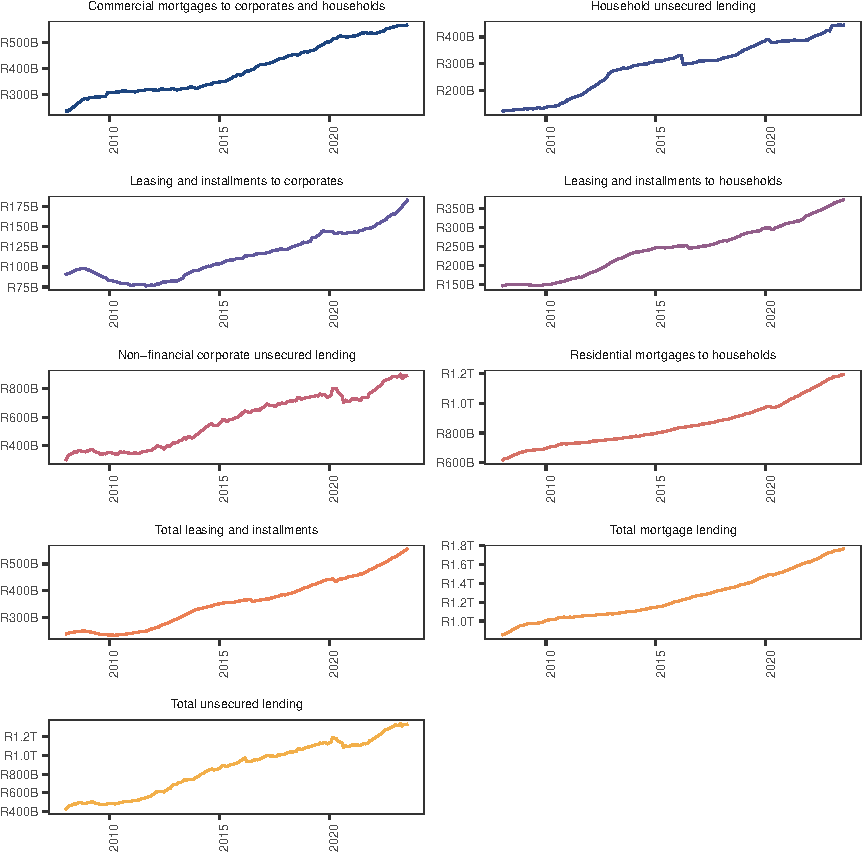
\includegraphics{UP_paper_v2_files/figure-pdf/fig-bank_lending-1.pdf}

}

\caption{\label{fig-bank_lending}Total aggregated bank lending}

\end{figure}%

\subsection{Weighted lending rates
(aggregated)}\label{weighted-lending-rates-aggregated}

\begin{figure}[H]

\centering{

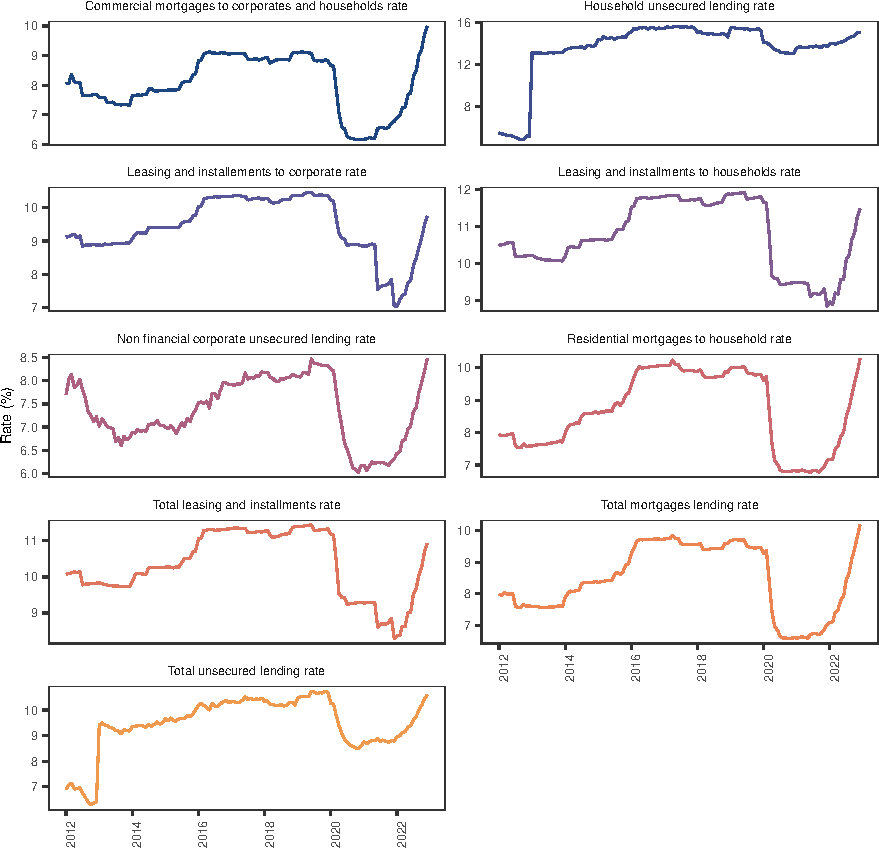
\includegraphics{UP_paper_v2_files/figure-pdf/fig-bank_interest_rates-1.pdf}

}

\caption{\label{fig-bank_interest_rates}Weighted lending rates}

\end{figure}%

\newpage

\subsection{Description of narrative
events}\label{description-of-narrative-events}

\subsubsection{Macroprudential
Indicators}\label{macroprudential-indicators}

This section provides a detailed account of the narrative
macroprudential indicators. The asterisk (*) indicates that the specific
regulation is tracked from the date of announcement to the date of
implementation.

2008/01/01: \textcolor{ForestGreen}{Implementation}

\begin{quote}
            BASEL II is  Implemented until Dec 2011
\end{quote}

2009/02/04:
\textcolor{blue}{Announcement, draft and passing of regulation}

\begin{quote}SARB issues  \textbf{directive 1/2009 (1 of 2009)} announcing the approach banks should follow in the application of capital floors. "Modelled capital should not be below 80\% of the capital requirements under Basel I to ensure capital levels do not fall below prudent level". Following Basel II, banks are allowed to use internal models to determine risk weights and in turn, determine capital levels. However, capital floors ensure capital requirements did not fall below a certain percentage of banks’ capital requirements under the previous Basel I framework\citep{basel06}. This in essence, imply greater risk weight attached to riskier credit products. For instance,  \cite{imbierowicz2018time} show that Danish banks reducing their lending on loans with higher risk weights, in response to higher capital requirements, including approaches to capital floors.
 \end{quote}

2009/07/31*:
\textcolor{blue}{Announcement, draft and passing of regulation}

\begin{quote}BCBS announces "measures to strengthen the 1996 rules governing trading book capital and to enhance the three pillars of the Basel II framework (Basel 2.5)". This in essence, aims  to introduce higher capital requirements to capture the credit risk of complex trading activities, promote the build-up of capital buffers that can be drawn down in periods of stress and strengthen the quality of bank capital\citep{basel09}
                \end{quote}

2010/10/08*:
\textcolor{blue}{Announcement, draft and passing of regulation}

\begin{quote}SARB issues \textbf{circular 3/2010} endorsing and giving notices to banks to prepare for the implementation of Basel 2.5, following the communication by the BCBS on July 31, 2009

\end{quote}

2011/06/30*:
\textcolor{blue}{Announcement, draft and passing of regulation}

\begin{quote}BCBS issues and publishes Basel III: A Global Regulatory Framework for More Resilient Banks and Banking Systems.
\end{quote}

2011/07/31:
\textcolor{blue}{Announcement, draft and passing of regulation}

\begin{quote}
Cabinet adopts proposal to shift to Twin Peaks Model of Financial Regulation in South Africa, following he GFC, with the aim of improving  institutional structure to support financial regulation. This is a signal to stricter oversight on the overall financial system
\end{quote}

2011/10/31:
\textcolor{blue}{Announcement, draft and passing of regulation}

\begin{quote}
    Basel 2.5 is transposed into domestic law (next step is implementation)
\end{quote}

2012/01/01: \textcolor{ForestGreen}{Implementation}

\begin{quote}
    Basel 2.5 takes effect: SARB minimum capital requirements
    \begin{itemize}
        \item Total CET1, 5.25\%, Total Tier1, 7\%, Minimum regulatory capital, 8\%, Total regulatory capital for D-SIB, 9.5\%
    \end{itemize}
\end{quote}

2012/02/16*:
\textcolor{blue}{Announcement, draft and passing of regulation}

\begin{quote}

SARB issues \textbf{guidance note 2/2012} announcing on new definition of total regulatory capital for Basel III such as:
\begin{itemize}
    \item Phasing out arrangements for non-common equity Tier 1 capital instruments that no longer qualify as regulatory capital under Basel III
 \item Transitional arrangements for Basel III implementation
\item Treatment of disclosed reserves under Basel III

\end{itemize}
\end{quote}

2012/05/31*:
\textcolor{blue}{Announcement, draft and passing of regulation}

\begin{quote}
SARB issues \textbf{guidance Note G5/2012} announcing that it will provide  liquidity facility to assist banks in meeting the liquidity Coverage Ratio (LCR) and cash reserves can be included as banks' high quality liquid assets for calculating LCR. This follows results from Quantitative Impact Studies (QIS) exercises by banks,  which revealed some banks would have shortfalls of around R140 billion in meeting the 100\% LCR  by 1 Jan 2019 due do to reliance eon short-term funding limited availability of HQLA

\begin{itemize}
    \item LCR requirements will be introduced on \textbf{1 Jan 2015} at 60\%, increasing by 10\% to reach 100\% on 1 Jan 2019
\item Level 1 assets (stocks, funds or bonds) shall comprise 60\% of total HQLA  while level 2 assets (less liquid) shall constitute no more than the remaining 40\%
\item SARB proposes that Leverage ratio be set at 4\% (LR of 4\% implies that banks' leverage does not exceed its capital by 40\%)
\end{itemize}

\end{quote}

2012/08/15*:
\textcolor{blue}{Announcement, draft and passing of regulation}

\begin{quote}
SARB transposes Basel III into law and publishes Counter-cyclical Capital Buffer (CCyB) rules, set to be implemented on 1 January 2016
\end{quote}

2013/01/31/*: \textcolor{ForestGreen}{Implementation}

\begin{quote}
    Basel III takes effect
\end{quote}

2013/08/20:
\textcolor{blue}{Announcement, draft and passing of regulation}

\begin{quote}
 SARB issues \textbf{Guidance Note 6/2013} announcing that banks' cash reserves may be included as part of their level 1 HQLA. Only equities listed on JSE's main exchange and included on Top 40 Index shall be considered as level2 HQLA (\textit{Potentially limit banks' ability to raise capital}).
\end{quote}

2014/01/31: \textcolor{ForestGreen}{Implementation}

\begin{quote}
SARB mimimum Capital Requirements increase to:\\
Total CET1, 5,5\%, Total Tier1, 7\%, Total regulatory capital, 8\%, Total regulatory capital for D-SIB, 10\%
\end{quote}

2014/12/31:
\textcolor{blue}{Announcement, draft and passing of regulation}

\begin{quote}
SARB issues \textbf{guidance note 8/2014} announcing  the provision of a committed liquidity facility  (CLF). This is to assist banks to meet the LCR.
Banks, however need to have collateral to access the CLF, consisting of:
\begin{itemize}
    \item  High-quality residential mortgage loans
\item Other loans and advances such as VAF, excluding unsecured loans
\item Domestically listed securities
\end{itemize}
\end{quote}

2015/01/31*: \textcolor{ForestGreen}{Implementation}

\begin{quote}
LCR ratio is introduced/implemented at 60\% compliance
\end{quote}

2015/12/31*:
\textcolor{blue}{Announcement, draft and passing of regulation}

\begin{quote}
SARB issues \textbf{circular 8/2015} announcing timelines and targets in respect of  the implementation of the countercyclical capital buffer (CCyB). SARB requirements shall apply to bank-wide total RWA:
\begin{itemize}
    \item 0.625\% on 1 Jan 2016
\item 1.25\% 1 Jan 2017
\item 1.875\% on 1 Jan 2018
\item 2.5\% on 1 Jan 2019
\end{itemize}
\end{quote}

2016/01/31*: \textcolor{ForestGreen}{Implementation}

\begin{quote}
CCyB is implemented and set at 0.625\%
\end{quote}

2016/04/13*:
\textcolor{blue}{Announcement, draft and passing of regulation}

\begin{quote}
SARB issues \textbf{directive 1/2016} to inform all banks of matters related to the exposure limits imposed in the classification of deposits and credit exposures to small and medium enterprises  (SMEs), to be implemented on 1 July 2016. For instance, total exposure of a bank to an SME borrower, which shall be determined or calculated on a consolidated basis, at no time exceeds R12,5 million (\textit{Greater limits on value of a loan that can be extended to an SME})
\end{quote}

2016/07/01*: \textcolor{ForestGreen}{Implementation}

\begin{quote}
Exposure limits imposed in the classification of deposits and credit exposures to small and medium enterprises  (SMEs), announced on 2016/04/13, is implemented
\end{quote}

2017/01/31*: \textcolor{ForestGreen}{Implementation}

\begin{quote}
LCR ratio is introduced/implemented at 80\% compliance, while CCyB increases to 1.25\%
\end{quote}

\begin{quote}
2017/12/13*: \textcolor{blue}{Announcement, draft and passing of regulation}
SARB issues \textbf{directive 8/2017} informing banks to comply with the Net Stable Funding Ratio (NSFR) framework and on matters related to calibration of NSFR, including  template to monitor NSFR compliance. Agrees to start implementation on 1 January 2018. Objective is to reduce funding risk over a longer time horizon by requiring banks to fund their activities with sufficiently stable sources of funding in order to mitigate the risk of future funding stress. \textit{Banks will be required to match their funding with their outflows, which may lead to a greater demand for longer term funding. Longer term funding will result in an increased cost of funding for banks (possibly passed on to borrowers and lower profitability and returns for banks}
\end{quote}

2018/01/31*: \textcolor{ForestGreen}{Implementation}

\begin{quote}
NSFR Implemented following  Directive 8/2017, CCyB increases to 1,875\% and LCR is implemented at 90\% compliance.
\end{quote}

2019/01/31*: \textcolor{ForestGreen}{Implementation}

\begin{quote}
CCyB increases to 2,5\% (maximum) and LCR is implemented at 100\% compliance.
\end{quote}

\newpage

\subsubsection{Finance regulation index}\label{finance-regulation-index}

\textbf{Changes in the National Credit Act of 2005 Regulations}

The National Credit Act of 2005 is legislation that was enacted in order
to better regulate the markets for customer credit. According to this
Act its purpose is to develop, inter alia, credit markets that are
accessible by all South Africans, correct the imbalance in negotiating
power between consumers and credit providers, regulate the collection
and sharing of consumer credit information and prevent
over-indebtedness. These, and other, efforts are to achieve a
\emph{``fair, transparent, competitive, sustainable, responsible,
efficient, effective and accessible credit market and industry, and to
protect consumers}\footnote{Section 3 of the NCA.}. The Act specifically
provided the Minister of, the erstwhile, Trade and Industry with powers
to provide regulations pertaining to the implementation of the
Act.\footnote{Section 171 of the NCA.} These regulations were made
available in May 2006.

The initial regulations pre-date the period assessed by this paper, but
the proposed and later realised changes to these Regulations occurred
between 2012 and 2015. It is these developments that are captured within
\(FinReg\).

\emph{2012 Debt Counselling Regulations}

On the 10th of May 2012 the Minister of Trade and Industry published
debt counselling regulations. These codified the process to be followed
by debt counselors and consumers when seeking various order from the
Magistrate's Court. These orders relate to the re-structuring of debt
following a debt counselor's findings of consumer over-indebtedness,
consumer difficulty to meet debt obligations and direct applications by
consumers to the court following an adverse finding by debt counsellors.
The regulations also provided that credit providers were expected to
implement orders from the Court within 10 working days following their
receipt of the court orders from the debt counselors and/or consumers
\citep{regulations2012}.\footnote{The initial draft regulations were
  published on the 15th of May 2009 and did not prescribe the period
  within which court orders, made following debt counselling processes,
  were to be implemented by credit providers}.

\citet{roestoff2009} indicates that provisions of the National Credit
Act in regard to debt relief are to assist over-indebted consumers,
prioritising their interests more than those of credit providers. To
achieve these outcomes, debt review negotiations require that credit
providers have greater responsibility toward the possible negative
outcomes of credit provision.

\emph{2013 and 2014 draft and final credit regulations on the removal of
adverse consumer credit information and information relating to paid up
judgements}

In 2013 the Minister of Trade and Industry issued a notice about a
proposal to remove adverse credit information from credit bureaus. This
followed Cabinet endorsement of a \emph{Removal of Adverse Credit
Information Project}. The Minister proposed that all adverse findings
were to be removed regardless of non-payment. Thereafter on an ongoing
basis adverse information held by credit bureaus were on settled debt or
paid up judgements were to be removed. Communication from the SA
government indicated that this move was to ensure that those who could
access credit, and were prevented from doing so, due to adverse credit
information could do so \citep{sagov2013}.

On the 26th of February 2014, the Minister published final regulations
instructing credit bureaus that adverse credit information was to be
removed on all paid up judgements \citep{regulations2014a}. The final
regulations were less ambitious than the proposal. Nevertheless, the
\citet{ncrnd} indicates that the regulations were to enable consumer
access to affordable credit, as well as employment opportunities.

\emph{2014 and 2015 changes to the National Credit Regulations}

On the 1st of August 2014, the Minister of Trade and Industry published
draft national credit regulations that proposed a host of changes to the
existing 2006 regulations, as amended \citep{regulations2014b}. Many of
these were proposed insertions into the regulations that did not exist
before. The proposals included a criteria to be adopted by credit
providers to conduct affordability assessments to further limit
instances of reckless lending. Credit providers were provided with
additional limits on when adverse consumer credit information was to be
shared with credit bureaus; for instance, information that consumers did
not meet their financial obligations would not be shared unless a
consumer would have missed their minimum obligations for three
consecutive months. Related to credit bureau information were changes to
the maximum periods that credit information were to be kept by credit
bureaus. For many of the types of information kept, the proposed
regulations proposed reduced retention periods. For instance,
information relating to enquiries on a consumers record was to be
reduced from 2 years to 2 months; information on liquidations had been
kept for an unlimited period and the proposal was to reduce this to 5
years; information on complaints initiated by customers was kept from 18
months and proposed to be reduced to 6 months. Other changes included
explicit references to the registration and operation of payment
distribution agents, as well as the provision of clarity on when credit
information could be obtained for employment purposes.

By the 13th of March 2015, the Minister provided a final set of proposed
changes and insertions into the regulations that would come into effect
\citep{regulations2015a}. Many of the 2014 proposals were accepted, some
with changes. Some of these included the explicit criteria for
affordability assessments, changes to the retention periods for credit
bureau information, and the additional limits on when adverse consumer
credit information was to be shared with credit bureaus.

\emph{2015 draft and final credit regulations on limitations on fees and
interest rates}

Section 42(1) of the 2006 credit regulations provided the maximum
interest rates to be set on different types of credit
\citep{regulations2006}. These included mortgages, credit facilities,
unsecured credit, developmental credit, short term credit, other and
incidental credit agreements. Incidental and short term credit rates
were respectively capped at 2\% and 5\% per month. The limits for other
rates were calculated at the repo rate scaled up by 2.2 and increased by
fixed interest rates ranging between 5 to 20 percentage points depending
on the credit type. In addition, the regulations also provided the
maximum Rand values that would be set as initiation and service fees.
The initiation fees varied by credit type.

In 2015, the Minister of Trade and Industry proposed changes to these
interest rates and initiation fees \citep{regulations2015b}. Final
changes came into effects that same year \citep{regulations2015c}. For 5
of the 7 credit types, the Minister provided a lower scalar by higher
interest rate premium. The net effect of this adjustment was that
maximum interest rates on credit facilities would be lower by 2.9
percentage points and 7.9 percentage points for unsecured credit (based
on the prevailing repo rate). The maximum rates set for other credit
types increased marginally by 0.1 percentage points of had no change at
all. Initiation and service fees were increased above the limits set in
the 2006 regulations.

\textbf{Restructuring of the financial sector regulation}

\emph{Financial Sector Regulation Act}

The Financial Sector Regulation Act of 2017 represented a structural
shift in the regulation of financial institutions in South Africa, as it
set up a framework for financial regulation and supervision.

The Act importantly sets up two authorities with important regulatory
powers. One is the Prudential Authority, which sits within the South
African Reserve Bank. This object of this authority is to ensure the
soundness of financial institutions and infrastructure and financial
stability, as well as protecting consumers against risks from financial
institutions. The other authority created by the act is the Financial
Sector Conduct Authority (FSCA).\footnote{The FSCA replaced the
  Financial Services Board. See:
  https://www.fsca.co.za/TPNL/4/fsb4/proactive.html} The object of the
FSCA was to protect financial consumers by promoting fair treatment and
financial education, as well as to maintaining financial stability and
market efficiency.

Both the PA and the FSCA were tasked with promoting financial inclusion.
Which the Act defined as a state where all persons have access to
\emph{``timely and fair access to appropriate, fair and affordable
financial products and services''} \citep{fsr2017}.

\emph{Draft and Update of the Conduct of Financial Institutions Bill}

In 2018 the National Treasury presented a draft Conduct of Financial
Institutions (COFI) Bill. This bill proposes consolidating a number of
the financial sector laws of the country. At present, the nature of
financial sector regulation is focused on particular sectors. For
instance, insurance companies are regulated by the Insurance Act,
investment schemes by the Collective Investment Schemes Control Act and
financial service providers by the Financial Advisory and Intermediary
Services Act. The proposed bill seeks to provide the provide the
Financial Services Conduct Authority with the ability to regulate the
conduct of institution that provide the similar services and products
\citep{cofi2018a}.

With regard to credit provision, the COFI bill proposes providing the
FSCA with the ability to provide standards for the conduct of firms in
the provision of financial products and services. The referred to
conduct relates to, inter alia, firms' charging structures, pricing
methodologies, financial product features and the identification of
appropriate and inappropriate target markets
\citep[\citet{cofi2020}]{cofi2018a}. The \citet{cofi2018b} explains that
this proposed legislation is premised on supporting greater financial
inclusion as the better regulation of firm conduct would provide
consumers with greater security required for their usage of financial
sector products. A draft COFI bill was presented in 2018 and an updated
draft in 2020 \citep{cofi2020}.

\textbf{National financial inclusion policy}

\emph{Draft Financial Inclusion Policy Report is published}

In 2020 the National Treasury provided a draft national policy framework
for financial inclusion in South Africa. The existing state of financial
inclusion is reported to be high in South Africa but the National
Treasury notes that the usage of financial products by low income
earners remains low and that small, medium and micro enterprises are
only marginally serviced \citep{nt2020}. On the back of these
challenges, the draft national policy framework provides the initiatives
to be support the three key pillars they identify as being important to
financial inclusion: (i) deepening financial inclusion, (ii) improving
access for SMMEs and (iii) supporting more diverse providers of
financial services.

A number of initiatives identified by the \citet{nt2020} in the above
mentioned three pillars relate directly to credit currently extended by
incumbent banks. To increase developmental loans provided to low income
families, the policy proposes governments sharing losses on defaults and
a students future income to assess affordability of loans, as well as
the use of different forms of collateral (such as a permission to
occupy) to secure mortgage financing. SMME access to financing is
planned to be supported by improvements in credit infrastructure for
small businesses; an example of this will include consideration of SMME
payments data as information relevant to determining ability to access
credit. To support more providers of financial services \citet{nt2020}
proposes promoting the development of cooperative banks to compete
against incumbent banks, developing a licensing framework that supports
the entry of new financial institutions and assessing the role of a
state owned bank.

The financial inclusion policy sets out a number of initiatives that are
likely to have an impact when and how incumbent banks extend credit. In
addition, the proposed framework as suggests various programmes that
would create additional financial institutions that are likely to
compete with incumbents in markets relating to credit provision.

\subsection{Macroprudential narrative
indexes}\label{macroprudential-narrative-indexes}

\begin{figure}[H]

\centering{

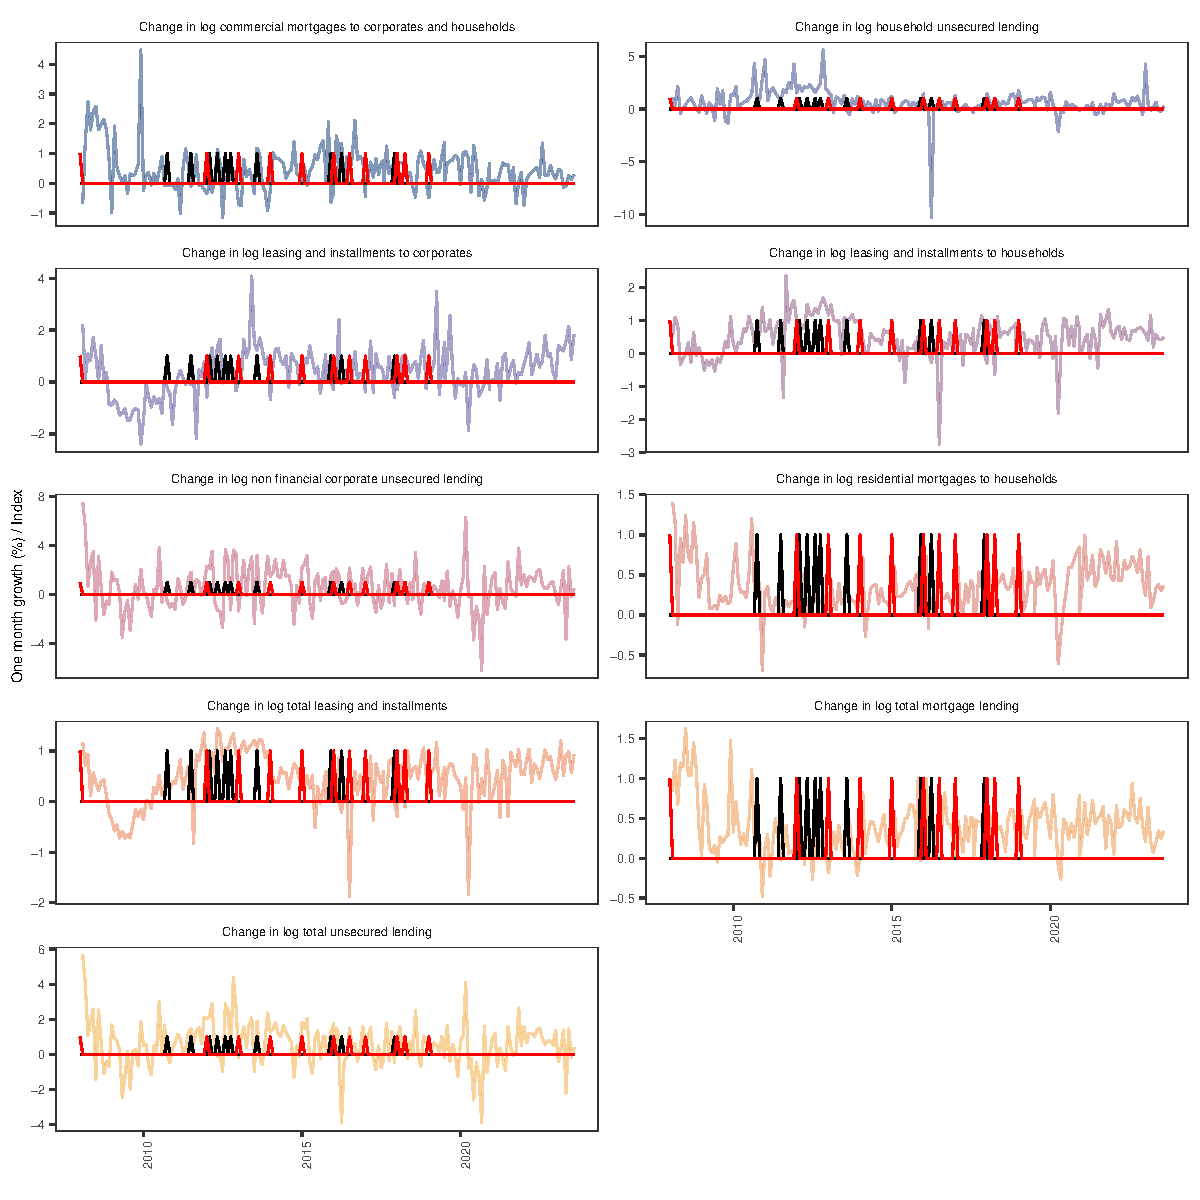
\includegraphics{UP_paper_v2_files/figure-pdf/fig-macro_narrative_indexes_one_month-1.pdf}

}

\caption{\label{fig-macro_narrative_indexes_one_month}One month lending
growth and macroprudential narrative index comparison. Note: The black
line represents the Draft index, and the red line represents the
Implementation index.}

\end{figure}%

\newpage

\begin{figure}[H]

\centering{

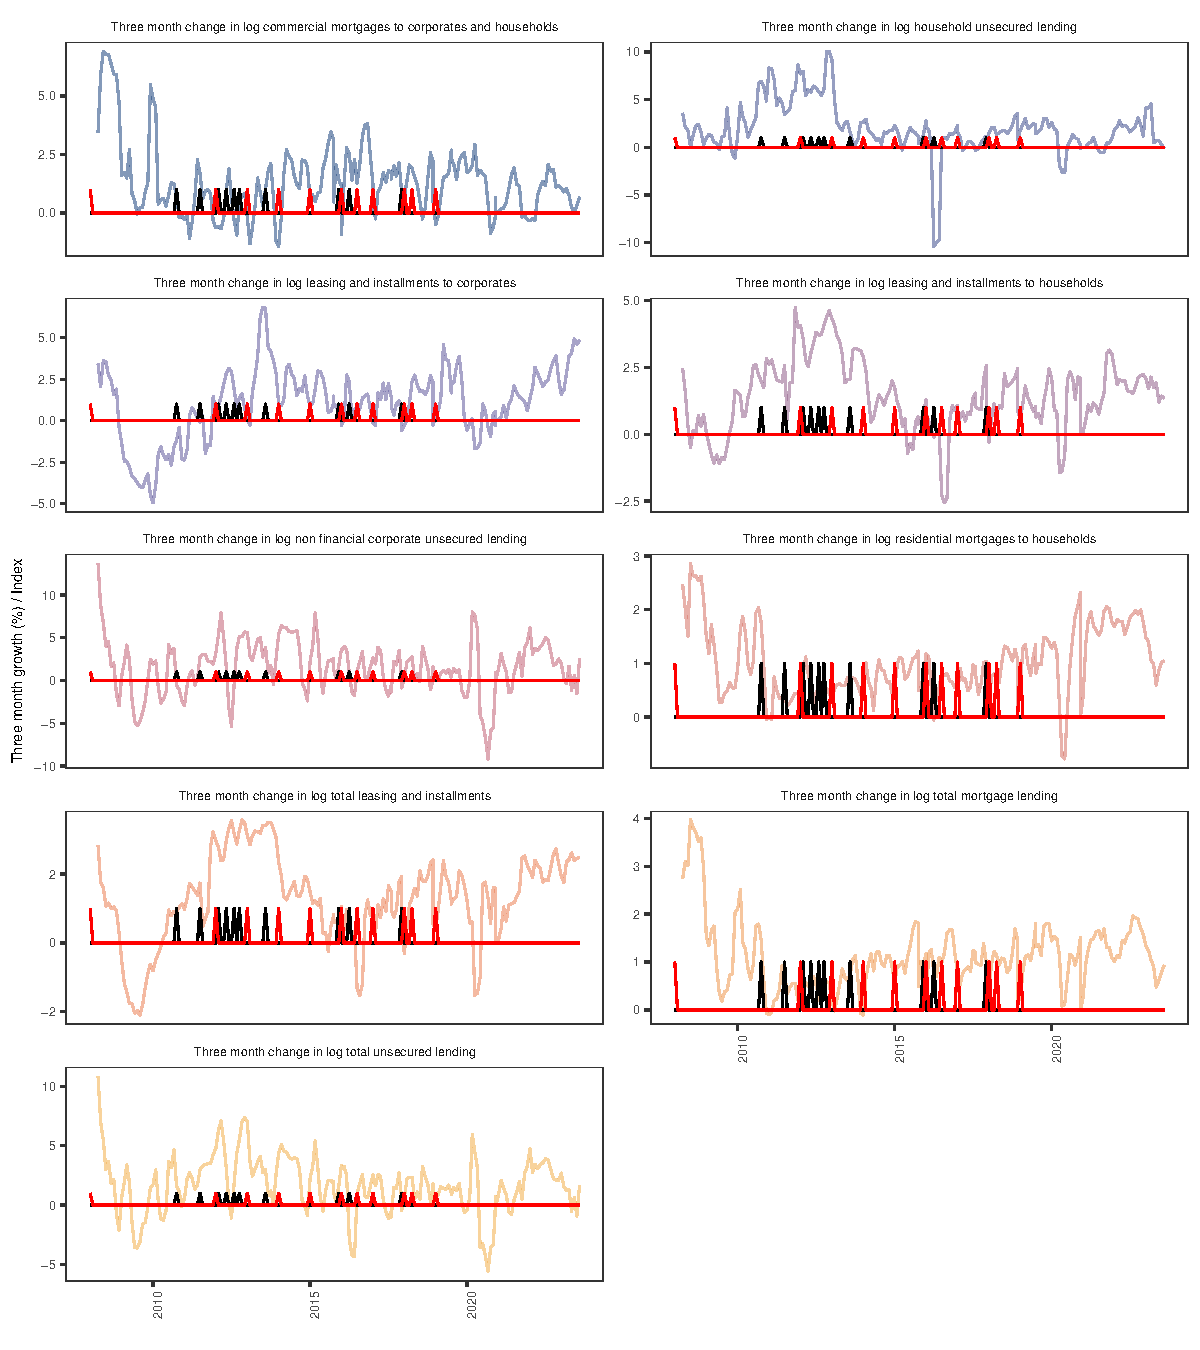
\includegraphics{UP_paper_v2_files/figure-pdf/fig-macro_narrative_indexes_three_month-1.pdf}

}

\caption{\label{fig-macro_narrative_indexes_three_month}Three month
lending growth and macroprudential narrative indexes comparison. Note:
The black line represents the Draft index, and the red line represents
the Implementation index.}

\end{figure}%

\newpage

\subsection{Financial regulation narrative
indexes}\label{financial-regulation-narrative-indexes}

\begin{figure}[H]

\centering{

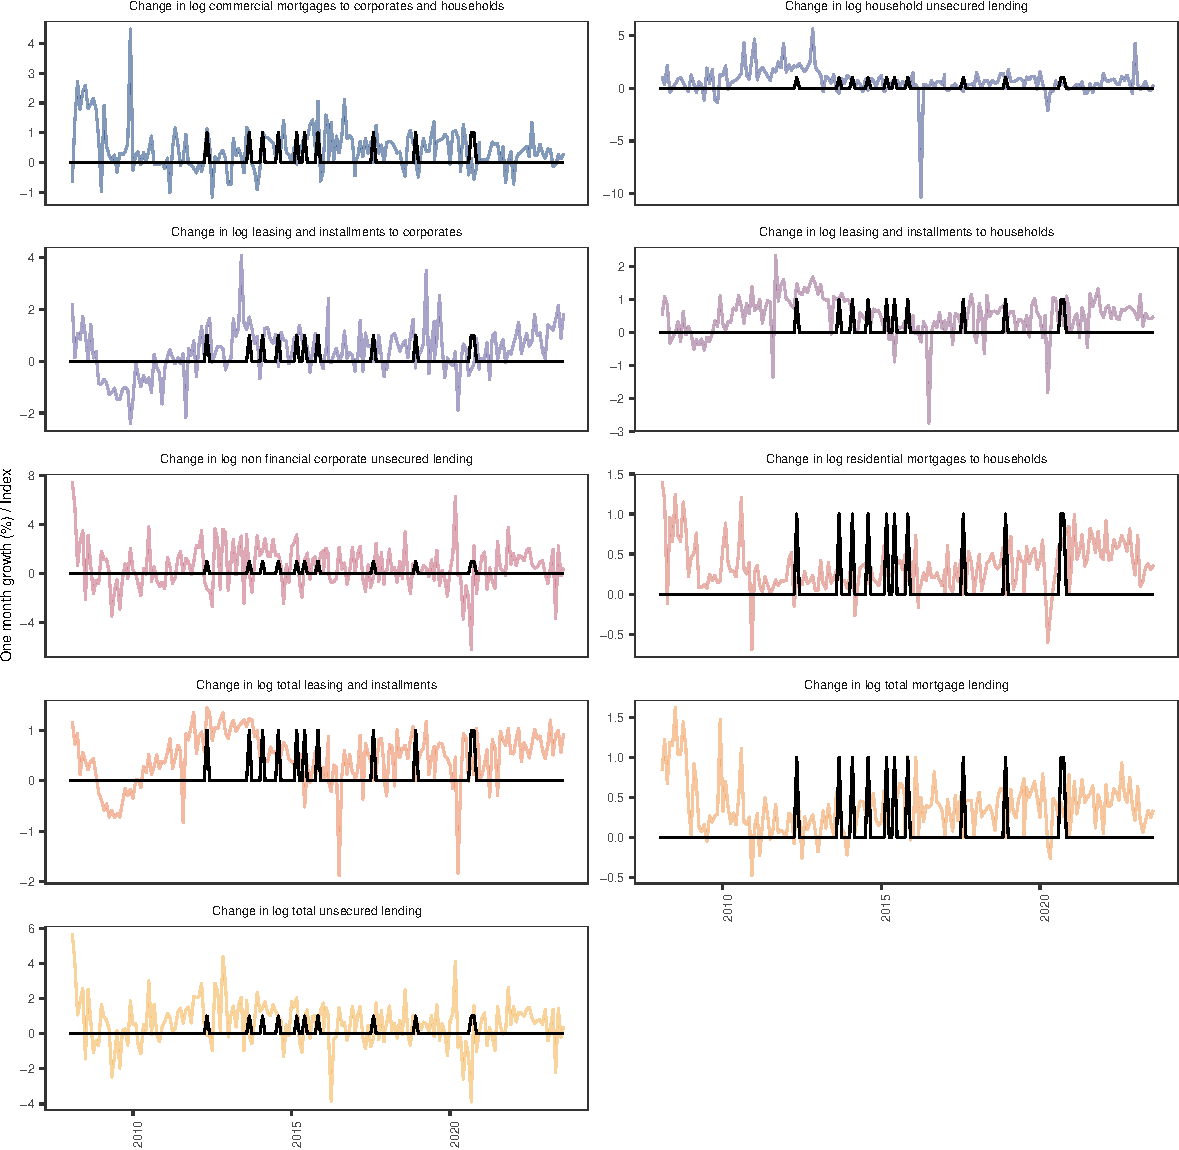
\includegraphics{UP_paper_v2_files/figure-pdf/fig-comp_narrative_indexes_one_month-1.pdf}

}

\caption{\label{fig-comp_narrative_indexes_one_month}One month lending
growth and financial narrative index comparison. Note: The black line
represents the Financial regulation index.}

\end{figure}%

\newpage

\begin{figure}[H]

\centering{

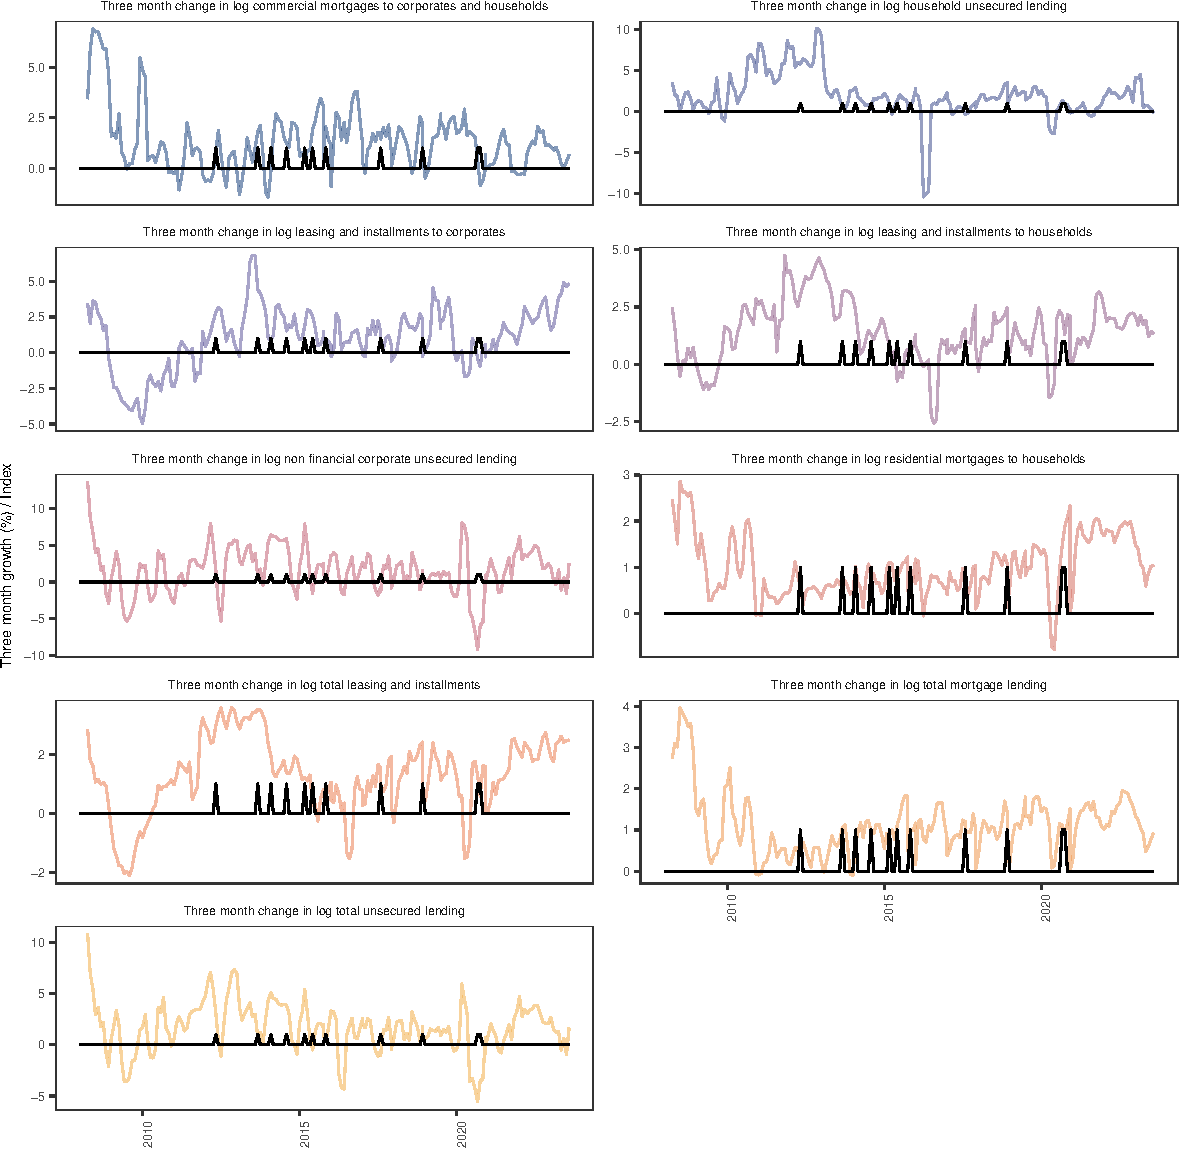
\includegraphics{UP_paper_v2_files/figure-pdf/fig-comp_narrative_indexes_three_month-1.pdf}

}

\caption{\label{fig-comp_narrative_indexes_three_month}Three month
lending growth and financial narrative indexes comparison. Note: The
black line represents the Financial regulation index.}

\end{figure}%

\newpage

\bsideways

\subsection{Results with controls}\label{results-with-controls}

\global\setlength{\Oldarrayrulewidth}{\arrayrulewidth}

\global\setlength{\Oldtabcolsep}{\tabcolsep}

\setlength{\tabcolsep}{2pt}

\renewcommand*{\arraystretch}{1}



\providecommand{\ascline}[3]{\noalign{\global\arrayrulewidth #1}\arrayrulecolor[HTML]{#2}\cline{#3}}

\begin{longtable}[l]{|p{1.40in}|p{0.75in}|p{0.75in}|p{0.75in}|p{0.75in}|p{0.75in}|p{0.75in}|p{0.75in}|p{0.75in}|p{0.75in}}

\caption{\label{tbl-macropru_draft_rates_control}Macroprudential
regulation and lending rates with controls results}

\tabularnewline

\ascline{1pt}{000000}{1-10}

\multicolumn{1}{>{\centering}m{\dimexpr 1.4in+0\tabcolsep}}{\textcolor[HTML]{000000}{\fontsize{7}{7}\selectfont{\global\setmainfont{Arial}{}}}} & \multicolumn{3}{!{\color[HTML]{FFFFFF}\vrule width 1pt}>{\centering}m{\dimexpr 2.25in+4\tabcolsep+2pt}}{\textcolor[HTML]{000000}{\fontsize{7}{7}\selectfont{\global\setmainfont{Arial}{Total}}}} & \multicolumn{3}{!{\color[HTML]{FFFFFF}\vrule width 1pt}>{\centering}m{\dimexpr 2.25in+4\tabcolsep+2pt}}{\textcolor[HTML]{000000}{\fontsize{7}{7}\selectfont{\global\setmainfont{Arial}{Corporations}}}} & \multicolumn{3}{!{\color[HTML]{FFFFFF}\vrule width 1pt}>{\centering}m{\dimexpr 2.25in+4\tabcolsep+2pt}!{\color[HTML]{FFFFFF}\vrule width 1pt}}{\textcolor[HTML]{000000}{\fontsize{7}{7}\selectfont{\global\setmainfont{Arial}{Households}}}} \\

\ascline{1pt}{FFFFFF}{1-1}\ascline{1pt}{000000}{2-10}



\multicolumn{1}{>{\raggedright}m{\dimexpr 1.4in+0\tabcolsep}}{\textcolor[HTML]{000000}{\fontsize{7}{7}\selectfont{\global\setmainfont{Arial}{\ }}}} & \multicolumn{1}{!{\color[HTML]{FFFFFF}\vrule width 1pt}>{\raggedright}m{\dimexpr 0.75in+0\tabcolsep}}{\textcolor[HTML]{000000}{\fontsize{7}{7}\selectfont{\global\setmainfont{Arial}{Unsecured}}}} & \multicolumn{1}{!{\color[HTML]{FFFFFF}\vrule width 1pt}>{\raggedright}m{\dimexpr 0.75in+0\tabcolsep}}{\textcolor[HTML]{000000}{\fontsize{7}{7}\selectfont{\global\setmainfont{Arial}{Secured}}}} & \multicolumn{1}{!{\color[HTML]{FFFFFF}\vrule width 1pt}>{\raggedright}m{\dimexpr 0.75in+0\tabcolsep}}{\textcolor[HTML]{000000}{\fontsize{7}{7}\selectfont{\global\setmainfont{Arial}{Mortgage}}}} & \multicolumn{1}{!{\color[HTML]{FFFFFF}\vrule width 1pt}>{\raggedright}m{\dimexpr 0.75in+0\tabcolsep}}{\textcolor[HTML]{000000}{\fontsize{7}{7}\selectfont{\global\setmainfont{Arial}{Unsecured}}}} & \multicolumn{1}{!{\color[HTML]{FFFFFF}\vrule width 1pt}>{\raggedright}m{\dimexpr 0.75in+0\tabcolsep}}{\textcolor[HTML]{000000}{\fontsize{7}{7}\selectfont{\global\setmainfont{Arial}{Secured}}}} & \multicolumn{1}{!{\color[HTML]{FFFFFF}\vrule width 1pt}>{\raggedright}m{\dimexpr 0.75in+0\tabcolsep}}{\textcolor[HTML]{000000}{\fontsize{7}{7}\selectfont{\global\setmainfont{Arial}{Mortgage}}}} & \multicolumn{1}{!{\color[HTML]{FFFFFF}\vrule width 1pt}>{\raggedright}m{\dimexpr 0.75in+0\tabcolsep}}{\textcolor[HTML]{000000}{\fontsize{7}{7}\selectfont{\global\setmainfont{Arial}{Unsecured}}}} & \multicolumn{1}{!{\color[HTML]{FFFFFF}\vrule width 1pt}>{\raggedright}m{\dimexpr 0.75in+0\tabcolsep}}{\textcolor[HTML]{000000}{\fontsize{7}{7}\selectfont{\global\setmainfont{Arial}{Secured}}}} & \multicolumn{1}{!{\color[HTML]{FFFFFF}\vrule width 1pt}>{\raggedright}m{\dimexpr 0.75in+0\tabcolsep}}{\textcolor[HTML]{000000}{\fontsize{7}{7}\selectfont{\global\setmainfont{Arial}{Mortgage}}}} \\

\ascline{1pt}{000000}{1-10}\endfirsthead 

\ascline{1pt}{000000}{1-10}

\multicolumn{1}{>{\centering}m{\dimexpr 1.4in+0\tabcolsep}}{\textcolor[HTML]{000000}{\fontsize{7}{7}\selectfont{\global\setmainfont{Arial}{}}}} & \multicolumn{3}{!{\color[HTML]{FFFFFF}\vrule width 1pt}>{\centering}m{\dimexpr 2.25in+4\tabcolsep+2pt}}{\textcolor[HTML]{000000}{\fontsize{7}{7}\selectfont{\global\setmainfont{Arial}{Total}}}} & \multicolumn{3}{!{\color[HTML]{FFFFFF}\vrule width 1pt}>{\centering}m{\dimexpr 2.25in+4\tabcolsep+2pt}}{\textcolor[HTML]{000000}{\fontsize{7}{7}\selectfont{\global\setmainfont{Arial}{Corporations}}}} & \multicolumn{3}{!{\color[HTML]{FFFFFF}\vrule width 1pt}>{\centering}m{\dimexpr 2.25in+4\tabcolsep+2pt}!{\color[HTML]{FFFFFF}\vrule width 1pt}}{\textcolor[HTML]{000000}{\fontsize{7}{7}\selectfont{\global\setmainfont{Arial}{Households}}}} \\

\ascline{1pt}{FFFFFF}{1-1}\ascline{1pt}{000000}{2-10}



\multicolumn{1}{>{\raggedright}m{\dimexpr 1.4in+0\tabcolsep}}{\textcolor[HTML]{000000}{\fontsize{7}{7}\selectfont{\global\setmainfont{Arial}{\ }}}} & \multicolumn{1}{!{\color[HTML]{FFFFFF}\vrule width 1pt}>{\raggedright}m{\dimexpr 0.75in+0\tabcolsep}}{\textcolor[HTML]{000000}{\fontsize{7}{7}\selectfont{\global\setmainfont{Arial}{Unsecured}}}} & \multicolumn{1}{!{\color[HTML]{FFFFFF}\vrule width 1pt}>{\raggedright}m{\dimexpr 0.75in+0\tabcolsep}}{\textcolor[HTML]{000000}{\fontsize{7}{7}\selectfont{\global\setmainfont{Arial}{Secured}}}} & \multicolumn{1}{!{\color[HTML]{FFFFFF}\vrule width 1pt}>{\raggedright}m{\dimexpr 0.75in+0\tabcolsep}}{\textcolor[HTML]{000000}{\fontsize{7}{7}\selectfont{\global\setmainfont{Arial}{Mortgage}}}} & \multicolumn{1}{!{\color[HTML]{FFFFFF}\vrule width 1pt}>{\raggedright}m{\dimexpr 0.75in+0\tabcolsep}}{\textcolor[HTML]{000000}{\fontsize{7}{7}\selectfont{\global\setmainfont{Arial}{Unsecured}}}} & \multicolumn{1}{!{\color[HTML]{FFFFFF}\vrule width 1pt}>{\raggedright}m{\dimexpr 0.75in+0\tabcolsep}}{\textcolor[HTML]{000000}{\fontsize{7}{7}\selectfont{\global\setmainfont{Arial}{Secured}}}} & \multicolumn{1}{!{\color[HTML]{FFFFFF}\vrule width 1pt}>{\raggedright}m{\dimexpr 0.75in+0\tabcolsep}}{\textcolor[HTML]{000000}{\fontsize{7}{7}\selectfont{\global\setmainfont{Arial}{Mortgage}}}} & \multicolumn{1}{!{\color[HTML]{FFFFFF}\vrule width 1pt}>{\raggedright}m{\dimexpr 0.75in+0\tabcolsep}}{\textcolor[HTML]{000000}{\fontsize{7}{7}\selectfont{\global\setmainfont{Arial}{Unsecured}}}} & \multicolumn{1}{!{\color[HTML]{FFFFFF}\vrule width 1pt}>{\raggedright}m{\dimexpr 0.75in+0\tabcolsep}}{\textcolor[HTML]{000000}{\fontsize{7}{7}\selectfont{\global\setmainfont{Arial}{Secured}}}} & \multicolumn{1}{!{\color[HTML]{FFFFFF}\vrule width 1pt}>{\raggedright}m{\dimexpr 0.75in+0\tabcolsep}}{\textcolor[HTML]{000000}{\fontsize{7}{7}\selectfont{\global\setmainfont{Arial}{Mortgage}}}} \\

\ascline{1pt}{000000}{1-10}\endhead



\multicolumn{10}{>{\centering}m{\dimexpr 8.15in+18\tabcolsep+9pt}!{\color[HTML]{FFFFFF}\vrule width 1pt}}{\textcolor[HTML]{000000}{\fontsize{7}{7}\selectfont{\global\setmainfont{Arial}{Draft\ model}}}} \\

\ascline{1pt}{FFFFFF}{1-10}



\multicolumn{1}{>{\raggedright}m{\dimexpr 1.4in+0\tabcolsep}}{\textcolor[HTML]{000000}{\fontsize{7}{7}\selectfont{\global\setmainfont{Arial}{Draft\ index}}}} & \multicolumn{1}{!{\color[HTML]{FFFFFF}\vrule width 1pt}>{\raggedright}m{\dimexpr 0.75in+0\tabcolsep}}{\textcolor[HTML]{000000}{\fontsize{7}{7}\selectfont{\global\setmainfont{Arial}{0.420*}}}} & \multicolumn{1}{!{\color[HTML]{FFFFFF}\vrule width 1pt}>{\raggedright}m{\dimexpr 0.75in+0\tabcolsep}}{\textcolor[HTML]{000000}{\fontsize{7}{7}\selectfont{\global\setmainfont{Arial}{-0.378***}}}} & \multicolumn{1}{!{\color[HTML]{FFFFFF}\vrule width 1pt}>{\raggedright}m{\dimexpr 0.75in+0\tabcolsep}}{\textcolor[HTML]{000000}{\fontsize{7}{7}\selectfont{\global\setmainfont{Arial}{-0.472***}}}} & \multicolumn{1}{!{\color[HTML]{FFFFFF}\vrule width 1pt}>{\raggedright}m{\dimexpr 0.75in+0\tabcolsep}}{\textcolor[HTML]{000000}{\fontsize{7}{7}\selectfont{\global\setmainfont{Arial}{0.378}}}} & \multicolumn{1}{!{\color[HTML]{FFFFFF}\vrule width 1pt}>{\raggedright}m{\dimexpr 0.75in+0\tabcolsep}}{\textcolor[HTML]{000000}{\fontsize{7}{7}\selectfont{\global\setmainfont{Arial}{-0.441***}}}} & \multicolumn{1}{!{\color[HTML]{FFFFFF}\vrule width 1pt}>{\raggedright}m{\dimexpr 0.75in+0\tabcolsep}}{\textcolor[HTML]{000000}{\fontsize{7}{7}\selectfont{\global\setmainfont{Arial}{-0.182}}}} & \multicolumn{1}{!{\color[HTML]{FFFFFF}\vrule width 1pt}>{\raggedright}m{\dimexpr 0.75in+0\tabcolsep}}{\textcolor[HTML]{000000}{\fontsize{7}{7}\selectfont{\global\setmainfont{Arial}{0.404**}}}} & \multicolumn{1}{!{\color[HTML]{FFFFFF}\vrule width 1pt}>{\raggedright}m{\dimexpr 0.75in+0\tabcolsep}}{\textcolor[HTML]{000000}{\fontsize{7}{7}\selectfont{\global\setmainfont{Arial}{-0.350***}}}} & \multicolumn{1}{!{\color[HTML]{FFFFFF}\vrule width 1pt}>{\raggedright}m{\dimexpr 0.75in+0\tabcolsep}}{\textcolor[HTML]{000000}{\fontsize{7}{7}\selectfont{\global\setmainfont{Arial}{-0.571***}}}} \\

\ascline{1pt}{FFFFFF}{1-10}



\multicolumn{1}{>{\raggedright}m{\dimexpr 1.4in+0\tabcolsep}}{\textcolor[HTML]{000000}{\fontsize{7}{7}\selectfont{\global\setmainfont{Arial}{Return\ on\ assets}}}} & \multicolumn{1}{!{\color[HTML]{FFFFFF}\vrule width 1pt}>{\raggedright}m{\dimexpr 0.75in+0\tabcolsep}}{\textcolor[HTML]{000000}{\fontsize{7}{7}\selectfont{\global\setmainfont{Arial}{5.847***}}}} & \multicolumn{1}{!{\color[HTML]{FFFFFF}\vrule width 1pt}>{\raggedright}m{\dimexpr 0.75in+0\tabcolsep}}{\textcolor[HTML]{000000}{\fontsize{7}{7}\selectfont{\global\setmainfont{Arial}{-0.791**}}}} & \multicolumn{1}{!{\color[HTML]{FFFFFF}\vrule width 1pt}>{\raggedright}m{\dimexpr 0.75in+0\tabcolsep}}{\textcolor[HTML]{000000}{\fontsize{7}{7}\selectfont{\global\setmainfont{Arial}{-1.211}}}} & \multicolumn{1}{!{\color[HTML]{FFFFFF}\vrule width 1pt}>{\raggedright}m{\dimexpr 0.75in+0\tabcolsep}}{\textcolor[HTML]{000000}{\fontsize{7}{7}\selectfont{\global\setmainfont{Arial}{5.155***}}}} & \multicolumn{1}{!{\color[HTML]{FFFFFF}\vrule width 1pt}>{\raggedright}m{\dimexpr 0.75in+0\tabcolsep}}{\textcolor[HTML]{000000}{\fontsize{7}{7}\selectfont{\global\setmainfont{Arial}{-1.073}}}} & \multicolumn{1}{!{\color[HTML]{FFFFFF}\vrule width 1pt}>{\raggedright}m{\dimexpr 0.75in+0\tabcolsep}}{\textcolor[HTML]{000000}{\fontsize{7}{7}\selectfont{\global\setmainfont{Arial}{-1.124}}}} & \multicolumn{1}{!{\color[HTML]{FFFFFF}\vrule width 1pt}>{\raggedright}m{\dimexpr 0.75in+0\tabcolsep}}{\textcolor[HTML]{000000}{\fontsize{7}{7}\selectfont{\global\setmainfont{Arial}{6.013***}}}} & \multicolumn{1}{!{\color[HTML]{FFFFFF}\vrule width 1pt}>{\raggedright}m{\dimexpr 0.75in+0\tabcolsep}}{\textcolor[HTML]{000000}{\fontsize{7}{7}\selectfont{\global\setmainfont{Arial}{-0.643***}}}} & \multicolumn{1}{!{\color[HTML]{FFFFFF}\vrule width 1pt}>{\raggedright}m{\dimexpr 0.75in+0\tabcolsep}}{\textcolor[HTML]{000000}{\fontsize{7}{7}\selectfont{\global\setmainfont{Arial}{-1.285}}}} \\

\ascline{1pt}{FFFFFF}{1-10}



\multicolumn{1}{>{\raggedright}m{\dimexpr 1.4in+0\tabcolsep}}{\textcolor[HTML]{000000}{\fontsize{7}{7}\selectfont{\global\setmainfont{Arial}{Total\ capital\ adequacy\ ratio}}}} & \multicolumn{1}{!{\color[HTML]{FFFFFF}\vrule width 1pt}>{\raggedright}m{\dimexpr 0.75in+0\tabcolsep}}{\textcolor[HTML]{000000}{\fontsize{7}{7}\selectfont{\global\setmainfont{Arial}{0.715**}}}} & \multicolumn{1}{!{\color[HTML]{FFFFFF}\vrule width 1pt}>{\raggedright}m{\dimexpr 0.75in+0\tabcolsep}}{\textcolor[HTML]{000000}{\fontsize{7}{7}\selectfont{\global\setmainfont{Arial}{0.050}}}} & \multicolumn{1}{!{\color[HTML]{FFFFFF}\vrule width 1pt}>{\raggedright}m{\dimexpr 0.75in+0\tabcolsep}}{\textcolor[HTML]{000000}{\fontsize{7}{7}\selectfont{\global\setmainfont{Arial}{0.178}}}} & \multicolumn{1}{!{\color[HTML]{FFFFFF}\vrule width 1pt}>{\raggedright}m{\dimexpr 0.75in+0\tabcolsep}}{\textcolor[HTML]{000000}{\fontsize{7}{7}\selectfont{\global\setmainfont{Arial}{0.842**}}}} & \multicolumn{1}{!{\color[HTML]{FFFFFF}\vrule width 1pt}>{\raggedright}m{\dimexpr 0.75in+0\tabcolsep}}{\textcolor[HTML]{000000}{\fontsize{7}{7}\selectfont{\global\setmainfont{Arial}{0.030}}}} & \multicolumn{1}{!{\color[HTML]{FFFFFF}\vrule width 1pt}>{\raggedright}m{\dimexpr 0.75in+0\tabcolsep}}{\textcolor[HTML]{000000}{\fontsize{7}{7}\selectfont{\global\setmainfont{Arial}{0.118}}}} & \multicolumn{1}{!{\color[HTML]{FFFFFF}\vrule width 1pt}>{\raggedright}m{\dimexpr 0.75in+0\tabcolsep}}{\textcolor[HTML]{000000}{\fontsize{7}{7}\selectfont{\global\setmainfont{Arial}{0.392**}}}} & \multicolumn{1}{!{\color[HTML]{FFFFFF}\vrule width 1pt}>{\raggedright}m{\dimexpr 0.75in+0\tabcolsep}}{\textcolor[HTML]{000000}{\fontsize{7}{7}\selectfont{\global\setmainfont{Arial}{0.057}}}} & \multicolumn{1}{!{\color[HTML]{FFFFFF}\vrule width 1pt}>{\raggedright}m{\dimexpr 0.75in+0\tabcolsep}}{\textcolor[HTML]{000000}{\fontsize{7}{7}\selectfont{\global\setmainfont{Arial}{0.208}}}} \\

\ascline{1pt}{FFFFFF}{1-10}



\multicolumn{10}{>{\centering}m{\dimexpr 8.15in+18\tabcolsep+9pt}!{\color[HTML]{FFFFFF}\vrule width 1pt}}{\textcolor[HTML]{000000}{\fontsize{7}{7}\selectfont{\global\setmainfont{Arial}{Implementation\ model}}}} \\

\ascline{1pt}{FFFFFF}{1-10}



\multicolumn{1}{>{\raggedright}m{\dimexpr 1.4in+0\tabcolsep}}{\textcolor[HTML]{000000}{\fontsize{7}{7}\selectfont{\global\setmainfont{Arial}{Implementation\ index}}}} & \multicolumn{1}{!{\color[HTML]{FFFFFF}\vrule width 1pt}>{\raggedright}m{\dimexpr 0.75in+0\tabcolsep}}{\textcolor[HTML]{000000}{\fontsize{7}{7}\selectfont{\global\setmainfont{Arial}{1.05***}}}} & \multicolumn{1}{!{\color[HTML]{FFFFFF}\vrule width 1pt}>{\raggedright}m{\dimexpr 0.75in+0\tabcolsep}}{\textcolor[HTML]{000000}{\fontsize{7}{7}\selectfont{\global\setmainfont{Arial}{-0.40***}}}} & \multicolumn{1}{!{\color[HTML]{FFFFFF}\vrule width 1pt}>{\raggedright}m{\dimexpr 0.75in+0\tabcolsep}}{\textcolor[HTML]{000000}{\fontsize{7}{7}\selectfont{\global\setmainfont{Arial}{-0.49***}}}} & \multicolumn{1}{!{\color[HTML]{FFFFFF}\vrule width 1pt}>{\raggedright}m{\dimexpr 0.75in+0\tabcolsep}}{\textcolor[HTML]{000000}{\fontsize{7}{7}\selectfont{\global\setmainfont{Arial}{0.80}}}} & \multicolumn{1}{!{\color[HTML]{FFFFFF}\vrule width 1pt}>{\raggedright}m{\dimexpr 0.75in+0\tabcolsep}}{\textcolor[HTML]{000000}{\fontsize{7}{7}\selectfont{\global\setmainfont{Arial}{-0.56***}}}} & \multicolumn{1}{!{\color[HTML]{FFFFFF}\vrule width 1pt}>{\raggedright}m{\dimexpr 0.75in+0\tabcolsep}}{\textcolor[HTML]{000000}{\fontsize{7}{7}\selectfont{\global\setmainfont{Arial}{-0.64***}}}} & \multicolumn{1}{!{\color[HTML]{FFFFFF}\vrule width 1pt}>{\raggedright}m{\dimexpr 0.75in+0\tabcolsep}}{\textcolor[HTML]{000000}{\fontsize{7}{7}\selectfont{\global\setmainfont{Arial}{1.68***}}}} & \multicolumn{1}{!{\color[HTML]{FFFFFF}\vrule width 1pt}>{\raggedright}m{\dimexpr 0.75in+0\tabcolsep}}{\textcolor[HTML]{000000}{\fontsize{7}{7}\selectfont{\global\setmainfont{Arial}{-0.33**}}}} & \multicolumn{1}{!{\color[HTML]{FFFFFF}\vrule width 1pt}>{\raggedright}m{\dimexpr 0.75in+0\tabcolsep}}{\textcolor[HTML]{000000}{\fontsize{7}{7}\selectfont{\global\setmainfont{Arial}{-0.47***}}}} \\

\ascline{1pt}{FFFFFF}{1-10}



\multicolumn{1}{>{\raggedright}m{\dimexpr 1.4in+0\tabcolsep}}{\textcolor[HTML]{000000}{\fontsize{7}{7}\selectfont{\global\setmainfont{Arial}{Return\ on\ assets}}}} & \multicolumn{1}{!{\color[HTML]{FFFFFF}\vrule width 1pt}>{\raggedright}m{\dimexpr 0.75in+0\tabcolsep}}{\textcolor[HTML]{000000}{\fontsize{7}{7}\selectfont{\global\setmainfont{Arial}{5.72***}}}} & \multicolumn{1}{!{\color[HTML]{FFFFFF}\vrule width 1pt}>{\raggedright}m{\dimexpr 0.75in+0\tabcolsep}}{\textcolor[HTML]{000000}{\fontsize{7}{7}\selectfont{\global\setmainfont{Arial}{-0.75**}}}} & \multicolumn{1}{!{\color[HTML]{FFFFFF}\vrule width 1pt}>{\raggedright}m{\dimexpr 0.75in+0\tabcolsep}}{\textcolor[HTML]{000000}{\fontsize{7}{7}\selectfont{\global\setmainfont{Arial}{-1.16}}}} & \multicolumn{1}{!{\color[HTML]{FFFFFF}\vrule width 1pt}>{\raggedright}m{\dimexpr 0.75in+0\tabcolsep}}{\textcolor[HTML]{000000}{\fontsize{7}{7}\selectfont{\global\setmainfont{Arial}{5.06***}}}} & \multicolumn{1}{!{\color[HTML]{FFFFFF}\vrule width 1pt}>{\raggedright}m{\dimexpr 0.75in+0\tabcolsep}}{\textcolor[HTML]{000000}{\fontsize{7}{7}\selectfont{\global\setmainfont{Arial}{-1.01}}}} & \multicolumn{1}{!{\color[HTML]{FFFFFF}\vrule width 1pt}>{\raggedright}m{\dimexpr 0.75in+0\tabcolsep}}{\textcolor[HTML]{000000}{\fontsize{7}{7}\selectfont{\global\setmainfont{Arial}{-1.05}}}} & \multicolumn{1}{!{\color[HTML]{FFFFFF}\vrule width 1pt}>{\raggedright}m{\dimexpr 0.75in+0\tabcolsep}}{\textcolor[HTML]{000000}{\fontsize{7}{7}\selectfont{\global\setmainfont{Arial}{5.81**}}}} & \multicolumn{1}{!{\color[HTML]{FFFFFF}\vrule width 1pt}>{\raggedright}m{\dimexpr 0.75in+0\tabcolsep}}{\textcolor[HTML]{000000}{\fontsize{7}{7}\selectfont{\global\setmainfont{Arial}{-0.61**}}}} & \multicolumn{1}{!{\color[HTML]{FFFFFF}\vrule width 1pt}>{\raggedright}m{\dimexpr 0.75in+0\tabcolsep}}{\textcolor[HTML]{000000}{\fontsize{7}{7}\selectfont{\global\setmainfont{Arial}{-1.24}}}} \\

\ascline{1pt}{FFFFFF}{1-10}



\multicolumn{1}{>{\raggedright}m{\dimexpr 1.4in+0\tabcolsep}}{\textcolor[HTML]{000000}{\fontsize{7}{7}\selectfont{\global\setmainfont{Arial}{Total\ capital\ adequacy\ ratio}}}} & \multicolumn{1}{!{\color[HTML]{FFFFFF}\vrule width 1pt}>{\raggedright}m{\dimexpr 0.75in+0\tabcolsep}}{\textcolor[HTML]{000000}{\fontsize{7}{7}\selectfont{\global\setmainfont{Arial}{0.70***}}}} & \multicolumn{1}{!{\color[HTML]{FFFFFF}\vrule width 1pt}>{\raggedright}m{\dimexpr 0.75in+0\tabcolsep}}{\textcolor[HTML]{000000}{\fontsize{7}{7}\selectfont{\global\setmainfont{Arial}{0.06}}}} & \multicolumn{1}{!{\color[HTML]{FFFFFF}\vrule width 1pt}>{\raggedright}m{\dimexpr 0.75in+0\tabcolsep}}{\textcolor[HTML]{000000}{\fontsize{7}{7}\selectfont{\global\setmainfont{Arial}{0.19}}}} & \multicolumn{1}{!{\color[HTML]{FFFFFF}\vrule width 1pt}>{\raggedright}m{\dimexpr 0.75in+0\tabcolsep}}{\textcolor[HTML]{000000}{\fontsize{7}{7}\selectfont{\global\setmainfont{Arial}{0.83**}}}} & \multicolumn{1}{!{\color[HTML]{FFFFFF}\vrule width 1pt}>{\raggedright}m{\dimexpr 0.75in+0\tabcolsep}}{\textcolor[HTML]{000000}{\fontsize{7}{7}\selectfont{\global\setmainfont{Arial}{0.04}}}} & \multicolumn{1}{!{\color[HTML]{FFFFFF}\vrule width 1pt}>{\raggedright}m{\dimexpr 0.75in+0\tabcolsep}}{\textcolor[HTML]{000000}{\fontsize{7}{7}\selectfont{\global\setmainfont{Arial}{0.13}}}} & \multicolumn{1}{!{\color[HTML]{FFFFFF}\vrule width 1pt}>{\raggedright}m{\dimexpr 0.75in+0\tabcolsep}}{\textcolor[HTML]{000000}{\fontsize{7}{7}\selectfont{\global\setmainfont{Arial}{0.37**}}}} & \multicolumn{1}{!{\color[HTML]{FFFFFF}\vrule width 1pt}>{\raggedright}m{\dimexpr 0.75in+0\tabcolsep}}{\textcolor[HTML]{000000}{\fontsize{7}{7}\selectfont{\global\setmainfont{Arial}{0.06}}}} & \multicolumn{1}{!{\color[HTML]{FFFFFF}\vrule width 1pt}>{\raggedright}m{\dimexpr 0.75in+0\tabcolsep}}{\textcolor[HTML]{000000}{\fontsize{7}{7}\selectfont{\global\setmainfont{Arial}{0.22}}}} \\

\ascline{1pt}{000000}{1-10}



\multicolumn{1}{>{\raggedright}m{\dimexpr 1.4in+0\tabcolsep}}{\textcolor[HTML]{000000}{\fontsize{7}{7}\selectfont{\global\setmainfont{Arial}{Num.Obs.}}}} & \multicolumn{1}{!{\color[HTML]{FFFFFF}\vrule width 1pt}>{\raggedright}m{\dimexpr 0.75in+0\tabcolsep}}{\textcolor[HTML]{000000}{\fontsize{7}{7}\selectfont{\global\setmainfont{Arial}{580}}}} & \multicolumn{1}{!{\color[HTML]{FFFFFF}\vrule width 1pt}>{\raggedright}m{\dimexpr 0.75in+0\tabcolsep}}{\textcolor[HTML]{000000}{\fontsize{7}{7}\selectfont{\global\setmainfont{Arial}{580}}}} & \multicolumn{1}{!{\color[HTML]{FFFFFF}\vrule width 1pt}>{\raggedright}m{\dimexpr 0.75in+0\tabcolsep}}{\textcolor[HTML]{000000}{\fontsize{7}{7}\selectfont{\global\setmainfont{Arial}{580}}}} & \multicolumn{1}{!{\color[HTML]{FFFFFF}\vrule width 1pt}>{\raggedright}m{\dimexpr 0.75in+0\tabcolsep}}{\textcolor[HTML]{000000}{\fontsize{7}{7}\selectfont{\global\setmainfont{Arial}{580}}}} & \multicolumn{1}{!{\color[HTML]{FFFFFF}\vrule width 1pt}>{\raggedright}m{\dimexpr 0.75in+0\tabcolsep}}{\textcolor[HTML]{000000}{\fontsize{7}{7}\selectfont{\global\setmainfont{Arial}{580}}}} & \multicolumn{1}{!{\color[HTML]{FFFFFF}\vrule width 1pt}>{\raggedright}m{\dimexpr 0.75in+0\tabcolsep}}{\textcolor[HTML]{000000}{\fontsize{7}{7}\selectfont{\global\setmainfont{Arial}{580}}}} & \multicolumn{1}{!{\color[HTML]{FFFFFF}\vrule width 1pt}>{\raggedright}m{\dimexpr 0.75in+0\tabcolsep}}{\textcolor[HTML]{000000}{\fontsize{7}{7}\selectfont{\global\setmainfont{Arial}{580}}}} & \multicolumn{1}{!{\color[HTML]{FFFFFF}\vrule width 1pt}>{\raggedright}m{\dimexpr 0.75in+0\tabcolsep}}{\textcolor[HTML]{000000}{\fontsize{7}{7}\selectfont{\global\setmainfont{Arial}{580}}}} & \multicolumn{1}{!{\color[HTML]{FFFFFF}\vrule width 1pt}>{\raggedright}m{\dimexpr 0.75in+0\tabcolsep}}{\textcolor[HTML]{000000}{\fontsize{7}{7}\selectfont{\global\setmainfont{Arial}{580}}}} \\

\ascline{1pt}{FFFFFF}{1-10}



\multicolumn{1}{>{\raggedright}m{\dimexpr 1.4in+0\tabcolsep}}{\textcolor[HTML]{000000}{\fontsize{7}{7}\selectfont{\global\setmainfont{Arial}{Bank\ Fixed\ Effects}}}} & \multicolumn{1}{!{\color[HTML]{FFFFFF}\vrule width 1pt}>{\raggedright}m{\dimexpr 0.75in+0\tabcolsep}}{\textcolor[HTML]{000000}{\fontsize{7}{7}\selectfont{\global\setmainfont{Arial}{Yes}}}} & \multicolumn{1}{!{\color[HTML]{FFFFFF}\vrule width 1pt}>{\raggedright}m{\dimexpr 0.75in+0\tabcolsep}}{\textcolor[HTML]{000000}{\fontsize{7}{7}\selectfont{\global\setmainfont{Arial}{Yes}}}} & \multicolumn{1}{!{\color[HTML]{FFFFFF}\vrule width 1pt}>{\raggedright}m{\dimexpr 0.75in+0\tabcolsep}}{\textcolor[HTML]{000000}{\fontsize{7}{7}\selectfont{\global\setmainfont{Arial}{Yes}}}} & \multicolumn{1}{!{\color[HTML]{FFFFFF}\vrule width 1pt}>{\raggedright}m{\dimexpr 0.75in+0\tabcolsep}}{\textcolor[HTML]{000000}{\fontsize{7}{7}\selectfont{\global\setmainfont{Arial}{Yes}}}} & \multicolumn{1}{!{\color[HTML]{FFFFFF}\vrule width 1pt}>{\raggedright}m{\dimexpr 0.75in+0\tabcolsep}}{\textcolor[HTML]{000000}{\fontsize{7}{7}\selectfont{\global\setmainfont{Arial}{Yes}}}} & \multicolumn{1}{!{\color[HTML]{FFFFFF}\vrule width 1pt}>{\raggedright}m{\dimexpr 0.75in+0\tabcolsep}}{\textcolor[HTML]{000000}{\fontsize{7}{7}\selectfont{\global\setmainfont{Arial}{Yes}}}} & \multicolumn{1}{!{\color[HTML]{FFFFFF}\vrule width 1pt}>{\raggedright}m{\dimexpr 0.75in+0\tabcolsep}}{\textcolor[HTML]{000000}{\fontsize{7}{7}\selectfont{\global\setmainfont{Arial}{Yes}}}} & \multicolumn{1}{!{\color[HTML]{FFFFFF}\vrule width 1pt}>{\raggedright}m{\dimexpr 0.75in+0\tabcolsep}}{\textcolor[HTML]{000000}{\fontsize{7}{7}\selectfont{\global\setmainfont{Arial}{Yes}}}} & \multicolumn{1}{!{\color[HTML]{FFFFFF}\vrule width 1pt}>{\raggedright}m{\dimexpr 0.75in+0\tabcolsep}}{\textcolor[HTML]{000000}{\fontsize{7}{7}\selectfont{\global\setmainfont{Arial}{Yes}}}} \\

\ascline{1pt}{FFFFFF}{1-10}



\multicolumn{1}{>{\raggedright}m{\dimexpr 1.4in+0\tabcolsep}}{\textcolor[HTML]{000000}{\fontsize{7}{7}\selectfont{\global\setmainfont{Arial}{Monthly\ Fixed\ Effects}}}} & \multicolumn{1}{!{\color[HTML]{FFFFFF}\vrule width 1pt}>{\raggedright}m{\dimexpr 0.75in+0\tabcolsep}}{\textcolor[HTML]{000000}{\fontsize{7}{7}\selectfont{\global\setmainfont{Arial}{Yes}}}} & \multicolumn{1}{!{\color[HTML]{FFFFFF}\vrule width 1pt}>{\raggedright}m{\dimexpr 0.75in+0\tabcolsep}}{\textcolor[HTML]{000000}{\fontsize{7}{7}\selectfont{\global\setmainfont{Arial}{Yes}}}} & \multicolumn{1}{!{\color[HTML]{FFFFFF}\vrule width 1pt}>{\raggedright}m{\dimexpr 0.75in+0\tabcolsep}}{\textcolor[HTML]{000000}{\fontsize{7}{7}\selectfont{\global\setmainfont{Arial}{Yes}}}} & \multicolumn{1}{!{\color[HTML]{FFFFFF}\vrule width 1pt}>{\raggedright}m{\dimexpr 0.75in+0\tabcolsep}}{\textcolor[HTML]{000000}{\fontsize{7}{7}\selectfont{\global\setmainfont{Arial}{Yes}}}} & \multicolumn{1}{!{\color[HTML]{FFFFFF}\vrule width 1pt}>{\raggedright}m{\dimexpr 0.75in+0\tabcolsep}}{\textcolor[HTML]{000000}{\fontsize{7}{7}\selectfont{\global\setmainfont{Arial}{Yes}}}} & \multicolumn{1}{!{\color[HTML]{FFFFFF}\vrule width 1pt}>{\raggedright}m{\dimexpr 0.75in+0\tabcolsep}}{\textcolor[HTML]{000000}{\fontsize{7}{7}\selectfont{\global\setmainfont{Arial}{Yes}}}} & \multicolumn{1}{!{\color[HTML]{FFFFFF}\vrule width 1pt}>{\raggedright}m{\dimexpr 0.75in+0\tabcolsep}}{\textcolor[HTML]{000000}{\fontsize{7}{7}\selectfont{\global\setmainfont{Arial}{Yes}}}} & \multicolumn{1}{!{\color[HTML]{FFFFFF}\vrule width 1pt}>{\raggedright}m{\dimexpr 0.75in+0\tabcolsep}}{\textcolor[HTML]{000000}{\fontsize{7}{7}\selectfont{\global\setmainfont{Arial}{Yes}}}} & \multicolumn{1}{!{\color[HTML]{FFFFFF}\vrule width 1pt}>{\raggedright}m{\dimexpr 0.75in+0\tabcolsep}}{\textcolor[HTML]{000000}{\fontsize{7}{7}\selectfont{\global\setmainfont{Arial}{Yes}}}} \\

\ascline{1pt}{000000}{1-10}



\multicolumn{10}{>{\raggedright}m{\dimexpr 8.15in+18\tabcolsep+9pt}!{\color[HTML]{FFFFFF}\vrule width 1pt}}{\textcolor[HTML]{000000}{\fontsize{7}{7}\selectfont{\global\setmainfont{Arial}{*\ p\ <\ 0.1,\ **\ p\ <\ 0.05,\ ***\ p\ <\ 0.01}}}} \\

\ascline{1pt}{000000}{1-10}


\end{longtable}

\arrayrulecolor[HTML]{000000}

\global\setlength{\arrayrulewidth}{\Oldarrayrulewidth}

\global\setlength{\tabcolsep}{\Oldtabcolsep}

\renewcommand*{\arraystretch}{1}

\esideways

\bsideways

\global\setlength{\Oldarrayrulewidth}{\arrayrulewidth}

\global\setlength{\Oldtabcolsep}{\tabcolsep}

\setlength{\tabcolsep}{2pt}

\renewcommand*{\arraystretch}{1}



\providecommand{\ascline}[3]{\noalign{\global\arrayrulewidth #1}\arrayrulecolor[HTML]{#2}\cline{#3}}

\begin{longtable}[l]{|p{1.40in}|p{0.75in}|p{0.75in}|p{0.75in}|p{0.75in}|p{0.75in}|p{0.75in}|p{0.75in}|p{0.75in}|p{0.75in}}

\caption{\label{tbl-macropru_draft_lending_control}Macroprudential
regulations and lending volumes (3-months) with controls results}

\tabularnewline

\ascline{1pt}{000000}{1-10}

\multicolumn{1}{>{\centering}m{\dimexpr 1.4in+0\tabcolsep}}{\textcolor[HTML]{000000}{\fontsize{7}{7}\selectfont{\global\setmainfont{Arial}{}}}} & \multicolumn{3}{!{\color[HTML]{FFFFFF}\vrule width 1pt}>{\centering}m{\dimexpr 2.25in+4\tabcolsep+2pt}}{\textcolor[HTML]{000000}{\fontsize{7}{7}\selectfont{\global\setmainfont{Arial}{Total}}}} & \multicolumn{3}{!{\color[HTML]{FFFFFF}\vrule width 1pt}>{\centering}m{\dimexpr 2.25in+4\tabcolsep+2pt}}{\textcolor[HTML]{000000}{\fontsize{7}{7}\selectfont{\global\setmainfont{Arial}{Corporates}}}} & \multicolumn{3}{!{\color[HTML]{FFFFFF}\vrule width 1pt}>{\centering}m{\dimexpr 2.25in+4\tabcolsep+2pt}!{\color[HTML]{FFFFFF}\vrule width 1pt}}{\textcolor[HTML]{000000}{\fontsize{7}{7}\selectfont{\global\setmainfont{Arial}{Households}}}} \\

\ascline{1pt}{FFFFFF}{1-1}\ascline{1pt}{000000}{2-10}



\multicolumn{1}{>{\raggedright}m{\dimexpr 1.4in+0\tabcolsep}}{\textcolor[HTML]{000000}{\fontsize{7}{7}\selectfont{\global\setmainfont{Arial}{\ }}}} & \multicolumn{1}{!{\color[HTML]{FFFFFF}\vrule width 1pt}>{\raggedright}m{\dimexpr 0.75in+0\tabcolsep}}{\textcolor[HTML]{000000}{\fontsize{7}{7}\selectfont{\global\setmainfont{Arial}{Unsecured}}}} & \multicolumn{1}{!{\color[HTML]{FFFFFF}\vrule width 1pt}>{\raggedright}m{\dimexpr 0.75in+0\tabcolsep}}{\textcolor[HTML]{000000}{\fontsize{7}{7}\selectfont{\global\setmainfont{Arial}{Secured}}}} & \multicolumn{1}{!{\color[HTML]{FFFFFF}\vrule width 1pt}>{\raggedright}m{\dimexpr 0.75in+0\tabcolsep}}{\textcolor[HTML]{000000}{\fontsize{7}{7}\selectfont{\global\setmainfont{Arial}{Mortgages}}}} & \multicolumn{1}{!{\color[HTML]{FFFFFF}\vrule width 1pt}>{\raggedright}m{\dimexpr 0.75in+0\tabcolsep}}{\textcolor[HTML]{000000}{\fontsize{7}{7}\selectfont{\global\setmainfont{Arial}{Unsecured}}}} & \multicolumn{1}{!{\color[HTML]{FFFFFF}\vrule width 1pt}>{\raggedright}m{\dimexpr 0.75in+0\tabcolsep}}{\textcolor[HTML]{000000}{\fontsize{7}{7}\selectfont{\global\setmainfont{Arial}{Secured}}}} & \multicolumn{1}{!{\color[HTML]{FFFFFF}\vrule width 1pt}>{\raggedright}m{\dimexpr 0.75in+0\tabcolsep}}{\textcolor[HTML]{000000}{\fontsize{7}{7}\selectfont{\global\setmainfont{Arial}{Mortgages}}}} & \multicolumn{1}{!{\color[HTML]{FFFFFF}\vrule width 1pt}>{\raggedright}m{\dimexpr 0.75in+0\tabcolsep}}{\textcolor[HTML]{000000}{\fontsize{7}{7}\selectfont{\global\setmainfont{Arial}{Unsecured}}}} & \multicolumn{1}{!{\color[HTML]{FFFFFF}\vrule width 1pt}>{\raggedright}m{\dimexpr 0.75in+0\tabcolsep}}{\textcolor[HTML]{000000}{\fontsize{7}{7}\selectfont{\global\setmainfont{Arial}{Secured}}}} & \multicolumn{1}{!{\color[HTML]{FFFFFF}\vrule width 1pt}>{\raggedright}m{\dimexpr 0.75in+0\tabcolsep}}{\textcolor[HTML]{000000}{\fontsize{7}{7}\selectfont{\global\setmainfont{Arial}{Mortgages}}}} \\

\ascline{1pt}{000000}{1-10}\endfirsthead 

\ascline{1pt}{000000}{1-10}

\multicolumn{1}{>{\centering}m{\dimexpr 1.4in+0\tabcolsep}}{\textcolor[HTML]{000000}{\fontsize{7}{7}\selectfont{\global\setmainfont{Arial}{}}}} & \multicolumn{3}{!{\color[HTML]{FFFFFF}\vrule width 1pt}>{\centering}m{\dimexpr 2.25in+4\tabcolsep+2pt}}{\textcolor[HTML]{000000}{\fontsize{7}{7}\selectfont{\global\setmainfont{Arial}{Total}}}} & \multicolumn{3}{!{\color[HTML]{FFFFFF}\vrule width 1pt}>{\centering}m{\dimexpr 2.25in+4\tabcolsep+2pt}}{\textcolor[HTML]{000000}{\fontsize{7}{7}\selectfont{\global\setmainfont{Arial}{Corporates}}}} & \multicolumn{3}{!{\color[HTML]{FFFFFF}\vrule width 1pt}>{\centering}m{\dimexpr 2.25in+4\tabcolsep+2pt}!{\color[HTML]{FFFFFF}\vrule width 1pt}}{\textcolor[HTML]{000000}{\fontsize{7}{7}\selectfont{\global\setmainfont{Arial}{Households}}}} \\

\ascline{1pt}{FFFFFF}{1-1}\ascline{1pt}{000000}{2-10}



\multicolumn{1}{>{\raggedright}m{\dimexpr 1.4in+0\tabcolsep}}{\textcolor[HTML]{000000}{\fontsize{7}{7}\selectfont{\global\setmainfont{Arial}{\ }}}} & \multicolumn{1}{!{\color[HTML]{FFFFFF}\vrule width 1pt}>{\raggedright}m{\dimexpr 0.75in+0\tabcolsep}}{\textcolor[HTML]{000000}{\fontsize{7}{7}\selectfont{\global\setmainfont{Arial}{Unsecured}}}} & \multicolumn{1}{!{\color[HTML]{FFFFFF}\vrule width 1pt}>{\raggedright}m{\dimexpr 0.75in+0\tabcolsep}}{\textcolor[HTML]{000000}{\fontsize{7}{7}\selectfont{\global\setmainfont{Arial}{Secured}}}} & \multicolumn{1}{!{\color[HTML]{FFFFFF}\vrule width 1pt}>{\raggedright}m{\dimexpr 0.75in+0\tabcolsep}}{\textcolor[HTML]{000000}{\fontsize{7}{7}\selectfont{\global\setmainfont{Arial}{Mortgages}}}} & \multicolumn{1}{!{\color[HTML]{FFFFFF}\vrule width 1pt}>{\raggedright}m{\dimexpr 0.75in+0\tabcolsep}}{\textcolor[HTML]{000000}{\fontsize{7}{7}\selectfont{\global\setmainfont{Arial}{Unsecured}}}} & \multicolumn{1}{!{\color[HTML]{FFFFFF}\vrule width 1pt}>{\raggedright}m{\dimexpr 0.75in+0\tabcolsep}}{\textcolor[HTML]{000000}{\fontsize{7}{7}\selectfont{\global\setmainfont{Arial}{Secured}}}} & \multicolumn{1}{!{\color[HTML]{FFFFFF}\vrule width 1pt}>{\raggedright}m{\dimexpr 0.75in+0\tabcolsep}}{\textcolor[HTML]{000000}{\fontsize{7}{7}\selectfont{\global\setmainfont{Arial}{Mortgages}}}} & \multicolumn{1}{!{\color[HTML]{FFFFFF}\vrule width 1pt}>{\raggedright}m{\dimexpr 0.75in+0\tabcolsep}}{\textcolor[HTML]{000000}{\fontsize{7}{7}\selectfont{\global\setmainfont{Arial}{Unsecured}}}} & \multicolumn{1}{!{\color[HTML]{FFFFFF}\vrule width 1pt}>{\raggedright}m{\dimexpr 0.75in+0\tabcolsep}}{\textcolor[HTML]{000000}{\fontsize{7}{7}\selectfont{\global\setmainfont{Arial}{Secured}}}} & \multicolumn{1}{!{\color[HTML]{FFFFFF}\vrule width 1pt}>{\raggedright}m{\dimexpr 0.75in+0\tabcolsep}}{\textcolor[HTML]{000000}{\fontsize{7}{7}\selectfont{\global\setmainfont{Arial}{Mortgages}}}} \\

\ascline{1pt}{000000}{1-10}\endhead



\multicolumn{10}{>{\centering}m{\dimexpr 8.15in+18\tabcolsep+9pt}!{\color[HTML]{FFFFFF}\vrule width 1pt}}{\textcolor[HTML]{000000}{\fontsize{7}{7}\selectfont{\global\setmainfont{Arial}{Draft\ model}}}} \\

\ascline{1pt}{FFFFFF}{1-10}



\multicolumn{1}{>{\raggedright}m{\dimexpr 1.4in+0\tabcolsep}}{\textcolor[HTML]{000000}{\fontsize{7}{7}\selectfont{\global\setmainfont{Arial}{Draft\ index}}}} & \multicolumn{1}{!{\color[HTML]{FFFFFF}\vrule width 1pt}>{\raggedright}m{\dimexpr 0.75in+0\tabcolsep}}{\textcolor[HTML]{000000}{\fontsize{7}{7}\selectfont{\global\setmainfont{Arial}{0.641}}}} & \multicolumn{1}{!{\color[HTML]{FFFFFF}\vrule width 1pt}>{\raggedright}m{\dimexpr 0.75in+0\tabcolsep}}{\textcolor[HTML]{000000}{\fontsize{7}{7}\selectfont{\global\setmainfont{Arial}{2.279**}}}} & \multicolumn{1}{!{\color[HTML]{FFFFFF}\vrule width 1pt}>{\raggedright}m{\dimexpr 0.75in+0\tabcolsep}}{\textcolor[HTML]{000000}{\fontsize{7}{7}\selectfont{\global\setmainfont{Arial}{-0.186**}}}} & \multicolumn{1}{!{\color[HTML]{FFFFFF}\vrule width 1pt}>{\raggedright}m{\dimexpr 0.75in+0\tabcolsep}}{\textcolor[HTML]{000000}{\fontsize{7}{7}\selectfont{\global\setmainfont{Arial}{0.423}}}} & \multicolumn{1}{!{\color[HTML]{FFFFFF}\vrule width 1pt}>{\raggedright}m{\dimexpr 0.75in+0\tabcolsep}}{\textcolor[HTML]{000000}{\fontsize{7}{7}\selectfont{\global\setmainfont{Arial}{0.891***}}}} & \multicolumn{1}{!{\color[HTML]{FFFFFF}\vrule width 1pt}>{\raggedright}m{\dimexpr 0.75in+0\tabcolsep}}{\textcolor[HTML]{000000}{\fontsize{7}{7}\selectfont{\global\setmainfont{Arial}{-0.375}}}} & \multicolumn{1}{!{\color[HTML]{FFFFFF}\vrule width 1pt}>{\raggedright}m{\dimexpr 0.75in+0\tabcolsep}}{\textcolor[HTML]{000000}{\fontsize{7}{7}\selectfont{\global\setmainfont{Arial}{1.035**}}}} & \multicolumn{1}{!{\color[HTML]{FFFFFF}\vrule width 1pt}>{\raggedright}m{\dimexpr 0.75in+0\tabcolsep}}{\textcolor[HTML]{000000}{\fontsize{7}{7}\selectfont{\global\setmainfont{Arial}{3.183**}}}} & \multicolumn{1}{!{\color[HTML]{FFFFFF}\vrule width 1pt}>{\raggedright}m{\dimexpr 0.75in+0\tabcolsep}}{\textcolor[HTML]{000000}{\fontsize{7}{7}\selectfont{\global\setmainfont{Arial}{-0.154}}}} \\

\ascline{1pt}{FFFFFF}{1-10}



\multicolumn{1}{>{\raggedright}m{\dimexpr 1.4in+0\tabcolsep}}{\textcolor[HTML]{000000}{\fontsize{7}{7}\selectfont{\global\setmainfont{Arial}{Return\ on\ assets}}}} & \multicolumn{1}{!{\color[HTML]{FFFFFF}\vrule width 1pt}>{\raggedright}m{\dimexpr 0.75in+0\tabcolsep}}{\textcolor[HTML]{000000}{\fontsize{7}{7}\selectfont{\global\setmainfont{Arial}{1.050}}}} & \multicolumn{1}{!{\color[HTML]{FFFFFF}\vrule width 1pt}>{\raggedright}m{\dimexpr 0.75in+0\tabcolsep}}{\textcolor[HTML]{000000}{\fontsize{7}{7}\selectfont{\global\setmainfont{Arial}{-4.139}}}} & \multicolumn{1}{!{\color[HTML]{FFFFFF}\vrule width 1pt}>{\raggedright}m{\dimexpr 0.75in+0\tabcolsep}}{\textcolor[HTML]{000000}{\fontsize{7}{7}\selectfont{\global\setmainfont{Arial}{-0.867}}}} & \multicolumn{1}{!{\color[HTML]{FFFFFF}\vrule width 1pt}>{\raggedright}m{\dimexpr 0.75in+0\tabcolsep}}{\textcolor[HTML]{000000}{\fontsize{7}{7}\selectfont{\global\setmainfont{Arial}{1.497}}}} & \multicolumn{1}{!{\color[HTML]{FFFFFF}\vrule width 1pt}>{\raggedright}m{\dimexpr 0.75in+0\tabcolsep}}{\textcolor[HTML]{000000}{\fontsize{7}{7}\selectfont{\global\setmainfont{Arial}{2.504**}}}} & \multicolumn{1}{!{\color[HTML]{FFFFFF}\vrule width 1pt}>{\raggedright}m{\dimexpr 0.75in+0\tabcolsep}}{\textcolor[HTML]{000000}{\fontsize{7}{7}\selectfont{\global\setmainfont{Arial}{-2.102}}}} & \multicolumn{1}{!{\color[HTML]{FFFFFF}\vrule width 1pt}>{\raggedright}m{\dimexpr 0.75in+0\tabcolsep}}{\textcolor[HTML]{000000}{\fontsize{7}{7}\selectfont{\global\setmainfont{Arial}{-0.613}}}} & \multicolumn{1}{!{\color[HTML]{FFFFFF}\vrule width 1pt}>{\raggedright}m{\dimexpr 0.75in+0\tabcolsep}}{\textcolor[HTML]{000000}{\fontsize{7}{7}\selectfont{\global\setmainfont{Arial}{-7.865}}}} & \multicolumn{1}{!{\color[HTML]{FFFFFF}\vrule width 1pt}>{\raggedright}m{\dimexpr 0.75in+0\tabcolsep}}{\textcolor[HTML]{000000}{\fontsize{7}{7}\selectfont{\global\setmainfont{Arial}{-0.332}}}} \\

\ascline{1pt}{FFFFFF}{1-10}



\multicolumn{1}{>{\raggedright}m{\dimexpr 1.4in+0\tabcolsep}}{\textcolor[HTML]{000000}{\fontsize{7}{7}\selectfont{\global\setmainfont{Arial}{Total\ capital\ adequacy\ ratio}}}} & \multicolumn{1}{!{\color[HTML]{FFFFFF}\vrule width 1pt}>{\raggedright}m{\dimexpr 0.75in+0\tabcolsep}}{\textcolor[HTML]{000000}{\fontsize{7}{7}\selectfont{\global\setmainfont{Arial}{0.233}}}} & \multicolumn{1}{!{\color[HTML]{FFFFFF}\vrule width 1pt}>{\raggedright}m{\dimexpr 0.75in+0\tabcolsep}}{\textcolor[HTML]{000000}{\fontsize{7}{7}\selectfont{\global\setmainfont{Arial}{0.278}}}} & \multicolumn{1}{!{\color[HTML]{FFFFFF}\vrule width 1pt}>{\raggedright}m{\dimexpr 0.75in+0\tabcolsep}}{\textcolor[HTML]{000000}{\fontsize{7}{7}\selectfont{\global\setmainfont{Arial}{0.035}}}} & \multicolumn{1}{!{\color[HTML]{FFFFFF}\vrule width 1pt}>{\raggedright}m{\dimexpr 0.75in+0\tabcolsep}}{\textcolor[HTML]{000000}{\fontsize{7}{7}\selectfont{\global\setmainfont{Arial}{0.185}}}} & \multicolumn{1}{!{\color[HTML]{FFFFFF}\vrule width 1pt}>{\raggedright}m{\dimexpr 0.75in+0\tabcolsep}}{\textcolor[HTML]{000000}{\fontsize{7}{7}\selectfont{\global\setmainfont{Arial}{0.141}}}} & \multicolumn{1}{!{\color[HTML]{FFFFFF}\vrule width 1pt}>{\raggedright}m{\dimexpr 0.75in+0\tabcolsep}}{\textcolor[HTML]{000000}{\fontsize{7}{7}\selectfont{\global\setmainfont{Arial}{0.201}}}} & \multicolumn{1}{!{\color[HTML]{FFFFFF}\vrule width 1pt}>{\raggedright}m{\dimexpr 0.75in+0\tabcolsep}}{\textcolor[HTML]{000000}{\fontsize{7}{7}\selectfont{\global\setmainfont{Arial}{0.352}}}} & \multicolumn{1}{!{\color[HTML]{FFFFFF}\vrule width 1pt}>{\raggedright}m{\dimexpr 0.75in+0\tabcolsep}}{\textcolor[HTML]{000000}{\fontsize{7}{7}\selectfont{\global\setmainfont{Arial}{0.362}}}} & \multicolumn{1}{!{\color[HTML]{FFFFFF}\vrule width 1pt}>{\raggedright}m{\dimexpr 0.75in+0\tabcolsep}}{\textcolor[HTML]{000000}{\fontsize{7}{7}\selectfont{\global\setmainfont{Arial}{0.001}}}} \\

\ascline{1pt}{FFFFFF}{1-10}



\multicolumn{10}{>{\centering}m{\dimexpr 8.15in+18\tabcolsep+9pt}!{\color[HTML]{FFFFFF}\vrule width 1pt}}{\textcolor[HTML]{000000}{\fontsize{7}{7}\selectfont{\global\setmainfont{Arial}{Implementation\ model}}}} \\

\ascline{1pt}{FFFFFF}{1-10}



\multicolumn{1}{>{\raggedright}m{\dimexpr 1.4in+0\tabcolsep}}{\textcolor[HTML]{000000}{\fontsize{7}{7}\selectfont{\global\setmainfont{Arial}{Implementation\ index}}}} & \multicolumn{1}{!{\color[HTML]{FFFFFF}\vrule width 1pt}>{\raggedright}m{\dimexpr 0.75in+0\tabcolsep}}{\textcolor[HTML]{000000}{\fontsize{7}{7}\selectfont{\global\setmainfont{Arial}{1.52***}}}} & \multicolumn{1}{!{\color[HTML]{FFFFFF}\vrule width 1pt}>{\raggedright}m{\dimexpr 0.75in+0\tabcolsep}}{\textcolor[HTML]{000000}{\fontsize{7}{7}\selectfont{\global\setmainfont{Arial}{1.19}}}} & \multicolumn{1}{!{\color[HTML]{FFFFFF}\vrule width 1pt}>{\raggedright}m{\dimexpr 0.75in+0\tabcolsep}}{\textcolor[HTML]{000000}{\fontsize{7}{7}\selectfont{\global\setmainfont{Arial}{-0.49**}}}} & \multicolumn{1}{!{\color[HTML]{FFFFFF}\vrule width 1pt}>{\raggedright}m{\dimexpr 0.75in+0\tabcolsep}}{\textcolor[HTML]{000000}{\fontsize{7}{7}\selectfont{\global\setmainfont{Arial}{1.98***}}}} & \multicolumn{1}{!{\color[HTML]{FFFFFF}\vrule width 1pt}>{\raggedright}m{\dimexpr 0.75in+0\tabcolsep}}{\textcolor[HTML]{000000}{\fontsize{7}{7}\selectfont{\global\setmainfont{Arial}{0.69}}}} & \multicolumn{1}{!{\color[HTML]{FFFFFF}\vrule width 1pt}>{\raggedright}m{\dimexpr 0.75in+0\tabcolsep}}{\textcolor[HTML]{000000}{\fontsize{7}{7}\selectfont{\global\setmainfont{Arial}{-1.18**}}}} & \multicolumn{1}{!{\color[HTML]{FFFFFF}\vrule width 1pt}>{\raggedright}m{\dimexpr 0.75in+0\tabcolsep}}{\textcolor[HTML]{000000}{\fontsize{7}{7}\selectfont{\global\setmainfont{Arial}{0.55}}}} & \multicolumn{1}{!{\color[HTML]{FFFFFF}\vrule width 1pt}>{\raggedright}m{\dimexpr 0.75in+0\tabcolsep}}{\textcolor[HTML]{000000}{\fontsize{7}{7}\selectfont{\global\setmainfont{Arial}{1.29}}}} & \multicolumn{1}{!{\color[HTML]{FFFFFF}\vrule width 1pt}>{\raggedright}m{\dimexpr 0.75in+0\tabcolsep}}{\textcolor[HTML]{000000}{\fontsize{7}{7}\selectfont{\global\setmainfont{Arial}{-0.21*}}}} \\

\ascline{1pt}{FFFFFF}{1-10}



\multicolumn{1}{>{\raggedright}m{\dimexpr 1.4in+0\tabcolsep}}{\textcolor[HTML]{000000}{\fontsize{7}{7}\selectfont{\global\setmainfont{Arial}{Return\ on\ assets}}}} & \multicolumn{1}{!{\color[HTML]{FFFFFF}\vrule width 1pt}>{\raggedright}m{\dimexpr 0.75in+0\tabcolsep}}{\textcolor[HTML]{000000}{\fontsize{7}{7}\selectfont{\global\setmainfont{Arial}{0.87}}}} & \multicolumn{1}{!{\color[HTML]{FFFFFF}\vrule width 1pt}>{\raggedright}m{\dimexpr 0.75in+0\tabcolsep}}{\textcolor[HTML]{000000}{\fontsize{7}{7}\selectfont{\global\setmainfont{Arial}{-4.26}}}} & \multicolumn{1}{!{\color[HTML]{FFFFFF}\vrule width 1pt}>{\raggedright}m{\dimexpr 0.75in+0\tabcolsep}}{\textcolor[HTML]{000000}{\fontsize{7}{7}\selectfont{\global\setmainfont{Arial}{-0.81}}}} & \multicolumn{1}{!{\color[HTML]{FFFFFF}\vrule width 1pt}>{\raggedright}m{\dimexpr 0.75in+0\tabcolsep}}{\textcolor[HTML]{000000}{\fontsize{7}{7}\selectfont{\global\setmainfont{Arial}{1.26}}}} & \multicolumn{1}{!{\color[HTML]{FFFFFF}\vrule width 1pt}>{\raggedright}m{\dimexpr 0.75in+0\tabcolsep}}{\textcolor[HTML]{000000}{\fontsize{7}{7}\selectfont{\global\setmainfont{Arial}{2.43**}}}} & \multicolumn{1}{!{\color[HTML]{FFFFFF}\vrule width 1pt}>{\raggedright}m{\dimexpr 0.75in+0\tabcolsep}}{\textcolor[HTML]{000000}{\fontsize{7}{7}\selectfont{\global\setmainfont{Arial}{-1.96}}}} & \multicolumn{1}{!{\color[HTML]{FFFFFF}\vrule width 1pt}>{\raggedright}m{\dimexpr 0.75in+0\tabcolsep}}{\textcolor[HTML]{000000}{\fontsize{7}{7}\selectfont{\global\setmainfont{Arial}{-0.67}}}} & \multicolumn{1}{!{\color[HTML]{FFFFFF}\vrule width 1pt}>{\raggedright}m{\dimexpr 0.75in+0\tabcolsep}}{\textcolor[HTML]{000000}{\fontsize{7}{7}\selectfont{\global\setmainfont{Arial}{-7.98}}}} & \multicolumn{1}{!{\color[HTML]{FFFFFF}\vrule width 1pt}>{\raggedright}m{\dimexpr 0.75in+0\tabcolsep}}{\textcolor[HTML]{000000}{\fontsize{7}{7}\selectfont{\global\setmainfont{Arial}{-0.31}}}} \\

\ascline{1pt}{FFFFFF}{1-10}



\multicolumn{1}{>{\raggedright}m{\dimexpr 1.4in+0\tabcolsep}}{\textcolor[HTML]{000000}{\fontsize{7}{7}\selectfont{\global\setmainfont{Arial}{Total\ capital\ adequacy\ ratio}}}} & \multicolumn{1}{!{\color[HTML]{FFFFFF}\vrule width 1pt}>{\raggedright}m{\dimexpr 0.75in+0\tabcolsep}}{\textcolor[HTML]{000000}{\fontsize{7}{7}\selectfont{\global\setmainfont{Arial}{0.21}}}} & \multicolumn{1}{!{\color[HTML]{FFFFFF}\vrule width 1pt}>{\raggedright}m{\dimexpr 0.75in+0\tabcolsep}}{\textcolor[HTML]{000000}{\fontsize{7}{7}\selectfont{\global\setmainfont{Arial}{0.25}}}} & \multicolumn{1}{!{\color[HTML]{FFFFFF}\vrule width 1pt}>{\raggedright}m{\dimexpr 0.75in+0\tabcolsep}}{\textcolor[HTML]{000000}{\fontsize{7}{7}\selectfont{\global\setmainfont{Arial}{0.04}}}} & \multicolumn{1}{!{\color[HTML]{FFFFFF}\vrule width 1pt}>{\raggedright}m{\dimexpr 0.75in+0\tabcolsep}}{\textcolor[HTML]{000000}{\fontsize{7}{7}\selectfont{\global\setmainfont{Arial}{0.16}}}} & \multicolumn{1}{!{\color[HTML]{FFFFFF}\vrule width 1pt}>{\raggedright}m{\dimexpr 0.75in+0\tabcolsep}}{\textcolor[HTML]{000000}{\fontsize{7}{7}\selectfont{\global\setmainfont{Arial}{0.13}}}} & \multicolumn{1}{!{\color[HTML]{FFFFFF}\vrule width 1pt}>{\raggedright}m{\dimexpr 0.75in+0\tabcolsep}}{\textcolor[HTML]{000000}{\fontsize{7}{7}\selectfont{\global\setmainfont{Arial}{0.22*}}}} & \multicolumn{1}{!{\color[HTML]{FFFFFF}\vrule width 1pt}>{\raggedright}m{\dimexpr 0.75in+0\tabcolsep}}{\textcolor[HTML]{000000}{\fontsize{7}{7}\selectfont{\global\setmainfont{Arial}{0.34}}}} & \multicolumn{1}{!{\color[HTML]{FFFFFF}\vrule width 1pt}>{\raggedright}m{\dimexpr 0.75in+0\tabcolsep}}{\textcolor[HTML]{000000}{\fontsize{7}{7}\selectfont{\global\setmainfont{Arial}{0.33}}}} & \multicolumn{1}{!{\color[HTML]{FFFFFF}\vrule width 1pt}>{\raggedright}m{\dimexpr 0.75in+0\tabcolsep}}{\textcolor[HTML]{000000}{\fontsize{7}{7}\selectfont{\global\setmainfont{Arial}{0.00}}}} \\

\ascline{1pt}{000000}{1-10}



\multicolumn{1}{>{\raggedright}m{\dimexpr 1.4in+0\tabcolsep}}{\textcolor[HTML]{000000}{\fontsize{7}{7}\selectfont{\global\setmainfont{Arial}{Num.Obs.}}}} & \multicolumn{1}{!{\color[HTML]{FFFFFF}\vrule width 1pt}>{\raggedright}m{\dimexpr 0.75in+0\tabcolsep}}{\textcolor[HTML]{000000}{\fontsize{7}{7}\selectfont{\global\setmainfont{Arial}{580}}}} & \multicolumn{1}{!{\color[HTML]{FFFFFF}\vrule width 1pt}>{\raggedright}m{\dimexpr 0.75in+0\tabcolsep}}{\textcolor[HTML]{000000}{\fontsize{7}{7}\selectfont{\global\setmainfont{Arial}{580}}}} & \multicolumn{1}{!{\color[HTML]{FFFFFF}\vrule width 1pt}>{\raggedright}m{\dimexpr 0.75in+0\tabcolsep}}{\textcolor[HTML]{000000}{\fontsize{7}{7}\selectfont{\global\setmainfont{Arial}{580}}}} & \multicolumn{1}{!{\color[HTML]{FFFFFF}\vrule width 1pt}>{\raggedright}m{\dimexpr 0.75in+0\tabcolsep}}{\textcolor[HTML]{000000}{\fontsize{7}{7}\selectfont{\global\setmainfont{Arial}{580}}}} & \multicolumn{1}{!{\color[HTML]{FFFFFF}\vrule width 1pt}>{\raggedright}m{\dimexpr 0.75in+0\tabcolsep}}{\textcolor[HTML]{000000}{\fontsize{7}{7}\selectfont{\global\setmainfont{Arial}{580}}}} & \multicolumn{1}{!{\color[HTML]{FFFFFF}\vrule width 1pt}>{\raggedright}m{\dimexpr 0.75in+0\tabcolsep}}{\textcolor[HTML]{000000}{\fontsize{7}{7}\selectfont{\global\setmainfont{Arial}{580}}}} & \multicolumn{1}{!{\color[HTML]{FFFFFF}\vrule width 1pt}>{\raggedright}m{\dimexpr 0.75in+0\tabcolsep}}{\textcolor[HTML]{000000}{\fontsize{7}{7}\selectfont{\global\setmainfont{Arial}{580}}}} & \multicolumn{1}{!{\color[HTML]{FFFFFF}\vrule width 1pt}>{\raggedright}m{\dimexpr 0.75in+0\tabcolsep}}{\textcolor[HTML]{000000}{\fontsize{7}{7}\selectfont{\global\setmainfont{Arial}{580}}}} & \multicolumn{1}{!{\color[HTML]{FFFFFF}\vrule width 1pt}>{\raggedright}m{\dimexpr 0.75in+0\tabcolsep}}{\textcolor[HTML]{000000}{\fontsize{7}{7}\selectfont{\global\setmainfont{Arial}{580}}}} \\

\ascline{1pt}{FFFFFF}{1-10}



\multicolumn{1}{>{\raggedright}m{\dimexpr 1.4in+0\tabcolsep}}{\textcolor[HTML]{000000}{\fontsize{7}{7}\selectfont{\global\setmainfont{Arial}{Bank\ Fixed\ Effects}}}} & \multicolumn{1}{!{\color[HTML]{FFFFFF}\vrule width 1pt}>{\raggedright}m{\dimexpr 0.75in+0\tabcolsep}}{\textcolor[HTML]{000000}{\fontsize{7}{7}\selectfont{\global\setmainfont{Arial}{Yes}}}} & \multicolumn{1}{!{\color[HTML]{FFFFFF}\vrule width 1pt}>{\raggedright}m{\dimexpr 0.75in+0\tabcolsep}}{\textcolor[HTML]{000000}{\fontsize{7}{7}\selectfont{\global\setmainfont{Arial}{Yes}}}} & \multicolumn{1}{!{\color[HTML]{FFFFFF}\vrule width 1pt}>{\raggedright}m{\dimexpr 0.75in+0\tabcolsep}}{\textcolor[HTML]{000000}{\fontsize{7}{7}\selectfont{\global\setmainfont{Arial}{Yes}}}} & \multicolumn{1}{!{\color[HTML]{FFFFFF}\vrule width 1pt}>{\raggedright}m{\dimexpr 0.75in+0\tabcolsep}}{\textcolor[HTML]{000000}{\fontsize{7}{7}\selectfont{\global\setmainfont{Arial}{Yes}}}} & \multicolumn{1}{!{\color[HTML]{FFFFFF}\vrule width 1pt}>{\raggedright}m{\dimexpr 0.75in+0\tabcolsep}}{\textcolor[HTML]{000000}{\fontsize{7}{7}\selectfont{\global\setmainfont{Arial}{Yes}}}} & \multicolumn{1}{!{\color[HTML]{FFFFFF}\vrule width 1pt}>{\raggedright}m{\dimexpr 0.75in+0\tabcolsep}}{\textcolor[HTML]{000000}{\fontsize{7}{7}\selectfont{\global\setmainfont{Arial}{Yes}}}} & \multicolumn{1}{!{\color[HTML]{FFFFFF}\vrule width 1pt}>{\raggedright}m{\dimexpr 0.75in+0\tabcolsep}}{\textcolor[HTML]{000000}{\fontsize{7}{7}\selectfont{\global\setmainfont{Arial}{Yes}}}} & \multicolumn{1}{!{\color[HTML]{FFFFFF}\vrule width 1pt}>{\raggedright}m{\dimexpr 0.75in+0\tabcolsep}}{\textcolor[HTML]{000000}{\fontsize{7}{7}\selectfont{\global\setmainfont{Arial}{Yes}}}} & \multicolumn{1}{!{\color[HTML]{FFFFFF}\vrule width 1pt}>{\raggedright}m{\dimexpr 0.75in+0\tabcolsep}}{\textcolor[HTML]{000000}{\fontsize{7}{7}\selectfont{\global\setmainfont{Arial}{Yes}}}} \\

\ascline{1pt}{FFFFFF}{1-10}



\multicolumn{1}{>{\raggedright}m{\dimexpr 1.4in+0\tabcolsep}}{\textcolor[HTML]{000000}{\fontsize{7}{7}\selectfont{\global\setmainfont{Arial}{Monthly\ Fixed\ Effects}}}} & \multicolumn{1}{!{\color[HTML]{FFFFFF}\vrule width 1pt}>{\raggedright}m{\dimexpr 0.75in+0\tabcolsep}}{\textcolor[HTML]{000000}{\fontsize{7}{7}\selectfont{\global\setmainfont{Arial}{Yes}}}} & \multicolumn{1}{!{\color[HTML]{FFFFFF}\vrule width 1pt}>{\raggedright}m{\dimexpr 0.75in+0\tabcolsep}}{\textcolor[HTML]{000000}{\fontsize{7}{7}\selectfont{\global\setmainfont{Arial}{Yes}}}} & \multicolumn{1}{!{\color[HTML]{FFFFFF}\vrule width 1pt}>{\raggedright}m{\dimexpr 0.75in+0\tabcolsep}}{\textcolor[HTML]{000000}{\fontsize{7}{7}\selectfont{\global\setmainfont{Arial}{Yes}}}} & \multicolumn{1}{!{\color[HTML]{FFFFFF}\vrule width 1pt}>{\raggedright}m{\dimexpr 0.75in+0\tabcolsep}}{\textcolor[HTML]{000000}{\fontsize{7}{7}\selectfont{\global\setmainfont{Arial}{Yes}}}} & \multicolumn{1}{!{\color[HTML]{FFFFFF}\vrule width 1pt}>{\raggedright}m{\dimexpr 0.75in+0\tabcolsep}}{\textcolor[HTML]{000000}{\fontsize{7}{7}\selectfont{\global\setmainfont{Arial}{Yes}}}} & \multicolumn{1}{!{\color[HTML]{FFFFFF}\vrule width 1pt}>{\raggedright}m{\dimexpr 0.75in+0\tabcolsep}}{\textcolor[HTML]{000000}{\fontsize{7}{7}\selectfont{\global\setmainfont{Arial}{Yes}}}} & \multicolumn{1}{!{\color[HTML]{FFFFFF}\vrule width 1pt}>{\raggedright}m{\dimexpr 0.75in+0\tabcolsep}}{\textcolor[HTML]{000000}{\fontsize{7}{7}\selectfont{\global\setmainfont{Arial}{Yes}}}} & \multicolumn{1}{!{\color[HTML]{FFFFFF}\vrule width 1pt}>{\raggedright}m{\dimexpr 0.75in+0\tabcolsep}}{\textcolor[HTML]{000000}{\fontsize{7}{7}\selectfont{\global\setmainfont{Arial}{Yes}}}} & \multicolumn{1}{!{\color[HTML]{FFFFFF}\vrule width 1pt}>{\raggedright}m{\dimexpr 0.75in+0\tabcolsep}}{\textcolor[HTML]{000000}{\fontsize{7}{7}\selectfont{\global\setmainfont{Arial}{Yes}}}} \\

\ascline{1pt}{000000}{1-10}



\multicolumn{10}{>{\raggedright}m{\dimexpr 8.15in+18\tabcolsep+9pt}!{\color[HTML]{FFFFFF}\vrule width 1pt}}{\textcolor[HTML]{000000}{\fontsize{7}{7}\selectfont{\global\setmainfont{Arial}{*\ p\ <\ 0.1,\ **\ p\ <\ 0.05,\ ***\ p\ <\ 0.01}}}} \\

\ascline{1pt}{000000}{1-10}


\end{longtable}

\arrayrulecolor[HTML]{000000}

\global\setlength{\arrayrulewidth}{\Oldarrayrulewidth}

\global\setlength{\tabcolsep}{\Oldtabcolsep}

\renewcommand*{\arraystretch}{1}

\esideways

\bsideways

\global\setlength{\Oldarrayrulewidth}{\arrayrulewidth}

\global\setlength{\Oldtabcolsep}{\tabcolsep}

\setlength{\tabcolsep}{2pt}

\renewcommand*{\arraystretch}{1}



\providecommand{\ascline}[3]{\noalign{\global\arrayrulewidth #1}\arrayrulecolor[HTML]{#2}\cline{#3}}

\begin{longtable}[l]{|p{1.20in}|p{0.75in}|p{0.75in}|p{0.75in}|p{0.75in}|p{0.75in}|p{0.75in}|p{0.75in}|p{0.75in}|p{0.75in}}

\caption{\label{tbl-finance_control_rates}Finance regulation and lending
rates with controls results}

\tabularnewline

\ascline{1pt}{000000}{1-10}

\multicolumn{1}{>{\centering}m{\dimexpr 1.2in+0\tabcolsep}}{\textcolor[HTML]{000000}{\fontsize{7}{7}\selectfont{\global\setmainfont{Arial}{}}}} & \multicolumn{3}{!{\color[HTML]{FFFFFF}\vrule width 1pt}>{\centering}m{\dimexpr 2.25in+4\tabcolsep+2pt}}{\textcolor[HTML]{000000}{\fontsize{7}{7}\selectfont{\global\setmainfont{Arial}{Total}}}} & \multicolumn{3}{!{\color[HTML]{FFFFFF}\vrule width 1pt}>{\centering}m{\dimexpr 2.25in+4\tabcolsep+2pt}}{\textcolor[HTML]{000000}{\fontsize{7}{7}\selectfont{\global\setmainfont{Arial}{Corporates}}}} & \multicolumn{3}{!{\color[HTML]{FFFFFF}\vrule width 1pt}>{\centering}m{\dimexpr 2.25in+4\tabcolsep+2pt}!{\color[HTML]{FFFFFF}\vrule width 1pt}}{\textcolor[HTML]{000000}{\fontsize{7}{7}\selectfont{\global\setmainfont{Arial}{Households}}}} \\

\ascline{1pt}{FFFFFF}{1-1}\ascline{1pt}{000000}{2-10}



\multicolumn{1}{>{\raggedright}m{\dimexpr 1.2in+0\tabcolsep}}{\textcolor[HTML]{000000}{\fontsize{7}{7}\selectfont{\global\setmainfont{Arial}{\ }}}} & \multicolumn{1}{!{\color[HTML]{FFFFFF}\vrule width 1pt}>{\raggedright}m{\dimexpr 0.75in+0\tabcolsep}}{\textcolor[HTML]{000000}{\fontsize{7}{7}\selectfont{\global\setmainfont{Arial}{Unsecured}}}} & \multicolumn{1}{!{\color[HTML]{FFFFFF}\vrule width 1pt}>{\raggedright}m{\dimexpr 0.75in+0\tabcolsep}}{\textcolor[HTML]{000000}{\fontsize{7}{7}\selectfont{\global\setmainfont{Arial}{Secured}}}} & \multicolumn{1}{!{\color[HTML]{FFFFFF}\vrule width 1pt}>{\raggedright}m{\dimexpr 0.75in+0\tabcolsep}}{\textcolor[HTML]{000000}{\fontsize{7}{7}\selectfont{\global\setmainfont{Arial}{Mortgage}}}} & \multicolumn{1}{!{\color[HTML]{FFFFFF}\vrule width 1pt}>{\raggedright}m{\dimexpr 0.75in+0\tabcolsep}}{\textcolor[HTML]{000000}{\fontsize{7}{7}\selectfont{\global\setmainfont{Arial}{Unsecured}}}} & \multicolumn{1}{!{\color[HTML]{FFFFFF}\vrule width 1pt}>{\raggedright}m{\dimexpr 0.75in+0\tabcolsep}}{\textcolor[HTML]{000000}{\fontsize{7}{7}\selectfont{\global\setmainfont{Arial}{Secured}}}} & \multicolumn{1}{!{\color[HTML]{FFFFFF}\vrule width 1pt}>{\raggedright}m{\dimexpr 0.75in+0\tabcolsep}}{\textcolor[HTML]{000000}{\fontsize{7}{7}\selectfont{\global\setmainfont{Arial}{Mortgage}}}} & \multicolumn{1}{!{\color[HTML]{FFFFFF}\vrule width 1pt}>{\raggedright}m{\dimexpr 0.75in+0\tabcolsep}}{\textcolor[HTML]{000000}{\fontsize{7}{7}\selectfont{\global\setmainfont{Arial}{Unsecured}}}} & \multicolumn{1}{!{\color[HTML]{FFFFFF}\vrule width 1pt}>{\raggedright}m{\dimexpr 0.75in+0\tabcolsep}}{\textcolor[HTML]{000000}{\fontsize{7}{7}\selectfont{\global\setmainfont{Arial}{Secured}}}} & \multicolumn{1}{!{\color[HTML]{FFFFFF}\vrule width 1pt}>{\raggedright}m{\dimexpr 0.75in+0\tabcolsep}}{\textcolor[HTML]{000000}{\fontsize{7}{7}\selectfont{\global\setmainfont{Arial}{Mortgage}}}} \\

\ascline{1pt}{000000}{1-10}\endfirsthead 

\ascline{1pt}{000000}{1-10}

\multicolumn{1}{>{\centering}m{\dimexpr 1.2in+0\tabcolsep}}{\textcolor[HTML]{000000}{\fontsize{7}{7}\selectfont{\global\setmainfont{Arial}{}}}} & \multicolumn{3}{!{\color[HTML]{FFFFFF}\vrule width 1pt}>{\centering}m{\dimexpr 2.25in+4\tabcolsep+2pt}}{\textcolor[HTML]{000000}{\fontsize{7}{7}\selectfont{\global\setmainfont{Arial}{Total}}}} & \multicolumn{3}{!{\color[HTML]{FFFFFF}\vrule width 1pt}>{\centering}m{\dimexpr 2.25in+4\tabcolsep+2pt}}{\textcolor[HTML]{000000}{\fontsize{7}{7}\selectfont{\global\setmainfont{Arial}{Corporates}}}} & \multicolumn{3}{!{\color[HTML]{FFFFFF}\vrule width 1pt}>{\centering}m{\dimexpr 2.25in+4\tabcolsep+2pt}!{\color[HTML]{FFFFFF}\vrule width 1pt}}{\textcolor[HTML]{000000}{\fontsize{7}{7}\selectfont{\global\setmainfont{Arial}{Households}}}} \\

\ascline{1pt}{FFFFFF}{1-1}\ascline{1pt}{000000}{2-10}



\multicolumn{1}{>{\raggedright}m{\dimexpr 1.2in+0\tabcolsep}}{\textcolor[HTML]{000000}{\fontsize{7}{7}\selectfont{\global\setmainfont{Arial}{\ }}}} & \multicolumn{1}{!{\color[HTML]{FFFFFF}\vrule width 1pt}>{\raggedright}m{\dimexpr 0.75in+0\tabcolsep}}{\textcolor[HTML]{000000}{\fontsize{7}{7}\selectfont{\global\setmainfont{Arial}{Unsecured}}}} & \multicolumn{1}{!{\color[HTML]{FFFFFF}\vrule width 1pt}>{\raggedright}m{\dimexpr 0.75in+0\tabcolsep}}{\textcolor[HTML]{000000}{\fontsize{7}{7}\selectfont{\global\setmainfont{Arial}{Secured}}}} & \multicolumn{1}{!{\color[HTML]{FFFFFF}\vrule width 1pt}>{\raggedright}m{\dimexpr 0.75in+0\tabcolsep}}{\textcolor[HTML]{000000}{\fontsize{7}{7}\selectfont{\global\setmainfont{Arial}{Mortgage}}}} & \multicolumn{1}{!{\color[HTML]{FFFFFF}\vrule width 1pt}>{\raggedright}m{\dimexpr 0.75in+0\tabcolsep}}{\textcolor[HTML]{000000}{\fontsize{7}{7}\selectfont{\global\setmainfont{Arial}{Unsecured}}}} & \multicolumn{1}{!{\color[HTML]{FFFFFF}\vrule width 1pt}>{\raggedright}m{\dimexpr 0.75in+0\tabcolsep}}{\textcolor[HTML]{000000}{\fontsize{7}{7}\selectfont{\global\setmainfont{Arial}{Secured}}}} & \multicolumn{1}{!{\color[HTML]{FFFFFF}\vrule width 1pt}>{\raggedright}m{\dimexpr 0.75in+0\tabcolsep}}{\textcolor[HTML]{000000}{\fontsize{7}{7}\selectfont{\global\setmainfont{Arial}{Mortgage}}}} & \multicolumn{1}{!{\color[HTML]{FFFFFF}\vrule width 1pt}>{\raggedright}m{\dimexpr 0.75in+0\tabcolsep}}{\textcolor[HTML]{000000}{\fontsize{7}{7}\selectfont{\global\setmainfont{Arial}{Unsecured}}}} & \multicolumn{1}{!{\color[HTML]{FFFFFF}\vrule width 1pt}>{\raggedright}m{\dimexpr 0.75in+0\tabcolsep}}{\textcolor[HTML]{000000}{\fontsize{7}{7}\selectfont{\global\setmainfont{Arial}{Secured}}}} & \multicolumn{1}{!{\color[HTML]{FFFFFF}\vrule width 1pt}>{\raggedright}m{\dimexpr 0.75in+0\tabcolsep}}{\textcolor[HTML]{000000}{\fontsize{7}{7}\selectfont{\global\setmainfont{Arial}{Mortgage}}}} \\

\ascline{1pt}{000000}{1-10}\endhead



\multicolumn{10}{>{\centering}m{\dimexpr 7.95in+18\tabcolsep+9pt}!{\color[HTML]{FFFFFF}\vrule width 1pt}}{\textcolor[HTML]{000000}{\fontsize{7}{7}\selectfont{\global\setmainfont{Arial}{Finance\ regulation\ model}}}} \\

\ascline{1pt}{FFFFFF}{1-10}



\multicolumn{1}{>{\raggedright}m{\dimexpr 1.2in+0\tabcolsep}}{\textcolor[HTML]{000000}{\fontsize{7}{7}\selectfont{\global\setmainfont{Arial}{Finance\ regulation\ index}}}} & \multicolumn{1}{!{\color[HTML]{FFFFFF}\vrule width 1pt}>{\raggedright}m{\dimexpr 0.75in+0\tabcolsep}}{\textcolor[HTML]{000000}{\fontsize{7}{7}\selectfont{\global\setmainfont{Arial}{0.595**}}}} & \multicolumn{1}{!{\color[HTML]{FFFFFF}\vrule width 1pt}>{\raggedright}m{\dimexpr 0.75in+0\tabcolsep}}{\textcolor[HTML]{000000}{\fontsize{7}{7}\selectfont{\global\setmainfont{Arial}{-0.068}}}} & \multicolumn{1}{!{\color[HTML]{FFFFFF}\vrule width 1pt}>{\raggedright}m{\dimexpr 0.75in+0\tabcolsep}}{\textcolor[HTML]{000000}{\fontsize{7}{7}\selectfont{\global\setmainfont{Arial}{-0.059}}}} & \multicolumn{1}{!{\color[HTML]{FFFFFF}\vrule width 1pt}>{\raggedright}m{\dimexpr 0.75in+0\tabcolsep}}{\textcolor[HTML]{000000}{\fontsize{7}{7}\selectfont{\global\setmainfont{Arial}{0.458}}}} & \multicolumn{1}{!{\color[HTML]{FFFFFF}\vrule width 1pt}>{\raggedright}m{\dimexpr 0.75in+0\tabcolsep}}{\textcolor[HTML]{000000}{\fontsize{7}{7}\selectfont{\global\setmainfont{Arial}{-0.106**}}}} & \multicolumn{1}{!{\color[HTML]{FFFFFF}\vrule width 1pt}>{\raggedright}m{\dimexpr 0.75in+0\tabcolsep}}{\textcolor[HTML]{000000}{\fontsize{7}{7}\selectfont{\global\setmainfont{Arial}{-0.138}}}} & \multicolumn{1}{!{\color[HTML]{FFFFFF}\vrule width 1pt}>{\raggedright}m{\dimexpr 0.75in+0\tabcolsep}}{\textcolor[HTML]{000000}{\fontsize{7}{7}\selectfont{\global\setmainfont{Arial}{0.927***}}}} & \multicolumn{1}{!{\color[HTML]{FFFFFF}\vrule width 1pt}>{\raggedright}m{\dimexpr 0.75in+0\tabcolsep}}{\textcolor[HTML]{000000}{\fontsize{7}{7}\selectfont{\global\setmainfont{Arial}{-0.038}}}} & \multicolumn{1}{!{\color[HTML]{FFFFFF}\vrule width 1pt}>{\raggedright}m{\dimexpr 0.75in+0\tabcolsep}}{\textcolor[HTML]{000000}{\fontsize{7}{7}\selectfont{\global\setmainfont{Arial}{-0.042}}}} \\

\ascline{1pt}{FFFFFF}{1-10}



\multicolumn{1}{>{\raggedright}m{\dimexpr 1.2in+0\tabcolsep}}{\textcolor[HTML]{000000}{\fontsize{7}{7}\selectfont{\global\setmainfont{Arial}{Repo\ rate}}}} & \multicolumn{1}{!{\color[HTML]{FFFFFF}\vrule width 1pt}>{\raggedright}m{\dimexpr 0.75in+0\tabcolsep}}{\textcolor[HTML]{000000}{\fontsize{7}{7}\selectfont{\global\setmainfont{Arial}{-0.084}}}} & \multicolumn{1}{!{\color[HTML]{FFFFFF}\vrule width 1pt}>{\raggedright}m{\dimexpr 0.75in+0\tabcolsep}}{\textcolor[HTML]{000000}{\fontsize{7}{7}\selectfont{\global\setmainfont{Arial}{0.718***}}}} & \multicolumn{1}{!{\color[HTML]{FFFFFF}\vrule width 1pt}>{\raggedright}m{\dimexpr 0.75in+0\tabcolsep}}{\textcolor[HTML]{000000}{\fontsize{7}{7}\selectfont{\global\setmainfont{Arial}{0.912***}}}} & \multicolumn{1}{!{\color[HTML]{FFFFFF}\vrule width 1pt}>{\raggedright}m{\dimexpr 0.75in+0\tabcolsep}}{\textcolor[HTML]{000000}{\fontsize{7}{7}\selectfont{\global\setmainfont{Arial}{-0.091}}}} & \multicolumn{1}{!{\color[HTML]{FFFFFF}\vrule width 1pt}>{\raggedright}m{\dimexpr 0.75in+0\tabcolsep}}{\textcolor[HTML]{000000}{\fontsize{7}{7}\selectfont{\global\setmainfont{Arial}{0.848***}}}} & \multicolumn{1}{!{\color[HTML]{FFFFFF}\vrule width 1pt}>{\raggedright}m{\dimexpr 0.75in+0\tabcolsep}}{\textcolor[HTML]{000000}{\fontsize{7}{7}\selectfont{\global\setmainfont{Arial}{0.708***}}}} & \multicolumn{1}{!{\color[HTML]{FFFFFF}\vrule width 1pt}>{\raggedright}m{\dimexpr 0.75in+0\tabcolsep}}{\textcolor[HTML]{000000}{\fontsize{7}{7}\selectfont{\global\setmainfont{Arial}{0.235}}}} & \multicolumn{1}{!{\color[HTML]{FFFFFF}\vrule width 1pt}>{\raggedright}m{\dimexpr 0.75in+0\tabcolsep}}{\textcolor[HTML]{000000}{\fontsize{7}{7}\selectfont{\global\setmainfont{Arial}{0.673***}}}} & \multicolumn{1}{!{\color[HTML]{FFFFFF}\vrule width 1pt}>{\raggedright}m{\dimexpr 0.75in+0\tabcolsep}}{\textcolor[HTML]{000000}{\fontsize{7}{7}\selectfont{\global\setmainfont{Arial}{0.985***}}}} \\

\ascline{1pt}{FFFFFF}{1-10}



\multicolumn{1}{>{\raggedright}m{\dimexpr 1.2in+0\tabcolsep}}{\textcolor[HTML]{000000}{\fontsize{7}{7}\selectfont{\global\setmainfont{Arial}{Return\ on\ assets}}}} & \multicolumn{1}{!{\color[HTML]{FFFFFF}\vrule width 1pt}>{\raggedright}m{\dimexpr 0.75in+0\tabcolsep}}{\textcolor[HTML]{000000}{\fontsize{7}{7}\selectfont{\global\setmainfont{Arial}{6.424***}}}} & \multicolumn{1}{!{\color[HTML]{FFFFFF}\vrule width 1pt}>{\raggedright}m{\dimexpr 0.75in+0\tabcolsep}}{\textcolor[HTML]{000000}{\fontsize{7}{7}\selectfont{\global\setmainfont{Arial}{-0.316}}}} & \multicolumn{1}{!{\color[HTML]{FFFFFF}\vrule width 1pt}>{\raggedright}m{\dimexpr 0.75in+0\tabcolsep}}{\textcolor[HTML]{000000}{\fontsize{7}{7}\selectfont{\global\setmainfont{Arial}{-0.498}}}} & \multicolumn{1}{!{\color[HTML]{FFFFFF}\vrule width 1pt}>{\raggedright}m{\dimexpr 0.75in+0\tabcolsep}}{\textcolor[HTML]{000000}{\fontsize{7}{7}\selectfont{\global\setmainfont{Arial}{5.871***}}}} & \multicolumn{1}{!{\color[HTML]{FFFFFF}\vrule width 1pt}>{\raggedright}m{\dimexpr 0.75in+0\tabcolsep}}{\textcolor[HTML]{000000}{\fontsize{7}{7}\selectfont{\global\setmainfont{Arial}{-0.537}}}} & \multicolumn{1}{!{\color[HTML]{FFFFFF}\vrule width 1pt}>{\raggedright}m{\dimexpr 0.75in+0\tabcolsep}}{\textcolor[HTML]{000000}{\fontsize{7}{7}\selectfont{\global\setmainfont{Arial}{-0.578}}}} & \multicolumn{1}{!{\color[HTML]{FFFFFF}\vrule width 1pt}>{\raggedright}m{\dimexpr 0.75in+0\tabcolsep}}{\textcolor[HTML]{000000}{\fontsize{7}{7}\selectfont{\global\setmainfont{Arial}{6.416***}}}} & \multicolumn{1}{!{\color[HTML]{FFFFFF}\vrule width 1pt}>{\raggedright}m{\dimexpr 0.75in+0\tabcolsep}}{\textcolor[HTML]{000000}{\fontsize{7}{7}\selectfont{\global\setmainfont{Arial}{-0.191}}}} & \multicolumn{1}{!{\color[HTML]{FFFFFF}\vrule width 1pt}>{\raggedright}m{\dimexpr 0.75in+0\tabcolsep}}{\textcolor[HTML]{000000}{\fontsize{7}{7}\selectfont{\global\setmainfont{Arial}{-0.504}}}} \\

\ascline{1pt}{000000}{1-10}



\multicolumn{1}{>{\raggedright}m{\dimexpr 1.2in+0\tabcolsep}}{\textcolor[HTML]{000000}{\fontsize{7}{7}\selectfont{\global\setmainfont{Arial}{Num.Obs.}}}} & \multicolumn{1}{!{\color[HTML]{FFFFFF}\vrule width 1pt}>{\raggedright}m{\dimexpr 0.75in+0\tabcolsep}}{\textcolor[HTML]{000000}{\fontsize{7}{7}\selectfont{\global\setmainfont{Arial}{580}}}} & \multicolumn{1}{!{\color[HTML]{FFFFFF}\vrule width 1pt}>{\raggedright}m{\dimexpr 0.75in+0\tabcolsep}}{\textcolor[HTML]{000000}{\fontsize{7}{7}\selectfont{\global\setmainfont{Arial}{580}}}} & \multicolumn{1}{!{\color[HTML]{FFFFFF}\vrule width 1pt}>{\raggedright}m{\dimexpr 0.75in+0\tabcolsep}}{\textcolor[HTML]{000000}{\fontsize{7}{7}\selectfont{\global\setmainfont{Arial}{580}}}} & \multicolumn{1}{!{\color[HTML]{FFFFFF}\vrule width 1pt}>{\raggedright}m{\dimexpr 0.75in+0\tabcolsep}}{\textcolor[HTML]{000000}{\fontsize{7}{7}\selectfont{\global\setmainfont{Arial}{580}}}} & \multicolumn{1}{!{\color[HTML]{FFFFFF}\vrule width 1pt}>{\raggedright}m{\dimexpr 0.75in+0\tabcolsep}}{\textcolor[HTML]{000000}{\fontsize{7}{7}\selectfont{\global\setmainfont{Arial}{580}}}} & \multicolumn{1}{!{\color[HTML]{FFFFFF}\vrule width 1pt}>{\raggedright}m{\dimexpr 0.75in+0\tabcolsep}}{\textcolor[HTML]{000000}{\fontsize{7}{7}\selectfont{\global\setmainfont{Arial}{580}}}} & \multicolumn{1}{!{\color[HTML]{FFFFFF}\vrule width 1pt}>{\raggedright}m{\dimexpr 0.75in+0\tabcolsep}}{\textcolor[HTML]{000000}{\fontsize{7}{7}\selectfont{\global\setmainfont{Arial}{580}}}} & \multicolumn{1}{!{\color[HTML]{FFFFFF}\vrule width 1pt}>{\raggedright}m{\dimexpr 0.75in+0\tabcolsep}}{\textcolor[HTML]{000000}{\fontsize{7}{7}\selectfont{\global\setmainfont{Arial}{580}}}} & \multicolumn{1}{!{\color[HTML]{FFFFFF}\vrule width 1pt}>{\raggedright}m{\dimexpr 0.75in+0\tabcolsep}}{\textcolor[HTML]{000000}{\fontsize{7}{7}\selectfont{\global\setmainfont{Arial}{580}}}} \\

\ascline{1pt}{FFFFFF}{1-10}



\multicolumn{1}{>{\raggedright}m{\dimexpr 1.2in+0\tabcolsep}}{\textcolor[HTML]{000000}{\fontsize{7}{7}\selectfont{\global\setmainfont{Arial}{Bank\ Fixed\ Effects}}}} & \multicolumn{1}{!{\color[HTML]{FFFFFF}\vrule width 1pt}>{\raggedright}m{\dimexpr 0.75in+0\tabcolsep}}{\textcolor[HTML]{000000}{\fontsize{7}{7}\selectfont{\global\setmainfont{Arial}{Yes}}}} & \multicolumn{1}{!{\color[HTML]{FFFFFF}\vrule width 1pt}>{\raggedright}m{\dimexpr 0.75in+0\tabcolsep}}{\textcolor[HTML]{000000}{\fontsize{7}{7}\selectfont{\global\setmainfont{Arial}{Yes}}}} & \multicolumn{1}{!{\color[HTML]{FFFFFF}\vrule width 1pt}>{\raggedright}m{\dimexpr 0.75in+0\tabcolsep}}{\textcolor[HTML]{000000}{\fontsize{7}{7}\selectfont{\global\setmainfont{Arial}{Yes}}}} & \multicolumn{1}{!{\color[HTML]{FFFFFF}\vrule width 1pt}>{\raggedright}m{\dimexpr 0.75in+0\tabcolsep}}{\textcolor[HTML]{000000}{\fontsize{7}{7}\selectfont{\global\setmainfont{Arial}{Yes}}}} & \multicolumn{1}{!{\color[HTML]{FFFFFF}\vrule width 1pt}>{\raggedright}m{\dimexpr 0.75in+0\tabcolsep}}{\textcolor[HTML]{000000}{\fontsize{7}{7}\selectfont{\global\setmainfont{Arial}{Yes}}}} & \multicolumn{1}{!{\color[HTML]{FFFFFF}\vrule width 1pt}>{\raggedright}m{\dimexpr 0.75in+0\tabcolsep}}{\textcolor[HTML]{000000}{\fontsize{7}{7}\selectfont{\global\setmainfont{Arial}{Yes}}}} & \multicolumn{1}{!{\color[HTML]{FFFFFF}\vrule width 1pt}>{\raggedright}m{\dimexpr 0.75in+0\tabcolsep}}{\textcolor[HTML]{000000}{\fontsize{7}{7}\selectfont{\global\setmainfont{Arial}{Yes}}}} & \multicolumn{1}{!{\color[HTML]{FFFFFF}\vrule width 1pt}>{\raggedright}m{\dimexpr 0.75in+0\tabcolsep}}{\textcolor[HTML]{000000}{\fontsize{7}{7}\selectfont{\global\setmainfont{Arial}{Yes}}}} & \multicolumn{1}{!{\color[HTML]{FFFFFF}\vrule width 1pt}>{\raggedright}m{\dimexpr 0.75in+0\tabcolsep}}{\textcolor[HTML]{000000}{\fontsize{7}{7}\selectfont{\global\setmainfont{Arial}{Yes}}}} \\

\ascline{1pt}{FFFFFF}{1-10}



\multicolumn{1}{>{\raggedright}m{\dimexpr 1.2in+0\tabcolsep}}{\textcolor[HTML]{000000}{\fontsize{7}{7}\selectfont{\global\setmainfont{Arial}{Monthly\ Fixed\ Effects}}}} & \multicolumn{1}{!{\color[HTML]{FFFFFF}\vrule width 1pt}>{\raggedright}m{\dimexpr 0.75in+0\tabcolsep}}{\textcolor[HTML]{000000}{\fontsize{7}{7}\selectfont{\global\setmainfont{Arial}{Yes}}}} & \multicolumn{1}{!{\color[HTML]{FFFFFF}\vrule width 1pt}>{\raggedright}m{\dimexpr 0.75in+0\tabcolsep}}{\textcolor[HTML]{000000}{\fontsize{7}{7}\selectfont{\global\setmainfont{Arial}{Yes}}}} & \multicolumn{1}{!{\color[HTML]{FFFFFF}\vrule width 1pt}>{\raggedright}m{\dimexpr 0.75in+0\tabcolsep}}{\textcolor[HTML]{000000}{\fontsize{7}{7}\selectfont{\global\setmainfont{Arial}{Yes}}}} & \multicolumn{1}{!{\color[HTML]{FFFFFF}\vrule width 1pt}>{\raggedright}m{\dimexpr 0.75in+0\tabcolsep}}{\textcolor[HTML]{000000}{\fontsize{7}{7}\selectfont{\global\setmainfont{Arial}{Yes}}}} & \multicolumn{1}{!{\color[HTML]{FFFFFF}\vrule width 1pt}>{\raggedright}m{\dimexpr 0.75in+0\tabcolsep}}{\textcolor[HTML]{000000}{\fontsize{7}{7}\selectfont{\global\setmainfont{Arial}{Yes}}}} & \multicolumn{1}{!{\color[HTML]{FFFFFF}\vrule width 1pt}>{\raggedright}m{\dimexpr 0.75in+0\tabcolsep}}{\textcolor[HTML]{000000}{\fontsize{7}{7}\selectfont{\global\setmainfont{Arial}{Yes}}}} & \multicolumn{1}{!{\color[HTML]{FFFFFF}\vrule width 1pt}>{\raggedright}m{\dimexpr 0.75in+0\tabcolsep}}{\textcolor[HTML]{000000}{\fontsize{7}{7}\selectfont{\global\setmainfont{Arial}{Yes}}}} & \multicolumn{1}{!{\color[HTML]{FFFFFF}\vrule width 1pt}>{\raggedright}m{\dimexpr 0.75in+0\tabcolsep}}{\textcolor[HTML]{000000}{\fontsize{7}{7}\selectfont{\global\setmainfont{Arial}{Yes}}}} & \multicolumn{1}{!{\color[HTML]{FFFFFF}\vrule width 1pt}>{\raggedright}m{\dimexpr 0.75in+0\tabcolsep}}{\textcolor[HTML]{000000}{\fontsize{7}{7}\selectfont{\global\setmainfont{Arial}{Yes}}}} \\

\ascline{1pt}{000000}{1-10}



\multicolumn{10}{>{\raggedright}m{\dimexpr 7.95in+18\tabcolsep+9pt}!{\color[HTML]{FFFFFF}\vrule width 1pt}}{\textcolor[HTML]{000000}{\fontsize{7}{7}\selectfont{\global\setmainfont{Arial}{*\ p\ <\ 0.1,\ **\ p\ <\ 0.05,\ ***\ p\ <\ 0.01}}}} \\

\ascline{1pt}{000000}{1-10}


\end{longtable}

\arrayrulecolor[HTML]{000000}

\global\setlength{\arrayrulewidth}{\Oldarrayrulewidth}

\global\setlength{\tabcolsep}{\Oldtabcolsep}

\renewcommand*{\arraystretch}{1}

\esideways

\bsideways

\global\setlength{\Oldarrayrulewidth}{\arrayrulewidth}

\global\setlength{\Oldtabcolsep}{\tabcolsep}

\setlength{\tabcolsep}{2pt}

\renewcommand*{\arraystretch}{1}



\providecommand{\ascline}[3]{\noalign{\global\arrayrulewidth #1}\arrayrulecolor[HTML]{#2}\cline{#3}}

\begin{longtable}[l]{|p{1.20in}|p{0.75in}|p{0.75in}|p{0.75in}|p{0.75in}|p{0.75in}|p{0.75in}|p{0.75in}|p{0.75in}|p{0.75in}}

\caption{\label{tbl-finance_control_lending}Finance regulation and
lending volumes (3-months) with controls results}

\tabularnewline

\ascline{1pt}{000000}{1-10}

\multicolumn{1}{>{\centering}m{\dimexpr 1.2in+0\tabcolsep}}{\textcolor[HTML]{000000}{\fontsize{7}{7}\selectfont{\global\setmainfont{Arial}{}}}} & \multicolumn{3}{!{\color[HTML]{FFFFFF}\vrule width 1pt}>{\centering}m{\dimexpr 2.25in+4\tabcolsep+2pt}}{\textcolor[HTML]{000000}{\fontsize{7}{7}\selectfont{\global\setmainfont{Arial}{Total}}}} & \multicolumn{3}{!{\color[HTML]{FFFFFF}\vrule width 1pt}>{\centering}m{\dimexpr 2.25in+4\tabcolsep+2pt}}{\textcolor[HTML]{000000}{\fontsize{7}{7}\selectfont{\global\setmainfont{Arial}{Corporates}}}} & \multicolumn{3}{!{\color[HTML]{FFFFFF}\vrule width 1pt}>{\centering}m{\dimexpr 2.25in+4\tabcolsep+2pt}!{\color[HTML]{FFFFFF}\vrule width 1pt}}{\textcolor[HTML]{000000}{\fontsize{7}{7}\selectfont{\global\setmainfont{Arial}{Households}}}} \\

\ascline{1pt}{FFFFFF}{1-1}\ascline{1pt}{000000}{2-10}



\multicolumn{1}{>{\raggedright}m{\dimexpr 1.2in+0\tabcolsep}}{\textcolor[HTML]{000000}{\fontsize{7}{7}\selectfont{\global\setmainfont{Arial}{\ }}}} & \multicolumn{1}{!{\color[HTML]{FFFFFF}\vrule width 1pt}>{\raggedright}m{\dimexpr 0.75in+0\tabcolsep}}{\textcolor[HTML]{000000}{\fontsize{7}{7}\selectfont{\global\setmainfont{Arial}{Unsecured}}}} & \multicolumn{1}{!{\color[HTML]{FFFFFF}\vrule width 1pt}>{\raggedright}m{\dimexpr 0.75in+0\tabcolsep}}{\textcolor[HTML]{000000}{\fontsize{7}{7}\selectfont{\global\setmainfont{Arial}{Secured}}}} & \multicolumn{1}{!{\color[HTML]{FFFFFF}\vrule width 1pt}>{\raggedright}m{\dimexpr 0.75in+0\tabcolsep}}{\textcolor[HTML]{000000}{\fontsize{7}{7}\selectfont{\global\setmainfont{Arial}{Mortgage}}}} & \multicolumn{1}{!{\color[HTML]{FFFFFF}\vrule width 1pt}>{\raggedright}m{\dimexpr 0.75in+0\tabcolsep}}{\textcolor[HTML]{000000}{\fontsize{7}{7}\selectfont{\global\setmainfont{Arial}{Unsecured}}}} & \multicolumn{1}{!{\color[HTML]{FFFFFF}\vrule width 1pt}>{\raggedright}m{\dimexpr 0.75in+0\tabcolsep}}{\textcolor[HTML]{000000}{\fontsize{7}{7}\selectfont{\global\setmainfont{Arial}{Secured}}}} & \multicolumn{1}{!{\color[HTML]{FFFFFF}\vrule width 1pt}>{\raggedright}m{\dimexpr 0.75in+0\tabcolsep}}{\textcolor[HTML]{000000}{\fontsize{7}{7}\selectfont{\global\setmainfont{Arial}{Mortgage}}}} & \multicolumn{1}{!{\color[HTML]{FFFFFF}\vrule width 1pt}>{\raggedright}m{\dimexpr 0.75in+0\tabcolsep}}{\textcolor[HTML]{000000}{\fontsize{7}{7}\selectfont{\global\setmainfont{Arial}{Unsecured}}}} & \multicolumn{1}{!{\color[HTML]{FFFFFF}\vrule width 1pt}>{\raggedright}m{\dimexpr 0.75in+0\tabcolsep}}{\textcolor[HTML]{000000}{\fontsize{7}{7}\selectfont{\global\setmainfont{Arial}{Secured}}}} & \multicolumn{1}{!{\color[HTML]{FFFFFF}\vrule width 1pt}>{\raggedright}m{\dimexpr 0.75in+0\tabcolsep}}{\textcolor[HTML]{000000}{\fontsize{7}{7}\selectfont{\global\setmainfont{Arial}{Mortgage}}}} \\

\ascline{1pt}{000000}{1-10}\endfirsthead 

\ascline{1pt}{000000}{1-10}

\multicolumn{1}{>{\centering}m{\dimexpr 1.2in+0\tabcolsep}}{\textcolor[HTML]{000000}{\fontsize{7}{7}\selectfont{\global\setmainfont{Arial}{}}}} & \multicolumn{3}{!{\color[HTML]{FFFFFF}\vrule width 1pt}>{\centering}m{\dimexpr 2.25in+4\tabcolsep+2pt}}{\textcolor[HTML]{000000}{\fontsize{7}{7}\selectfont{\global\setmainfont{Arial}{Total}}}} & \multicolumn{3}{!{\color[HTML]{FFFFFF}\vrule width 1pt}>{\centering}m{\dimexpr 2.25in+4\tabcolsep+2pt}}{\textcolor[HTML]{000000}{\fontsize{7}{7}\selectfont{\global\setmainfont{Arial}{Corporates}}}} & \multicolumn{3}{!{\color[HTML]{FFFFFF}\vrule width 1pt}>{\centering}m{\dimexpr 2.25in+4\tabcolsep+2pt}!{\color[HTML]{FFFFFF}\vrule width 1pt}}{\textcolor[HTML]{000000}{\fontsize{7}{7}\selectfont{\global\setmainfont{Arial}{Households}}}} \\

\ascline{1pt}{FFFFFF}{1-1}\ascline{1pt}{000000}{2-10}



\multicolumn{1}{>{\raggedright}m{\dimexpr 1.2in+0\tabcolsep}}{\textcolor[HTML]{000000}{\fontsize{7}{7}\selectfont{\global\setmainfont{Arial}{\ }}}} & \multicolumn{1}{!{\color[HTML]{FFFFFF}\vrule width 1pt}>{\raggedright}m{\dimexpr 0.75in+0\tabcolsep}}{\textcolor[HTML]{000000}{\fontsize{7}{7}\selectfont{\global\setmainfont{Arial}{Unsecured}}}} & \multicolumn{1}{!{\color[HTML]{FFFFFF}\vrule width 1pt}>{\raggedright}m{\dimexpr 0.75in+0\tabcolsep}}{\textcolor[HTML]{000000}{\fontsize{7}{7}\selectfont{\global\setmainfont{Arial}{Secured}}}} & \multicolumn{1}{!{\color[HTML]{FFFFFF}\vrule width 1pt}>{\raggedright}m{\dimexpr 0.75in+0\tabcolsep}}{\textcolor[HTML]{000000}{\fontsize{7}{7}\selectfont{\global\setmainfont{Arial}{Mortgage}}}} & \multicolumn{1}{!{\color[HTML]{FFFFFF}\vrule width 1pt}>{\raggedright}m{\dimexpr 0.75in+0\tabcolsep}}{\textcolor[HTML]{000000}{\fontsize{7}{7}\selectfont{\global\setmainfont{Arial}{Unsecured}}}} & \multicolumn{1}{!{\color[HTML]{FFFFFF}\vrule width 1pt}>{\raggedright}m{\dimexpr 0.75in+0\tabcolsep}}{\textcolor[HTML]{000000}{\fontsize{7}{7}\selectfont{\global\setmainfont{Arial}{Secured}}}} & \multicolumn{1}{!{\color[HTML]{FFFFFF}\vrule width 1pt}>{\raggedright}m{\dimexpr 0.75in+0\tabcolsep}}{\textcolor[HTML]{000000}{\fontsize{7}{7}\selectfont{\global\setmainfont{Arial}{Mortgage}}}} & \multicolumn{1}{!{\color[HTML]{FFFFFF}\vrule width 1pt}>{\raggedright}m{\dimexpr 0.75in+0\tabcolsep}}{\textcolor[HTML]{000000}{\fontsize{7}{7}\selectfont{\global\setmainfont{Arial}{Unsecured}}}} & \multicolumn{1}{!{\color[HTML]{FFFFFF}\vrule width 1pt}>{\raggedright}m{\dimexpr 0.75in+0\tabcolsep}}{\textcolor[HTML]{000000}{\fontsize{7}{7}\selectfont{\global\setmainfont{Arial}{Secured}}}} & \multicolumn{1}{!{\color[HTML]{FFFFFF}\vrule width 1pt}>{\raggedright}m{\dimexpr 0.75in+0\tabcolsep}}{\textcolor[HTML]{000000}{\fontsize{7}{7}\selectfont{\global\setmainfont{Arial}{Mortgage}}}} \\

\ascline{1pt}{000000}{1-10}\endhead



\multicolumn{10}{>{\centering}m{\dimexpr 7.95in+18\tabcolsep+9pt}!{\color[HTML]{FFFFFF}\vrule width 1pt}}{\textcolor[HTML]{000000}{\fontsize{7}{7}\selectfont{\global\setmainfont{Arial}{Finance\ regulation\ model}}}} \\

\ascline{1pt}{FFFFFF}{1-10}



\multicolumn{1}{>{\raggedright}m{\dimexpr 1.2in+0\tabcolsep}}{\textcolor[HTML]{000000}{\fontsize{7}{7}\selectfont{\global\setmainfont{Arial}{Finance\ regulation\ index}}}} & \multicolumn{1}{!{\color[HTML]{FFFFFF}\vrule width 1pt}>{\raggedright}m{\dimexpr 0.75in+0\tabcolsep}}{\textcolor[HTML]{000000}{\fontsize{7}{7}\selectfont{\global\setmainfont{Arial}{-0.730}}}} & \multicolumn{1}{!{\color[HTML]{FFFFFF}\vrule width 1pt}>{\raggedright}m{\dimexpr 0.75in+0\tabcolsep}}{\textcolor[HTML]{000000}{\fontsize{7}{7}\selectfont{\global\setmainfont{Arial}{0.085}}}} & \multicolumn{1}{!{\color[HTML]{FFFFFF}\vrule width 1pt}>{\raggedright}m{\dimexpr 0.75in+0\tabcolsep}}{\textcolor[HTML]{000000}{\fontsize{7}{7}\selectfont{\global\setmainfont{Arial}{0.022}}}} & \multicolumn{1}{!{\color[HTML]{FFFFFF}\vrule width 1pt}>{\raggedright}m{\dimexpr 0.75in+0\tabcolsep}}{\textcolor[HTML]{000000}{\fontsize{7}{7}\selectfont{\global\setmainfont{Arial}{-0.781}}}} & \multicolumn{1}{!{\color[HTML]{FFFFFF}\vrule width 1pt}>{\raggedright}m{\dimexpr 0.75in+0\tabcolsep}}{\textcolor[HTML]{000000}{\fontsize{7}{7}\selectfont{\global\setmainfont{Arial}{0.817***}}}} & \multicolumn{1}{!{\color[HTML]{FFFFFF}\vrule width 1pt}>{\raggedright}m{\dimexpr 0.75in+0\tabcolsep}}{\textcolor[HTML]{000000}{\fontsize{7}{7}\selectfont{\global\setmainfont{Arial}{0.043}}}} & \multicolumn{1}{!{\color[HTML]{FFFFFF}\vrule width 1pt}>{\raggedright}m{\dimexpr 0.75in+0\tabcolsep}}{\textcolor[HTML]{000000}{\fontsize{7}{7}\selectfont{\global\setmainfont{Arial}{-0.496**}}}} & \multicolumn{1}{!{\color[HTML]{FFFFFF}\vrule width 1pt}>{\raggedright}m{\dimexpr 0.75in+0\tabcolsep}}{\textcolor[HTML]{000000}{\fontsize{7}{7}\selectfont{\global\setmainfont{Arial}{-0.385}}}} & \multicolumn{1}{!{\color[HTML]{FFFFFF}\vrule width 1pt}>{\raggedright}m{\dimexpr 0.75in+0\tabcolsep}}{\textcolor[HTML]{000000}{\fontsize{7}{7}\selectfont{\global\setmainfont{Arial}{-0.010}}}} \\

\ascline{1pt}{FFFFFF}{1-10}



\multicolumn{1}{>{\raggedright}m{\dimexpr 1.2in+0\tabcolsep}}{\textcolor[HTML]{000000}{\fontsize{7}{7}\selectfont{\global\setmainfont{Arial}{Repo\ rate}}}} & \multicolumn{1}{!{\color[HTML]{FFFFFF}\vrule width 1pt}>{\raggedright}m{\dimexpr 0.75in+0\tabcolsep}}{\textcolor[HTML]{000000}{\fontsize{7}{7}\selectfont{\global\setmainfont{Arial}{-0.739***}}}} & \multicolumn{1}{!{\color[HTML]{FFFFFF}\vrule width 1pt}>{\raggedright}m{\dimexpr 0.75in+0\tabcolsep}}{\textcolor[HTML]{000000}{\fontsize{7}{7}\selectfont{\global\setmainfont{Arial}{-1.390***}}}} & \multicolumn{1}{!{\color[HTML]{FFFFFF}\vrule width 1pt}>{\raggedright}m{\dimexpr 0.75in+0\tabcolsep}}{\textcolor[HTML]{000000}{\fontsize{7}{7}\selectfont{\global\setmainfont{Arial}{0.200*}}}} & \multicolumn{1}{!{\color[HTML]{FFFFFF}\vrule width 1pt}>{\raggedright}m{\dimexpr 0.75in+0\tabcolsep}}{\textcolor[HTML]{000000}{\fontsize{7}{7}\selectfont{\global\setmainfont{Arial}{-0.569***}}}} & \multicolumn{1}{!{\color[HTML]{FFFFFF}\vrule width 1pt}>{\raggedright}m{\dimexpr 0.75in+0\tabcolsep}}{\textcolor[HTML]{000000}{\fontsize{7}{7}\selectfont{\global\setmainfont{Arial}{-0.946***}}}} & \multicolumn{1}{!{\color[HTML]{FFFFFF}\vrule width 1pt}>{\raggedright}m{\dimexpr 0.75in+0\tabcolsep}}{\textcolor[HTML]{000000}{\fontsize{7}{7}\selectfont{\global\setmainfont{Arial}{0.454*}}}} & \multicolumn{1}{!{\color[HTML]{FFFFFF}\vrule width 1pt}>{\raggedright}m{\dimexpr 0.75in+0\tabcolsep}}{\textcolor[HTML]{000000}{\fontsize{7}{7}\selectfont{\global\setmainfont{Arial}{-1.135***}}}} & \multicolumn{1}{!{\color[HTML]{FFFFFF}\vrule width 1pt}>{\raggedright}m{\dimexpr 0.75in+0\tabcolsep}}{\textcolor[HTML]{000000}{\fontsize{7}{7}\selectfont{\global\setmainfont{Arial}{-1.706***}}}} & \multicolumn{1}{!{\color[HTML]{FFFFFF}\vrule width 1pt}>{\raggedright}m{\dimexpr 0.75in+0\tabcolsep}}{\textcolor[HTML]{000000}{\fontsize{7}{7}\selectfont{\global\setmainfont{Arial}{0.167}}}} \\

\ascline{1pt}{FFFFFF}{1-10}



\multicolumn{1}{>{\raggedright}m{\dimexpr 1.2in+0\tabcolsep}}{\textcolor[HTML]{000000}{\fontsize{7}{7}\selectfont{\global\setmainfont{Arial}{Return\ on\ assets}}}} & \multicolumn{1}{!{\color[HTML]{FFFFFF}\vrule width 1pt}>{\raggedright}m{\dimexpr 0.75in+0\tabcolsep}}{\textcolor[HTML]{000000}{\fontsize{7}{7}\selectfont{\global\setmainfont{Arial}{0.948**}}}} & \multicolumn{1}{!{\color[HTML]{FFFFFF}\vrule width 1pt}>{\raggedright}m{\dimexpr 0.75in+0\tabcolsep}}{\textcolor[HTML]{000000}{\fontsize{7}{7}\selectfont{\global\setmainfont{Arial}{-4.672}}}} & \multicolumn{1}{!{\color[HTML]{FFFFFF}\vrule width 1pt}>{\raggedright}m{\dimexpr 0.75in+0\tabcolsep}}{\textcolor[HTML]{000000}{\fontsize{7}{7}\selectfont{\global\setmainfont{Arial}{-0.719}}}} & \multicolumn{1}{!{\color[HTML]{FFFFFF}\vrule width 1pt}>{\raggedright}m{\dimexpr 0.75in+0\tabcolsep}}{\textcolor[HTML]{000000}{\fontsize{7}{7}\selectfont{\global\setmainfont{Arial}{1.453**}}}} & \multicolumn{1}{!{\color[HTML]{FFFFFF}\vrule width 1pt}>{\raggedright}m{\dimexpr 0.75in+0\tabcolsep}}{\textcolor[HTML]{000000}{\fontsize{7}{7}\selectfont{\global\setmainfont{Arial}{1.989}}}} & \multicolumn{1}{!{\color[HTML]{FFFFFF}\vrule width 1pt}>{\raggedright}m{\dimexpr 0.75in+0\tabcolsep}}{\textcolor[HTML]{000000}{\fontsize{7}{7}\selectfont{\global\setmainfont{Arial}{-1.648}}}} & \multicolumn{1}{!{\color[HTML]{FFFFFF}\vrule width 1pt}>{\raggedright}m{\dimexpr 0.75in+0\tabcolsep}}{\textcolor[HTML]{000000}{\fontsize{7}{7}\selectfont{\global\setmainfont{Arial}{-0.857}}}} & \multicolumn{1}{!{\color[HTML]{FFFFFF}\vrule width 1pt}>{\raggedright}m{\dimexpr 0.75in+0\tabcolsep}}{\textcolor[HTML]{000000}{\fontsize{7}{7}\selectfont{\global\setmainfont{Arial}{-8.432}}}} & \multicolumn{1}{!{\color[HTML]{FFFFFF}\vrule width 1pt}>{\raggedright}m{\dimexpr 0.75in+0\tabcolsep}}{\textcolor[HTML]{000000}{\fontsize{7}{7}\selectfont{\global\setmainfont{Arial}{-0.233}}}} \\

\ascline{1pt}{000000}{1-10}



\multicolumn{1}{>{\raggedright}m{\dimexpr 1.2in+0\tabcolsep}}{\textcolor[HTML]{000000}{\fontsize{7}{7}\selectfont{\global\setmainfont{Arial}{Num.Obs.}}}} & \multicolumn{1}{!{\color[HTML]{FFFFFF}\vrule width 1pt}>{\raggedright}m{\dimexpr 0.75in+0\tabcolsep}}{\textcolor[HTML]{000000}{\fontsize{7}{7}\selectfont{\global\setmainfont{Arial}{580}}}} & \multicolumn{1}{!{\color[HTML]{FFFFFF}\vrule width 1pt}>{\raggedright}m{\dimexpr 0.75in+0\tabcolsep}}{\textcolor[HTML]{000000}{\fontsize{7}{7}\selectfont{\global\setmainfont{Arial}{580}}}} & \multicolumn{1}{!{\color[HTML]{FFFFFF}\vrule width 1pt}>{\raggedright}m{\dimexpr 0.75in+0\tabcolsep}}{\textcolor[HTML]{000000}{\fontsize{7}{7}\selectfont{\global\setmainfont{Arial}{580}}}} & \multicolumn{1}{!{\color[HTML]{FFFFFF}\vrule width 1pt}>{\raggedright}m{\dimexpr 0.75in+0\tabcolsep}}{\textcolor[HTML]{000000}{\fontsize{7}{7}\selectfont{\global\setmainfont{Arial}{580}}}} & \multicolumn{1}{!{\color[HTML]{FFFFFF}\vrule width 1pt}>{\raggedright}m{\dimexpr 0.75in+0\tabcolsep}}{\textcolor[HTML]{000000}{\fontsize{7}{7}\selectfont{\global\setmainfont{Arial}{580}}}} & \multicolumn{1}{!{\color[HTML]{FFFFFF}\vrule width 1pt}>{\raggedright}m{\dimexpr 0.75in+0\tabcolsep}}{\textcolor[HTML]{000000}{\fontsize{7}{7}\selectfont{\global\setmainfont{Arial}{580}}}} & \multicolumn{1}{!{\color[HTML]{FFFFFF}\vrule width 1pt}>{\raggedright}m{\dimexpr 0.75in+0\tabcolsep}}{\textcolor[HTML]{000000}{\fontsize{7}{7}\selectfont{\global\setmainfont{Arial}{580}}}} & \multicolumn{1}{!{\color[HTML]{FFFFFF}\vrule width 1pt}>{\raggedright}m{\dimexpr 0.75in+0\tabcolsep}}{\textcolor[HTML]{000000}{\fontsize{7}{7}\selectfont{\global\setmainfont{Arial}{580}}}} & \multicolumn{1}{!{\color[HTML]{FFFFFF}\vrule width 1pt}>{\raggedright}m{\dimexpr 0.75in+0\tabcolsep}}{\textcolor[HTML]{000000}{\fontsize{7}{7}\selectfont{\global\setmainfont{Arial}{580}}}} \\

\ascline{1pt}{FFFFFF}{1-10}



\multicolumn{1}{>{\raggedright}m{\dimexpr 1.2in+0\tabcolsep}}{\textcolor[HTML]{000000}{\fontsize{7}{7}\selectfont{\global\setmainfont{Arial}{Bank\ Fixed\ Effects}}}} & \multicolumn{1}{!{\color[HTML]{FFFFFF}\vrule width 1pt}>{\raggedright}m{\dimexpr 0.75in+0\tabcolsep}}{\textcolor[HTML]{000000}{\fontsize{7}{7}\selectfont{\global\setmainfont{Arial}{Yes}}}} & \multicolumn{1}{!{\color[HTML]{FFFFFF}\vrule width 1pt}>{\raggedright}m{\dimexpr 0.75in+0\tabcolsep}}{\textcolor[HTML]{000000}{\fontsize{7}{7}\selectfont{\global\setmainfont{Arial}{Yes}}}} & \multicolumn{1}{!{\color[HTML]{FFFFFF}\vrule width 1pt}>{\raggedright}m{\dimexpr 0.75in+0\tabcolsep}}{\textcolor[HTML]{000000}{\fontsize{7}{7}\selectfont{\global\setmainfont{Arial}{Yes}}}} & \multicolumn{1}{!{\color[HTML]{FFFFFF}\vrule width 1pt}>{\raggedright}m{\dimexpr 0.75in+0\tabcolsep}}{\textcolor[HTML]{000000}{\fontsize{7}{7}\selectfont{\global\setmainfont{Arial}{Yes}}}} & \multicolumn{1}{!{\color[HTML]{FFFFFF}\vrule width 1pt}>{\raggedright}m{\dimexpr 0.75in+0\tabcolsep}}{\textcolor[HTML]{000000}{\fontsize{7}{7}\selectfont{\global\setmainfont{Arial}{Yes}}}} & \multicolumn{1}{!{\color[HTML]{FFFFFF}\vrule width 1pt}>{\raggedright}m{\dimexpr 0.75in+0\tabcolsep}}{\textcolor[HTML]{000000}{\fontsize{7}{7}\selectfont{\global\setmainfont{Arial}{Yes}}}} & \multicolumn{1}{!{\color[HTML]{FFFFFF}\vrule width 1pt}>{\raggedright}m{\dimexpr 0.75in+0\tabcolsep}}{\textcolor[HTML]{000000}{\fontsize{7}{7}\selectfont{\global\setmainfont{Arial}{Yes}}}} & \multicolumn{1}{!{\color[HTML]{FFFFFF}\vrule width 1pt}>{\raggedright}m{\dimexpr 0.75in+0\tabcolsep}}{\textcolor[HTML]{000000}{\fontsize{7}{7}\selectfont{\global\setmainfont{Arial}{Yes}}}} & \multicolumn{1}{!{\color[HTML]{FFFFFF}\vrule width 1pt}>{\raggedright}m{\dimexpr 0.75in+0\tabcolsep}}{\textcolor[HTML]{000000}{\fontsize{7}{7}\selectfont{\global\setmainfont{Arial}{Yes}}}} \\

\ascline{1pt}{FFFFFF}{1-10}



\multicolumn{1}{>{\raggedright}m{\dimexpr 1.2in+0\tabcolsep}}{\textcolor[HTML]{000000}{\fontsize{7}{7}\selectfont{\global\setmainfont{Arial}{Monthly\ Fixed\ Effects}}}} & \multicolumn{1}{!{\color[HTML]{FFFFFF}\vrule width 1pt}>{\raggedright}m{\dimexpr 0.75in+0\tabcolsep}}{\textcolor[HTML]{000000}{\fontsize{7}{7}\selectfont{\global\setmainfont{Arial}{Yes}}}} & \multicolumn{1}{!{\color[HTML]{FFFFFF}\vrule width 1pt}>{\raggedright}m{\dimexpr 0.75in+0\tabcolsep}}{\textcolor[HTML]{000000}{\fontsize{7}{7}\selectfont{\global\setmainfont{Arial}{Yes}}}} & \multicolumn{1}{!{\color[HTML]{FFFFFF}\vrule width 1pt}>{\raggedright}m{\dimexpr 0.75in+0\tabcolsep}}{\textcolor[HTML]{000000}{\fontsize{7}{7}\selectfont{\global\setmainfont{Arial}{Yes}}}} & \multicolumn{1}{!{\color[HTML]{FFFFFF}\vrule width 1pt}>{\raggedright}m{\dimexpr 0.75in+0\tabcolsep}}{\textcolor[HTML]{000000}{\fontsize{7}{7}\selectfont{\global\setmainfont{Arial}{Yes}}}} & \multicolumn{1}{!{\color[HTML]{FFFFFF}\vrule width 1pt}>{\raggedright}m{\dimexpr 0.75in+0\tabcolsep}}{\textcolor[HTML]{000000}{\fontsize{7}{7}\selectfont{\global\setmainfont{Arial}{Yes}}}} & \multicolumn{1}{!{\color[HTML]{FFFFFF}\vrule width 1pt}>{\raggedright}m{\dimexpr 0.75in+0\tabcolsep}}{\textcolor[HTML]{000000}{\fontsize{7}{7}\selectfont{\global\setmainfont{Arial}{Yes}}}} & \multicolumn{1}{!{\color[HTML]{FFFFFF}\vrule width 1pt}>{\raggedright}m{\dimexpr 0.75in+0\tabcolsep}}{\textcolor[HTML]{000000}{\fontsize{7}{7}\selectfont{\global\setmainfont{Arial}{Yes}}}} & \multicolumn{1}{!{\color[HTML]{FFFFFF}\vrule width 1pt}>{\raggedright}m{\dimexpr 0.75in+0\tabcolsep}}{\textcolor[HTML]{000000}{\fontsize{7}{7}\selectfont{\global\setmainfont{Arial}{Yes}}}} & \multicolumn{1}{!{\color[HTML]{FFFFFF}\vrule width 1pt}>{\raggedright}m{\dimexpr 0.75in+0\tabcolsep}}{\textcolor[HTML]{000000}{\fontsize{7}{7}\selectfont{\global\setmainfont{Arial}{Yes}}}} \\

\ascline{1pt}{000000}{1-10}



\multicolumn{10}{>{\raggedright}m{\dimexpr 7.95in+18\tabcolsep+9pt}!{\color[HTML]{FFFFFF}\vrule width 1pt}}{\textcolor[HTML]{000000}{\fontsize{7}{7}\selectfont{\global\setmainfont{Arial}{*\ p\ <\ 0.1,\ **\ p\ <\ 0.05,\ ***\ p\ <\ 0.01}}}} \\

\ascline{1pt}{000000}{1-10}


\end{longtable}

\arrayrulecolor[HTML]{000000}

\global\setlength{\arrayrulewidth}{\Oldarrayrulewidth}

\global\setlength{\tabcolsep}{\Oldtabcolsep}

\renewcommand*{\arraystretch}{1}

\esideways




\end{document}
